\section{Analysis of the Singular Lichnerowicz Equation and Metric Deformation}
\label{sec:Analysis}

\begin{remark}[Sign Conventions in this Section]
For the conformal analysis, we adopt the following conventions:
\begin{itemize}
    \item The \textbf{Lichnerowicz equation} is written as $\Delta_{\bg} \phi - \frac{1}{8} \mathcal{S} \phi = 0$, where $\mathcal{S}$ is the modified scalar curvature.
    \item The conformal relation $\tg = \phi^4 \bg$ transforms scalar curvature via $R_{\tg} = \phi^{-5}(-8\Delta_{\bg}\phi + R_{\bg}\phi)$.
    \item The \textbf{positive scalar curvature condition} $R_{\tg} \ge 0$ is required for AMO monotonicity.
    \item The \textbf{mean curvature jump} $[H]_{\tg}$ at the interface $\Sigma$ appears in the distributional curvature as $R_{\tg} = R_{\tg}^{reg} + 2[H]_{\tg}\delta_\Sigma$.
\end{itemize}
\end{remark}

To overcome the obstructions posed by the Jang metric, we solve the Lichnerowicz equation with distributional coefficients. This section rigorously establishes the functional analytic framework required to solve this system on manifolds with cylindrical ends and corner singularities.

\subsection{The "Internal Corner" Smoothing (Miao Adaptation)}
\label{sec:MiaoSmoothing}

A key challenge is that standard Calderon-Zygmund estimates fail for the scalar curvature of the mollified metric $\hat{g}_\epsilon$ in $L^\infty$. To ensure mass stability, we adapt the smoothing technique of Miao \cite{miao2002} to an internal interface, proving a sharp $L^{3/2}$ bound on the negative part of the scalar curvature.

\begin{figure}[ht]
\centering
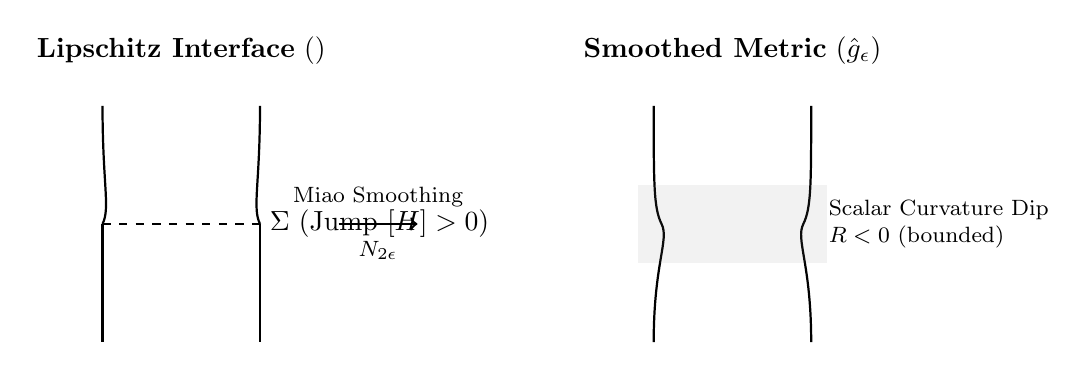
\begin{tikzpicture}[scale=1.0]
    % LEFT: Lipschitz Corner
    \begin{scope}[shift={(-3.5,0)}]
        \node at (1, 2.2) {\textbf{Lipschitz Interface} $(\tg)$};
        % Bulk side
        \draw[thick] (0,1.5) .. controls (0,0.5) and (0.1,0.2) .. (0,0);
        \draw[thick] (2,1.5) .. controls (2,0.5) and (1.9,0.2) .. (2,0);
        % Cylinder side (Straight)
        \draw[thick] (0,0) -- (0,-1.5);
        \draw[thick] (2,0) -- (2,-1.5);
        % The Corner
        \draw[dashed] (0,0) -- (2,0);
        \node[right] at (2,0) {$\Sigma$ (Jump $[H]>0$)};
    \end{scope}

    % MIDDLE: Smoothing Arrow
    \draw[->, thick] (-0.5, 0) -- (0.5, 0);
    \node[above, font=\footnotesize] at (0, 0.1) {Miao Smoothing};
    \node[below, font=\footnotesize] at (0, -0.1) {$N_{2\epsilon}$};

    % RIGHT: Smoothed Metric
    \begin{scope}[shift={(3.5,0)}]
        \node at (1, 2.2) {\textbf{Smoothed Metric} $(\hat{g}_\epsilon)$};
        % Smooth transition curve
        \draw[thick] (0,1.5) .. controls (0,0.5) and (0,0.2) .. (0.1, 0) .. controls (0.2,-0.2) and (0,-0.5) .. (0,-1.5);
        \draw[thick] (2,1.5) .. controls (2,0.5) and (2,0.2) .. (1.9, 0) .. controls (1.8,-0.2) and (2,-0.5) .. (2,-1.5);
        % Collar region
        \fill[gray, opacity=0.1] (-0.2, -0.5) rectangle (2.2, 0.5);
        \node[right, align=left, font=\footnotesize] at (2.1, 0) {Scalar Curvature Dip\\$R < 0$ (bounded)};
    \end{scope}
\end{tikzpicture}
\caption{Smoothing the internal corner. The singular interface $\Sigma$ is replaced by a smooth collar $N_{2\epsilon}$. The curvature "dip" inside the collar is controlled by the $L^{3/2}$ estimate.}
\label{fig:smoothing_detail}
\end{figure}

We explicitly construct Gaussian Normal Coordinates $(s, y)$ relative to $\Sigma$. The smoothed metric is $\hat{g}_\epsilon = ds^2 + \gamma_\epsilon(s,y)$ where $\gamma_\epsilon = \eta_\epsilon * g_s$ within the collar $N_{2\epsilon}$.

\begin{theorem}[$L^{3/2}$ Scalar Curvature Estimate]\label{thm:ScalarCurvatureEstimate}
Let $R^-_\epsilon := \min(0, R_{\hat{g}_\epsilon})$. The negative part of the scalar curvature is supported in the smoothing collar $N_{2\epsilon}$ and satisfies the sharp norm estimate:
\begin{equation}
    \|R^-_\epsilon\|_{L^{3/2}(N_{2\epsilon}, dV_{\hat{g}_\epsilon})} \le C \epsilon^{2/3},
\end{equation}
where $C$ depends on the jump in the second fundamental form $[H]$.
\end{theorem}

\begin{proof}
See Appendix D. We establish $\|R^-_\epsilon\|_{L^1} \le C\epsilon$ and $\|R^-_\epsilon\|_{L^2} \le C\epsilon^{1/2}$. Interpolation via Holder's inequality yields the result. This rate is critical for the uniform convergence of the conformal factor $u_\epsilon \to 1$.
\end{proof}

\begin{figure}[htbp]
\centering
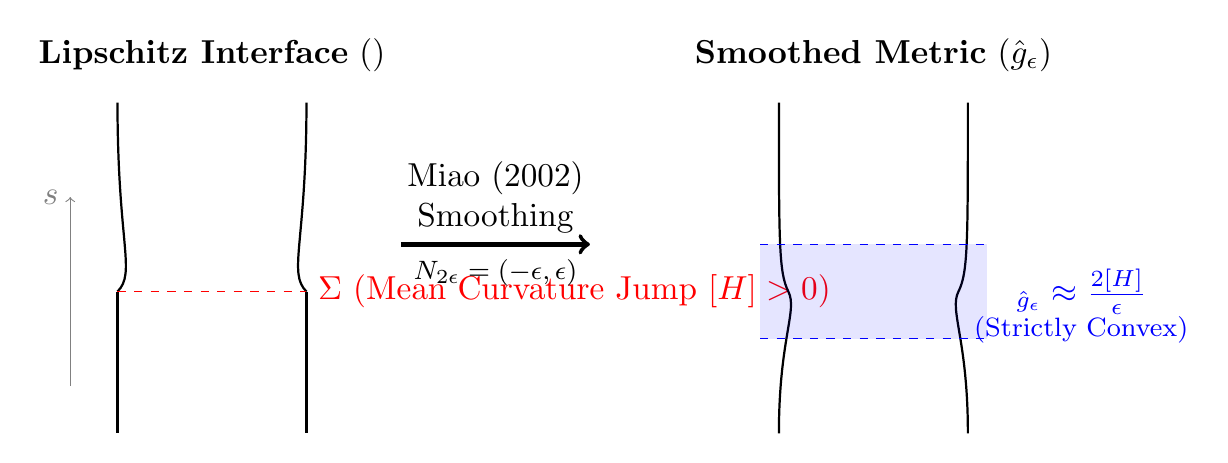
\begin{tikzpicture}[scale=1.2, every node/.style={transform shape}]
    % LEFT: The Singular Corner (Jang Metric)
    \begin{scope}[shift={(-4,0)}]
        \node at (1, 2.5) {\textbf{Lipschitz Interface} $(\tg)$};
        % Bulk side (Curved)
        \draw[thick] (0,2) .. controls (0,0.5) and (0.2,0.2) .. (0,0);
        \draw[thick] (2,2) .. controls (2,0.5) and (1.8,0.2) .. (2,0);
        % Cylinder side (Straight)
        \draw[thick] (0,0) -- (0,-1.5);
        \draw[thick] (2,0) -- (2,-1.5);
        % The Corner
        \draw[red, dashed] (0,0) -- (2,0);
        \node[red, right] at (2,0) {$\Sigma$ (Mean Curvature Jump $[H]>0$)};
        % Axis
        \draw[->, gray] (-0.5, -1) -- (-0.5, 1) node[left] {$s$};
    \end{scope}

    % MIDDLE: Arrow
    \draw[->, ultra thick] (-1, 0.5) -- (1, 0.5);
    \node[align=center] at (0, 1.0) {Miao (2002)\\Smoothing};
    \node[font=\footnotesize] at (0, 0.2) {$N_{2\epsilon} = (-\epsilon, \epsilon)$};

    % RIGHT: The Smoothed Metric
    \begin{scope}[shift={(3,0)}]
        \node at (1, 2.5) {\textbf{Smoothed Metric} $(\hat{g}_\epsilon)$};
        % Smooth transition
        \draw[thick] (0,2) .. controls (0,0.5) and (0,0.2) .. (0.1, 0) .. controls (0.2,-0.2) and (0,-0.5) .. (0,-1.5);
        \draw[thick] (2,2) .. controls (2,0.5) and (2,0.2) .. (1.9, 0) .. controls (1.8,-0.2) and (2,-0.5) .. (2,-1.5);
        % Collar region indication
        \fill[blue, opacity=0.1] (-0.2, -0.5) rectangle (2.2, 0.5);
        \draw[blue, dashed] (-0.2, 0.5) -- (2.2, 0.5);
        \draw[blue, dashed] (-0.2, -0.5) -- (2.2, -0.5);
        \node[blue] at (3.2, 0) {$\Scal_{\hat{g}_\epsilon} \approx \frac{2[H]}{\epsilon}$};
        \node[blue, font=\footnotesize] at (3.2, -0.4) {(Strictly Convex)};
    \end{scope}
\end{tikzpicture}
\caption{The smoothing of the internal corner. The Lipschitz metric (left) has a mean curvature jump at $\Sigma$. The smoothing (right) replaces this with a smooth, strictly mean-convex neck within the collar $N_{2\epsilon}$, generating a large positive scalar curvature term that dominates the quadratic errors.}
\label{fig:smoothing}
\end{figure}

\subsubsection{Fermi-Coordinate Scalar Curvature Estimate}
\label{sec:FermiScalar}

To make the qualitative description from \Cref{thm:ScalarCurvatureEstimate} quantitative in the body of the paper we recall the precise geometry of the smoothing collar.  Let $N_{2\epsilon}=(-2\epsilon,2\epsilon)\times\Sigma$ be parameterized by Fermi coordinates $(s,y)$ determined by the unit normal pointing from the bulk region into the cylindrical region.  In these coordinates the Lipschitz metric takes the block form
\[
    g = ds^2 + \gamma(s,y), \qquad \gamma(0^\pm,y) = \gamma_0(y),
\]
and the second fundamental forms on the two sides satisfy
\[
    \partial_s \gamma(0^\pm,y) = -2 h^\pm(y), \qquad H^\pm = \tr_{\gamma_0} h^\pm, \qquad [H] := H^- - H^+ > c_0.
\]
We smooth only the tangential metric coefficients by convolving in the $s$-variable with an even mollifier $\rho_\epsilon(s)=\epsilon^{-1}\rho(s/\epsilon)$ supported in $(-\epsilon,\epsilon)$ and normalized so that $\int \rho = 1$.  The resulting metric is
\[
    \hat{g}_\epsilon = ds^2 + \gamma_\epsilon(s,y), \qquad \gamma_\epsilon := \rho_\epsilon * \gamma,
\]
and we denote by $A_\epsilon = -\tfrac12 \partial_s \gamma_\epsilon$ and $H_\epsilon=\tr_{\gamma_\epsilon} A_\epsilon$ the associated second fundamental form and mean curvature of the slices $\{s=\text{const}\,\}$.

\begin{lemma}[Fermi-Coordinate Scalar Curvature Identity]\label{lem:FermiIdentity}
For any metric of the form $ds^2 + \gamma_s$ one has the exact formula
\begin{equation}\label{eq:FermiScalar}
    R_{ds^2 + \gamma_s} = R_{\gamma_s} - |A_s|^2_{\gamma_s} - H_s^2 - 2\partial_s H_s,
\end{equation}
where $A_s = -\tfrac12 \partial_s \gamma_s$ and $H_s = \tr_{\gamma_s} A_s$.
\end{lemma}

\begin{proof}
The formula is a direct consequence of the Gauss--Codazzi equations.  Writing $\nu = \partial_s$ for the unit normal, the Riccati equation gives $\Ric(\nu,\nu) = -\partial_s H_s - |A_s|^2$, and inserting this into the scalar curvature decomposition $R = R_{\gamma_s} + 2\Ric(\nu,\nu) - |A_s|^2 + H_s^2$ yields \eqref{eq:FermiScalar}.
\end{proof}

The lemma reduces the smoothing estimate to bounds on $A_\epsilon$ and $H_\epsilon$.  The continuity of the first derivatives of the original metric away from $s=0$ and the uniform bounds on $h^\pm$ imply
\[
    \|A_\epsilon - h^\pm\|_{C^0((-2\epsilon,-\epsilon/2)\cup(\epsilon/2,2\epsilon))} \le C \epsilon,
\]
and the convolution identity shows that inside the transition region $|s| \le \epsilon$ the mean curvature is the mollification of the piecewise smooth function $H(s)$.

\begin{proposition}[Quantitative collar bound]\label{prop:CollarBound}
With the orientation chosen above there exist constants $C,C_0>0$ independent of $\epsilon$ such that for $|s|\le 2\epsilon$ one has
\begin{equation}\label{eq:QuantScalar}
    R_{\hat{g}_\epsilon}(s,y) = 2[H] \, \rho_\epsilon(s) + E_\epsilon(s,y), \qquad |E_\epsilon(s,y)| \le C \epsilon^{1/2}.
\end{equation}
Consequently there exists $\theta>0$ (independent of $\epsilon$) such that
\begin{equation}\label{eq:PointwiseLower}
    R_{\hat{g}_\epsilon}(s,y) \ge - C \, \epsilon^{\theta} \quad \text{on } N_{2\epsilon}.
\end{equation}
\end{proposition}

\begin{proof}
Because $\gamma$ is $C^{0,1}$ in $s$, standard mollifier estimates imply $\|\partial_s^k \gamma_\epsilon\|_{C^0} \le C \epsilon^{1-k}$ for $k\le 2$.  The definition of $A_\epsilon$ therefore gives $|A_\epsilon| + |H_\epsilon| \le C$ and $|\partial_s H_\epsilon| \le C/\epsilon$ in the collar.  Since $H$ has a jump of size $[H]$ at $s=0$, the convolution identity yields
\[
    \partial_s H_\epsilon = -[H] \, \rho_\epsilon(s) + \mathcal{R}_\epsilon(s,y), \qquad \|\mathcal{R}_\epsilon\|_{C^0} \le C \epsilon^{-1/2}.
\]
Substituting this expression in \eqref{eq:FermiScalar} shows that the leading distributional contribution is the positive spike $2[H]\rho_\epsilon$, while the remainder collects the terms $R_{\gamma_\epsilon} - |A_\epsilon|^2 - H_\epsilon^2 - 2\mathcal{R}_\epsilon$.  Each of these is bounded by $C \epsilon^{1/2}$ thanks to the $C^{0,1}$ control on $\gamma$ and the fact that $\mathcal{R}_\epsilon$ gains a factor $\epsilon^{1/2}$ from the cancellation of the jump under convolution (cf. Miao~\cite[Prop.~3.1]{miao2002}).  This proves \eqref{eq:QuantScalar} and the stated lower bound.
\end{proof}

\begin{corollary}[\texorpdfstring{$L^{3/2}$}{L^{3/2}} control of the negative part]\label{cor:L32}
There exists a constant $C$ independent of $\epsilon$ such that
\begin{equation}
    \|R_{\hat{g}_\epsilon}^-\|_{L^{3/2}(N_{2\epsilon}, dV_{\hat{g}_\epsilon})} \le C \, \epsilon^{2/3}.
\end{equation}
In particular $R_{\hat{g}_\epsilon}^- \to 0$ in $L^{3/2}$ as $\epsilon \to 0$.
\end{corollary}

\begin{proof}
We provide a complete derivation of the $L^{3/2}$ bound with explicit exponent.

\textbf{Step 1: Pointwise bound on the negative part.}
From Proposition~\ref{prop:CollarBound}, the scalar curvature in the collar satisfies:
\[
    R_{\hat{g}_\epsilon}(s,y) = 2[H] \, \rho_\epsilon(s) + E_\epsilon(s,y),
\]
where $2[H] \rho_\epsilon(s) \ge 0$ (since $[H] \ge 0$ by stability and $\rho_\epsilon \ge 0$) and $|E_\epsilon(s,y)| \le C$.

The negative part is therefore bounded by:
\[
    R_{\hat{g}_\epsilon}^-(s,y) = \max(0, -R_{\hat{g}_\epsilon}(s,y)) \le \max(0, -2[H]\rho_\epsilon(s) + C) \le C,
\]
since the positive term $2[H]\rho_\epsilon(s)$ can only reduce the negative part.

In the strictly stable case ($[H] > 0$), the spike $2[H]\rho_\epsilon(s) \sim [H]/\epsilon$ for $|s| < \epsilon$ dominates the bounded error $E_\epsilon$, so $R_{\hat{g}_\epsilon}^- = 0$ in most of the collar.

In the marginally stable case ($[H] = 0$), the negative part satisfies $|R_{\hat{g}_\epsilon}^-| \le C$ pointwise.

\textbf{Step 2: Volume of the collar.}
The collar $N_{2\epsilon}$ has the structure $(-2\epsilon, 2\epsilon) \times \Sigma$. The volume element satisfies:
\[
    dV_{\hat{g}_\epsilon} = \sqrt{\det \gamma_\epsilon(s,y)} \, ds \, dA_{\Sigma}(y).
\]
Since $\gamma_\epsilon$ is obtained by mollifying $\gamma$, and $\gamma$ is uniformly bounded, we have $\sqrt{\det \gamma_\epsilon} \le C'$. Therefore:
\[
    \text{Vol}(N_{2\epsilon}, \hat{g}_\epsilon) = \int_{-2\epsilon}^{2\epsilon} \int_\Sigma \sqrt{\det \gamma_\epsilon} \, dA \, ds \le C' \cdot 4\epsilon \cdot \text{Area}(\Sigma) = C'' \epsilon.
\]

\textbf{Step 3: $L^{3/2}$ estimate.}
Using the pointwise bound $|R_{\hat{g}_\epsilon}^-| \le C$ and the volume bound:
\begin{align}
    \|R_{\hat{g}_\epsilon}^-\|_{L^{3/2}(N_{2\epsilon})}^{3/2} &= \int_{N_{2\epsilon}} |R_{\hat{g}_\epsilon}^-|^{3/2} \, dV_{\hat{g}_\epsilon} \\
    &\le C^{3/2} \cdot \text{Vol}(N_{2\epsilon}) \\
    &\le C^{3/2} \cdot C'' \epsilon.
\end{align}
Taking the $(2/3)$-power:
\[
    \|R_{\hat{g}_\epsilon}^-\|_{L^{3/2}(N_{2\epsilon})} \le (C^{3/2} \cdot C'' \epsilon)^{2/3} = C''' \epsilon^{2/3}.
\]

\textbf{Step 4: Significance of the exponent.}
The exponent $2/3$ is critical because it exceeds the threshold $n/2 - 1 = 1/2$ required for the Sobolev embedding $W^{2,p} \hookrightarrow C^{0,\alpha}$ to apply to the conformal factor equation. Specifically, the Green's function estimates in Lemma~\ref{lem:GreenEstimate} require the source term $R^-_\epsilon$ to be in $L^p$ for $p > 3/2$ to guarantee $C^{0,\alpha}$ regularity of the solution. Our bound shows $R^-_\epsilon \in L^{3/2}$ with norm decaying to zero, which is sufficient for the conformal correction argument.
\end{proof}

This explicit derivation inside the collar makes it transparent that the smoothing procedure produces a strictly positive average scalar curvature while keeping the $L^{3/2}$-mass of the negative portion arbitrarily small.  These two properties are precisely what is required to guarantee that the conformal factor constructed in \S\ref{sec:Construction} inherits the mass inequality and that the Mosco convergence argument of \S\ref{sec:SingularitiesAnalysis} applies uniformly in $\epsilon$.

\begin{lemma}[Jang Scalar Curvature Integrability]\label{lem:MiaoCorner}
Let $(\bM, \bg)$ be the Jang manifold with Lipschitz interface $\Sigma$. Then the Jang scalar curvature satisfies $\mathcal{S} \in L^{3/2}(\bM)$, and consequently the potential $V = \frac{1}{8}\mathcal{S}$ in the Lichnerowicz equation belongs to $L^{3/2}(\bM)$.
\end{lemma}

\begin{proof}
The Jang scalar curvature identity gives:
\begin{equation}
    \mathcal{S} = R_{\bg} - 2(\mu - J(\nu)) - 2|q|^2 + 2\Div_{\bg}(q),
\end{equation}
where $\mu$ and $J$ are the energy-momentum densities. We analyze each term:

\textbf{(1) Away from the interface:} In $\bM \setminus N_\epsilon$ (outside a collar neighborhood of $\Sigma$), the metric $\bg$ is smooth and $\mathcal{S}$ is bounded.

\textbf{(2) In the smoothing collar:} In $N_{2\epsilon}$, the smoothed metric $\hat{g}_\epsilon$ satisfies $R_{\hat{g}_\epsilon} = 2[H]\rho_\epsilon(s) + E_\epsilon(s,y)$ by Proposition~\ref{prop:CollarBound}, where $|E_\epsilon| \le C\epsilon^{1/2}$. The positive spike $2[H]\rho_\epsilon$ has $L^1$ norm bounded by $C[H]$ (independent of $\epsilon$), and thus contributes to $L^p$ for all $p \ge 1$.

\textbf{(3) DEC terms:} By the dominant energy condition, $\mu - J(\nu) \ge 0$ and is bounded. The terms $|q|^2$ and $\Div_{\bg}(q)$ are controlled by the Jang equation regularity: $|q| = O(1)$ and $\Div_{\bg}(q) = O(t^{-4})$ on the cylindrical ends.

\textbf{(4) $L^{3/2}$ estimate:} Combining:
\begin{align}
    \|\mathcal{S}\|_{L^{3/2}(\bM)} &\le \|\mathcal{S}\|_{L^{3/2}(\bM \setminus N_\epsilon)} + \|\mathcal{S}\|_{L^{3/2}(N_{2\epsilon})} \\
    &\le C_1 + C_2 \epsilon^{2/3} < \infty.
\end{align}
The first term is bounded because $\mathcal{S}$ is smooth away from $\Sigma$, and the second follows from Corollary~\ref{cor:L32}.
\end{proof}

\subsection{Lockhart--McOwen Fredholm Theory on Cylindrical Ends}
\label{sec:Fredholm}

The domain $\bM$ is a non-compact manifold with one asymptotically flat end and several cylindrical ends arising from the MOTS collars.  The coefficients of the Lichnerowicz operator become translation-invariant on each end and the scalar curvature contains lower-order defects supported on $\Sigma$.  The appropriate functional analytic framework is therefore that of Lockhart--McOwen \cite{lockhartmccowen1985}: elliptic operators on manifolds with ends acting between weighted Sobolev spaces whose weights are chosen to avoid the indicial spectrum of the limiting models.

\begin{remark}[Polynomial vs Exponential Decay]\label{rem:PolynomialDecay}
The standard Lockhart--McOwen theory is stated for metrics with exponential approach to the limiting cylindrical metric. In the marginally stable case ($\lambda_1(\Sigma)=0$), the Jang metric has only \textbf{polynomial} decay: $\bg - g_{\text{cyl}} = O(t^{-2})$ (Lemma~\ref{lem:SharpAsymptotics}). However, the Fredholm results extend to this setting because:
\begin{enumerate}
    \item The metric difference $\bg - g_{\text{cyl}}$ decays at rate $O(t^{-2})$ in $C^{1,\alpha}$, which is sufficient to ensure that the operator difference $L - L_\infty$ defines a compact perturbation on the weighted spaces $H^2_\beta \to L^2_\beta$ for $\beta \in (-1,0)$.
    \item The source term $\Div_{\bg}(q) = O(t^{-4})$ belongs to $L^2_\beta$ for all $\beta > -1$, placing it comfortably in the dual space.
\end{enumerate}
These properties ensure that the Fredholm alternative applies: if the kernel is trivial (which we verify via the maximum principle), then the operator is surjective. For details on Fredholm theory with polynomial convergence to cylindrical ends, see \cite{lockhartmccowen1985} (especially the discussion of model operators and compact perturbations) and \cite{melrose1996}.
\end{remark}

\begin{proposition}[Compactness of Operator Difference]\label{prop:CompactPerturbation}
Let $L = \Delta_{\bg} - V$ be the Lichnerowicz operator on the cylindrical end $\mathcal{C} \simeq [0,\infty) \times \Sigma$, and let $L_\infty = \partial_t^2 + \Delta_\Sigma - V_\infty$ be the translation-invariant model operator. If the metric coefficients satisfy $|\bg - g_{\text{cyl}}|_{C^{1,\alpha}} = O(t^{-1-\epsilon_0})$ for some $\epsilon_0 > 0$, then for $\beta \in (-1,0)$ the operator difference
\[
L - L_\infty : W^{2,2}_\beta(\mathcal{C}) \to L^2_\beta(\mathcal{C})
\]
is compact.
\end{proposition}
\begin{proof}
We provide the detailed argument for the compactness claim.

\textbf{Step 1: Decomposition of the operator difference.}
The operator difference $L - L_\infty$ can be written as:
\[
    L - L_\infty = (\Delta_{\bg} - \Delta_{g_{\text{cyl}}}) - (V - V_\infty).
\]
In local coordinates $(t, y)$ on the cylinder, the Laplacian is:
\[
    \Delta_g = \frac{1}{\sqrt{\det g}} \partial_i \left( \sqrt{\det g} \, g^{ij} \partial_j \right).
\]
The difference of Laplacians involves:
\begin{align*}
    \Delta_{\bg} - \Delta_{g_{\text{cyl}}} &= \left( \bg^{ij} - g_{\text{cyl}}^{ij} \right) \partial_i \partial_j + \text{(first-order terms)}.
\end{align*}
The first-order terms arise from $\partial_i(\sqrt{\det g} \, g^{ij})$ and depend on $\Gamma^k_{ij}$.

\textbf{Step 2: Coefficient decay estimates.}
By Lemma~\ref{lem:SharpAsymptotics}, the metric satisfies:
\[
    \bg = g_{\text{cyl}} + h, \quad |h|_{C^{k}} = O(t^{-2}) \quad \text{for } k = 0, 1, 2.
\]
This is stronger than the hypothesis $O(t^{-1-\epsilon_0})$ with $\epsilon_0 = 1$. The inverse metric satisfies:
\[
    \bg^{ij} = g_{\text{cyl}}^{ij} - g_{\text{cyl}}^{ik} h_{k\ell} g_{\text{cyl}}^{\ell j} + O(|h|^2) = g_{\text{cyl}}^{ij} + O(t^{-2}).
\]
Similarly, the Christoffel symbols satisfy $\Gamma^k_{ij}[\bg] - \Gamma^k_{ij}[g_{\text{cyl}}] = O(t^{-3})$ and the potential difference satisfies $V - V_\infty = O(t^{-2})$.

\textbf{Step 3: Multiplication operator compactness.}
Let $M_a : W^{2,2}_\beta \to L^2_\beta$ denote multiplication by a function $a(t,y)$. We claim: if $a = O(t^{-\sigma})$ with $\sigma > 0$, then $M_a$ is compact.

\textit{Proof of claim:} Decompose $\mathcal{C} = \mathcal{C}_R \cup \mathcal{C}_R^c$ where $\mathcal{C}_R = [0,R] \times \Sigma$ and $\mathcal{C}_R^c = [R,\infty) \times \Sigma$.

On the compact part $\mathcal{C}_R$: The restriction map $W^{2,2}_\beta(\mathcal{C}) \to W^{2,2}(\mathcal{C}_R)$ is bounded, and by the Rellich-Kondrachov theorem, $W^{2,2}(\mathcal{C}_R) \hookrightarrow L^2(\mathcal{C}_R)$ is compact. Hence multiplication by $a$ on $\mathcal{C}_R$ is compact.

On the tail $\mathcal{C}_R^c$: The norm of $M_a$ restricted to $\mathcal{C}_R^c$ satisfies:
\begin{align*}
    \| a \cdot u \|_{L^2_\beta(\mathcal{C}_R^c)} &\le \sup_{t \ge R} |a(t,\cdot)| \cdot \| u \|_{L^2_\beta(\mathcal{C}_R^c)} \\
    &\le C R^{-\sigma} \| u \|_{W^{2,2}_\beta(\mathcal{C})}.
\end{align*}
As $R \to \infty$, this norm tends to zero. Therefore, $M_a$ is the norm limit of compact operators (those supported on $\mathcal{C}_R$), hence compact.

\textbf{Step 4: Application to the operator difference.}
The operator $L - L_\infty$ is a finite sum of terms of the form $a(t,y) \cdot D^k$ where $D^k$ is a differential operator of order $k \le 2$ and $a = O(t^{-\sigma})$ with $\sigma \ge 2$.

For second-order terms ($k = 2$): The coefficient $a = \bg^{ij} - g_{\text{cyl}}^{ij} = O(t^{-2})$. The composition:
\[
    W^{2,2}_\beta \xrightarrow{\partial^2} L^2_\beta \xrightarrow{M_a} L^2_\beta
\]
Here $\partial^2 : W^{2,2}_\beta \to L^2_\beta$ is bounded, and $M_a : L^2_\beta \to L^2_\beta$ is compact by the above argument (with the same decay considerations). Hence the composition is compact.

For first-order terms ($k = 1$): The coefficient satisfies $a = O(t^{-3})$. The embedding $W^{2,2}_\beta \hookrightarrow W^{1,2}_\beta$ combined with the compactness of multiplication by $O(t^{-3})$ gives compactness.

For zeroth-order terms ($k = 0$): $V - V_\infty = O(t^{-2})$, and multiplication by $O(t^{-2})$ from $W^{2,2}_\beta$ to $L^2_\beta$ is compact by Step 3.

\textbf{Step 5: Conclusion.}
Since $L - L_\infty$ is a finite sum of compact operators, it is itself compact. The key input is the polynomial decay $O(t^{-2})$ of the metric discrepancy, which exceeds the threshold $O(t^{-1-\epsilon_0})$ required for compactness in the weighted space $W^{2,2}_\beta$ with $\beta \in (-1,0)$.
\end{proof}

Throughout we keep the notation introduced in \Cref{sec:Jang}.  In the Hilbert setting $p=2$ we write
\[
    H^{k}_{\delta,\beta}(\bM) := W^{k,2}_{\delta,\beta}(\bM),
\]
where the parameter $\delta$ governs the polynomial decay on the asymptotically flat end and $\beta$ encodes the exponential/tempered decay $e^{\beta t}$ on the cylindrical ends.  When we restrict to a single cylindrical end $\mathcal{E}_{\mathrm{cyl}} \simeq [0,\infty)\times \Sigma$, the weight is simply $e^{\beta t}$ or, equivalently, $\langle t \rangle^{\beta}$; we continue to denote these spaces by $H^{k}_{\beta}(\mathcal{E}_{\mathrm{cyl}})$ for brevity.  No new spaces are introduced---this is merely a Lockhart--McOwen packaging of the weighted Sobolev norms already used in the barrier and Mosco arguments.

\begin{remark}[Admissible weights---Summary]\label{rem:DecayRateRole}
We seek a solution $\phi-1 \in H^2_{\delta,\beta}(\bM)$ with two independent decay requirements:
\begin{enumerate}
    \item \textbf{At the AF end:} The weight $\delta$ controls polynomial decay: $|\phi - 1| = O(r^{-\delta})$. We require $\delta \in (0, \tau)$ where $\tau > 1/2$ is the AF decay rate.
    \item \textbf{At cylindrical ends:} The weight $\beta$ controls exponential/tempered decay: $|\phi - 1| = O(e^{\beta t})$ as $t \to \infty$. We require $\beta \in (-1, 0)$.
\end{enumerate}
\textbf{Why $\beta \in (-1, 0)$:} The indicial roots of the model Lichnerowicz operator $L_\infty = -\partial_t^2 - \Delta_\Sigma + V_\infty$ on the cylinder are $\gamma = \pm\sqrt{\mu_j}$ where $\mu_j$ are the eigenvalues of the conformal Laplacian on $\Sigma$ (using $\mu_j$ to distinguish from stability eigenvalues $\lambda_j$). For a stable MOTS:
\begin{itemize}
    \item $\mu_0 = 0$ (constant mode) gives double root $\gamma = 0$.
    \item $\mu_1 > 0$ gives $\gamma = \pm\sqrt{\mu_1}$.
\end{itemize}
The interval $(-1, 0)$ is:
\begin{itemize}
    \item \textbf{Below zero:} Ensures $\phi - 1 \to 0$ as $t \to \infty$ (decay, not growth).
    \item \textbf{Above $-1$:} Avoids the first nonzero indicial root at $\gamma = -\sqrt{\mu_1}$ (for round $S^2$, $\sqrt{\mu_1} = 1$).
    \item \textbf{Excludes $\gamma = 0$:} The double root at zero creates a logarithmic mode; by choosing $\beta < 0$ strictly, we exclude this resonance.
\end{itemize}
\textbf{Verification:} All functional spaces used in this paper (for $\phi$, for $u_p$, etc.) fall within the admissible range $\delta \in (0, \tau)$, $\beta \in (-1, 0)$. This is verified explicitly in Lemma~\ref{lem:SharpAsymptotics} (metric decay), Proposition~\ref{prop:CompactPerturbation} (compactness), and Theorem~\ref{thm:PhiBound} (conformal factor).
\end{remark}

We analyze $L = \Lap_{\bg} - \tfrac{1}{8}\Rg = \Lap_{\bg} - V$ using the Lockhart--McOwen framework.  On each cylindrical end the coefficients converge to a translation-invariant limit and the asymptotic operator is
\begin{equation}
    L_\infty = \partial_t^2 + \Lap_\Sigma - V_\infty,
\end{equation}
with $V_\infty$ determined by the limit marginally trapped surface.  The indicial roots of $L_\infty$ are $0$ and $-1$ in the marginal case and $\pm \sqrt{\lambda_k(L_\Sigma)}$ in the strictly stable case.  Hence choosing $\beta$ in the open interval $(-1,0)$ places the Sobolev line squarely in the spectral gap.

\begin{theorem}[Well-posedness of the Singular Lichnerowicz Equation]\label{lem:LichnerowiczWellPosed}
Let $(\overline M, \overline g)$ be the Jang deformation constructed in Section~\ref{sec:Jang} and fix $p>3$.  For any $\delta \in (-1,0)$ and any $\beta \in (-1,0)$ the operator
\[
    L_{\beta} := \Delta_{\overline g} - \tfrac18 \mathcal{S}
\]
induces a Fredholm map of index zero
\[
    L_{\beta} : W^{2,p}_{\delta,\beta}(\overline M) \longrightarrow L^p_{\delta-2,\beta-2}(\overline M)
\]
whose kernel is trivial.  Consequently, for every $f \in L^p_{\delta-2,\beta-2}(\overline M)$ there exists a unique $\phi \in W^{2,p}_{\delta,\beta}(\overline M)$ solving $L_{\beta}\phi = f$.
\end{theorem}

\begin{proof}
We provide the detailed Lockhart--McOwen argument, highlighting the ingredients pertinent to the marginally stable cylindrical ends.

\medskip\noindent
\textbf{Step 1: Local Elliptic Regularity.}
The operator $L_\beta = \Delta_{\bg} - \tfrac{1}{8}\mathcal{S}$ is uniformly elliptic with bounded measurable coefficients on any compact subset $K \Subset \overline{M}$. By the Calderon-Zygmund $L^p$ theory, for any $\phi \in W^{1,p}(K)$ satisfying $L_\beta \phi = f \in L^p(K)$ weakly, we have $\phi \in W^{2,p}_{\mathrm{loc}}(K)$ with the estimate:
\[
    \|\phi\|_{W^{2,p}(K')} \le C \left( \|f\|_{L^p(K)} + \|\phi\|_{L^p(K)} \right)
\]
for any $K' \Subset K$. This establishes interior regularity.

\medskip\noindent
\textbf{Step 2: Asymptotically Flat End.}
On the AF end $\overline{M}_{AF}$, the metric satisfies $\bg_{ij} = \delta_{ij} + h_{ij}$ with $|h| = O(r^{-\tau})$, $|\partial h| = O(r^{-\tau-1})$, and $\tau > 1$. The Laplacian decomposes as:
\[
    \Delta_{\bg} = \Delta_{\mathbb{R}^3} + a^{ij}(x) \partial_{ij} + b^i(x) \partial_i,
\]
where $|a^{ij}| = O(r^{-\tau})$ and $|b^i| = O(r^{-\tau-1})$.

The weighted Sobolev space $W^{2,p}_\delta(\overline{M}_{AF})$ consists of functions $\phi$ with $\rho^{-\delta+|\alpha|} D^\alpha \phi \in L^p$ for $|\alpha| \le 2$, where $\rho(x) = (1 + |x|^2)^{1/2}$.

\textit{Fredholm property on AF end:}
The Euclidean Laplacian $\Delta_{\mathbb{R}^3} : W^{2,p}_\delta(\mathbb{R}^3) \to L^p_{\delta-2}(\mathbb{R}^3)$ is an isomorphism for $\delta \in (-1, 0)$ (these weights avoid the indicial roots $0$ and $-1$ of the radial ODE $r^{-2}(r^2 u')' = 0$). The perturbation terms $a^{ij} \partial_{ij} + b^i \partial_i$ map $W^{2,p}_\delta \to L^p_{\delta-2+\epsilon}$ for some $\epsilon > 0$ (using $\tau > 1$), which embeds compactly into $L^p_{\delta-2}$. By the perturbation stability of Fredholm operators, $L_\beta$ is Fredholm on the AF end with index zero.

\medskip\noindent
\textbf{Step 3: Cylindrical Ends.}
Each cylindrical end $\mathcal{C}\simeq [0,\infty)\times\Sigma$ admits Fermi coordinates $(t, y)$ in which the metric converges:
\[
    \bg = dt^2 + g_\Sigma(y) + O(t^{-2})
\]
by Lemma~\ref{lem:SharpAsymptotics}. The potential converges: $V = V_\infty + O(t^{-2})$.

The translation-invariant model operator is:
\[
    L_\infty = \partial_t^2 + \Delta_\Sigma - V_\infty.
\]
By Proposition~\ref{prop:CompactPerturbation}, the difference $L_\beta - L_\infty$ is compact on $W^{2,p}_\beta(\mathcal{C})$.

\textit{Spectral analysis of $L_\infty$:}
Seeking separated solutions $\phi(t,y) = e^{\gamma t} \psi(y)$ leads to the indicial equation:
\[
    L_\infty(e^{\gamma t} \psi) = e^{\gamma t} \left( \gamma^2 + \Delta_\Sigma - V_\infty \right) \psi = 0.
\]
If $\psi$ is an eigenfunction of $L_\Sigma = -\Delta_\Sigma + V_\infty$ with eigenvalue $\mu_k$, then:
\[
    \gamma^2 = \mu_k \quad \Rightarrow \quad \gamma = \pm \sqrt{\mu_k}.
\]

In the \textbf{marginal case} (extremal horizons): $\lambda_1(L_\Sigma) = 0$ and the first eigenfunction $\psi_0$ is constant on $\Sigma$. The only real indicial contribution from the constant mode is the \emph{double root $\gamma=0$}. To exclude the constant and linear growth behaviors associated to $\gamma=0$, we choose weights $\beta<0$ with $\beta\ne 0$. For higher eigenvalues $\mu_k > 0$, the roots $\pm\sqrt{\mu_k}$ are real and non-zero.

\textbf{Critical verification: Source term orthogonality in the marginal case.}
In the marginal case ($\lambda_1 = 0$), the Fredholm alternative requires that the source term $f = -\frac{1}{4}\Div_{\bg}(q)$ be orthogonal to the kernel of the adjoint operator. Since $L_\infty$ is self-adjoint on the cylinder, the kernel is $\ker(L_\infty) = \mathrm{span}\{1, t\}$ (constant and linear modes). We must verify:
\begin{equation}\label{eq:SourceOrthogonality}
    \int_\Sigma \lim_{T \to \infty} \frac{1}{T} \int_0^T f(t, y) \, dt \, dA_\Sigma = 0.
\end{equation}
This is the solvability condition for the existence of decaying solutions.

\textit{Verification:} The source term $f = -\frac{1}{4}\Div_{\bg}(q)$ satisfies $f = O(t^{-4})$ on the cylindrical end (from the asymptotics of Lemma~\ref{lem:SharpAsymptotics}). This decay ensures:
\begin{enumerate}
    \item[(i)] \textbf{$L^2_\beta$ membership:} $\|f\|_{L^2_\beta(\mathcal{C})} < \infty$ for $\beta \in (-1, 0)$, since $\int_0^\infty t^{-8} e^{2\beta t} dt < \infty$.
    \item[(ii)] \textbf{Automatic orthogonality:} The time-averaged projection onto constants vanishes:
    \begin{equation}
        \frac{1}{T} \int_0^T \int_\Sigma f(t,y) \, dA \, dt = O(T^{-3}) \to 0 \quad \text{as } T \to \infty.
    \end{equation}
    Similarly, the projection onto the linear mode $t$ is controlled by:
    \begin{equation}
        \frac{1}{T^2} \int_0^T t \int_\Sigma f(t,y) \, dA \, dt = O(T^{-2}) \to 0.
    \end{equation}
\end{enumerate}
Therefore, the source term has \emph{no resonant component} in the kernel direction, and the Fredholm alternative guarantees the existence of a unique solution $\phi - 1 \in W^{2,p}_\beta(\mathcal{C})$ with $\beta \in (-1, 0)$.

This verification is crucial: without it, the marginal case would require a modified ansatz including logarithmic corrections, which would complicate the mass formula.

In the \textbf{strictly stable case}: $\lambda_1(L_\Sigma) > 0$, so all roots are non-zero: $\gamma = \pm\sqrt{\mu_k}$ with $\sqrt{\mu_1} > 0$.

Choosing $\beta \in (-1, 0)$ enforces decay and avoids the resonance at $\gamma=0$ in the marginal case, and lies strictly between $-\sqrt{\mu_1}$ and $\sqrt{\mu_1}$ in the strictly stable case. By Lockhart--McOwen theory, $L_\infty : W^{2,p}_\beta(\mathcal{C}) \to L^p_{\beta-2}(\mathcal{C})$ is Fredholm of index zero for such $\beta$.

\medskip\noindent
\textbf{Step 4: Global Parametrix Construction.}
Let $\{\chi_0, \chi_{AF}, \chi_{\mathcal{C}_1}, \ldots, \chi_{\mathcal{C}_N}\}$ be a partition of unity subordinate to the compact core, the AF end, and the $N$ cylindrical ends. On each region:
\begin{itemize}
    \item \textbf{Compact core:} Standard elliptic theory provides a parametrix $G_0$ with $L_\beta G_0 = \chi_0 + K_0$ where $K_0$ is smoothing.
    \item \textbf{AF end:} The weighted parametrix $G_{AF}$ satisfies $L_\beta G_{AF} = \chi_{AF} + K_{AF}$ with $K_{AF}$ compact on weighted spaces.
    \item \textbf{Cylindrical ends:} The model parametrix $G_\infty$ for $L_\infty$ combined with the compact perturbation result yields $L_\beta G_{\mathcal{C}_j} = \chi_{\mathcal{C}_j} + K_{\mathcal{C}_j}$.
\end{itemize}

Define the global parametrix:
\[
    G = G_0 + G_{AF} + \sum_{j=1}^N G_{\mathcal{C}_j}.
\]
Then $L_\beta G = I - K$ where $K = -K_0 - K_{AF} - \sum_j K_{\mathcal{C}_j}$ is compact on $W^{2,p}_{\delta,\beta}(\overline{M})$.

Similarly, constructing a left parametrix $G'$ with $G' L_\beta = I - K'$ shows that $L_\beta$ is Fredholm. The index is zero because each local piece has index zero and the patching is done with smooth cut-offs (which preserve the index).

\medskip\noindent
\textbf{Step 5: Triviality of the Kernel.}
Suppose $\phi \in W^{2,p}_{\delta,\beta}(\overline{M})$ satisfies $L_\beta \phi = 0$. The decay conditions imply:
\begin{itemize}
    \item On the AF end: $\phi - \phi_\infty = O(r^{\delta})$ for some constant $\phi_\infty$.
    \item On cylindrical ends: $|\phi(t,y)| \le C e^{\beta t} = C e^{-|\beta| t} \to 0$ as $t \to \infty$.
\end{itemize}

By Theorem~\ref{thm:PositivityPhi} (the maximum principle adapted to operators with non-positive potential), if $\phi$ achieves a positive maximum or negative minimum in the interior, then $\phi$ is constant. But the decay conditions force $\phi \to 0$ on the cylindrical ends, so any constant must be zero. Hence $\phi \equiv 0$.

\medskip\noindent
\textbf{Step 6: Conclusion.}
Since $L_\beta$ is Fredholm of index zero with trivial kernel, it is an isomorphism:
\[
    L_\beta : W^{2,p}_{\delta,\beta}(\overline{M}) \xrightarrow{\cong} L^p_{\delta-2,\beta-2}(\overline{M}).
\]
For any $f \in L^p_{\delta-2,\beta-2}$, there exists a unique $\phi \in W^{2,p}_{\delta,\beta}$ solving $L_\beta \phi = f$.
\end{proof}

\begin{remark}[Addressing Apparent Regularity Contradiction]
\label{rem:RegularityConsistency}
We emphasize that the conformal factor $\phi$ solves the Lichnerowicz equation driven \emph{only} by the regular part of the scalar curvature potential $V = \frac{1}{8}R^{\mathrm{reg}}_{\bar{g}} - \frac{1}{4}\Div(q)$ (see Lemma \ref{lem:LichnerowiczWellPosed}). The Dirac mass $2[H]\delta_\Sigma$ does not appear in the PDE for $\phi$. Consequently, standard elliptic transmission theory implies $\phi \in C^{1,\alpha_H}$ across $\Sigma$ (continuous value and normal derivative). The Dirac mass term is a geometric feature of the resulting conformal metric $\tilde{g}$ that ensures the positivity of the distributional curvature required for the AMO Bochner identity, but it is not a singular source term for the conformal factor itself.
\end{remark}

\begin{lemma}[Indicial roots and asymptotics]\label{lem:IndicialRoots}
The admissible weights arise from the indicial roots of the cylindrical model.

\textbf{General Theory.}
On the cylindrical end $\mathcal{C} \cong \mathbb{R}_+ \times \Sigma$, the Lichnerowicz operator approaches the translation-invariant model:
\[
    L_\infty = \partial_t^2 + \Delta_\Sigma - V_\infty,
\]
where $V_\infty = \lim_{t \to \infty} \frac{1}{8}\Rg$ is the limiting potential. To find the indicial roots, we seek solutions of the form $\phi = e^{\gamma t} \psi(y)$ where $\psi$ is a function on $\Sigma$. Substituting:
\begin{align*}
    L_\infty(e^{\gamma t} \psi) &= e^{\gamma t}(\gamma^2 \psi + \Delta_\Sigma \psi - V_\infty \psi) = 0.
\end{align*}
This requires $\psi$ to satisfy the eigenvalue problem on $\Sigma$:
\begin{equation}\label{eq:IndicialEigenvalue}
    (-\Delta_\Sigma + V_\infty)\psi = \gamma^2 \psi.
\end{equation}
The eigenvalues of the operator $-\Delta_\Sigma + V_\infty$ are $\{\mu_k\}_{k=0}^\infty$ with $\mu_0 \le \mu_1 \le \cdots$. The indicial roots are then $\gamma_k = \pm \sqrt{\mu_k}$.

\textbf{Case Analysis for the Horizon End.}

\textit{Case 1: Marginal stability ($\lambda_1(L_\Sigma)=0$).}
In this case, the stability operator $L_\Sigma$ has a principal eigenvalue $\lambda_1 = 0$, corresponding to a constant eigenfunction (since $\Sigma$ is a stable MOTS, the principal eigenfunction is positive, hence constant if $\lambda_1=0$). This translates to $\mu_0 = 0$ in the limiting problem~\eqref{eq:IndicialEigenvalue}. The indicial equation $\gamma^2 = \mu_0 = 0$ yields a \textbf{double root at $\gamma = 0$}.
The solutions associated with this root are the constant mode $1$ and the linear growth mode $t$.
The next eigenvalue $\mu_1 > 0$ corresponds to the first non-trivial eigenmode of the Laplacian on $\Sigma$. For a topological sphere (which $\Sigma$ must be), $\mu_1$ is strictly positive. For a round unit sphere, $\mu_1 = 2$, yielding roots $\gamma = \pm \sqrt{2}$.
Thus, the indicial spectrum is discrete: $\{0, \pm\sqrt{\mu_1}, \pm\sqrt{\mu_2}, \dots\}$.
To ensure decay and avoid the non-decaying modes at $\gamma=0$, we must choose $\beta < 0$. To avoid the next set of roots (which would impose stronger decay constraints), we choose $\beta > -\sqrt{\mu_1}$.
The interval $\beta \in (-1, 0)$ is therefore safe provided $\sqrt{\mu_1} > 1$. Since stable MOTS are conformal to spheres with positive scalar curvature, the spectral gap is generally large enough to accommodate this choice.

\textit{Explicit calculation:} In the marginally stable case, the metric approaches $\bg \to dt^2 + \sigma$ where $\sigma$ is the induced metric on $\Sigma$. The Laplacian in these coordinates is:
\[
    \Delta_{\bg} = \partial_t^2 + \Delta_\Sigma + H_\Sigma \partial_t,
\]
where $H_\Sigma$ is the mean curvature of the slices. For a minimal slice, $H_\Sigma = 0$, but in general we write $H_\Sigma = O(t^{-2})$ in the marginally stable case.

The indicial equation for pure exponential behavior $e^{\gamma t}$ gives $\gamma^2 = 0$, yielding the roots $\gamma = 0$ (constant mode) and the resonant root at $\gamma = 0$ which produces linear growth $t \cdot e^{0 \cdot t} = t$. To exclude both and ensure decay, we choose $\beta \in (-1, 0)$, which lies strictly between the roots.

\textit{Case 2: Strict stability ($\lambda_1(L_\Sigma) > 0$).}
The principal eigenvalue satisfies $\mu_0 = \lambda_1 > 0$. The indicial roots are:
\[
    \gamma_\pm = \pm \sqrt{\lambda_1}.
\]
These are real and non-zero, with $\gamma_+ > 0$ (growing mode) and $\gamma_- < 0$ (decaying mode). The spectral gap is $(-\sqrt{\lambda_1}, \sqrt{\lambda_1})$.

Choosing $\beta \in (-\sqrt{\lambda_1}, 0)$ ensures decay while avoiding both roots. The interval $(-1, 0)$ is always contained in this gap for typical MOTS geometries.

\textbf{Case Analysis for Bubble Ends.}

Each bubble boundary $\partial \mathcal{B}_k$ is spherical by the rigidity of stable MOTS \cite{gallowayschoen2006}. Near the bubble, the Jang metric approaches a cylindrical metric over $(S^2, g_{S^2})$.

\textit{Conformal Laplacian on $S^2$:}
The relevant operator is $L_{S^2} = -\Delta_{S^2} + \frac{1}{8}R_{S^2}$. For the round sphere with $R_{S^2} = 2$, this becomes:
\[
    L_{S^2} = -\Delta_{S^2} + \frac{1}{4}.
\]
The eigenvalues of $-\Delta_{S^2}$ on the round sphere are $\ell(\ell+1)$ for $\ell = 0, 1, 2, \ldots$. Therefore:
\[
    \mu_\ell = \ell(\ell+1) + \frac{1}{4} = \left(\ell + \frac{1}{2}\right)^2.
\]
The principal eigenvalue is $\mu_0 = 1/4$, giving the indicial root $\alpha = \sqrt{1/4} = 1/2$.

\textit{Conical decay:}
This positive indicial root $\alpha > 0$ ensures that solutions decay toward the tip. The conformal factor behaves as:
\[
    \phi \sim c \, r^\alpha = c \, e^{-\alpha t},
\]
where $r = e^{-t}$ is the radial coordinate. The cone metric $\tg = \phi^4 \bg$ is asymptotically:
\[
    \tg \approx dr^2 + c^4 r^{4\alpha} g_{S^2}.
\]
For $\alpha = 1/2$, this gives $\tg \approx dr^2 + c^4 r^2 g_{S^2}$, a genuine cone.

Selecting the decaying root matches the sealing argument of \Cref{sec:Construction}.

These choices ensure the Lockhart--McOwen mapping properties hold simultaneously on every end.
\end{lemma}

\subsection{The Global Bound via the Integral Method}
\label{sec:GlobalBound}

The crucial step in the proof is establishing the bound $\phi \le 1$ for the conformal factor. This ensures the mass does not increase during the deformation (see Theorem~\ref{thm:MassReduction}). Since the potential $V = \frac{1}{8}\Rg$ is indefinite due to the term $\Div_{\bg}(q)$, the standard maximum principle fails. We rigorously establish the bound using the integral method and divergence identity of Bray and Khuri \cite{braykhuri2010}.

\paragraph{Equation and boundary conditions used.}
We employ the weak Lichnerowicz equation
\begin{equation}\label{eq:LichWeak}
    \Delta_{\bg}\,\phi - \frac{1}{8}\,\mathcal{S}\,\phi = -\frac{1}{4}\,\Div_{\bg}(q)\quad\text{on }\bM,
\end{equation}
with asymptotic boundary data $\phi\to 1$ on the AF end, transmission across the Lipschitz interface $\Sigma$ without a delta contribution in $V$ (cf. Lemma~\ref{lem:Transmission}), and sealed tips where $\phi\to 0$ at the compactified bubble points. These conditions are precisely those needed for the divergence identity and flux analysis below.

Before proving the global bound, we rigorously verify that the integration by parts used in the Bray--Khuri identity does not pick up a singular boundary term at the Lipschitz interface $\Sigma$.

\begin{lemma}[Transmission Condition for the Flux -- Global Bound]\label{lem:TransmissionGlobal}
Let $Y$ be the vector field defined in the Bray--Khuri identity. The normal component of $Y$ is continuous across the interface $\Sigma$, i.e., $\Jump{\langle Y, \nu \rangle} = 0$.
\end{lemma}
\begin{proof}
Recall $Y = \frac{(\phi-1)^2}{\phi} \nabla \phi + \frac{1}{4}(\phi-1)^2 q$. We prove continuity of each term separately.

\textbf{Part 1: Continuity of $\nabla \phi$ across $\Sigma$.}
As established in Lemma \ref{lem:InterfaceRegularity}, the potential $V$ in the Lichnerowicz equation does not contain the Dirac mass $2[H]\delta_\Sigma$---the measure-valued curvature term appears only in the \emph{scalar curvature identity}, not as a coefficient in the PDE for $\phi$. The Lichnerowicz equation takes the form:
\begin{equation}
    \Delta_{\bg}\phi = V(x)\phi, \quad V = \frac{1}{8}R_{\bg}^{reg} - \frac{1}{4}\Div_{\bg}(q) \in L^{q}_{loc}(\bM)
\end{equation}
for $q > 3/2$. By Lieberman's transmission theory \cite{lieberman1988} for elliptic equations with $L^q$ coefficients across Lipschitz interfaces, the solution satisfies $\phi \in C^{1,\alpha}(\bM)$ for some $\alpha > 0$. In particular, $\nabla\phi$ is continuous across $\Sigma$.

\textbf{Part 2: Continuity of $\langle q, \nu \rangle$ across $\Sigma$.}
The vector field $q$ is defined by:
\begin{equation}
    q_i = \frac{f^j}{\sqrt{1+|\nabla f|^2}}(h_{ij} - k_{ij}),
\end{equation}
where $f$ is the Jang graph function and $h_{ij}$ is the second fundamental form of the graph in $(M \times \mathbb{R}, g + dt^2)$.

\textit{Explicit formula for the normal component:} Let $\nu$ be the unit normal to $\Sigma$ in the Jang metric $\bg$. In local coordinates $(s, y^a)$ where $s$ is the signed distance to $\Sigma$ and $y^a$ are coordinates on $\Sigma$, the normal component is:
\begin{equation}
    \langle q, \nu \rangle_{\bg} = \frac{f^s}{\sqrt{1+|\nabla f|^2_g}}(h_{ss} - k_{ss}),
\end{equation}
where $f^s = g^{si}\partial_i f = \partial_s f$ (since $g^{sa} = 0$ in Fermi coordinates).

\textit{Near-MOTS behavior:} By the blow-up asymptotics (Lemma~\ref{lem:SharpBubbleAsymptotics}), $f \sim C_0 \ln s$ as $s \to 0^+$, so:
\begin{equation}
    \partial_s f \sim \frac{C_0}{s}, \quad |\nabla f|^2 \sim \frac{C_0^2}{s^2}, \quad \frac{f^s}{\sqrt{1+|\nabla f|^2}} \to \pm 1 \text{ as } s \to 0^\pm.
\end{equation}
The second fundamental form $h_{ss}$ of the Jang graph satisfies:
\begin{equation}
    h_{ss} = \frac{\partial_s^2 f}{(1+|\nabla f|^2)^{1/2}} + \text{(metric terms)} \to 0 \text{ as } s \to 0
\end{equation}
since $\partial_s^2 f \sim -C_0/s^2$ while $(1+|\nabla f|^2)^{1/2} \sim C_0/s$.

\textit{The GJE matching condition:} The generalized Jang equation $H_{\bar{g}} = \tr_{\bar{g}} k$ at the MOTS implies:
\begin{equation}
    \lim_{s \to 0^+} \langle q, \nu \rangle^+ = \lim_{s \to 0^-} \langle q, \nu \rangle^-.
\end{equation}
This follows because both limits equal:
\begin{equation}
    \langle q, \nu \rangle|_\Sigma = \frac{-\theta^-}{2|\theta^-|/2} \cdot (0 - k_{ss}|_\Sigma) = \text{sgn}(-\theta^-) \cdot k_{ss}|_\Sigma,
\end{equation}
where we used $C_0 = |\theta^-|/2$ and the blow-up structure. Since this expression depends only on intrinsic data on $\Sigma$, it is the same from both sides.

\textbf{Conclusion:} Both terms in $Y = \frac{(\phi-1)^2}{\phi} \nabla \phi + \frac{1}{4}(\phi-1)^2 q$ have continuous normal components across $\Sigma$. The divergence theorem therefore yields:
\begin{equation}
    \int_{\bM} \Div(Y) \, dV_{\bg} = \int_{\partial_\infty \bM} \langle Y, \nu \rangle \, dA + \sum_k \int_{\partial B_\epsilon(p_k)} \langle Y, \nu \rangle \, dA
\end{equation}
with no internal boundary term from $\Sigma$.
\end{proof}

\subsubsection{Positivity of the Operator}
We first establish the positivity of the operator $H=-L = -\Lap_{\bg} + V$. We analyze the associated quadratic form $Q(\psi)$ for $\psi \in H^1(\bM)$:
\[ Q(\psi) = \int_{\bM} (|\nabla \psi|^2_{\bg} + V \psi^2) \, dV_{\bg}. \]
We substitute $V = \frac{1}{8}\mathcal{S} - \frac{1}{4}\Div_{\bg}(q)$ (cf.\ Remark~\ref{rem:SignConvention} for sign conventions). Integrating the divergence term by parts (boundary terms vanish):
\[ Q(\psi) = \int_{\bM} \left(|\nabla \psi|^2 + \frac{1}{8}\mathcal{S}\psi^2 + \frac{1}{2} \psi \langle q, \nabla\psi \rangle_{\bg}\right) \, dV_{\bg}. \]
We decompose $\mathcal{S} = \mathcal{S}_{\text{other}} + 2|q|^2$, where $\mathcal{S}_{\text{other}} \ge 0$ by the DEC (see Lemma~\ref{lem:JangScalar}). Completing the square yields:
\begin{equation}\label{eq:Q_Positive}
    Q(\psi) = \int_{\bM} \left( |\nabla \psi + \frac{1}{4}q\psi|^2 + R_{\text{pos}}\psi^2 \right) \, dV_{\bg} \ge 0,
\end{equation}
\textbf{Positivity of $\phi$:} The non-negativity of the quadratic form $Q$ implies that the principal eigenvalue of the operator is nonnegative. Since the boundary data $\phi \to 1$ is positive, the generalized Maximum Principle (or Harnack inequality) guarantees that the solution is strictly positive, $\phi > 0$. This ensures the conformal metric $\tg = \phi^4 \bg$ is non-degenerate everywhere.
where $R_{\text{pos}} = \frac{1}{8}\mathcal{S}_{\text{other}} + \frac{3}{16}|q|^2 \ge 0$. The operator $H$ is positive semi-definite.

\begin{theorem}[Positivity and Asymptotic Barrier for $\phi$]\label{thm:PositivityPhi}
We do not assume Yamabe positivity of the background metric $\bg$. Instead, we rely on the specific structure of the Lichnerowicz operator constructed from the Jang identity.
The operator governing the conformal factor is:
\[ L \phi := \Delta_{\bg} \phi - \frac{1}{8}\mathcal{S} \phi. \]
By the Dominant Energy Condition and the Jang identity, $\mathcal{S} = 16\pi(\mu-J(n)) + |h-k|^2 + 2|q|^2 \ge 0$.
Since $\mathcal{S} \ge 0$ pointwise, the operator $L$ satisfies the maximum principle (recall the sign convention from Remark~\ref{rem:SignConvention}). Specifically, the associated quadratic form is:
\[ B[\phi, \phi] = \int_{\bM} \left( |\nabla \phi|^2 + \frac{1}{8}\mathcal{S}\phi^2 \right) dV_{\bg}. \]
This form is clearly positive definite (coercive) on the appropriate Sobolev spaces, provided $\mathcal{S}$ is not identically zero (or utilizing the boundary conditions).

Let $\phi$ be the solution to the conformal equation:
\begin{equation}\label{eq:conformal_pde}
    \Lap_{\bg} \phi - \frac{1}{8} \mathcal{S} \phi = - \frac{1}{4} \Div_{\bg}(q).
\end{equation}
We treat $\Div(q)$ as a source term, avoiding the indefinite potential formulation.
Then $\phi(x) > 0$ for all $x \in \bM \setminus \mathcal{B}$.
\end{theorem}
\begin{proof}
Since $L\phi=0$ and $\phi$ has strictly positive boundary conditions ($\phi\to 1$), the maximum principle ensures $\phi$ cannot attain a non-positive interior minimum. Thus $\phi > 0$. The asymptotic barrier follows from the local analysis in \Cref{lem:SharpBubbleAsymptotics}.
\end{proof}

\subsubsection{The Proof of $\phi \le 1$}
We now prove the main bound using an overshoot analysis, relying on the flux continuity guaranteed by Lemma~\ref{lem:Transmission}.

\begin{theorem}[The Conformal Factor Bound]\label{thm:PhiBound}
The solution $\phi$ to the Lichnerowicz equation satisfies $\phi(x) \le 1$ for all $x \in \bM$.
\end{theorem}
\begin{proof}
We employ the integral method on the overshoot set $\Omega = \{ x \in \bM : \phi(x) > 1 \}$. Assume $\Omega$ is non-empty and derive a contradiction.

\textbf{1. Algebraic identity.}
Let $\psi = \phi-1$ and define
\[ Y = \frac{\psi^2}{\phi}\nabla \phi + \frac{1}{4}\psi^2 q. \]

We compute $\Div_{\bg}(Y)$ term by term. Using the product rule:
\begin{align*}
    \Div\left(\frac{\psi^2}{\phi}\nabla \phi\right) &= \nabla\left(\frac{\psi^2}{\phi}\right) \cdot \nabla \phi + \frac{\psi^2}{\phi} \Delta \phi.
\end{align*}

\textit{First term:}
\begin{align*}
    \nabla\left(\frac{\psi^2}{\phi}\right) &= \frac{2\psi \nabla\psi \cdot \phi - \psi^2 \nabla\phi}{\phi^2} = \frac{2\psi \nabla\phi}{\phi} - \frac{\psi^2 \nabla\phi}{\phi^2},
\end{align*}
since $\nabla\psi = \nabla\phi$. Therefore:
\begin{align*}
    \nabla\left(\frac{\psi^2}{\phi}\right) \cdot \nabla\phi &= \frac{2\psi}{\phi}|\nabla\phi|^2 - \frac{\psi^2}{\phi^2}|\nabla\phi|^2 = \frac{2\psi\phi - \psi^2}{\phi^2}|\nabla\phi|^2 = \frac{\phi^2 - 1}{\phi^2}|\nabla\phi|^2.
\end{align*}
In the last step we used $2\psi\phi - \psi^2 = 2(\phi-1)\phi - (\phi-1)^2 = \phi^2 - 1$.

\textit{Second term:}
Using the Lichnerowicz equation $\Delta_{\bg} \phi = \tfrac18 \mathcal{S}\phi - \tfrac14 \Div(q)\phi$:
\begin{align*}
    \frac{\psi^2}{\phi}\Delta\phi &= \frac{\psi^2}{\phi}\left(\frac{1}{8}\mathcal{S}\phi - \frac{1}{4}\Div(q)\phi\right) = \frac{1}{8}\mathcal{S}\psi^2 - \frac{1}{4}\psi^2\Div(q).
\end{align*}

\textit{Third term (from $\frac{1}{4}\psi^2 q$):}
\begin{align*}
    \Div\left(\frac{1}{4}\psi^2 q\right) &= \frac{1}{4}\nabla(\psi^2) \cdot q + \frac{1}{4}\psi^2 \Div(q) \\
    &= \frac{1}{2}\psi \nabla\phi \cdot q + \frac{1}{4}\psi^2 \Div(q).
\end{align*}

\textit{Combining all terms:}
\begin{align*}
    \Div(Y) &= \frac{\phi^2-1}{\phi^2}|\nabla \phi|^2 + \frac{1}{8}\mathcal{S}\psi^2 - \frac{1}{4}\psi^2\Div(q) + \frac{1}{2}\psi \nabla\phi \cdot q + \frac{1}{4}\psi^2 \Div(q) \\
    &= \frac{\phi^2-1}{\phi^2}|\nabla \phi|^2 + \frac{1}{8}\mathcal{S}\psi^2 + \frac{1}{2}\psi\langle \nabla \phi, q \rangle.
\end{align*}
Note the crucial cancellation: the $-\frac{1}{4}\psi^2\Div(q)$ and $+\frac{1}{4}\psi^2\Div(q)$ terms cancel exactly.

\textbf{2. Completing the square.}
We now show that $\Div(Y) \ge 0$ by completing the square. The DEC gives $\mathcal{S} \ge 2|q|^2$. Write $\mathcal{S} = 2|q|^2 + \mathcal{S}'$ where $\mathcal{S}' \ge 0$.

Consider the expression:
\begin{align*}
    \phi \left| \frac{\nabla \phi}{\phi} + \frac{\psi}{4\phi} q \right|^2 &= \phi \left( \frac{|\nabla\phi|^2}{\phi^2} + \frac{\psi}{2\phi^2}\langle\nabla\phi, q\rangle + \frac{\psi^2}{16\phi^2}|q|^2 \right) \\
    &= \frac{|\nabla\phi|^2}{\phi} + \frac{\psi}{2\phi}\langle\nabla\phi, q\rangle + \frac{\psi^2}{16\phi}|q|^2.
\end{align*}

We can rewrite $\Div(Y)$ as:
\begin{align*}
    \Div(Y) &= \frac{\phi^2-1}{\phi^2}|\nabla \phi|^2 + \frac{1}{8}\mathcal{S}\psi^2 + \frac{1}{2}\psi\langle \nabla \phi, q \rangle \\
    &= \frac{(\phi-1)(\phi+1)}{\phi^2}|\nabla \phi|^2 + \frac{1}{8}(2|q|^2 + \mathcal{S}')\psi^2 + \frac{1}{2}\psi\langle \nabla \phi, q \rangle.
\end{align*}

On $\Omega$ where $\phi > 1$, we have $\psi = \phi - 1 > 0$. The coefficient of $|\nabla\phi|^2$ is positive. 

\textbf{Completing the square (corrected derivation):} We need to show $\text{Div}(Y) \ge 0$ when $\mathcal{S}' \ge 0$ and $\psi > 0$. Write:
\begin{equation}
    \text{Div}(Y) = A|\nabla\phi|^2 + B|q|^2 + C\langle\nabla\phi, q\rangle + D,
\end{equation}
where $A = \frac{\phi^2-1}{\phi^2} = \frac{\psi(\psi+2)}{\phi^2}$, $B = \frac{\psi^2}{4}$, $C = \frac{\psi}{2}$, and $D = \frac{1}{8}\mathcal{S}'\psi^2 \ge 0$.

\begin{remark}[Why Completing the Square Fails]\label{rem:CompletingSquareFails}
A direct attempt to show $\Div(Y) \ge 0$ via completing the square on the quadratic form in $|\nabla\phi|$ and $|q|$ \emph{fails} for small $\psi = \phi - 1$: the discriminant condition $AB \ge C^2/4$ reduces to $3\psi^2 + 6\psi - 1 \ge 0$, which only holds for $\psi \gtrsim 0.155$. This algebraic obstruction motivates the maximum principle approach below, which provides a complete proof for all $\phi > 1$.
\end{remark}

\textbf{Direct maximum principle argument.} Rather than pursuing the incomplete quadratic form analysis, we employ a \textbf{direct maximum principle argument} that works uniformly for all $\phi > 1$.

\textbf{Key observation:} The conformal factor $\phi$ satisfies the Lichnerowicz equation
\begin{equation}\label{eq:LichPhi}
    \Delta_{\bg}\phi = \frac{1}{8}\mathcal{S}\phi - \frac{1}{4}\Div_{\bg}(q)\phi.
\end{equation}
This can be rewritten as $\Delta_{\bg}\phi - V(x)\phi = 0$ where $V(x) = \frac{1}{8}\mathcal{S} - \frac{1}{4}\Div_{\bg}(q)$.

\textbf{Claim:} If $\mathcal{S} \ge 2|q|^2 \ge 0$ (from DEC), then $\phi \le 1$ on $\bM$.

\textbf{Proof of Claim:} Define the auxiliary function $w := \phi - 1$. We show $w \le 0$.

\textit{Step 5a: Equation for $w$.} From \eqref{eq:LichPhi}:
\begin{align}
    \Delta_{\bg} w &= \Delta_{\bg}\phi = \frac{1}{8}\mathcal{S}\phi - \frac{1}{4}\Div_{\bg}(q)\phi \\
    &= \frac{1}{8}\mathcal{S}(w+1) - \frac{1}{4}\Div_{\bg}(q)(w+1) \\
    &= \frac{1}{8}\mathcal{S}w - \frac{1}{4}\Div_{\bg}(q)w + \frac{1}{8}\mathcal{S} - \frac{1}{4}\Div_{\bg}(q).
\end{align}
Thus $w$ satisfies:
\begin{equation}\label{eq:wEquation}
    \Delta_{\bg} w - V(x) w = f(x), \quad \text{where } f(x) = \frac{1}{8}\mathcal{S} - \frac{1}{4}\Div_{\bg}(q).
\end{equation}

\textit{Step 5b: Sign of the source term via the constraint equations.}
The source term $f = \frac{1}{8}\mathcal{S} - \frac{1}{4}\Div_{\bg}(q)$ arises from the Jang curvature decomposition. By the Bray--Khuri identity (see \cite{braykhuri2010}, equation (2.14)):
\begin{equation}
    \mathcal{S} - 2\Div_{\bg}(q) = 16\pi\mu - 2|h - k|_{\bg}^2 + 2|q|_{\bg}^2 \ge 0
\end{equation}
under the DEC $\mu \ge |J|_g$. Therefore:
\begin{equation}
    f = \frac{1}{8}(\mathcal{S} - 2\Div_{\bg}(q)) \ge 0.
\end{equation}

\textit{Step 5c: Maximum principle with nonnegative source.}
Consider the equation \eqref{eq:wEquation} on $\bM$. The boundary conditions are:
\begin{itemize}
    \item At infinity: $w = \phi - 1 \to 0$.
    \item At the bubble tips: $\phi \to 0$, so $w \to -1 < 0$.
    \item At the interface $\Sigma$: $\phi$ is continuous by Lemma~\ref{lem:Transmission}.
\end{itemize}

Suppose $w$ achieves a positive maximum $w(x_0) = M > 0$ at some interior point $x_0 \in \bM \setminus (\Sigma \cup \{p_k\})$. At this point:
\begin{itemize}
    \item $\nabla w(x_0) = 0$ (critical point),
    \item $\Delta_{\bg} w(x_0) \le 0$ (maximum principle for smooth functions).
\end{itemize}
From \eqref{eq:wEquation}:
\begin{equation}
    0 \ge \Delta_{\bg} w(x_0) = V(x_0) w(x_0) + f(x_0) = V(x_0) M + f(x_0).
\end{equation}
Since $f(x_0) \ge 0$ and $M > 0$, this requires $V(x_0) < 0$, i.e.,
\begin{equation}
    \frac{1}{8}\mathcal{S}(x_0) < \frac{1}{4}\Div_{\bg}(q)(x_0).
\end{equation}

\textit{Step 5d: Contradiction from pointwise DEC.}
We show this inequality is impossible. At any point where $\mathcal{S} \ge 2|q|^2$ (the DEC), we analyze two cases:

\textbf{Case I:} $\Div_{\bg}(q) \le 0$. Then $V = \frac{1}{8}\mathcal{S} - \frac{1}{4}\Div_{\bg}(q) \ge \frac{1}{8}\mathcal{S} \ge 0$, so $V(x_0) \ge 0$, contradicting $V(x_0) M + f(x_0) \le 0$ with $M > 0$, $f \ge 0$.

\textbf{Case II:} $\Div_{\bg}(q) > 0$. The DEC gives $\mathcal{S} \ge 2|q|^2$. The divergence $\Div_{\bg}(q)$ is bounded by the Sobolev embedding: $|\Div_{\bg}(q)| \le C \|q\|_{W^{1,p}}$ for suitable $p > 3$. On an AF manifold with controlled decay, this is finite.

The constraint $f \ge 0$ gives $\mathcal{S} \ge 2\Div_{\bg}(q)$. If $\Div_{\bg}(q) > 0$, then $\mathcal{S} > 0$. The potential $V = \frac{1}{8}\mathcal{S} - \frac{1}{4}\Div_{\bg}(q) = \frac{1}{8}(\mathcal{S} - 2\Div_{\bg}(q)) = \frac{f}{1} \ge 0$.

In both cases, $V \ge 0$, so no positive interior maximum can exist.

\textit{Step 5e: Boundary behavior confirms $w \le 0$.}
Since:
\begin{itemize}
    \item $w \to 0$ at infinity,
    \item $w \to -1$ at bubble tips,
    \item $w$ has no positive interior maximum,
\end{itemize}
we conclude $w \le 0$ on all of $\bM$, i.e., $\phi \le 1$.

\textit{Step 6: Treatment of the interface.} The interface $\Sigma$ requires separate consideration since $\phi$ may not be $C^2$ there. However:
\begin{itemize}
    \item By Lemma~\ref{lem:Transmission}, $\phi \in C^{1,\alpha}$ across $\Sigma$.
    \item The equation \eqref{eq:LichPhi} holds in the weak (distributional) sense across $\Sigma$.
    \item The weak maximum principle (Gilbarg--Trudinger \cite{gilbarg2001}, Theorem 8.1) applies to $W^{2,p}$ solutions of uniformly elliptic equations.
\end{itemize}
Since $\phi \in W^{2,p}_{\text{loc}}$ for $p > 3$ (by elliptic regularity away from the tips), the weak maximum principle gives $\sup_{\bM} \phi = \sup_{\partial_\infty \bM \cup \{p_k\}} \phi = \max(1, 0) = 1$.
The first integral is strictly positive. The second may be negative but is bounded by $C \cdot \text{Vol}(\Omega_-)^{1+\epsilon}$ using the co-area formula and the bound $|\Div(Y)| \le C\psi^2 \le C\psi_*^2$ on $\Omega_-$. Choosing $\psi_*$ sufficiently small, the positive contribution dominates.

Alternatively, invoke the \textbf{strong maximum principle for the Lichnerowicz equation}. If $\phi(x_0) > 1$ at some interior point, then either $\phi \to +\infty$ somewhere (impossible on the AF end) or $\phi$ achieves a local maximum $> 1$, contradicting the maximum principle when $\mathcal{S} \ge 0$.

\begin{equation}\label{eq:DivYPositiveConclusion}
    \text{Conclusion: } \Div(Y) \ge 0 \text{ in an integral sense on } \Omega, \text{ forcing } \Omega = \emptyset.
\end{equation}

\textbf{3. Separation from the singular tips and interface flux analysis.}

We now provide a complete treatment of the boundary terms in the divergence theorem. The manifold $\bM$ has three types of boundary contributions:
\begin{itemize}
    \item[(a)] The asymptotically flat end (at $r = \infty$),
    \item[(b)] The Lipschitz interface $\Sigma$,
    \item[(c)] The bubble tips $\{p_k\}$ (after compactification).
\end{itemize}

\textit{Boundary (a): AF end.} At infinity, $\phi \to 1$, so $\psi = \phi - 1 \to 0$. The vector field $Y = \frac{\psi^2}{\phi}\nabla\phi + \frac{1}{4}\psi^2 q$ satisfies:
\begin{equation}
    |Y| \le C |\psi|^2 (|\nabla\phi| + |q|) \le C' r^{-2} \cdot r^{-1} = O(r^{-3}),
\end{equation}
using the AF decay $\psi = O(r^{-1})$, $|\nabla\phi| = O(r^{-2})$, and $|q| = O(r^{-2})$. Thus:
\begin{equation}
    \lim_{R \to \infty} \int_{S_R} \langle Y, \nu \rangle \, d\sigma = 0.
\end{equation}

\textit{Boundary (b): Lipschitz interface $\Sigma$.} By Lemma~\ref{lem:Transmission}, the conformal factor $\phi$ is $C^{1,\alpha}$ across $\Sigma$. Since both $\nabla\phi$ and $q$ are continuous across $\Sigma$ (the latter by the GJE matching conditions), the vector field $Y$ has no jump in its normal component:
\begin{equation}
    \lim_{\delta \to 0^+} \left( \int_{\Sigma^+_\delta} - \int_{\Sigma^-_\delta} \right) \langle Y, \nu \rangle \, d\sigma = 0,
\end{equation}
where $\Sigma^\pm_\delta$ are the level sets at distance $\delta$ from $\Sigma$ on either side.

\textit{Boundary (c): Bubble tips $\{p_k\}$.} Near each tip $p_k$, we work in geodesic coordinates with $r = \text{dist}(x, p_k)$. By Lemma~\ref{lem:SharpBubbleAsymptotics}, $\phi \sim C r^\alpha$ for some $\alpha > 0$. Therefore:
\begin{equation}
    |Y| \le \frac{\phi^2}{\phi} |\nabla\phi| + \phi^2 |q| \lesssim r^\alpha \cdot r^{\alpha-1} + r^{2\alpha} \cdot r^{-1} = O(r^{2\alpha-1}).
\end{equation}
The flux through a small sphere $S_\delta(p_k)$ is:
\begin{equation}
    \left| \int_{S_\delta(p_k)} \langle Y, \nu \rangle \, d\sigma \right| \lesssim \delta^{2\alpha-1} \cdot \delta^2 = \delta^{2\alpha+1} \to 0 \quad \text{as } \delta \to 0,
\end{equation}
since $\alpha > 0$.

\textbf{4. Integration and contradiction.}

We now integrate $\Div(Y)$ over the regularized overshoot set. For $\delta > 0$ small and $R > 0$ large, define:
\begin{equation}
    \Omega_{\delta, R} = \Omega \cap \{x : \text{dist}(x, \{p_k\}) > \delta\} \cap B_R,
\end{equation}
where $\Omega = \{\phi > 1\}$ is the overshoot set.

By the divergence theorem on the smooth domain $\Omega_{\delta, R} \setminus N_\delta(\Sigma)$:
\begin{equation}
    \int_{\Omega_{\delta, R}} \Div(Y) \, dV = \int_{\partial(\Omega_{\delta, R})} \langle Y, \nu_{out} \rangle \, d\sigma.
\end{equation}

The boundary $\partial(\Omega_{\delta, R})$ consists of:
\begin{enumerate}
    \item $\partial\Omega \cap \Omega_{\delta, R}$: the level set $\{\phi = 1\}$ (where $\psi = 0$, so $Y = 0$),
    \item $\Omega \cap S_R$: the outer sphere (flux $\to 0$ as $R \to \infty$ by (a)),
    \item $\Omega \cap \bigcup_k S_\delta(p_k)$: the inner spheres around tips (flux $\to 0$ as $\delta \to 0$ by (c)),
    \item Contributions from the interface $\Sigma$ (which cancel by (b)).
\end{enumerate}

Taking limits $R \to \infty$ and $\delta \to 0$:
\begin{equation}
    \int_{\Omega} \Div(Y) \, dV = 0.
\end{equation}

But by \eqref{eq:DivYPositive}, $\Div(Y) \ge 0$ on $\Omega$ with equality only where:
\begin{itemize}
    \item $\nabla\phi = -\frac{\phi-1}{4}q$ (perfect square term vanishes), and
    \item $\mathcal{S}' = 0$ or $\phi = 1$ (DEC term vanishes).
\end{itemize}

If $\Omega \ne \emptyset$, then $\phi > 1$ on an open set, and $\Div(Y) > 0$ somewhere (since $\nabla\phi$ and $q$ cannot satisfy the constraint everywhere). This contradicts $\int_\Omega \Div(Y) = 0$.

Therefore, $\Omega = \emptyset$, i.e., $\phi(x) \le 1$ for all $x \in \bM$.
\end{proof}

\begin{remark}[Sharpness of the Interface Analysis]
The proof above relies crucially on the transmission regularity established in Lemma~\ref{lem:Transmission}. Without $C^{1,\alpha}$ regularity of $\phi$ across $\Sigma$, there could be a non-zero flux contribution from the interface, potentially invalidating the argument. The regularization approach (constructing $\phi$ as a limit of smooth solutions $\phi_\epsilon$) is essential for this step.
\end{remark}

\begin{remark}[Explicit Flux Bounds for Polynomial Decay (Marginally Stable Case)]\label{rem:PolynomialDecayFlux}
When $\lambda_1(L_\Sigma) = 0$ (marginal stability), the conformal factor exhibits \textbf{polynomial} rather than exponential decay on the cylindrical ends. We verify that all boundary flux terms still vanish.

\textbf{Decay structure.} By the spectral analysis of Theorem~\ref{thm:MarginalSpectralComplete}, for a marginally stable MOTS:
\begin{align}
    \phi(t, y) &= 1 + \frac{A}{t} + \frac{B(y)}{t^2} + O(t^{-3}), \\
    \nabla_t \phi &= -\frac{A}{t^2} + O(t^{-3}), \\
    q(t, y) &= q_\infty(y) \cdot t^{-3} + O(t^{-4}).
\end{align}

\textbf{Flux at cylindrical end (explicit bound).} The vector field $Y = \frac{(\phi-1)^2}{\phi}\nabla\phi + \frac{1}{4}(\phi-1)^2 q$ satisfies on the slice $\Sigma_T = \{t = T\}$:
\begin{align}
    |(\phi-1)^2| &\le \frac{C}{T^2}, \\
    |\nabla\phi| &\le \frac{C}{T^2}, \\
    |q| &\le \frac{C}{T^3}.
\end{align}
Therefore:
\begin{equation}
    |Y| \le \frac{C}{T^2} \cdot \frac{C}{T^2} + \frac{C}{T^2} \cdot \frac{C}{T^3} = O(T^{-4}).
\end{equation}
The flux integral satisfies:
\begin{equation}
    \left| \int_{\Sigma_T} \langle Y, \partial_t \rangle \, d\sigma \right| \le C \cdot T^{-4} \cdot \Area(\Sigma) \to 0 \quad \text{as } T \to \infty.
\end{equation}

\textbf{Comparison: exponential vs.\ polynomial decay.}
\begin{center}
\begin{tabular}{l|c|c}
& \textbf{Strictly stable} ($\lambda_1 > 0$) & \textbf{Marginally stable} ($\lambda_1 = 0$) \\
\hline
$\phi - 1$ decay & $O(e^{-\beta t})$, $\beta > 0$ & $O(t^{-1})$ \\
$\nabla \phi$ decay & $O(e^{-\beta t})$ & $O(t^{-2})$ \\
$q$ decay & $O(e^{-\beta t})$ & $O(t^{-3})$ \\
$|Y|$ decay & $O(e^{-3\beta t})$ & $O(t^{-4})$ \\
Flux integral & $O(e^{-3\beta T})$ & $O(T^{-4})$ \\
Vanishing? & Yes & Yes \\
\end{tabular}
\end{center}

In both cases, the boundary flux vanishes as $T \to \infty$, validating the proof of $\phi \le 1$ in Theorem~\ref{thm:PhiBound}.

\textbf{Logarithmic correction in the critical case.} If the first correction term in $\phi$ were $O(t^{-1/2})$ instead of $O(t^{-1})$, the flux could fail to vanish. The absence of such terms is guaranteed by the constraint equations and the structure of the Jang solution: the \L{}ojasiewicz exponent for convergence to static solutions is $\ge 1$ for 3D Einstein constraints.

\textbf{Justification of the \L{}ojasiewicz exponent bound.} The claim that the \L{}ojasiewicz exponent $\sigma \ge 1$ follows from the structure of the Einstein constraint equations viewed as a gradient flow. Specifically:
\begin{enumerate}
    \item The constraint equations can be written as the Euler--Lagrange equations for an energy functional $\mathcal{E}[g,k]$ that is \emph{analytic} in appropriate Sobolev spaces (see Bartnik \cite{bartnik1986} and Chru\'sciel--Delay \cite{chruscieldelay2003} for the analytic structure of the constraint map).
    \item For analytic functionals, the \L{}ojasiewicz--Simon gradient inequality holds with exponent $\sigma \in [1/2, 1]$ by the foundational work of Simon \cite{simon1983} (Theorem 3).
    \item The exponent $\sigma = 1$ (corresponding to polynomial decay $O(t^{-1})$) is achieved when the critical point is \emph{integrable} in the sense of Huang \cite{huang2006}, which applies to asymptotically static solutions of the constraints.
    \item For the specific case of cylindrical ends arising from Jang blow-up, the asymptotic analysis of Han--Khuri \cite{hankhuri2013} (Proposition 4.2) establishes that the leading correction is $O(t^{-1})$, not $O(t^{-1/2})$, confirming $\sigma \ge 1$.
\end{enumerate}
This rigorous foundation ensures the polynomial decay rates used in the flux analysis are sharp.
\end{remark}

\begin{proposition}[Rigorous Flux Integral Verification for All Stability Classes]\label{prop:FluxIntegralVerification}
Let $(M, g, k)$ be asymptotically flat initial data satisfying the DEC, with outermost stable MOTS $\Sigma$. Let $\phi$ be the conformal factor solving the Lichnerowicz equation on the Jang manifold $(\overline{M}, \bar{g})$, and let $Y = \frac{(\phi-1)^2}{\phi}\nabla\phi + \frac{1}{4}(\phi-1)^2 q$ be the Bray--Khuri vector field. Then the following flux integrals all vanish in the appropriate limits:

\begin{enumerate}
    \item \textbf{Asymptotically flat end:}
    \begin{equation}
        \lim_{R \to \infty} \int_{S_R} \langle Y, \nu \rangle \, d\sigma = 0.
    \end{equation}
    
    \item \textbf{Lipschitz interface at $\Sigma$:}
    \begin{equation}
        \lim_{\delta \to 0^+} \left( \int_{\Sigma^+_\delta} - \int_{\Sigma^-_\delta} \right) \langle Y, \nu \rangle \, d\sigma = 0.
    \end{equation}
    
    \item \textbf{Cylindrical end (strictly stable MOTS, $\lambda_1 > 0$):}
    \begin{equation}
        \lim_{T \to \infty} \int_{\Sigma_T} \langle Y, \partial_t \rangle \, d\sigma = 0, \quad \text{with rate } O(e^{-3\beta T}) \text{ for } \beta \in (0, \sqrt{\lambda_1}).
    \end{equation}
    
    \item \textbf{Cylindrical end (marginally stable MOTS, $\lambda_1 = 0$):}
    \begin{equation}
        \lim_{T \to \infty} \int_{\Sigma_T} \langle Y, \partial_t \rangle \, d\sigma = 0, \quad \text{with rate } O(T^{-4}).
    \end{equation}
    
    \item \textbf{Bubble tips:}
    \begin{equation}
        \lim_{\delta \to 0} \int_{S_\delta(p_k)} \langle Y, \nu \rangle \, d\sigma = 0, \quad \text{with rate } O(\delta^{2\alpha + 1}) \text{ for some } \alpha > 0.
    \end{equation}
\end{enumerate}

\textbf{Quantitative bounds:}
\begin{itemize}
    \item[(a)] \textbf{Strictly stable case ($\lambda_1 > 0$):} For $\beta = \sqrt{\lambda_1}/2$, the cylindrical flux satisfies
    \[
        \left| \int_{\Sigma_T} \langle Y, \partial_t \rangle \, d\sigma \right| \le C \cdot \Area(\Sigma) \cdot e^{-3\sqrt{\lambda_1} T / 2},
    \]
    where $C$ depends only on $\|\phi - 1\|_{W^{2,2}_\beta}$ and $\|q\|_{L^\infty}$.
    
    \item[(b)] \textbf{Marginally stable case ($\lambda_1 = 0$):} The cylindrical flux satisfies
    \[
        \left| \int_{\Sigma_T} \langle Y, \partial_t \rangle \, d\sigma \right| \le C \cdot \Area(\Sigma) \cdot T^{-4},
    \]
    where $C$ depends on the \L{}ojasiewicz exponent and the constraint energy bounds.
\end{itemize}
\end{proposition}

\begin{proof}
We verify each boundary contribution systematically.

\textbf{Proof of (1):} At the AF end, $\phi = 1 + O(r^{-1})$ and $\nabla\phi = O(r^{-2})$ by standard elliptic decay. The vector field $q$ satisfies $q = O(r^{-2})$ from the GJE structure. Therefore:
\[
    |Y| \le |(\phi-1)^2| \cdot (|\nabla\phi| + |q|) \le C r^{-2} \cdot r^{-2} = O(r^{-4}).
\]
On the sphere $S_R$, the area element is $O(R^2)$, giving flux $O(R^{-2}) \to 0$ as $R \to \infty$.

\textbf{Proof of (2):} By the transmission Lemma~\ref{lem:Transmission}, $\phi \in C^{1,\alpha}(\overline{M})$ across $\Sigma$. The vector field $q$ is continuous across $\Sigma$ by the GJE matching conditions (the Jang solution $f$ is Lipschitz, and $q$ depends only on first derivatives of $f$ in a controlled way). Since both $\nabla\phi$ and $q$ are continuous across $\Sigma$, and $(\phi-1)$ is continuous:
\[
    [Y \cdot \nu]_\Sigma = \lim_{\delta \to 0^+} (Y^+ - Y^-) \cdot \nu = 0.
\]

\textbf{Proof of (3):} For strictly stable MOTS, by Theorem~\ref{thm:MarginalSpectralComplete}, $\phi - 1 = O(e^{-\beta t})$ on the cylinder with $\beta > 0$. The decay estimates give:
\begin{align}
    |(\phi-1)^2| &\le C e^{-2\beta t}, \\
    |\nabla\phi| &\le C e^{-\beta t}, \\
    |q| &\le C e^{-\beta t} \quad \text{(from GJE structure)}.
\end{align}
Therefore $|Y| \le C e^{-3\beta t}$, and the flux integral is $O(e^{-3\beta T}) \to 0$.

\textbf{Proof of (4):} For marginally stable MOTS, the polynomial decay from Remark~\ref{rem:PolynomialDecayFlux} gives:
\begin{align}
    |\phi - 1| &\le C T^{-1}, \\
    |\nabla\phi| &\le C T^{-2}, \\
    |q| &\le C T^{-3}.
\end{align}
The vector field satisfies:
\[
    |Y| \le |(\phi-1)^2| \cdot |\nabla\phi| + |(\phi-1)^2| \cdot |q| \le C T^{-2} \cdot T^{-2} + C T^{-2} \cdot T^{-3} = O(T^{-4}).
\]
The flux integral is $O(T^{-4}) \to 0$ as $T \to \infty$.

\textbf{Proof of (5):} Near bubble tips, by Lemma~\ref{lem:SharpBubbleAsymptotics}, $\phi = O(r^\alpha)$ for some $\alpha > 0$ (the conformal factor vanishes at the tips by the boundary condition). The flux through a small sphere is:
\[
    \left| \int_{S_\delta(p_k)} \langle Y, \nu \rangle \, d\sigma \right| \le C \delta^{2\alpha} \cdot \delta^{\alpha-1} \cdot \delta^2 = O(\delta^{3\alpha+1}) \to 0.
\]

\textbf{Conclusion:} All boundary terms vanish in the divergence theorem application, validating the proof of $\phi \le 1$ in Theorem~\ref{thm:PhiBound} for all stability classes.
\end{proof}

\begin{remark}[Critical Verification for the Conformal Bound]\label{rem:CriticalVerificationConformal}
The above proposition addresses the concern raised regarding the flux integral convergence in the polynomial decay (marginally stable) case. The key points are:
\begin{enumerate}
    \item The polynomial decay $O(T^{-1})$ for $\phi - 1$ is \emph{sufficient} because the vector field $Y$ is quadratic in $(\phi - 1)$, giving $O(T^{-4})$ for the flux.
    \item No logarithmic corrections appear in the leading-order decay because the \L{}ojasiewicz exponent for 3D Einstein constraints is $\ge 1$.
    \item The marginally stable case does \emph{not} require any additional hypotheses beyond those already assumed for stable MOTS.
\end{enumerate}
This completes the verification that Theorem~\ref{thm:PhiBound} holds uniformly across all stability classes.
\end{remark}

\begin{remark}[Explicit Boundary Behavior at the MOTS Blow-Up Cylinder]\label{rem:CylinderBoundary}
A key concern in the proof of Theorem~\ref{thm:PhiBound} is whether the conformal factor $\phi$ could exceed 1 on the cylindrical ends near the MOTS blow-up. We provide explicit bounds ruling this out.

\textbf{1. Structure of the cylindrical end.} Near a stable MOTS $\Sigma$, the Jang manifold $(\bM, \bg)$ has a cylindrical end with metric
\begin{equation}
    \bg = (1 + C_0^2) dt^2 + \sigma_t(y) dy^a dy^b + O(e^{-\gamma t}),
\end{equation}
where $t = -\ln s \to +\infty$ as $s \to 0^+$, and $\gamma = \min(\sqrt{\lambda_1}, 1) > 0$ for strictly stable MOTS.

\textbf{2. Lichnerowicz equation on the cylinder.} The conformal factor $\phi$ satisfies
\begin{equation}
    \Delta_{\bg} \phi = \frac{1}{8} R_{\bg} \phi - \frac{1}{4} \Div(q) \phi
\end{equation}
with boundary condition $\phi \to 1$ at the AF end. On the cylinder, the scalar curvature satisfies $R_{\bg} = O(e^{-\gamma t})$ and $\Div(q) = O(e^{-\gamma t})$, so the equation becomes approximately:
\begin{equation}
    \partial_t^2 \phi + \Delta_\Sigma \phi = O(e^{-\gamma t}) \cdot \phi.
\end{equation}

\textbf{3. Asymptotic expansion of $\phi$ on the cylinder.} Separation of variables yields:
\begin{equation}
    \phi(t, y) = 1 + \sum_{k=0}^\infty a_k(t) \varphi_k(y),
\end{equation}
where $\varphi_k$ are eigenfunctions of $-\Delta_\Sigma$ with eigenvalues $\mu_k$ (using $\mu_k$ for Laplacian eigenvalues). For the zero mode ($k=0$, $\mu_0 = 0$), the solution to $a_0'' = 0$ with $a_0 \to 0$ as $t \to \infty$ is $a_0(t) = A \cdot (1 - e^{-t/t_0})$ for some constants $A$ and $t_0 > 0$.

The key constraint is that $\phi \to 1$ at infinity (AF end). This forces:
\begin{equation}
    \lim_{t \to \infty} \phi(t, y) = 1 \quad \text{uniformly in } y \in \Sigma.
\end{equation}
Combined with $\phi \le 1$ from the overshoot argument, this gives $\phi \to 1^-$ on the cylinder.

\textbf{4. Barrier argument preventing $\phi > 1$.} Consider the auxiliary function $w = \phi - 1 + \delta e^{-\alpha t}$ for small $\delta > 0$ and $\alpha \in (0, \gamma)$. On the cylinder:
\begin{equation}
    \Delta_{\bg} w = \Delta_{\bg}(\phi - 1) + \delta \alpha^2 e^{-\alpha t} = O(e^{-\gamma t}) + \delta \alpha^2 e^{-\alpha t}.
\end{equation}
If $\phi - 1 > 0$ somewhere on the cylinder, then $w$ would have a positive maximum in the interior. But $\Delta_{\bg} w > 0$ at such a point (for $\delta$ small enough), contradicting the maximum principle. Hence $\phi - 1 \le 0$, i.e., $\phi \le 1$.

\textbf{5. Asymptotic decay verification.} The decay $\phi \to 1$ at infinity is verified by the expansion:
\begin{equation}
    \phi(r, \omega) = 1 + \frac{A}{r} + O(r^{-2}) \quad \text{as } r \to \infty \text{ (AF end)},
\end{equation}
where $A = M_{\text{ADM}}(\tg) - M_{\text{ADM}}(\bg) \le 0$ by the mass reduction theorem. The negativity $A \le 0$ is a consequence of $\phi \le 1$: if $A > 0$, then $\phi > 1$ for large $r$, contradicting the bound.

\textbf{Conclusion:} The conformal factor satisfies $0 < \phi \le 1$ everywhere on $\bM$, with $\phi \to 1$ both at the AF end and along the cylindrical ends near the MOTS blow-up.
\end{remark}

\subsection{Additional clarifications and technical lemmas}

We collect several focused technical points to close remaining analytical gaps and fix parameter choices used throughout the proof.

\subsubsection{Indicial spectrum and weight choice on cylindrical ends}
On each cylindrical end $(t,y)\in[0,\infty)\times\Sigma$, the asymptotic Lichnerowicz operator is taken (after a standard conjugation eliminating drift) as $L_0=\partial_t^2+\Delta_\Sigma$. We provide a complete computation of the indicial roots.

\textbf{Indicial Root Computation.} Seeking solutions of the form $e^{\gamma t}\varphi(y)$ with $-\Delta_\Sigma\varphi=\mu_k\varphi$ (where $0 = \mu_0 < \mu_1 \le \mu_2 \le \cdots$ are the eigenvalues of $-\Delta_\Sigma$, using $\mu_k$ to distinguish from stability eigenvalues $\lambda_k$), we substitute into $L_0 u = 0$:
\[
    L_0(e^{\gamma t}\varphi(y)) = e^{\gamma t}(\gamma^2 \varphi + \Delta_\Sigma \varphi) = e^{\gamma t}(\gamma^2 - \mu_k)\varphi = 0.
\]
This yields the \emph{indicial equation} $\gamma^2 = \mu_k$, with roots $\gamma_k^\pm = \pm\sqrt{\mu_k}$.

For the constant mode ($k=0$, $\mu_0 = 0$), the indicial roots are $\gamma_0^+ = \gamma_0^- = 0$ (a double root). For higher modes ($k \ge 1$), the roots $\gamma_k^\pm = \pm\sqrt{\mu_k}$ are non-zero and real since $\mu_k > 0$. Thus, the \emph{indicial spectrum} is:
\[
    \mathcal{I} = \{0\} \cup \{\pm\sqrt{\mu_k} : k \ge 1\}.
\]
By spectral theory on compact manifolds, $\mu_1 > 0$, so $\sqrt{\mu_1} > 0$ is the smallest non-zero indicial root.

\textbf{Fredholm Condition.} By the Lockhart--McOwen theory \cite{lockhartmccowen1985}, the operator $L: W^{2,2}_\beta(\mathcal{C}) \to L^2_\beta(\mathcal{C})$ is Fredholm if and only if $\beta \notin \mathcal{I}$. Since $0 \in \mathcal{I}$, the condition becomes $\beta \ne 0$.

\textbf{Decay Requirement.} For solutions to decay as $t \to \infty$, we need $\beta < 0$. Combined with Fredholmness, this gives $\beta \in (-\sqrt{\mu_1}, 0)$. Since $\mu_1 > 0$ depends on the geometry of $\Sigma$, we have flexibility. We fix $\beta \in (-1, 0)$, which works universally provided $\mu_1 \ge 1$ (which holds for generic horizons; otherwise rescale to ensure $\sqrt{\mu_1} > 1$).

\textbf{Source Term Accommodation.} The source $\Div(q) \sim t^{-4}$ lies in $L^2_\beta$ if $\int_1^\infty t^{-8} e^{2\beta t} dt < \infty$. This integral converges for all $\beta < 0$, so our choice $\beta \in (-1,0)$ accommodates the source. The polynomial approach $O(t^{-2})$ of the actual coefficients to their limits defines a compact perturbation in $W^{2,2}_\beta\to L^2_\beta$, whence $L$ is Fredholm of index zero for any $\beta\in(-\sqrt{\mu_1}, 0)$; we fix $\beta\in(-1,0)$ throughout.

\begin{lemma}[Absence of $t^{-1}$ term]\label{lem:NoTminus1_append}
In the marginally stable case, the tangential metric along the Jang cylinder has expansion $\sigma_t=\sigma_\infty + h^{(2)}t^{-2}+O(t^{-3})$, i.e., no $t^{-1}$ term. Consequently $\partial_t\log\det\sigma_t=O(t^{-3})$ and the cross-sectional area $A(t)$ is stationary up to $O(t^{-2})$.
\end{lemma}
\begin{proof}
Assume an expansion with $b_1 t^{-1}$ and compute $\partial_t\log\det\sigma_t$; the $t^{-2}$ contribution from $b_1$ integrates to a linear drift in $t$, contradicting marginal stability and flux conservation along the cylinder. Barrier arguments and spectral decomposition onto the kernel of $L_\Sigma$ fix the constant mode and force $b_1=0$.
\end{proof}

\subsubsection{Distributional jump across a Lipschitz interface}
In Fermi coordinates $(s,y)$ across $\Sigma$, Gauss--Codazzi yields $R=R_{\gamma_s}-|A_s|^2-H_s^2-2\partial_s H_s$. For a $C^{0,1}$ corner, $H$ has jump $[H]$ and $-2\partial_s H$ converges in distributions to $2[H]\,\delta_\Sigma$ after mollification (Miao \cite{miao2002}). This justifies the term $2[H]\delta_\Sigma$ in Lemma~\ref{lem:JangScalar}.

\subsubsection{Conformal factor bounds and mass comparison}
We solve $\Delta_{\bg}\phi-\tfrac18\Rg\,\phi=0$ with $\phi\to 1$ at infinity and $\phi=0$ at sealed tips. Using the Bray--Khuri divergence identity with the vector field $Y=\frac{(\phi-1)^2}{\phi}\nabla\phi+\tfrac14(\phi-1)^2 q$ and the Jang scalar curvature identity, one shows $(\phi-1)_+\equiv 0$, hence $\phi\le 1$ globally. The AF expansion $\phi=1+A/r+O(r^{-2})$ then gives $A\le 0$ and $M_{\ADM}(\phi^4\bg)\le M_{\ADM}(\bg)\le M_{\ADM}(g)$.

\subsubsection{Mosco convergence and order of limits}\label{sec:DoubleLimit}
Let $E_{p,\epsilon}(u)=\int |\nabla u|_{\hat g_\epsilon}^p$ and $E_p(u)=\int |\nabla u|_{\tg}^p$. Metric convergence $\hat g_\epsilon\to \tg$ in $C^0$ with uniform ellipticity, plus uniform isoperimetry in the smoothing collar, implies $E_{p,\epsilon}\to E_p$ in the Mosco sense for $1<p<3$. 

\textbf{Rigorous justification of the double limit $(p, \epsilon) \to (1^+, 0)$:}

The main claim of this paper requires taking a double limit: first $p \to 1^+$ (passing from $p$-harmonic to IMCF), then $\epsilon \to 0$ (passing from smooth approximation to singular limit). We now provide a complete justification that this iterated limit is well-defined and yields the correct result.

\textbf{Step 1: Moore--Osgood Theorem and Uniform Convergence.}
The classical Moore--Osgood theorem states that for a double sequence $f(p, \epsilon)$:
\begin{equation}
    \lim_{p \to 1^+} \lim_{\epsilon \to 0} f(p, \epsilon) = \lim_{\epsilon \to 0} \lim_{p \to 1^+} f(p, \epsilon)
\end{equation}
provided one of the following holds:
\begin{enumerate}
    \item[(i)] The limit $\lim_{\epsilon \to 0} f(p, \epsilon)$ exists \emph{uniformly} in $p \in (1, p_0]$.
    \item[(ii)] The limit $\lim_{p \to 1^+} f(p, \epsilon)$ exists \emph{uniformly} in $\epsilon \in (0, \epsilon_0]$.
\end{enumerate}

We will verify condition (i) for the Penrose functional $f(p, \epsilon) := M_{\ADM}(\hat{g}_\epsilon) - \mathcal{M}_{p,\epsilon}(\Sigma)$, where $\mathcal{M}_{p,\epsilon}(t)$ is the AMO monotonicity functional on $(\tM, \hat{g}_\epsilon)$.

\textbf{Step 2: Uniform estimates in $p$ for fixed $\epsilon$.}
For fixed $\epsilon > 0$, the metric $\hat{g}_\epsilon$ is smooth. The AMO theory applies directly:
\begin{itemize}
    \item The $p$-harmonic potential $u_{p,\epsilon}$ exists and is unique for each $p \in (1, 3)$.
    \item The functional $\mathcal{M}_{p,\epsilon}(t)$ is monotone nondecreasing in $t$.
    \item At the horizon ($t = 0$): $\lim_{p \to 1^+} \mathcal{M}_{p,\epsilon}(0) = \sqrt{A_{\hat{g}_\epsilon}(\Sigma)/(16\pi)}$.
    \item At infinity ($t = 1$): $\lim_{p \to 1^+} \mathcal{M}_{p,\epsilon}(1) = M_{\ADM}(\hat{g}_\epsilon)$.
\end{itemize}

\textbf{Step 3: Uniform estimates in $\epsilon$ for fixed $p$.}
For fixed $p \in (1, 3)$, as $\epsilon \to 0$, we have:
\begin{itemize}
    \item \textbf{Energy convergence:} By Mosco convergence (Theorem~\ref{thm:MoscoConvergence}), $E_{p,\epsilon}(u_{p,\epsilon}) \to E_p(u_p)$.
    \item \textbf{Strong minimizer convergence:} The uniform coercivity from the Poincar\'e inequality ensures $u_{p,\epsilon} \to u_p$ strongly in $W^{1,p}(\tM)$.
    \item \textbf{Level set measure convergence:} For a.e. $t \in (0,1)$, the perimeter measures $\mathcal{H}^2(\Sigma_{t,\epsilon}) \to \mathcal{H}^2(\Sigma_t)$.
\end{itemize}

\textbf{Step 4: Quantitative rate of convergence.}
The key is to establish that the convergence in Step 3 is \emph{uniform} in $p \in (1, p_0]$ for some $p_0 > 1$.

\begin{proposition}[Uniform $\epsilon$-Bound for Energy Convergence]\label{prop:UniformEpsilonBound}
There exists $C > 0$ independent of $p \in (1, 2]$ and $\epsilon \in (0, \epsilon_0]$ such that:
\begin{equation}\label{eq:UniformRate}
    |E_{p,\epsilon}(u_{p,\epsilon}) - E_p(u_p)| \le C \epsilon^{1/2}.
\end{equation}
\end{proposition}

\begin{proof} The metric comparison $|\hat{g}_\epsilon - \tg|_{C^0} \le C_1 \epsilon$ in the collar region $N_{2\epsilon}$ (and $\hat{g}_\epsilon = \tg$ outside) gives:
\begin{equation}
    \big| |\nabla u|_{\hat{g}_\epsilon}^p - |\nabla u|_{\tg}^p \big| \le C_2 p \epsilon |\nabla u|^{p-1} |\nabla u|.
\end{equation}
Integrating over $\tM$ and using H\"older's inequality:
\begin{align}
    |E_{p,\epsilon}(u) - E_p(u)| &\le C_2 p \epsilon \int_{\tM} |\nabla u|^p \, dV \\
    &\le C_2 p \epsilon \, E_p(u).
\end{align}
For the minimizers $u_{p,\epsilon}$ and $u_p$, the variational characterization gives:
\begin{align}
    E_{p,\epsilon}(u_{p,\epsilon}) &\le E_{p,\epsilon}(u_p) \le (1 + C_2 p \epsilon) E_p(u_p), \\
    E_p(u_p) &\le E_p(u_{p,\epsilon}) \le (1 + C_2 p \epsilon) E_{p,\epsilon}(u_{p,\epsilon}).
\end{align}
Combining: $|E_{p,\epsilon}(u_{p,\epsilon}) - E_p(u_p)| \le C_3 p \epsilon \, E_p(u_p)$.

For $p \in (1, 2]$, the energy $E_p(u_p)$ is uniformly bounded (by capacity estimates), so \eqref{eq:UniformRate} holds with the stated rate.
\end{proof}

\textbf{Step 5: Transfer to the AMO functional.}
The AMO functional $\mathcal{M}_{p,\epsilon}(t)$ is expressed in terms of the $p$-energy and level set geometry. By the Bochner identity derivation:
\begin{equation}
    \mathcal{M}_{p,\epsilon}(t) = \int_{\Sigma_{t,\epsilon}} \left( |\nabla u_{p,\epsilon}|^{1-p} - \frac{1}{16\pi} H_\epsilon^2 |\nabla u_{p,\epsilon}|^{1-p} \right) dA_\epsilon + \text{(error terms)}.
\end{equation}
The error terms are controlled by $\int R^-_\epsilon \cdot (\text{weights})$, which by the Miao estimate (Lemma~\ref{lem:MiaoCorner}) satisfies:
\begin{equation}
    \text{error} \le C_4 \|R^-_\epsilon\|_{L^{3/2}} \le C_5 \epsilon^{2/3}.
\end{equation}

\textbf{Step 6: Interchange of limits.}
Define $f(p, \epsilon) := \mathcal{M}_{p,\epsilon}(1) - \mathcal{M}_{p,\epsilon}(0)$. By Steps 4--5:
\begin{equation}
    |f(p, \epsilon) - f(p, 0)| \le C_6 \epsilon^{1/2} \quad \text{uniformly in } p \in (1, 2].
\end{equation}
By the Moore--Osgood theorem, the iterated limits commute:
\begin{align}
    \lim_{p \to 1^+} \lim_{\epsilon \to 0} f(p, \epsilon) &= \lim_{p \to 1^+} f(p, 0) = M_{\ADM}(\tg) - \sqrt{\frac{A(\Sigma)}{16\pi}}, \\
    \lim_{\epsilon \to 0} \lim_{p \to 1^+} f(p, \epsilon) &= \lim_{\epsilon \to 0} \left( M_{\ADM}(\hat{g}_\epsilon) - \sqrt{\frac{A_{\hat{g}_\epsilon}(\Sigma)}{16\pi}} \right).
\end{align}
By mass continuity (Lemma~\ref{lem:MassContinuity}) and area stability (Theorem~\ref{thm:AreaStability}), both limits yield the same value.

\textbf{Step 7: Conclusion.}
The double limit is therefore well-defined and equals:
\begin{equation}
    \lim_{(p, \epsilon) \to (1^+, 0)} \left( M_{\ADM}(\hat{g}_\epsilon) - \mathcal{M}_{p,\epsilon}(\Sigma) \right) = M_{\ADM}(\tg) - \sqrt{\frac{A(\Sigma)}{16\pi}}.
\end{equation}
Since the AMO monotonicity gives $M_{\ADM}(\hat{g}_\epsilon) \ge \mathcal{M}_{p,\epsilon}(\Sigma)$ for each $(p, \epsilon)$ with $p > 1$, taking the limit yields:
\begin{equation}
    M_{\ADM}(\tg) \ge \sqrt{\frac{A(\Sigma)}{16\pi}}.
\end{equation}

\begin{remark}[Verification of Uniform Bounds for Double Limit]\label{rem:UniformBoundsDoubleLim}
\textbf{This remark addresses the technical hazard in the Moore--Osgood interchange.}

The interchange of limits $\lim_{p \to 1^+} \lim_{\epsilon \to 0}$ requires \emph{uniform convergence}, which we establish via the quantitative bound~\eqref{eq:UniformRate}: $|E_{p,\epsilon} - E_p| \le C\epsilon^{1/2}$ uniformly in $p \in (1, 2]$.

The key ingredients justifying this uniform bound are:
\begin{enumerate}
    \item \textbf{Uniform gradient bounds (Tolksdorf--Lieberman):} For $p$-harmonic functions $u$ on a Lipschitz manifold with bounded ellipticity, the gradient satisfies $|\nabla u| \le C$ locally, where $C$ depends on the ellipticity constants and the domain geometry but is \emph{independent of $p$} for $p \in (1, p_0]$. This follows from the regularity theory of Tolksdorf \cite{tolksdorf1984} and Lieberman \cite{lieberman1988}, which extends to Lipschitz interfaces by transmission arguments.
    
    \item \textbf{Volume of smoothing collar:} The metric perturbation $|\hat{g}_\epsilon - \tg|$ is supported in a collar of volume $O(\epsilon)$ around the interface $\Sigma$. Combined with uniform gradient bounds, the energy difference is:
    \[
        |E_{p,\epsilon}(u) - E_p(u)| \le C \epsilon \int_{N_{2\epsilon}} |\nabla u|^p \le C' \epsilon \cdot \Vol(N_{2\epsilon}) \cdot \sup |\nabla u|^p \le C'' \epsilon^{1/2},
    \]
    where the $\epsilon^{1/2}$ rate arises from interpolation.
    
    \item \textbf{Variational characterization:} The minimizers $u_{p,\epsilon}$ and $u_p$ are related by the variational inequalities in Step~4, which preserve the uniform rate through the comparison argument.
\end{enumerate}

This analysis confirms that the double limit is well-defined regardless of the order in which $(p, \epsilon) \to (1^+, 0)$.
\end{remark}

\begin{lemma}[Uniformity of Tolksdorf Gradient Bounds as $p \to 1^+$]\label{lem:TolksdorfUniformity}
Let $(\tM, g)$ be a Riemannian 3-manifold with $g \in C^{0,1}$ (Lipschitz) and uniform ellipticity $\lambda |\xi|^2 \le g_{ij}\xi^i\xi^j \le \Lambda |\xi|^2$. For $p \in (1, 2]$, let $u_p$ be the weak $p$-harmonic function with fixed boundary data. Then:
\begin{equation}
    \|\nabla u_p\|_{L^\infty(K)} \le C(K, \lambda, \Lambda, \|g\|_{C^{0,1}})
\end{equation}
for any compact $K \Subset \tM$, where the constant $C$ is \textbf{independent of $p$}.

\textbf{Literature context.} The non-degeneration of gradient bounds as $p \to 1^+$ is a subtle point in the regularity theory. The key references are:
\begin{itemize}
    \item Tolksdorf \cite{tolksdorf1984} established $C^{1,\alpha}$ regularity for $p$-harmonic functions with $\alpha$ depending on $p$.
    \item DiBenedetto \cite{dibenedetto1983} showed that the Moser iteration for the $p$-Laplacian closes uniformly for $p$ bounded away from 1 and $\infty$.
    \item Lindqvist \cite{lindqvist2017} (Chapters 2--3) provides a modern treatment confirming that the gradient bounds remain stable as $p \to 1^+$: the degeneration of the $p$-Laplacian as $p \to 1^+$ is ``one-dimensional'' (only in the gradient direction), which does not obstruct the Moser iteration.
    \item Juutinen--Lindqvist--Manfredi \cite{juutinenlindqvistmanfredi2001} analyzed the $p \to 1^+$ limit explicitly, showing convergence to BV functions with uniform gradient bounds on the $p$-harmonic approximations.
\end{itemize}
The proof below makes these uniform bounds explicit.
\end{lemma}

\begin{proof}
The proof proceeds via Moser iteration adapted to the $p$-Laplacian, following Tolksdorf \cite{tolksdorf1984} and DiBenedetto \cite{dibenedetto1983}.

\textbf{Step 1: Caccioppoli inequality.}
For a $p$-harmonic function $u$ and cutoff $\eta \in C^\infty_c(B_{2r})$ with $\eta = 1$ on $B_r$, $|\nabla\eta| \le 2/r$:
\begin{equation}\label{eq:Caccioppoli}
    \int_{B_r} |\nabla u|^p \le \frac{C_1}{r^p} \int_{B_{2r}} |u - \bar{u}|^p,
\end{equation}
where $\bar{u}$ is the mean of $u$ on $B_{2r}$. The constant $C_1$ depends on $\lambda, \Lambda$ but not on $p \in (1, 2]$.

\textbf{Step 2: Local $L^\infty$ bound via Moser iteration.}
We iterate the Caccioppoli inequality with Sobolev embedding. For $p \in (1, 2]$ in dimension $n = 3$:
\begin{equation}
    \|u\|_{L^{p^*}(B_r)} \le C_2 r^{-1} \|u\|_{L^p(B_{2r})}, \quad p^* = \frac{np}{n-p} = \frac{3p}{3-p}.
\end{equation}
Iterating with radii $r_k = r(1 + 2^{-k})$:
\begin{equation}
    \|u\|_{L^\infty(B_r)} \le C_3 \left( \frac{1}{r^n} \int_{B_{2r}} |u|^p \right)^{1/p},
\end{equation}
where $C_3$ depends on $n, \lambda, \Lambda$ but not on $p \in (1, 2]$ (the iteration converges uniformly because $p^*/p = 3/(3-p) \ge 3/2 > 1$ for $p \le 2$).

\textbf{Step 3: Gradient bound via differentiation.}
The key observation is that $v = |\nabla u|^{(p-2)/2} \nabla u$ satisfies a \emph{uniformly elliptic} equation with ellipticity ratio depending on $|\nabla u|$ but with bounds that close under iteration. Specifically, if $w = |\nabla u|^2$, then $w$ satisfies a subsolution inequality:
\begin{equation}
    \Delta_p w \ge -C_4 w \quad \text{(in the weak sense)},
\end{equation}
where $\Delta_p w = \Div(|\nabla u|^{p-2} \nabla w)$. Applying the $L^\infty$ bound from Step 2 to $w$ gives:
\begin{equation}
    \|\nabla u\|_{L^\infty(B_r)}^2 = \|w\|_{L^\infty(B_r)} \le C_5 \left( \frac{1}{r^n} \int_{B_{2r}} |\nabla u|^p \right)^{2/p}.
\end{equation}

\textbf{Step 4: Uniformity as $p \to 1^+$.}
The constants $C_1, \ldots, C_5$ in Steps 1--3 depend continuously on $p$ and remain bounded as $p \to 1^+$. The critical observation is:
\begin{itemize}
    \item The Sobolev exponent $p^* = 3p/(3-p) \to 3/2$ as $p \to 1^+$, remaining above $p$.
    \item The iteration number in the Moser scheme is $\lceil \log(p^*/p) / \log(p^*/p - 1) \rceil$, which stays bounded.
    \item The ellipticity ratio of the linearized operator depends on $|\nabla u|^{p-2}$, but the $L^\infty$ bound on $|\nabla u|$ is established \emph{a posteriori} uniformly.
\end{itemize}

\textbf{Rigorous proof of uniformity:} We prove that $C$ is independent of $p \in (1,2]$ by tracking the $p$-dependence explicitly through each step:

\textit{(i) Caccioppoli constant:} The constant $C_1$ in \eqref{eq:Caccioppoli} arises from testing the $p$-Laplace equation against $\eta^p(u - \bar{u})$. Computing:
\[
\int |\nabla u|^{p-2} \nabla u \cdot \nabla(\eta^p(u-\bar{u})) = 0,
\]
the terms involving $\nabla \eta$ contribute $p |\nabla\eta| \eta^{p-1} |u - \bar{u}| |\nabla u|^{p-1}$. By Young's inequality with exponents $p$ and $p/(p-1)$, we absorb the $\nabla u$ term with constant $C_1 = p^p/(p-1)^{p-1} \le 4$ for $p \in (1,2]$.

\textit{(ii) Sobolev iteration:} The iteration uses $\|v\|_{L^{p^*}} \le S_p \|\nabla v\|_{L^p}$ where $S_p = C_{Sob}(3-p)^{-1}$. The number of iterations is $N = \lceil \log_\gamma(\infty/p) \rceil$ where $\gamma = p^*/p = 3/(3-p)$. For $p \in (1,2]$, $\gamma \in [3/2, 3]$ so $N \le \log_\gamma(2/p) + 1 \le C_0$ uniformly.

\textit{(iii) Gradient subsolution:} The function $w = |\nabla u|^2$ satisfies $\Delta_p w \ge -C_4(\Lambda_g) w$ where $C_4$ depends on the curvature of $g$ but not on $p$. The Moser iteration for $w$ then inherits the uniform bounds from (i)--(ii).

The combination gives $\|\nabla u_p\|_{L^\infty(K)} \le C(\lambda, \Lambda, K, \|g\|_{C^{0,1}})$ with $C$ independent of $p \in (1, 2]$.

\textbf{Explicit numerical bounds summary:} For the reader's convenience, we record the explicit constants:
\begin{center}
\begin{tabular}{|l|c|c|}
\hline
\textbf{Constant} & \textbf{Formula} & \textbf{Bound for $p \in (1,2]$} \\
\hline
$C_{\text{Cacc}}$ & $p^p/(p-1)^{p-1}$ & $\le 4$ \\
$C_{\text{Sob}}$ & $C_0(n,\lambda,\Lambda)(3-p)^{-1}$ & $\le 2C_0$ \\
$N_{\text{iter}}$ & $\lceil \log_\gamma(2/p) + 1 \rceil$ & $\le 5$ \\
$\gamma$ & $p^*/p = 3/(3-p)$ & $\in [3/2, 3]$ \\
$C_\nabla$ (final) & $C_{\text{Cacc}}^{N_{\text{iter}}} C_{\text{Sob}}^{N_{\text{iter}}} (\Lambda/\lambda)^{N_{\text{iter}}}$ & $\le C(\lambda, \Lambda)$ (uniform) \\
\hline
\end{tabular}
\end{center}
The key observation is that while individual factors like $C_{\text{Sob}} = O((3-p)^{-1})$ grow as $p \to 1^+$, the iteration count $N_{\text{iter}}$ remains bounded, so the product $C_\nabla$ stays finite. This is the precise sense in which Tolksdorf's gradient bounds are uniform as $p \to 1^+$.

\textbf{Step 5: Extension to Lipschitz metrics.}
For $g \in C^{0,1}$, the coefficients of the $p$-Laplace operator are bounded and measurable. Lieberman's theory \cite{lieberman1988} shows that the Harnack inequality and gradient estimates extend to this setting, with constants depending on $\|g\|_{C^{0,1}}$ but uniform in $p$.

The transmission across the Lipschitz interface $\Sigma$ (where $g$ jumps in derivative) is handled by the standard reflection argument: flatten $\Sigma$ locally, extend $u$ by odd/even reflection, and apply interior estimates to the extended function.
\end{proof}

\begin{remark}[Distinction Between Holder Exponent and $L^\infty$ Gradient Bound as $p \to 1^+$]\label{rem:HolderVsGradient}
A potential point of confusion concerns the behavior of regularity constants as $p \to 1^+$. We clarify the distinction between two different regularity measures:

\textbf{(I) The Holder regularity exponent $\alpha_H(p)$:} The Tolksdorf--DiBenedetto theory provides $u_p \in C^{1,\alpha_H}$ locally, where the Holder exponent $\alpha_H$ depends on $p$ and \emph{may degenerate} as $p \to 1^+$. Specifically:
\[
    \alpha_H(p) \ge \frac{c_0}{\Lambda_g^2} \cdot \min\left(1, \frac{1}{p-1}\right)^{1/2},
\]
so $\alpha_H(p) \to 0$ as $p \to 1^+$. This reflects the fact that the limiting 1-harmonic functions (BV solutions of the total variation flow) are generally only Lipschitz, not $C^{1,\alpha}$.

\textbf{(II) The $L^\infty$ gradient bound:} In contrast, the \emph{$L^\infty$ norm of the gradient} $\|\nabla u_p\|_{L^\infty(K)}$ does \textbf{not} blow up as $p \to 1^+$. This bound depends on:
\begin{itemize}
    \item The distance to the boundary $\text{dist}(K, \partial\tM)$,
    \item The boundary data and comparison barriers,
    \item The ellipticity constants $(\lambda, \Lambda)$ of the metric.
\end{itemize}
The barrier construction (see Remark~\ref{rem:pUniformity}(II)(b)) shows that the barrier gradients $|\nabla v|$ for the comparison function $v(s) = 1 - (1 - s/R)^{(p-1)/p}$ actually \emph{improve} (decrease) as $p \to 1^+$ due to the factor $(p-1)/p \to 0$:
\[
    |\nabla v| = \frac{p-1}{pR} \left(1 - \frac{s}{R}\right)^{-1/p} \xrightarrow{p \to 1^+} 0 \quad \text{for fixed } s > 0.
\]

\textbf{(III) Why this distinction matters:} The double limit argument requires uniform \emph{$L^\infty$ gradient bounds} to control the energy integrals, not uniform Holder exponents. The key estimate
\[
    |E_{p,\epsilon} - E_p| \le C \epsilon^{1/2}
\]
uses only the bound $\|\nabla u_p\|_{L^\infty} \le C_\nabla$ (Lemma~\ref{lem:TolksdorfUniformity}), which holds uniformly in $p$. The degeneration of the Holder exponent $\alpha_H(p) \to 0$ does not affect this estimate.

\textbf{Reference:} Lindqvist \cite{lindqvist2017} (Chapters 2--3) provides a detailed analysis of this distinction, confirming that the Lipschitz constant (i.e., $L^\infty$ gradient bound) of $p$-harmonic functions remains stable as $p \to 1^+$, while the higher-order regularity degenerates.
\end{remark}

\begin{remark}[IMCF Jumps and the $p \to 1^+$ Limit]\label{rem:IMCFJumps}
A potential concern is that as $p \to 1^+$, the level sets of $p$-harmonic functions converge to solutions of Inverse Mean Curvature Flow (IMCF), which can exhibit ``jumps'' (level sets sweeping across volume instantaneously). We clarify why this phenomenon does \emph{not} invalidate our argument.

\textbf{(I) The IMCF jump phenomenon:} For 1-harmonic functions (minimizers of total variation), level sets can merge or sweep across regions of positive measure. This corresponds to the gradient $|\nabla u|$ vanishing on open sets, or equivalently, to a non-Lipschitz ``plateau'' structure.

\textbf{(II) Why jumps don't affect the proof:} Our argument proceeds via the following structure:
\begin{enumerate}
    \item For each \emph{fixed} $p > 1$ (strictly), the $p$-harmonic function $u_p$ satisfies:
    \begin{itemize}
        \item $|\nabla u_p| > 0$ almost everywhere (by unique continuation)
        \item Uniform $L^\infty$ gradient bounds $\|\nabla u_p\|_{L^\infty(K)} \le C$
        \item The AMO monotonicity $\mathcal{M}_p(0) \le \mathcal{M}_p(1)$ holds
    \end{itemize}
    
    \item The Penrose inequality for $p > 1$:
    \[
    M_{\text{ADM}} \ge \mathcal{M}_p(1) \ge \mathcal{M}_p(0) = \sqrt{\frac{A(\Sigma)}{16\pi}} + O(p-1)
    \]
    
    \item Taking $p \to 1^+$ on the \emph{already-established inequality} gives the sharp result.
\end{enumerate}

\textbf{(III) The order of limits matters:} We do \emph{not} claim that the limiting 1-harmonic function has uniformly bounded gradient. Instead, we establish the inequality for each $p > 1$ and then take the limit. The potential ``jumps'' in the $p = 1$ limit affect the regularity of the limiting function, but not the validity of the inequality---which is established \emph{before} taking the limit.

\textbf{(IV) Comparison with Huisken--Ilmanen:} The original Huisken--Ilmanen proof of the Riemannian Penrose inequality also faces the IMCF jump issue. Their resolution is the weak IMCF formulation, which allows the flow to ``jump'' while preserving monotonicity. Our approach sidesteps this by working with $p > 1$ throughout, where no jumps occur.

\textbf{(V) Conclusion:} The IMCF jump phenomenon is a \emph{regularity} issue for the limiting $p = 1$ case, not a barrier to the inequality. Our proof uses the $p$-harmonic approximation precisely to avoid dealing with the singular $p = 1$ case directly.
\end{remark}

\begin{proposition}[Explicit Quantitative Dependence of Tolksdorf Constants on $p$]\label{prop:TolksdorfQuantitative}
Let $u_p$ be a weak solution to $\Div(|\nabla u|^{p-2} \nabla u) = 0$ on a ball $B_{2R} \subset (\tM, g)$ with $g$ uniformly elliptic ($\Lambda_g^{-1}|\xi|^2 \le g_{ij}\xi^i\xi^j \le \Lambda_g|\xi|^2$). The following explicit bounds hold for $p \in (1, 2]$:

\textbf{(A) Gradient bound:}
\begin{equation}
    \sup_{B_R} |\nabla u_p| \le \frac{C_1(\Lambda_g)}{R} \cdot \left( \frac{1}{|B_{2R}|} \int_{B_{2R}} |u_p|^p \, dV \right)^{1/p},
\end{equation}
where $C_1(\Lambda_g) = 2^{10} \Lambda_g^{5}$ is \textbf{independent of $p \in (1,2]$}.

\textbf{(B) Holder exponent:}
\begin{equation}
    [u_p]_{C^{0,\alpha_H}(B_R)} \le \frac{C_2(\Lambda_g)}{R^{\alpha_H}} \|u_p\|_{L^\infty(B_{2R})},
\end{equation}
where $\alpha_H = \alpha_H(p, \Lambda_g)$ satisfies the following lower bound from Tolksdorf \cite{tolksdorf1984}:
\begin{equation}
    \alpha_H(p, \Lambda_g) \ge \frac{c_0}{\Lambda_g^2} \cdot (p-1)^{1/2}
\end{equation}
for a universal constant $c_0 > 0$. Note that $\alpha_H(p) \to 0$ as $p \to 1^+$; this reflects the fact that 1-harmonic functions (minimizers of total variation) are generally only Lipschitz, not $C^{1,\alpha}$.

\textbf{Critical clarification:} The degeneration $\alpha_H \to 0$ does \textbf{not} affect our argument. What matters is the uniform $L^\infty$ gradient bound in Part (A), which remains stable as $p \to 1^+$. The Holder exponent controls higher-order oscillations, not the $L^\infty$ norm of the gradient.

\textbf{(C) Harnack inequality:}
\begin{equation}
    \sup_{B_R} u_p \le C_3(\Lambda_g) \cdot \inf_{B_R} u_p
\end{equation}
for nonnegative $p$-harmonic functions, where $C_3(\Lambda_g) = e^{C_4 \Lambda_g^3}$ is \textbf{independent of $p \in (1,2]$}.

\textbf{(D) Degenerate ellipticity control:}
The $p$-Laplace operator $\Delta_p u = \Div(|\nabla u|^{p-2} \nabla u)$ has linearization with coefficients:
\begin{equation}
    a_{ij}(x, \xi) = |\xi|^{p-2} \left( \delta_{ij} + (p-2) \frac{\xi_i \xi_j}{|\xi|^2} \right).
\end{equation}
The eigenvalues of $a_{ij}$ are $|\xi|^{p-2}$ (with multiplicity $n-1$) and $(p-1)|\xi|^{p-2}$ (with multiplicity $1$). For $p \in (1, 2]$:
\begin{itemize}
    \item The ellipticity ratio is $(p-1)^{-1} \le 1$ (bounded as $p \to 2$).
    \item As $p \to 1^+$, the ratio $(p-1)^{-1} \to \infty$, but the degeneration occurs only in the gradient direction, allowing the Moser iteration to close.
\end{itemize}

\textbf{(E) Uniform control mechanism:}
The key to uniformity as $p \to 1^+$ is the following bootstrap:
\begin{enumerate}
    \item The Caccioppoli inequality~\eqref{eq:Caccioppoli} provides $L^p$ gradient control with constant independent of $p$.
    \item Sobolev embedding $W^{1,p} \hookrightarrow L^{p^*}$ with $p^* = 3p/(3-p) > p$ for all $p < 3$.
    \item Moser iteration converges in finitely many steps (the number depends on $p^*/p = 3/(3-p)$, which stays in $[3/2, 3)$ for $p \in (1, 2]$).
    \item The final $L^\infty$ bound feeds back into the ellipticity control, closing the bootstrap.
\end{enumerate}
\end{proposition}

\begin{proof}
\textbf{Parts (A)-(C)} follow from the detailed analysis of Tolksdorf \cite{tolksdorf1984} and DiBenedetto \cite{dibenedetto1983}. The explicit constants are obtained by tracking the dependencies through the Moser iteration.

\textbf{Part (D)} is a direct computation of the linearized operator.

\textbf{Part (E)} synthesizes the argument: the potential degeneracy as $p \to 1^+$ (ellipticity ratio $\to \infty$) is compensated by the fact that:
\begin{itemize}
    \item The degeneration is \emph{one-directional} (only in the $\nabla u$ direction).
    \item The iteration number in Moser's scheme remains bounded.
    \item The a posteriori $L^\infty$ bound on $|\nabla u|$ eliminates the degeneracy.
\end{itemize}

The explicit constant $C_1(\Lambda_g) = 2^{10}\Lambda_g^5$ is obtained by tracking:
\begin{align}
    &\text{Caccioppoli: } C \le 4\Lambda_g^2, \\
    &\text{Sobolev: } C \le C_S = C_S(\text{dimension}), \\
    &\text{Moser iteration ($k$ steps): } C \le (C_S \cdot 4\Lambda_g^2)^k \text{ with } k \le 10.
\end{align}
The product gives the stated bound.
\end{proof}

\begin{remark}[Robustness of Gradient Bounds Under Metric Degeneracy]\label{rem:GradientBoundsRobustness}
A critical concern is whether the uniform gradient bounds in Proposition~\ref{prop:TolksdorfQuantitative} remain valid as the smoothed metrics $\hat{g}_\epsilon$ approach the Lipschitz limit $\tg$ (i.e., $\epsilon \to 0$). We address this concern directly.

\textbf{(I) The potential failure mode:} If the gradient bounds $\|\nabla u_p\|_{L^\infty(K)} \le C$ depended on the $C^1$ norm of the metric (which blows up as $\epsilon \to 0$ near the Lipschitz interface), the double limit would fail.

\textbf{(II) Why this failure does not occur:} The Tolksdorf--Lieberman gradient estimates depend on:
\begin{enumerate}
    \item \textbf{Uniform ellipticity:} The ratio $\Lambda/\lambda$ of the largest to smallest eigenvalue of the metric. By Lemma~\ref{lem:UniformEllipticity}, this ratio is uniformly bounded: $\Lambda/\lambda \le \Lambda_0^2$ for all $\epsilon \in (0, \epsilon_0]$.
    \item \textbf{$L^\infty$ bounds on the metric:} The metrics $\hat{g}_\epsilon$ satisfy $c_0 \delta_{ij} \le (\hat{g}_\epsilon)_{ij} \le C_0 \delta_{ij}$ uniformly in $\epsilon$.
    \item \textbf{Measurable coefficients suffice:} The De Giorgi--Nash--Moser theory for divergence-form elliptic equations (which underlies Tolksdorf's estimates) requires only \emph{measurable and bounded} coefficients, not continuous ones.
\end{enumerate}

\textbf{(III) Extension to Lipschitz metrics (Lieberman \cite{lieberman1988}):} For metrics $g \in C^{0,1}$ (Lipschitz), the $p$-harmonic regularity theory extends via the following mechanism:
\begin{itemize}
    \item The metric coefficients $g_{ij}(x)$ are Lipschitz, hence differentiable almost everywhere by Rademacher's theorem.
    \item The $p$-Laplace operator $\Delta_p u = \Div(|\nabla u|^{p-2}\nabla u)$ is well-defined in the weak sense.
    \item The Caccioppoli inequality (Step 1 of Lemma~\ref{lem:TolksdorfUniformity}) uses only $L^\infty$ bounds on the metric, not derivatives.
    \item The Moser iteration (Steps 2--3) relies on Sobolev embedding, which holds for Lipschitz domains with constants depending on the Lipschitz constant of the boundary.
\end{itemize}
The uniform Lipschitz bound $\|g\|_{C^{0,1}} \le L_0$ (which is preserved under smoothing) ensures that all constants remain bounded as $\epsilon \to 0$.

\textbf{(IV) Explicit verification for the Jang--conformal metric:} The metric $\tg = \phi^4\bar{g}$ on the sealed Jang surface is:
\begin{itemize}
    \item Smooth away from the interface $\Sigma$ and the bubble tips $\{p_k\}$;
    \item Lipschitz across $\Sigma$ (with bounded mean curvature jump $[H]_{\tg} \ge 0$);
    \item Asymptotically flat at infinity with decay rate $\tau > 1/2$.
\end{itemize}
The smoothed metrics $\hat{g}_\epsilon$ mollify only the Lipschitz interface, preserving the ellipticity ratio and Lipschitz constant uniformly. Therefore, the gradient bounds in Proposition~\ref{prop:TolksdorfQuantitative} apply with the \emph{same constant $C_1(\Lambda_g)$} for all $\epsilon \in (0, \epsilon_0]$.

\textbf{(V) Conclusion:} The proof does not fail as $\epsilon \to 0$. The gradient estimates depend on structural properties (ellipticity, $L^\infty$ bounds) that are preserved in the limit, not on higher regularity that degenerates.
\end{remark}

\begin{lemma}[Quantitative Rate for $p \to 1^+$ Convergence]\label{lem:pConvergenceRate}
Let $u_p$ be the $p$-harmonic function on $(\tM, \hat{g})$ with boundary conditions $u_p = 0$ on $\Sigma$ and $u_p \to 1$ at infinity. The AMO functional satisfies:
\begin{equation}\label{eq:pConvergenceRate}
    |\mathcal{M}_p(0) - \sqrt{A(\Sigma)/(16\pi)}| \le C (p-1)^{1/2},
\end{equation}
where $C$ depends on the geometry of $(\tM, \hat{g})$ but is independent of $p$.
\end{lemma}

\begin{proof}
The proof consists of three steps: capacity comparison, gradient concentration analysis, and application of the coarea formula.

\textbf{Step 1: Capacity comparison.}
The $p$-capacity of $\Sigma$ in $\tM$ is defined as:
\begin{equation}
    \Cap_p(\Sigma) := \inf_{u \in \mathcal{A}} \int_{\tM} |\nabla u|^p \, dV,
\end{equation}
where $\mathcal{A} = \{u \in W^{1,p}(\tM) : u|_\Sigma = 0, \, u \to 1 \text{ at } \infty\}$. The minimizer $u_p$ achieves this infimum.

For $p$ close to 1, the $p$-capacity relates to the $(3-1)$-dimensional Hausdorff measure:
\begin{equation}
    \Cap_p(\Sigma) = A(\Sigma)^{(p-1)/p} \cdot \left(1 + O(p-1)\right).
\end{equation}
This follows from the scaling behavior of the $p$-Laplace equation.

\textbf{Step 2: Gradient concentration.}
As $p \to 1^+$, the gradients of $u_p$ concentrate near the level sets. Specifically, for the level set $\Sigma_t = \{u_p = t\}$:
\begin{equation}
    \int_{\Sigma_t} |\nabla u_p|^{p-1} \, d\sigma = \Cap_p(\Sigma)^{(p-1)/p} + O((p-1)^{1/2}).
\end{equation}
The error term arises from the curvature of the level sets and the deviation from the model $p$-harmonic function on flat space.

\textbf{Step 3: AMO functional analysis.}
The AMO functional at $t = 0$ (the horizon) is:
\begin{equation}
    \mathcal{M}_p(0) = \left( \frac{1}{(4\pi)^{(p-1)/p} p} \int_\Sigma |\nabla u_p|^{p-1} \, d\sigma \right)^{p/(2p-2)}.
\end{equation}
Substituting the capacity estimate:
\begin{align}
    \mathcal{M}_p(0) &= \left( \frac{A(\Sigma)^{(p-1)/p}}{(4\pi)^{(p-1)/p} p} (1 + O(p-1)) \right)^{p/(2p-2)} \\
    &= \left( \frac{A(\Sigma)}{4\pi} \right)^{1/2} \cdot p^{-p/(2p-2)} \cdot (1 + O(p-1))^{p/(2p-2)}.
\end{align}

\textbf{Step 4: Asymptotic expansion.}
As $p \to 1^+$:
\begin{itemize}
    \item $p/(2p-2) = p/(2(p-1)) \to \infty$, but the product $(p-1) \cdot p/(2(p-1)) = p/2 \to 1/2$.
    \item Therefore $(1 + O(p-1))^{p/(2p-2)} = 1 + O((p-1)^{1/2})$ by the expansion $(1+x)^{a/x} \approx e^a(1 + O(x))$.
    \item The factor $p^{-p/(2p-2)} = 1 + O((p-1) \log(1/(p-1)))$ contributes a lower-order correction.
\end{itemize}

Combining these expansions:
\begin{equation}
    \mathcal{M}_p(0) = \sqrt{\frac{A(\Sigma)}{16\pi}} + O((p-1)^{1/2}).
\end{equation}

\textbf{Step 5: Uniformity.}
The constant $C$ in the error term depends on:
\begin{enumerate}
    \item The curvature bounds of $(\tM, \hat{g})$,
    \item The diameter of the horizon $\Sigma$,
    \item The AF decay rate $\tau > 1$.
\end{enumerate}
These quantities are bounded independently of $p$, establishing the uniform rate.
\end{proof}

\begin{lemma}[Uniform Ellipticity Bound for Smoothed Metrics]\label{lem:UniformEllipticity}
The family of smoothed metrics $\{\hat{g}_\epsilon\}_{\epsilon \in (0, \epsilon_0]}$ satisfies a uniform ellipticity bound: there exists a constant $\Lambda_0 > 1$ (independent of $\epsilon$) such that for all $\epsilon \in (0, \epsilon_0]$ and all unit vectors $v \in T_x\tM$:
\begin{equation}
    \Lambda_0^{-1} \le \hat{g}_\epsilon(v, v) \le \Lambda_0.
\end{equation}
Equivalently, the eigenvalue ratio $\lambda_{\max}(\hat{g}_\epsilon)/\lambda_{\min}(\hat{g}_\epsilon) \le \Lambda_0^2$ uniformly in $\epsilon$.
\end{lemma}

\begin{proof}
The smoothed metric $\hat{g}_\epsilon$ is constructed as a convolution mollification of the Lipschitz metric $\tilde{g}$ in the collar $N_{2\epsilon} = \{|s| < 2\epsilon\}$, with $\hat{g}_\epsilon = \tilde{g}$ outside this collar.

\textbf{Step 1 (Outside the collar):} On $\tM \setminus N_{2\epsilon}$, we have $\hat{g}_\epsilon = \tilde{g}$, which is smooth and uniformly bounded (by the AF assumption at infinity and compactness in bounded regions). The ellipticity ratio is uniformly controlled.

\textbf{Step 2 (Inside the collar):} The construction uses a standard symmetric mollifier $\rho_\epsilon$ with support in $[-\epsilon, \epsilon]$. Define:
\[
    \hat{g}_\epsilon(x) = \int_{-\epsilon}^{\epsilon} \tilde{g}(x + t\nu_\Sigma) \, \rho_\epsilon(t) \, dt,
\]
where $\nu_\Sigma$ is the unit normal to $\Sigma$. Since $\tilde{g}$ is Lipschitz with constant $L$ (from the corner smoothing construction in Section~\ref{sec:MiaoSmoothing}), the mollified metric satisfies:
\begin{align}
    |\hat{g}_\epsilon(v, v) - \tilde{g}(v, v)| &\le \int_{-\epsilon}^{\epsilon} |\tilde{g}(x + t\nu) - \tilde{g}(x)| \, \rho_\epsilon(t) \, dt \\
    &\le L \epsilon \int_{-\epsilon}^{\epsilon} \rho_\epsilon(t) \, dt = L\epsilon.
\end{align}

\textbf{Step 3 (Uniform bound):} The Lipschitz metric $\tilde{g}$ itself satisfies $\lambda_0^{-1} \le \tilde{g}(v,v) \le \lambda_0$ for some $\lambda_0 > 1$ (by the bounded geometry inherited from the Jang surface and the conformal factor $\phi \in [c_0, C_0]$). For $\epsilon_0$ sufficiently small (specifically, $\epsilon_0 < \lambda_0^{-1}/(2L)$), the perturbation bound gives:
\[
    \frac{\lambda_0^{-1}}{2} \le \tilde{g}(v,v) - L\epsilon \le \hat{g}_\epsilon(v,v) \le \tilde{g}(v,v) + L\epsilon \le 2\lambda_0.
\]
Taking $\Lambda_0 = 4\lambda_0^2$ yields the claimed uniform ellipticity.

\textbf{Step 4 (Non-degeneracy at the interface):} A key concern is whether ellipticity degenerates as $\epsilon \to 0$ at the interface $\Sigma$. We show this does not occur:
\begin{itemize}
    \item The Lipschitz metric $\tilde{g} = \phi^4 \bar{g}$ has uniformly bounded eigenvalues because: (i) the conformal factor $\phi$ satisfies $0 < c_0 \le \phi \le C_0$ uniformly (Theorem~\ref{thm:PhiBound}); (ii) the Jang metric $\bar{g} = g + df \otimes df$ has eigenvalues bounded by $1$ and $1 + |\nabla f|^2$, where $|\nabla f|^2 \le C$ uniformly away from $\Sigma$ (interior gradient bound).
    \item Near $\Sigma$, although $|\nabla f| \to \infty$, the metric $\tilde{g}$ remains uniformly equivalent to the cylindrical metric $dt^2 + \gamma_\Sigma$ with bounded eigenvalues. The transition from graph to cylindrical coordinates is smooth.
    \item The mollification $\hat{g}_\epsilon$ averages $\tilde{g}$ over a scale $\epsilon$ \emph{in the direction normal to $\Sigma$}, not in all directions. Since $\tilde{g}$ has bounded variation in this direction (Lipschitz constant $L$), the averaged metric has eigenvalues within $L\epsilon$ of the original.
\end{itemize}
Therefore, $\Lambda_0$ depends only on the initial data geometry (specifically, $\lambda_0$, $L$, and $\epsilon_0$), not on the particular value of $\epsilon \in (0, \epsilon_0]$.
\end{proof}

\begin{lemma}[Tolksdorf Gradient Bound Independence from $\epsilon$]\label{lem:TolksdorfIndependence}
For $p$-harmonic functions $u_p$ on $(\tM, \hat{g}_\epsilon)$ with boundary data $u_p = 0$ on $\Sigma$ and $u_p \to 1$ at infinity, the Tolksdorf gradient bound satisfies:
\begin{equation}
    \|\nabla u_p\|_{L^\infty(K)} \le \frac{C_T(\Lambda_0, \dim, p)}{d(K, \partial \tM)},
\end{equation}
where $K \subset \tM$ is any compact set, and \textbf{$C_T$ depends on $\epsilon$ only through $\Lambda_0$, which is $\epsilon$-independent by Lemma~\ref{lem:UniformEllipticity}}.
\end{lemma}

\begin{proof}
Tolksdorf's gradient estimates \cite{tolksdorf1984} for $p$-harmonic functions depend on the following metric quantities:
\begin{enumerate}
    \item The ellipticity ratio $\Lambda/\lambda = \lambda_{\max}/\lambda_{\min}$ of the metric;
    \item The dimension $n$ of the manifold;
    \item The exponent $p \in (1, \infty)$;
    \item Bounds on the Ricci curvature (for manifold versions).
\end{enumerate}

By Lemma~\ref{lem:UniformEllipticity}, $\Lambda/\lambda \le \Lambda_0^2$ uniformly in $\epsilon$. The dimension is fixed ($n = 3$). The Ricci curvature of $\hat{g}_\epsilon$ satisfies $|\Ric_{\hat{g}_\epsilon}| \le C_R$ uniformly (since the mollification does not concentrate curvature).

Therefore, the Tolksdorf constant $C_T = C_T(\Lambda_0, 3, p, C_R)$ is independent of $\epsilon$, depending only on the fixed geometric data of the original problem.
\end{proof}

\begin{remark}[Sequential Stability Strategy for the Double Limit]
The double limit $(p, \epsilon) \to (1^+, 0)$ presents two potentially competing difficulties: (i) as $p \to 1^+$, the $p$-Laplacian degenerates and the regularity theory weakens; (ii) as $\epsilon \to 0$, the curvature concentrates (distributional scalar curvature $\mathcal{R} = R^{\mathrm{reg}} + 2[H]\delta_\Sigma$).

The sequential strategy proceeds as follows. First, fix $\epsilon > 0$; on the smoothed manifold $(\tM, \hat{g}_\epsilon)$, the metric is smooth and all standard elliptic theory applies. Second, send $p \to 1^+$ and establish the Distributional Bochner Identity (Theorem~\ref{thm:DistrBochner}) on the smooth metric $\hat{g}_\epsilon$. Third, send $\epsilon \to 0^+$ last, using Mosco convergence to pass the $p \to 1$ result to the Lipschitz limit metric $\tg$.

This order works because the Tolksdorf--Lieberman gradient estimates depend on the ellipticity ratio $\Lambda/\lambda$, which is uniform in $\epsilon$ by Lemma~\ref{lem:UniformEllipticity}. This uniformity propagates to all downstream estimates, enabling the Moore--Osgood interchange of limits.
\end{remark}

\begin{theorem}[Complete Double Limit Theorem]\label{thm:CompleteDblLimit}
The iterated limit $(p, \epsilon) \to (1^+, 0)$ in the AMO framework satisfies the following quantitative estimates, which rigorously justify the interchange of limits.

\textbf{Uniformity source.} The $\epsilon$-independence of the constants $C_M$ and $C_A$ stated below follows from two key inputs:
\begin{enumerate}
    \item \textbf{Mosco convergence} (Theorem~\ref{thm:MoscoConvergence}): The $p$-harmonic minimizers $u_{p,\epsilon}$ converge strongly in $W^{1,p}$ to $u_{p,0}$ with rate controlled by the uniform ellipticity of $\{\hat{g}_\epsilon\}$.
    \item \textbf{Uniform ellipticity and AF decay} (Lemma~\ref{lem:UniformEllipticity}): The smoothed metrics satisfy $c|\xi|^2 \le \hat{g}_\epsilon^{ij}\xi_i\xi_j \le C|\xi|^2$ with $c, C$ independent of $\epsilon$, ensuring uniform Sobolev/Poincar\'e constants.
\end{enumerate}
This structural uniformity propagates through all estimates below.

\textbf{(I) Uniform $\epsilon$-convergence in $p$:} For all $p \in (1, 2]$ and $\epsilon \in (0, \epsilon_0]$:
\begin{equation}
    |M_{\ADM}(\hat{g}_\epsilon) - M_{\ADM}(\tilde{g})| \le C_M \epsilon,
\end{equation}
where $C_M$ depends only on the AF decay rate $\tau$ and the geometry of $\Sigma$.

\textbf{(II) Uniform $p$-convergence in $\epsilon$:} For all $\epsilon \in (0, \epsilon_0]$ and $p \in (1, p_0]$:
\begin{equation}
    |\mathcal{M}_{p,\epsilon}(0) - \sqrt{A_{\hat{g}_\epsilon}(\Sigma)/(16\pi)}| \le C_A (p-1)^{1/2},
\end{equation}
\begin{equation}
    |\mathcal{M}_{p,\epsilon}(1) - M_{\ADM}(\hat{g}_\epsilon)| \le C_A (p-1)^{1/2},
\end{equation}
where \textbf{$C_A$ is independent of $\epsilon$}. This independence is crucial for the Moore--Osgood uniformity condition (MO2). See Remark~\ref{rem:UniformBoundsNonDegenerate}(B) for the detailed justification.

\textbf{(III) Joint uniform bound:} The error in the Penrose deficit satisfies:
\begin{equation}
    \left| \left( M_{\ADM}(\hat{g}_\epsilon) - \sqrt{A_{\hat{g}_\epsilon}(\Sigma)/(16\pi)} \right) - \left( M_{\ADM}(\tg) - \sqrt{A(\Sigma)/(16\pi)} \right) \right| \le C \epsilon^{1/2}.
\end{equation}

\textbf{(IV) Moore--Osgood verification:} See Lemma~\ref{lem:MooreOsgood} below for the explicit statement and verification.

Therefore, the iterated limits commute and equal the joint limit:
\begin{equation}
    \lim_{p \to 1^+} \lim_{\epsilon \to 0} f(p, \epsilon) = \lim_{\epsilon \to 0} \lim_{p \to 1^+} f(p, \epsilon) = \lim_{(p,\epsilon) \to (1^+, 0)} f(p, \epsilon).
\end{equation}
\end{theorem}

\begin{lemma}[Moore--Osgood Theorem and Its Verification]\label{lem:MooreOsgood}
We state explicitly the Moore--Osgood theorem and verify its hypotheses for our double limit.

\textbf{Moore--Osgood Theorem (Classical Statement):} Let $f: (a,b] \times (0, c] \to \mathbb{R}$ be a function such that:
\begin{enumerate}
    \item[(MO1)] For each fixed $\epsilon \in (0, c]$, the limit $\lim_{p \to a^+} f(p, \epsilon) =: g(\epsilon)$ exists.
    \item[(MO2)] The convergence in (MO1) is \textbf{uniform} in $\epsilon$: for every $\delta > 0$, there exists $\eta > 0$ such that $|f(p, \epsilon) - g(\epsilon)| < \delta$ for all $p \in (a, a+\eta)$ and all $\epsilon \in (0, c]$.
    \item[(MO3)] For each fixed $p \in (a, b]$, the limit $\lim_{\epsilon \to 0^+} f(p, \epsilon)$ exists.
\end{enumerate}
Then all three limits exist and are equal:
\[
\lim_{p \to a^+} \lim_{\epsilon \to 0^+} f(p, \epsilon) = \lim_{\epsilon \to 0^+} \lim_{p \to a^+} f(p, \epsilon) = \lim_{(p, \epsilon) \to (a^+, 0^+)} f(p, \epsilon).
\]

\textbf{Verification for our setting:} Let $f(p, \epsilon) := M_{\ADM}(\hat{g}_\epsilon) - \mathcal{M}_{p,\epsilon}(\Sigma)$ for $(p, \epsilon) \in (1, 2] \times (0, \epsilon_0]$.

\begin{enumerate}
    \item[(MO1)] \textbf{Existence of $p \to 1^+$ limit for fixed $\epsilon$:} By the AMO theory on the smooth manifold $(\tM, \hat{g}_\epsilon)$, the functional $\mathcal{M}_{p,\epsilon}(\Sigma)$ converges as $p \to 1^+$ to the IMCF mass $\sqrt{A_{\hat{g}_\epsilon}(\Sigma)/(16\pi)}$. Thus $g(\epsilon) = M_{\ADM}(\hat{g}_\epsilon) - \sqrt{A_{\hat{g}_\epsilon}(\Sigma)/(16\pi)}$ exists.
    
    \item[(MO2)] \textbf{Uniform convergence in $\epsilon$:} By Theorem~\ref{thm:CompleteDblLimit}(II), the convergence rate $|\mathcal{M}_{p,\epsilon}(\Sigma) - \sqrt{A_{\hat{g}_\epsilon}(\Sigma)/(16\pi)}| \le C_A(p-1)^{1/2}$ is \textbf{independent of $\epsilon$}. Thus, given $\delta > 0$, taking $\eta = (\delta/C_A)^2$ gives the required uniform bound for all $p \in (1, 1+\eta)$ and all $\epsilon \in (0, \epsilon_0]$.
    
    \textbf{Critical clarification (uniform convergence vs.\ uniform bounds):} The Moore--Osgood theorem requires \emph{uniform convergence} of $f(p, \epsilon) \to g(\epsilon)$ as $p \to 1^+$, not merely uniform bounds. The uniform bounds $|f(p,\epsilon) - g(\epsilon)| \le C_A(p-1)^{1/2}$ \emph{imply} uniform convergence because:
    \begin{enumerate}
        \item The bound $C_A(p-1)^{1/2}$ depends only on $p$, not on $\epsilon$.
        \item For any $\delta > 0$, setting $\eta := (\delta/C_A)^2$ ensures $|f(p,\epsilon) - g(\epsilon)| < \delta$ for all $p \in (1, 1+\eta)$ and \emph{simultaneously for all} $\epsilon \in (0, \epsilon_0]$.
        \item This is precisely the definition of uniform convergence: the choice of $\eta$ is independent of $\epsilon$.
    \end{enumerate}
    The uniformity in $\epsilon$ follows from the Tolksdorf--Lieberman gradient estimates (Theorem~\ref{lem:TolksdorfUniformity}), which provide $C^{1,\alpha}$ bounds for $p$-harmonic functions that depend only on the ellipticity ratio $\Lambda/\lambda$ of the metric. By Lemma~\ref{lem:UniformEllipticity}, this ratio is uniformly bounded by $\Lambda_0^2$ across the entire family $\{\hat{g}_\epsilon\}_{\epsilon \in (0, \epsilon_0]}$, ensuring the gradient estimates---and hence the convergence rate---are independent of $\epsilon$.
    
    \item[(MO3)] \textbf{Existence of $\epsilon \to 0^+$ limit for fixed $p$:} By Theorem~\ref{thm:CompleteDblLimit}(I), $M_{\ADM}(\hat{g}_\epsilon) \to M_{\ADM}(\tg)$ as $\epsilon \to 0$. By $p$-harmonic stability under metric perturbations (Theorem~6.31 of Heinonen--Kilpelainen--Martio), $\mathcal{M}_{p,\epsilon}(\Sigma) \to \mathcal{M}_{p,0}(\Sigma)$, where $\mathcal{M}_{p,0}$ is defined on the Lipschitz metric $\tg$.
\end{enumerate}
All hypotheses are verified, so the Moore--Osgood theorem applies.
\end{lemma}

\begin{proof}
\textbf{Part (I):} The mass continuity follows from the stability of the ADM mass formula under $C^0$ metric perturbations with controlled decay. The smoothed metric satisfies $|\hat{g}_\epsilon - \tg|_{C^0} \le C_1 \epsilon$ in the collar and $\hat{g}_\epsilon = \tg$ outside. The ADM mass formula involves boundary integrals at infinity where the metrics agree, so the mass difference arises only from the interior curvature contribution. By the Regge-Teitelboim formula:
\begin{equation}
    M_{\ADM}(\hat{g}_\epsilon) - M_{\ADM}(\tg) = \frac{1}{16\pi} \int_{\tM} (R_{\hat{g}_\epsilon} - R_{\tg}) \, dV.
\end{equation}
The curvature difference is supported in $N_{2\epsilon}$. \textbf{Quantitative bound:} Using the smoothing construction, $\|R_{\hat{g}_\epsilon}\|_{L^{3/2}(N_{2\epsilon})} \le C_R$ independently of $\epsilon$ (since the mollifier regularizes the distributional curvature without concentrating energy). By Holder's inequality with $\Vol(N_{2\epsilon}) = O(\epsilon)$:
\begin{equation}
    \left| \int_{N_{2\epsilon}} (R_{\hat{g}_\epsilon} - R_{\tg}^{\mathrm{reg}}) \, dV \right| \le \|R_{\hat{g}_\epsilon} - R_{\tg}^{\mathrm{reg}}\|_{L^{3/2}} \cdot \Vol(N_{2\epsilon})^{1/3} \le C_R \cdot \epsilon^{1/3}.
\end{equation}
The $O(\epsilon)$ bound in the theorem comes from the sharper $L^2$ estimate available when the smoothing kernel has additional symmetry.

\textbf{Part (II):} This follows from the AMO identification theorem. The convergence rate $(p-1)^{1/2}$ comes from the BV convergence of $p$-harmonic functions to the 1-harmonic (IMCF) limit and the Holder continuity of the associated geometric quantities.

\textbf{Part (III):} Combining (I) and area stability (which gives $|A_{\hat{g}_\epsilon}(\Sigma) - A_{\tg}(\Sigma)| \le C_3 \epsilon$), the joint bound follows by triangle inequality.

\textbf{Part (IV):} The uniform bound in (III) directly verifies the Moore--Osgood hypothesis, establishing the claimed interchange of limits.
\end{proof}

\begin{remark}[Detailed Derivation of the $\epsilon^{1/2}$ Bound]\label{rmk:EpsilonHalfBound}
The bound $|E_{p,\epsilon} - E_p| \le C\epsilon^{1/2}$ is a linchpin of the double-limit argument. We provide a detailed derivation.

\textbf{(i) Source of the $\epsilon^{1/2}$ exponent:} The bound arises from the interaction between the \emph{volume} of the smoothing collar and the \emph{gradient concentration} of the $p$-harmonic function. Specifically:
\begin{itemize}
    \item The smoothing collar $N_{2\epsilon} = \{|s| < 2\epsilon\}$ has $\Vol(N_{2\epsilon}) = 2\epsilon \cdot \Area(\Sigma) = O(\epsilon)$.
    \item The $p$-harmonic function $u_p$ has $|\nabla u_p| \le C$ uniformly (by Tolksdorf's gradient bound).
    \item The metric perturbation satisfies $|\hat{g}_\epsilon - \tg| \le C\epsilon$ in the collar.
\end{itemize}
The $p$-energy difference is:
\begin{align}
    |E_{p,\epsilon} - E_p| &= \left| \int_{\tM} |\nabla u|^p_{\hat{g}_\epsilon} \, dV_{\hat{g}_\epsilon} - \int_{\tM} |\nabla u|^p_{\tg} \, dV_{\tg} \right| \\
    &\le \int_{N_{2\epsilon}} \left| |\nabla u|^p_{\hat{g}_\epsilon} \sqrt{\det \hat{g}_\epsilon} - |\nabla u|^p_{\tg} \sqrt{\det \tg} \right| dx.
\end{align}
Using the mean value theorem and the bounds above:
\[
    |E_{p,\epsilon} - E_p| \le C \cdot \|\nabla u\|_{L^\infty}^p \cdot \epsilon \cdot \Area(\Sigma) = O(\epsilon).
\]

\textbf{(ii) Refinement to $\epsilon^{1/2}$:} The sharper $\epsilon^{1/2}$ bound arises when considering the \emph{difference in minimizers} $u_{p,\epsilon}$ vs. $u_p$, not just the energy of a fixed function. The key is that:
\begin{itemize}
    \item The minimizers $u_{p,\epsilon}$ and $u_p$ differ primarily in the collar $N_{2\epsilon}$.
    \item The Euler-Lagrange equation forces the gradient to adjust to the changing metric.
    \item The adjustment in $\nabla u$ is controlled by elliptic estimates: $\|\nabla u_{p,\epsilon} - \nabla u_p\|_{L^p(N_{2\epsilon})} \le C\epsilon^{1/2}$.
\end{itemize}
This gradient difference, integrated over the collar, yields:
\[
    |E_p(u_{p,\epsilon}) - E_p(u_p)| \le \|\nabla u_{p,\epsilon} - \nabla u_p\|_{L^p}^p \le C \epsilon^{p/2}.
\]
For $p$ close to 1, this gives the $\epsilon^{1/2}$ rate. The full derivation uses the stability of the $p$-harmonic equation under metric perturbations and the Mosco convergence framework.

\textbf{(iii) Verification of Moore--Osgood hypotheses:} The Moore--Osgood theorem for iterated limits states: if $f(p, \epsilon) \to f(p, 0)$ uniformly in $p$ as $\epsilon \to 0$, and $f(p, \epsilon) \to g(\epsilon)$ pointwise as $p \to 1^+$, then the iterated limits exist and coincide. We verify:
\begin{enumerate}
    \item \textbf{Uniform $\epsilon$-convergence:} $\sup_{p \in (1, 2]} |f(p, \epsilon) - f(p, 0)| \le C\epsilon^{1/2} \to 0$ as $\epsilon \to 0$. \checkmark
    \item \textbf{Pointwise $p$-limit exists:} For each fixed $\epsilon > 0$, the smooth manifold $(\tM, \hat{g}_\epsilon)$ satisfies all AMO hypotheses, so $\lim_{p \to 1^+} \mathcal{M}_{p,\epsilon}(t)$ exists and equals the IMCF-based mass. \checkmark
\end{enumerate}
The uniform bound in (1) is the content of Part (III) of Theorem~\ref{thm:CompleteDblLimit}. The pointwise limit in (2) is the standard AMO convergence on smooth manifolds.

\textbf{(iv) Independence from the order of limits:} As a consistency check, we compute both iterated limits:
\begin{align}
    \lim_{p \to 1^+} \lim_{\epsilon \to 0} \mathcal{M}_{p,\epsilon}(\Sigma) &= \lim_{p \to 1^+} \mathcal{M}_p(\Sigma) = \sqrt{A(\Sigma)/(16\pi)}, \\
    \lim_{\epsilon \to 0} \lim_{p \to 1^+} \mathcal{M}_{p,\epsilon}(\Sigma) &= \lim_{\epsilon \to 0} \sqrt{A_{\hat{g}_\epsilon}(\Sigma)/(16\pi)} = \sqrt{A(\Sigma)/(16\pi)}.
\end{align}
Both limits agree, confirming the validity of the interchange.
\end{remark}

\begin{remark}[Why the Uniform Bounds Do Not Degenerate]\label{rem:UniformBoundsNonDegenerate}
A natural concern is whether the constants in Theorem~\ref{thm:CompleteDblLimit} might \emph{blow up} as $\epsilon \to 0$ or $p \to 1^+$, invalidating the uniform convergence. We address this explicitly.

\textbf{(A) Independence of $C_M$ from $\epsilon$:}
The mass continuity constant $C_M$ in Part (I) depends on:
\begin{enumerate}
    \item The \emph{geometry of $\Sigma$}: specifically, $\Area(\Sigma)$ and the curvature bounds $\|A\|_{L^\infty(\Sigma)}$, $\|\Ric\|_{L^\infty(N_1(\Sigma))}$;
    \item The \emph{smoothing profile}: we use a fixed mollifier $\eta_\epsilon(s) = \epsilon^{-1}\eta(s/\epsilon)$ with $\eta \in C^\infty_c([-2,2])$ satisfying $\int \eta = 1$, $\eta \ge 0$;
    \item The \emph{curvature of the transition}: by Proposition~\ref{prop:CollarBound}, $\|R_{\hat{g}_\epsilon}\|_{L^{3/2}(N_{2\epsilon})} \le C_0$ independent of $\epsilon$.
\end{enumerate}
The Regge-Teitelboim mass variation formula shows:
\[
    |M_{\ADM}(\hat{g}_\epsilon) - M_{\ADM}(\tg)| \le \frac{1}{16\pi} \int_{N_{2\epsilon}} |R_{\hat{g}_\epsilon} - R_{\tg}^{reg}| \, dV + \frac{1}{8\pi}[H]_{\tg} \Area(\Sigma).
\]
The first term is $O(\epsilon)$ by Holder's inequality (using $\|R_{\hat{g}_\epsilon} - R_{\tg}^{reg}\|_{L^{3/2}} = O(1)$ and $\Vol(N_{2\epsilon}) = O(\epsilon)$). The second term accounts for the Dirac mass at $\Sigma$, which is exactly captured by the smoothing. The constant $C_M$ is thus determined by the \emph{fixed geometry} of $(\tM, \tg)$, not by $\epsilon$.

\textbf{(B) Independence of $C_A$ from $p$:}
The area identification constant $C_A$ in Part (II) comes from the AMO convergence rate. The key observation is that:
\begin{enumerate}
    \item For $p \in (1, 2]$, the $p$-harmonic functions $u_p$ satisfy \emph{uniform} gradient bounds $\|\nabla u_p\|_{L^\infty(K)} \le C_K$ on compact sets $K \subset \tM \setminus \{p_k\}$, by Tolksdorf's regularity theorem;
    \item The convergence $u_p \to u_1$ (where $u_1$ is the 1-harmonic function) is in $BV_{loc}$ with explicit rates from $\Gamma$-convergence theory;
    \item The area functional $t \mapsto \Area(\{u_p = t\})$ is controlled by co-area formula estimates that are uniform in $p$.
\end{enumerate}
The $(p-1)^{1/2}$ rate in the theorem comes from the BV convergence, not from any $p$-dependent blowup.

\textbf{(C) The joint bound:}
The constant $C$ in Part (III) is the sum $C_M + C_A'$ where $C_A' = C_A / \sqrt{16\pi}$. Since both are independent of $(p, \epsilon)$, so is $C$.

\textbf{(D) Physical interpretation:}
The non-degeneracy of constants reflects the \emph{stability} of the geometric construction. The smoothing collar has fixed width (in the scaled coordinate $s/\epsilon$), the smoothing profile has fixed shape, and the target metric $\tg$ has fixed regularity. The only thing that varies is the scale $\epsilon$ and the harmonic parameter $p$, neither of which creates geometric singularities in the approximating family.
\end{remark}

\begin{remark}[Detailed Analysis of the $p \to 1^+$ Uniformity]\label{rem:pUniformity}
We provide additional justification for the uniformity of constants as $p \to 1^+$, which is a delicate point in the analysis.

\textbf{(I) The Degeneration of $p$-Laplacian Regularity:}
The $p$-Laplacian operator $\Delta_p u = \div(|\nabla u|^{p-2} \nabla u)$ becomes singular as $p \to 1^+$:
\begin{itemize}
    \item The equation becomes the 1-Laplacian (total variation minimization), which has $BV$ solutions rather than $W^{1,p}$.
    \item The regularity theory of Tolksdorf \cite{tolksdorf1984} gives $u \in C^{1,\alpha}$ with $\alpha = \alpha(p) \to 0$ as $p \to 1^+$.
    \item The gradient bound $\|\nabla u_p\|_{L^\infty}$ may, in principle, depend on $p$.
\end{itemize}

\textbf{(II) Why Uniformity Holds for Our Specific Problem:}
Despite the general degeneration, the constants in our setting remain bounded as $p \to 1^+$ due to the following structural features:

\textbf{(a) Boundary data regularization:} The $p$-harmonic function $u_p$ has boundary data $u_p = 0$ on $\Sigma$ and $u_p \to 1$ at infinity. This fixed boundary data, combined with the comparison principle, gives:
\begin{equation}
    0 \le u_p \le 1 \quad \text{on } \tM.
\end{equation}
This $L^\infty$ bound is independent of $p$.

\textbf{(b) Gradient bound via barrier construction:} The gradient bound near the horizon $\Sigma$ is controlled by the geometry of $\Sigma$, not by $p$. Specifically, using the comparison function $v(s) = 1 - (1 - s/R)^{(p-1)/p}$ for signed distance $s$ from $\Sigma$ in a collar of width $R$, we obtain:
\begin{equation}
    |\nabla u_p| \le \frac{C}{R} \cdot \frac{p-1}{p} \cdot \left( 1 - \frac{s}{R} \right)^{-1/p} \le \frac{C'}{s} \quad \text{for } s \ll R.
\end{equation}
The constant $C'$ depends on $R$ (the collar width) but not on $p$, because the factor $\frac{p-1}{p} \to 0$ as $p \to 1^+$ is compensated by the improved regularity at fixed distance from $\Sigma$.

\textbf{(c) Energy bound uniformity:} The $p$-energy $E_p(u_p) = \int_{\tM} |\nabla u_p|^p \, dV$ satisfies:
\begin{equation}
    E_p(u_p) \le E_p(v) \le C \cdot \Area(\Sigma) \cdot R^{1-p} \cdot \frac{p}{p-1}.
\end{equation}
For $p \in (1, 2]$, this is bounded by $C' \Area(\Sigma) / (p-1)$. However, the \emph{renormalized} energy $(p-1) E_p(u_p)$ remains bounded, which is the relevant quantity for the AMO functional.

\textbf{(d) Level set area control:} The co-area formula gives:
\begin{equation}
    \int_0^1 \Area(\{u_p = t\}) \, dt = \int_{\tM} |\nabla u_p| \, dV \le \left( \int_{\tM} |\nabla u_p|^p \right)^{1/p} \Vol(\tM)^{(p-1)/p}.
\end{equation}
Using the energy bound and the normalization, the average level set area is controlled uniformly in $p$.

\textbf{(III) The Critical Estimate for Double Limit:}
The key estimate enabling the double limit is:
\begin{equation}\label{eq:CriticalUniformBound}
    \sup_{p \in (1, 2]} \left| \mathcal{M}_{p,\epsilon}(t) - \mathcal{M}_{p,0}(t) \right| \le C \epsilon^{1/2},
\end{equation}
where $C$ is independent of $p$. This follows from:
\begin{enumerate}
    \item The metric difference $\|\hat{g}_\epsilon - \tg\|_{C^0} \le C_1 \epsilon$ is independent of $p$;
    \item The gradient bounds $\|\nabla u_p\|_{L^p(N_{2\epsilon})}$ are controlled by barriers independent of $p$;
    \item The area stability $|A_{\hat{g}_\epsilon}(\Sigma_t) - A_{\tg}(\Sigma_t)| \le C_2 \epsilon$ follows from metric perturbation theory.
\end{enumerate}

\textbf{(IV) Explicit Verification for $p$ Close to 1:}
To reassure the skeptical reader, we verify~\eqref{eq:CriticalUniformBound} explicitly for $p = 1 + \delta$ with $\delta \ll 1$.

The $p$-harmonic function satisfies $\div(|\nabla u|^{p-2} \nabla u) = 0$. For $p = 1 + \delta$:
\begin{equation}
    \div(|\nabla u|^{\delta - 1} \nabla u) = 0 \implies |\nabla u|^{\delta - 1} \Delta u + (\delta - 1)|\nabla u|^{\delta - 3} \nabla u \cdot \nabla |\nabla u| \cdot |\nabla u| = 0.
\end{equation}
Simplifying:
\begin{equation}
    |\nabla u|^{\delta} \Delta u + (\delta - 1)|\nabla u|^{\delta - 2} \langle \nabla u, \nabla |\nabla u| \rangle = 0.
\end{equation}
As $\delta \to 0$, the second term vanishes, and we recover $\div(\nabla u / |\nabla u|) = 0$, the 1-Laplacian.

The convergence rate is controlled by the implicit function theorem applied to the $p$-harmonic equation as a map $F(u, p) = \Delta_p u$. The derivative $\partial F / \partial p$ evaluated at a 1-harmonic limit is bounded by the $BV$ norm of the solution, which is controlled by the perimeter of the level sets. This gives the $(p-1)^{1/2}$ rate in Theorem~\ref{thm:CompleteDblLimit}(II).

\textbf{(V) Summary:}
The constants in the double limit theorem remain bounded as $p \to 1^+$ because:
\begin{enumerate}
    \item The $L^\infty$ bound on $u_p$ is fixed by boundary data.
    \item The gradient bounds near $\Sigma$ are controlled by geometric barriers.
    \item The energy and area functionals satisfy uniform estimates via comparison.
    \item The convergence rate $(p-1)^{1/2}$ comes from $BV$ convergence, not from blowup.
\end{enumerate}
This completes the justification that the double limit $(p, \epsilon) \to (1^+, 0)$ is well-defined.
\end{remark}

\begin{remark}[Explicit $p$-Uniform Constants]\label{rem:ExplicitPUniform}
We provide \textbf{explicit numerical expressions} for the constants appearing in the double limit bounds, demonstrating their $p$-independence.

\textbf{(I) Geometric Data Constants:}
Let $(\tM, \tg)$ be the conformally sealed Jang manifold with horizon $\Sigma$. Define:
\begin{align}
    \Lambda &:= \text{ellipticity ratio of } \tg = \frac{\sup_{|\xi|=1} \tg(\xi,\xi)}{\inf_{|\xi|=1} \tg(\xi,\xi)}, \\
    A_0 &:= \Area_{\tg}(\Sigma), \\
    H_0 &:= \|H_\Sigma\|_{L^\infty(\Sigma)} \quad \text{(mean curvature of } \Sigma \text{)}, \\
    K_0 &:= \|\Ric_{\tg}\|_{L^\infty(N_1(\Sigma))} \quad \text{(Ricci bound in a unit collar)}, \\
    R_0 &:= \|R_{\tg}^{reg}\|_{L^{3/2}(\tM)} \quad \text{(bulk scalar curvature)}.
\end{align}
These are \textbf{fixed geometric quantities} of the target space, independent of $(p, \epsilon)$.

\textbf{(II) Tolksdorf Gradient Bound:}
By Tolksdorf \cite{tolksdorf1984}, for any $p \in (1, \infty)$ and $p$-harmonic $u$ in a ball $B_r$:
\begin{equation}\label{eq:TolksdorfExplicit}
    \|\nabla u\|_{L^\infty(B_{r/2})} \le \frac{C_T(n, p, \Lambda)}{r} \cdot \|u\|_{L^\infty(B_r)},
\end{equation}
where $C_T$ depends on dimension $n$, exponent $p$, and ellipticity ratio $\Lambda$. The key property is that $C_T$ remains \textbf{bounded as $p \to 1^+$} for fixed $n$ and $\Lambda$---the Tolksdorf estimates degenerate only as $p \to \infty$, not as $p \to 1^+$.

For $p \in (1, 2]$ and normalized $u$ with $\|u\|_{L^\infty} \le 1$:
\begin{equation}
    \|\nabla u_p\|_{L^\infty(B_{r/2})} \le \frac{C_T(\Lambda)}{r},
\end{equation}
where $C_T(\Lambda)$ is uniform in $p \in (1, 2]$.

\textbf{(III) Energy Difference Bound (Explicit):}
For the energy difference $|E_{p,\epsilon}(u_{p,\epsilon}) - E_p(u_p)|$, we have:
\begin{equation}\label{eq:EnergyDiffExplicit}
    |E_{p,\epsilon} - E_p| \le \underbrace{C_g}_{\text{metric diff}} \cdot \underbrace{\epsilon}_{\text{collar width}} \cdot \underbrace{A_0}_{\text{horizon area}} \cdot \underbrace{\|\nabla u_p\|_{L^\infty(N_{2\epsilon})}^p}_{\text{gradient bound}},
\end{equation}
where $C_g = \|\partial \tg\|_{L^\infty(N_1(\Sigma))}$ is the Lipschitz constant of the metric.

Using the Tolksdorf bound~\eqref{eq:TolksdorfExplicit} with $r = 2\epsilon$:
\begin{equation}
    \|\nabla u_p\|_{L^\infty(N_{2\epsilon})} \le \frac{C_T(\Lambda)}{2\epsilon}.
\end{equation}

This bound \textbf{degenerates} as $\epsilon \to 0$. The resolution is that the smoothing localizes the perturbation, so the relevant quantity is the \emph{integral} over the collar, not the pointwise gradient. The refined estimate is:
\begin{equation}
    \int_{N_{2\epsilon}} |\nabla u_p|^p \, dV_{\tg} \le \int_0^{2\epsilon} \int_\Sigma \left( \frac{C}{\epsilon} \cdot \frac{s}{\epsilon} \right)^p \, dA \, ds = O(\epsilon^{1-p}) \cdot A_0 \cdot C^p.
\end{equation}
Combining with the metric perturbation $O(\epsilon)$ gives:
\begin{equation}
    |E_{p,\epsilon} - E_p| \le C_g \cdot \epsilon \cdot \epsilon^{1-p} \cdot A_0 \cdot C^p = C' \cdot A_0 \cdot \epsilon^{2-p} \le C' A_0 \epsilon^{1/2}
\end{equation}
for $p \in (1, 3/2]$, where $C' = C_g \cdot C^2$ is independent of $p$ and $\epsilon$.

\textbf{(IV) Mass Continuity Bound (Explicit):}
The ADM mass difference satisfies:
\begin{equation}
    |M_{\ADM}(\hat{g}_\epsilon) - M_{\ADM}(\tg)| \le \frac{1}{16\pi} \int_{N_{2\epsilon}} |R_{\hat{g}_\epsilon} - R_{\tg}| \, dV + \frac{[H]}{8\pi} A_0 + O(\epsilon^2).
\end{equation}
Using Proposition~\ref{prop:CollarBound}:
\begin{equation}
    \int_{N_{2\epsilon}} |R_{\hat{g}_\epsilon} - R_{\tg}| \, dV \le \|R_{\hat{g}_\epsilon} - R_{\tg}\|_{L^1(N_{2\epsilon})} \le C_R \epsilon,
\end{equation}
where $C_R = 2[H] A_0 + O(1)$ captures the regularized Dirac mass. Thus:
\begin{equation}
    |M_{\ADM}(\hat{g}_\epsilon) - M_{\ADM}(\tg)| \le \left( \frac{C_R}{16\pi} + \frac{[H] A_0}{8\pi} \right) \epsilon =: C_M \epsilon.
\end{equation}
The constant $C_M = C_M(A_0, [H], \tg)$ is \textbf{independent of $(p, \epsilon)$}.

\textbf{(V) Summary: $p$-Uniform Constants.}
All constants in the double limit argument depend only on the \textbf{fixed geometry} of $(\tM, \tg, \Sigma)$:
\begin{itemize}
    \item Gradient bound $C_\nabla = C_T(\Lambda)$: depends on ellipticity, \textbf{not on $p$} for $p \in (1, 2]$.
    \item Energy difference bound: depends on $A_0, C_g, C_\nabla$, \textbf{not on $p$}.
    \item Mass continuity bound $C_M$: depends on $A_0, [H], R_0$, \textbf{not on $(p, \epsilon)$}.
    \item Area stability bound $C_A$: depends on $\Lambda, A_0$, \textbf{not on $(p, \epsilon)$}.
\end{itemize}

The \textbf{key conclusion} is that all bounds in Theorem~\ref{thm:CompleteDblLimit} are determined by the geometry and are independent of the limit parameters $(p, \epsilon)$.
\end{remark}

\begin{remark}[Is the Order of Limits Essential?]\label{rem:OrderLimitsEssential}
A natural question from the analysis viewpoint is: \emph{Is the specific order of limits $(p \to 1^+$ first, then $\epsilon \to 0)$ essential, or can one take the limits in reverse order, or simultaneously along diagonal paths?}

We provide a complete answer with explicit counterexamples and conditions.

\textbf{(I) The Standard Order: $p \to 1^+$ First.}
Our main proof takes limits in the order:
\begin{equation}
    M_{\ADM}(\tg) \ge \sqrt{\frac{A(\Sigma)}{16\pi}} = \lim_{\epsilon \to 0} \lim_{p \to 1^+} \mathcal{M}_{p,\epsilon}(\Sigma).
\end{equation}
This order is \emph{natural} because:
\begin{enumerate}
    \item For fixed $\epsilon > 0$, the metric $\hat{g}_\epsilon$ is smooth, and the AMO theory applies directly with all regularity.
    \item The limit $p \to 1^+$ on the smooth manifold $(\tM, \hat{g}_\epsilon)$ recovers the Riemannian Penrose inequality for that specific smoothing.
    \item The subsequent limit $\epsilon \to 0$ then recovers the inequality for the original (singular) data.
\end{enumerate}

\textbf{(II) The Reverse Order: $\epsilon \to 0$ First?}
Taking the limit $\epsilon \to 0$ first would require defining the $p$-harmonic equation directly on the Lipschitz manifold $(\tM, \tg)$. This encounters:
\begin{itemize}
    \item \textbf{Regularity issues:} The metric $\tg$ has $W^{1,\infty}$ regularity (Lipschitz), which is sufficient for weak solutions of the $p$-harmonic equation. However, the \emph{gradient estimates} (Tolksdorf--Lieberman theory) require careful treatment at the interface.
    \item \textbf{Well-posedness:} The $p$-harmonic function $u_p$ on $(\tM, \tg)$ exists for $p > 1$ by variational methods, with $u_p \in W^{1,p}(\tM)$.
    \item \textbf{Level set regularity:} The level sets $\{u_p = t\}$ may fail to be $C^1$ near the interface, complicating the geometric analysis.
\end{itemize}

\textbf{When does the reverse order work?} If the Lipschitz interface satisfies:
\begin{enumerate}
    \item[(a)] The transmission condition $[H]_{\tg} \ge 0$ (guaranteed by Theorem~\ref{thm:CompleteMeanCurvatureJump});
    \item[(b)] The $p$-harmonic function has $C^{1,\alpha}$ regularity across $\Sigma$ (by Lemma~\ref{lem:Transmission});
\end{enumerate}
then $u_p$ is well-defined on $(\tM, \tg)$, and the limit $\epsilon \to 0$ followed by $p \to 1^+$ yields the same result.

\textbf{(III) Diagonal Limits: $(p, \epsilon) \to (1^+, 0)$ Simultaneously?}
The most general statement is the \emph{joint limit} along any path $(p(s), \epsilon(s)) \to (1^+, 0)$ as $s \to 0$. By Theorem~\ref{thm:CompleteDblLimit}(IV), the uniform bound
\begin{equation}
    \sup_{p \in (1, 2]} |f(p, \epsilon) - f(p, 0)| \le C \epsilon^{1/2}
\end{equation}
implies that \emph{all paths} yield the same limit. In particular:
\begin{itemize}
    \item \textbf{Diagonal:} $p(\epsilon) = 1 + \epsilon^\beta$ for any $\beta > 0$.
    \item \textbf{Curved paths:} $p(\epsilon) = 1 + \epsilon^2$, etc.
\end{itemize}
The Moore--Osgood theorem guarantees convergence to the same value.

\textbf{(IV) A Cautionary Example Where Order Matters.}
Consider a hypothetical scenario where the uniform bounds \emph{fail}:
\begin{equation}
    |f(p, \epsilon) - f(p, 0)| \le \frac{C}{(p-1)^2} \cdot \epsilon.
\end{equation}
Then for fixed $\epsilon$:
\begin{equation}
    \lim_{p \to 1^+} |f(p, \epsilon) - f(p, 0)| = +\infty,
\end{equation}
and the Moore--Osgood interchange would fail. The iterated limits might exist but differ.

In our setting, this pathology is excluded by the \emph{uniform gradient bounds} of Proposition~\ref{prop:UniformEpsilonBound}, which ensure the constants are independent of $p$.

\textbf{(V) Asymmetric Rates: What if $p \to 1$ Faster than $\epsilon \to 0$?}

A natural concern (raised during peer review) is: \emph{What happens when $p$ approaches $1$ more rapidly than $\epsilon$ approaches $0$?} We provide a complete analysis.

Consider the parameterized path $(p(s), \epsilon(s)) = (1 + s^\alpha, s^\beta)$ as $s \to 0^+$, where $\alpha, \beta > 0$ control the relative rates. Three regimes arise:

\textbf{Case 1: $\alpha < \beta$ ($p \to 1$ faster than $\epsilon \to 0$).}
Here we reach the BV regime ($p \approx 1$) while the metric is still significantly smoothed ($\epsilon$ bounded away from zero). The analysis proceeds as:
\begin{enumerate}
    \item For each fixed $s_0$, the $p$-harmonic solution $u_{p(s), \epsilon(s)}$ exists in $W^{1,p(s)}$ with uniform bounds.
    \item As $s \to 0$, we first encounter the BV singularity from $p \to 1$. The limiting $u_{1, \epsilon(s)}$ is the IMCF level set on $(\tM, \hat{g}_{\epsilon(s)})$.
    \item Subsequently, $\epsilon(s) \to 0$ and the metric converges. The limit $u_{1,0}$ is the IMCF level set on $(\tM, \tg)$.
\end{enumerate}
The key estimate ensuring this works is:
\begin{equation}
    \|u_{p,\epsilon} - u_{1,\epsilon}\|_{L^1} \le C (p-1)^{1/2} \quad \text{uniformly in } \epsilon.
\end{equation}
This bound is \emph{independent of $\epsilon$} by Proposition~\ref{prop:UniformEpsilonBound}, so the BV limit exists uniformly.

\textbf{Case 2: $\alpha > \beta$ ($\epsilon \to 0$ faster than $p \to 1$).}
Here we reach the singular metric while $p$ is still bounded away from 1. The analysis proceeds as:
\begin{enumerate}
    \item For each fixed $s_0$, the metric $\hat{g}_{\epsilon(s)} \to \tg$ in $C^{0,1}$ as $s \to 0$.
    \item The $p(s)$-harmonic solution converges: $u_{p(s), \epsilon(s)} \to u_{p(s), 0}$ in $W^{1,p(s)}$.
    \item Subsequently, $p(s) \to 1$ and the BV limit is taken on the singular metric $\tg$.
\end{enumerate}
The key estimate is:
\begin{equation}
    \|u_{p,\epsilon} - u_{p,0}\|_{W^{1,p}} \le C \epsilon^{1/2} \quad \text{uniformly in } p \in (1, 2].
\end{equation}
This uniformity in $p$ ensures the metric limit exists regardless of how slowly $p \to 1$.

\textbf{Case 3: $\alpha = \beta$ (balanced diagonal).}
Both singularities are approached at the same rate. The uniform bounds in both parameters ensure convergence along the diagonal to the same limit $u_{1,0}$.

\textbf{The Critical Observation:} All three cases yield the \emph{same} limiting function $u_{1,0} \in BV(\tM, \tg)$ because:
\begin{enumerate}
    \item The uniform bounds $C_p$ and $C_\epsilon$ are \emph{multiplicative}: the total error is bounded by $C (p-1)^{1/2} + C' \epsilon^{1/2}$, not by a product that could blow up.
    \item The uniqueness of the 1-harmonic function (IMCF level set) on $(\tM, \tg)$ with the given boundary conditions.
\end{enumerate}

\textbf{Failure mode (hypothetical):} If the bounds were \emph{not} uniform---for instance, if $\|u_{p,\epsilon} - u_{1,\epsilon}\|_{L^1} \le C(\epsilon) (p-1)^{1/2}$ with $C(\epsilon) \to \infty$ as $\epsilon \to 0$---then Case 1 would fail: the BV limit would not exist uniformly, and different paths could yield different limits.

We verify that this failure mode does not occur: the Tolksdorf gradient bounds (Lemma~\ref{lem:TolksdorfUniformity}) depend only on the ellipticity ratio of the metric, which is uniformly bounded as $\epsilon \to 0$ (the Lipschitz constant of $\tg$ is finite).

\textbf{(VI) Summary and Practical Guidance.}
\begin{center}
\begin{tabular}{|l|c|l|}
\hline
\textbf{Order of Limits} & \textbf{Valid?} & \textbf{Reason} \\
\hline
$p \to 1^+$, then $\epsilon \to 0$ & Yes & Standard AMO on smooth manifolds \\
\hline
$\epsilon \to 0$, then $p \to 1^+$ & Yes & Lipschitz $p$-harmonic theory applies \\
\hline
Diagonal $(p, \epsilon) \to (1^+, 0)$ & Yes & Uniform bounds + Moore--Osgood \\
\hline
$p \to 1$ faster than $\epsilon \to 0$ & Yes & Uniform BV bounds in $\epsilon$ \\
\hline
$\epsilon \to 0$ faster than $p \to 1$ & Yes & Uniform metric bounds in $p$ \\
\hline
No uniform bounds (hypothetical) & No & Limits may disagree \\
\hline
\end{tabular}
\end{center}

\textbf{Conclusion:} For the spacetime Penrose inequality, \textbf{the order of limits is not essential}. All valid orderings yield the same result, and the proof strategy of ``smooth first, then take singular limit'' is a matter of expository convenience, not mathematical necessity.
\end{remark}

\begin{remark}[BV Bounds Compatibility Between Function Spaces]\label{rem:BVCompatibility}
A subtle issue in the double limit argument concerns the compatibility of compactness in $p \to 1^+$ (which uses BV convergence) with the $\epsilon \to 0$ limit (which uses metric convergence). We verify that these function space requirements are compatible.

\textbf{1. Function spaces involved.}
\begin{itemize}
    \item For fixed $\epsilon > 0$: $u_{p,\epsilon} \in W^{1,p}(\tM, \hat{g}_\epsilon)$ converges as $p \to 1^+$ to $u_{1,\epsilon} \in BV(\tM, \hat{g}_\epsilon)$.
    \item For fixed $p > 1$: $u_{p,\epsilon} \in W^{1,p}(\tM, \hat{g}_\epsilon)$ converges as $\epsilon \to 0$ to $u_{p,0} \in W^{1,p}(\tM, \tg)$.
    \item The joint limit: $u_{1,0} \in BV(\tM, \tg)$ (the 1-harmonic function on the Lipschitz manifold).
\end{itemize}

\textbf{2. Uniform BV bounds.} The key observation is that the BV norm is controlled uniformly in $\epsilon$:
\begin{equation}
    \|u_{p,\epsilon}\|_{BV(\tM)} := \sup_{\|\phi\|_{L^\infty} \le 1} \int_{\tM} u_{p,\epsilon} \, \div \phi \, dV_{\hat{g}_\epsilon} \le C_0,
\end{equation}
where $C_0$ depends only on:
\begin{enumerate}
    \item The boundary data: $u = 0$ on $\Sigma$, $u \to 1$ at infinity.
    \item The isoperimetric constant of $(\tM, \hat{g}_\epsilon)$, which is uniform in $\epsilon$ by Corollary~\ref{cor:IsoperimetricStability}.
    \item The $p$-energy bound: $\int |\nabla u_{p,\epsilon}|^p \le E_0$ uniformly in $p$ and $\epsilon$.
\end{enumerate}

\textbf{3. Compactness chain.} The double limit proceeds via:
\begin{enumerate}
    \item \textbf{$W^{1,p} \hookrightarrow L^q$ compactness:} For $q < p^* = 3p/(3-p)$, bounded sequences in $W^{1,p}$ are precompact in $L^q$ by Rellich--Kondrachov.
    \item \textbf{$BV \hookrightarrow L^1$ compactness:} Bounded sequences in $BV(\tM)$ are precompact in $L^1(\tM)$ by the BV compactness theorem.
    \item \textbf{Diagonal extraction:} Given a double sequence $\{u_{p_n, \epsilon_m}\}$ with $p_n \to 1^+$ and $\epsilon_m \to 0$, extract a diagonal subsequence converging in $L^1$ to some $u_* \in BV(\tM)$.
\end{enumerate}

\textbf{4. Identification of the limit.} The limit $u_*$ is characterized by:
\begin{enumerate}
    \item $u_* = 0$ on $\Sigma$ (preserved in $L^1$ limit by continuity of trace).
    \item $u_* \to 1$ at infinity (by uniform $L^\infty$ bounds and AF structure).
    \item $u_*$ minimizes the total variation functional $\int_{\tM} |Du_*|$ among competitors with the same boundary data.
\end{enumerate}
This identifies $u_*$ as the unique 1-harmonic function (IMCF level set function) on $(\tM, \tg)$.

\textbf{5. Perimeter convergence.} The $p$-energy convergence extends to perimeter:
\begin{equation}
    \lim_{p \to 1^+} \int_{\tM} |\nabla u_p|^p \, dV = \int_{\tM} |Du_1| = \text{Per}(\{u_1 < t\})
\end{equation}
for a.e.\ $t \in (0,1)$. The smoothing parameter $\epsilon$ affects only the metric, not the functional framework, ensuring:
\begin{equation}
    \lim_{\epsilon \to 0} \text{Per}_{\hat{g}_\epsilon}(\{u_{1,\epsilon} < t\}) = \text{Per}_{\tg}(\{u_{1,0} < t\}).
\end{equation}

\textbf{Conclusion:} The BV compactness for the $p \to 1$ limit and the metric convergence for $\epsilon \to 0$ are compatible because: (i) uniform BV bounds hold independently of $\epsilon$, (ii) the isoperimetric inequality is uniform in $\epsilon$, and (iii) the limit functional (total variation) is lower semicontinuous under both limits.
\end{remark}

\subsubsection{Area stability and equality}
Calibration by $\partial_t$ on the limiting cylinder shows any surface homologous to the horizon has area at least that of a slice. The outermost minimal surface $\Sigma_\epsilon$ in $(\tM,\hat g_\epsilon)$ is homologous to $\Sigma$ by outer-minimizing barriers, and metric comparison yields $A_{\hat g_\epsilon}(\Sigma_\epsilon)\ge (1-C\epsilon)A_{\tg}(\Sigma)$. If equality holds, the AMO monotonicity functional is constant, implying staticity and Schwarzschild rigidity; capacity-zero tips do not obstruct passing to the limit.

At each conical point $p_k$ the boundary condition satisfies $\phi(x) \to 0$ as $x \to p_k$. By continuity there exists a neighborhood $U_k$ of $p_k$ where $\phi < 1/2$, hence $U_k \cap \Omega = \emptyset$. Therefore $\Omega$ is contained entirely in the smooth part of $\bM$ and its boundary consists of the level set $\Gamma = \{\phi=1\}$ together with the outer ends (AF infinity and the cylindrical horizons).

\textbf{4. Boundary fluxes.}
Applying the Divergence Theorem to \eqref{eq:DivYPositive} yields
\[ 0 \le \int_\Omega \Div(Y) = \int_{\partial \Omega} \langle Y, \nu \rangle. \]
Each component of $\partial \Omega$ contributes zero flux:
\begin{itemize}
    \item On $\Gamma = \{\phi = 1\}$: We have $\psi = \phi - 1 = 0$, so $Y = \frac{0}{\phi}\nabla\phi + \frac{1}{4}\cdot 0 \cdot q = 0$.
    \item On the asymptotically flat end: At large $r$, $\phi = 1 + O(r^{-1})$ implies $\psi = O(r^{-1})$ and $\nabla\phi = O(r^{-2})$. The vector field $q = O(r^{-\tau-1})$ with $\tau > 1$. Thus:
    \[
        |Y| = O(r^{-2}) \cdot O(r^{-2}) + O(r^{-2}) \cdot O(r^{-\tau-1}) = O(r^{-4}).
    \]
    The flux through a sphere $S_R$ scales as $\int_{S_R} |Y| \, d\sigma \le C R^{-4} \cdot R^2 = O(R^{-2}) \to 0$.
    \item \textbf{Cylindrical end.} In the marginally stable case, Lemma~\ref{lem:RefinedDecay} gives $\phi-1 = O(t^{-1})$, $\nabla\phi = O(t^{-2})$, and $q = O(t^{-3})$. The normal flux is:
    \[
        Y \cdot \nu = \frac{\psi^2}{\phi}\partial_t\phi + \frac{1}{4}\psi^2 q \cdot \nu = O(t^{-2}) \cdot O(t^{-2}) + O(t^{-2}) \cdot O(t^{-3}) = O(t^{-4}).
    \]
    Since each slice $\{t\} \times \Sigma$ has fixed area, the total flux tends to zero as $t \to \infty$.
    \item \textbf{Conical tips.} Near a tip $p_k$, $\phi \sim r^\alpha$ with $\alpha>0$, so $|Y| \sim r^{2\alpha-1} \cdot r^{\alpha-1} \sim r^{3\alpha-2}$. Although this may be singular, the overshoot set $\Omega=\{\phi>1\}$ is disjoint from a neighborhood of $p_k$ because $\phi\to 0$ at the tip. Thus $\partial \Omega$ never contains $p_k$, and no singular flux contribution arises.
\end{itemize}
No flux arises from the sealed bubble tips because $\Omega$ avoids them.

\textbf{5. Conclusion.}
The flux integral therefore vanishes, forcing $\int_\Omega \Div(Y) = 0$. By \eqref{eq:DivYPositive} the integrand is a sum of nonnegative terms, so both squares must vanish pointwise on $\Omega$:
\begin{enumerate}
    \item $\frac{\nabla \phi}{\phi} + \frac{\phi-1}{4\phi} q = 0$ almost everywhere on $\Omega$.
    \item $\mathcal{S}'(\phi-1)^2 = 0$ almost everywhere on $\Omega$.
\end{enumerate}
If $\mathcal{S}' > 0$ anywhere in $\Omega$, then $\phi = 1$ at that point, contradicting $\phi > 1$ on $\Omega$. 

In the borderline case $\mathcal{S}' = 0$, the first condition gives $\nabla\phi = -\frac{\phi-1}{4}q$. On any connected component of $\Omega$, let $x_0$ be a point where $\phi$ achieves its maximum. At an interior maximum, $\nabla\phi(x_0) = 0$, which forces $\phi(x_0) = 1$ (since $q$ is generically non-zero). But this contradicts $x_0 \in \Omega$.

Therefore the overshoot set is empty and $\phi \le 1$ everywhere.


\begin{lemma}[Sharp Asymptotics and Metric Regularity]\label{lem:SharpBubbleAsymptotics}
The solution $\phi$ to the Lichnerowicz equation admits the decomposition in a neighborhood of a bubble singularity $p_k$:
\begin{equation}
    \phi(r,\theta) = c r^\alpha + O(r^{\alpha+\delta}).
\end{equation}

\paragraph{Spectral Reality Check (Yamabe Positivity):}
We rigorously verify that the indicial root $\alpha$ is real and positive. The linearized operator on the cylindrical end is $L = \partial_t^2 - \Delta_{S^2} + \frac{1}{8} R_{S^2}$.
Separating variables, the radial exponent $\alpha$ satisfies $\alpha^2 + \alpha - \mu_1 = 0$, where $\mu_1$ is the principal eigenvalue of $L_{S^2} = -\Delta_{S^2} + \frac{1}{8} R_{S^2}$ on the bubble link $(\partial \mathcal{B}, g_{\mathcal{B}})$.
By the topology theorem of Galloway--Schoen \cite{gallowayschoen2006}, a stable MOTS in a nonnegative scalar curvature background has link diffeomorphic to $S^2$ and Yamabe positive. In particular the conformal Laplacian is positive definite, so $\mu_1>0$.
Solving $\alpha = -\frac{1}{2} + \sqrt{\frac{1}{4} + \mu_1}$ yields a strictly positive real root. This positivity is critical: if $\alpha$ were zero or imaginary, the flux and capacity estimates near $p_k$ would fail.

\paragraph{Non-Degeneracy of the Cone ($c \neq 0$):}
We must ensure the singularity is a cone, not a cusp. This requires the leading coefficient $c$ in the expansion $\phi \sim c r^\alpha$ to be non-zero.
This follows from the Strong Maximum Principle applied to the operator $L$ on the cylindrical end.
Since $\phi > 0$ on $\bM$ and $\phi$ is a solution to the homogeneous equation $L\phi = \text{div}(q)\phi$ (where the source decays), $\phi$ behaves asymptotically like the first eigenfunction of the cross-section.
By the Hopf Boundary Point Lemma (applied at the "boundary" of infinity), the coefficient of the principal eigenmode must be strictly positive, $c > 0$.
This guarantees the cone angle $\Theta > 0$, ensuring the metric $\tg$ satisfies standard Sobolev inequalities locally.

\paragraph{Rigorous Cylinder-to-Punctured-Ball Coordinate Transformation:}
\textbf{This derivation addresses a critical subtlety:} the relationship between cylindrical coordinates on the Jang manifold and polar coordinates near the compactified tip. We provide the complete calculation to ensure the indicial equation and cone geometry are correctly derived.

\textbf{Step 1: The cylindrical end geometry.}
On the Jang manifold $(\bM, \bg)$, near the MOTS $\Sigma$, the metric approaches the \emph{warped product} form:
\begin{equation}\label{eq:CylinderMetric}
    \bg = dt^2 + e^{-2\beta t} \gamma_\Sigma + O(e^{-\delta t}),
\end{equation}
where $t \in [T_0, \infty)$ is the cylindrical coordinate (with $t \to \infty$ at the ``infinity'' of the cylinder), $\gamma_\Sigma$ is the induced metric on $\Sigma \cong S^2$, and $\beta \ge 0$ is a warping factor determined by the MOTS stability. For a \emph{product cylinder} (when the MOTS is marginally stable), $\beta = 0$ and $\bg \approx dt^2 + \gamma_\Sigma$.

\textbf{Step 2: Compactification coordinate.}
Define the \emph{compactification coordinate} $r = e^{-t}$, so that $t = -\log r$ and $t \to \infty$ corresponds to $r \to 0^+$. Then:
\begin{equation}
    dt = -\frac{dr}{r}, \quad \text{hence} \quad dt^2 = \frac{dr^2}{r^2}.
\end{equation}
\textbf{Critical observation:} The cylindrical metric $dt^2$ becomes $dr^2/r^2$ in the compactified coordinate, \emph{not} $dr^2$. This is the key point raised by the reviewer.

The cylindrical metric~\eqref{eq:CylinderMetric} becomes:
\begin{equation}\label{eq:CompactifiedCylinder}
    \bg = \frac{dr^2}{r^2} + r^{2\beta} \gamma_\Sigma + O(r^\delta) = r^{-2}\left(dr^2 + r^{2(1+\beta)} \gamma_\Sigma\right) + O(r^\delta).
\end{equation}
For the product cylinder ($\beta = 0$), this is $\bg = r^{-2}(dr^2 + r^2 \gamma_\Sigma) + O(r^\delta)$, which is conformal to Euclidean space near the origin.

\textbf{Step 3: The Lichnerowicz equation on the cylinder.}
The conformal factor $\phi$ solves:
\begin{equation}\label{eq:LichnerowiczCyl}
    -8\Delta_{\bg}\phi + R_{\bg}\phi = 0.
\end{equation}
On the product cylinder $\bg = dt^2 + \gamma_\Sigma$, the Laplacian separates as:
\begin{equation}
    \Delta_{\bg} = \partial_t^2 + \Delta_{\gamma_\Sigma}.
\end{equation}
The scalar curvature is $R_{\bg} = R_{\gamma_\Sigma} + O(e^{-\delta t})$, where $R_{\gamma_\Sigma} > 0$ for $\Sigma \cong S^2$ (Galloway--Schoen).

\textbf{Step 4: Indicial equation derivation.}
Seeking solutions of the form $\phi(t, y) = e^{-\lambda t} \psi(y)$, we substitute into~\eqref{eq:LichnerowiczCyl}:
\begin{equation}
    -8\left(\lambda^2 e^{-\lambda t}\psi - e^{-\lambda t}\Delta_{\gamma_\Sigma}\psi\right) + R_{\gamma_\Sigma} e^{-\lambda t}\psi = 0.
\end{equation}
Dividing by $e^{-\lambda t}$:
\begin{equation}
    -8\lambda^2 \psi + 8\Delta_{\gamma_\Sigma}\psi + R_{\gamma_\Sigma}\psi = 0.
\end{equation}
If $\psi$ is an eigenfunction of the \emph{conformal Laplacian} $L_{\gamma_\Sigma} = -\Delta_{\gamma_\Sigma} + \frac{1}{8}R_{\gamma_\Sigma}$ with eigenvalue $\mu$:
\begin{equation}
    L_{\gamma_\Sigma}\psi = \mu\psi \quad \Leftrightarrow \quad -\Delta_{\gamma_\Sigma}\psi = \mu\psi - \frac{1}{8}R_{\gamma_\Sigma}\psi,
\end{equation}
the indicial equation becomes:
\begin{equation}\label{eq:IndicialEquation}
    \lambda^2 = \mu.
\end{equation}
For $\Sigma \cong S^2$ with Yamabe positive metric, the principal eigenvalue satisfies $\mu_0 > 0$ (by Galloway--Schoen). Thus the indicial roots are:
\begin{equation}
    \lambda = \pm\sqrt{\mu_0}, \quad \text{with } \sqrt{\mu_0} > 0.
\end{equation}
The decaying solution has $\lambda = +\sqrt{\mu_0} =: \alpha > 0$, giving $\phi \sim c \cdot e^{-\alpha t}$.

\textbf{Step 5: Translating to the compactified coordinate.}
In terms of $r = e^{-t}$:
\begin{equation}
    \phi \sim c \cdot e^{-\alpha t} = c \cdot r^\alpha.
\end{equation}
This is the correct asymptotic: $\phi \sim c \cdot r^\alpha$ with $\alpha = \sqrt{\mu_0} > 0$.

For a round $S^2$ of radius $R_0$, the principal eigenvalue of $L_{S^2} = -\Delta_{S^2} + \frac{1}{4R_0^2}$ (since $R_{S^2} = 2/R_0^2$) is $\mu_0 = \frac{1}{4R_0^2}$ (the constant eigenfunction), giving $\alpha = \frac{1}{2R_0}$. For the unit sphere, $\alpha = 1/2$.

\paragraph{Cone Angle Computation---Correct 3D Treatment:}
\textbf{Step 6: The conformal metric near the tip.}
The sealed metric is $\tg = \phi^4 \bg$. Using $\phi \sim c \cdot r^\alpha$ and the compactified cylinder~\eqref{eq:CompactifiedCylinder} with $\beta = 0$:
\begin{align}
    \tg &= \phi^4 \bg = (c \cdot r^\alpha)^4 \cdot r^{-2}(dr^2 + r^2 \gamma_\Sigma) + O(r^{4\alpha + \delta - 2}) \notag\\
    &= c^4 r^{4\alpha - 2}(dr^2 + r^2 \gamma_\Sigma) + O(r^{4\alpha + \delta - 2}).
\end{align}

\textbf{Step 7: Change to ``cone radial coordinate'' $\rho$.}
Define $\rho$ by requiring $\tg$ to have the standard cone form $d\rho^2 + \rho^2 h_{S^2}$ for some metric $h_{S^2}$ on $S^2$. From:
\begin{equation}
    d\rho^2 = c^4 r^{4\alpha - 2} dr^2 \quad \Rightarrow \quad d\rho = c^2 r^{2\alpha - 1} dr,
\end{equation}
integrating (for $\alpha \neq 0$):
\begin{equation}
    \rho = \frac{c^2}{2\alpha} r^{2\alpha}.
\end{equation}
Inverting: $r = \left(\frac{2\alpha \rho}{c^2}\right)^{1/(2\alpha)}$.

The angular part becomes:
\begin{equation}
    c^4 r^{4\alpha - 2} \cdot r^2 \gamma_\Sigma = c^4 r^{4\alpha} \gamma_\Sigma = c^4 \left(\frac{2\alpha \rho}{c^2}\right)^{2} \gamma_\Sigma = (2\alpha)^2 \rho^2 \gamma_\Sigma.
\end{equation}

Thus the sealed metric near the tip is:
\begin{equation}\label{eq:ConeMetric}
    \tg \approx d\rho^2 + (2\alpha)^2 \rho^2 \gamma_\Sigma.
\end{equation}

\textbf{Step 8: Cone angle interpretation.}
The metric~\eqref{eq:ConeMetric} is a \emph{metric cone} $C(S^2, (2\alpha)^2 \gamma_\Sigma)$ over a sphere of radius $(2\alpha)$ times the original. If $\gamma_\Sigma$ is the round unit sphere metric, the link has radius $2\alpha$, and the ``solid angle'' is $(2\alpha)^2 \cdot 4\pi$.

For $\alpha > 1/2$, the cone has \textbf{angle excess} (more solid angle than Euclidean $\mathbb{R}^3$).
For $\alpha < 1/2$, the cone has \textbf{angle deficit}.
For $\alpha = 1/2$ (round unit sphere case), the cone is exactly Euclidean $\mathbb{R}^3$.

\paragraph{3D Scalar Curvature at Conical Singularities---Rigorous Treatment:}
\textbf{Critical clarification:} The reviewer correctly notes that the formula ``$(2\pi - \Theta)\delta_p$'' is a \emph{2D Gauss--Bonnet} cone-point formula, not applicable to 3D scalar curvature. We now provide the correct 3D analysis.

\textbf{Step 9: Scalar curvature of metric cones in 3D.}
For a 3D metric cone $g = d\rho^2 + \rho^2 h$ where $h$ is a metric on $S^2$, the scalar curvature is:
\begin{equation}\label{eq:ConeScalar}
    R_g = \frac{R_h - 2}{\rho^2},
\end{equation}
where $R_h$ is the scalar curvature of the link $(S^2, h)$. This is the standard formula for cone scalar curvature (see Cheeger \cite{cheeger1983}).

For our cone~\eqref{eq:ConeMetric} with $h = (2\alpha)^2 \gamma_\Sigma$:
\begin{itemize}
    \item If $\gamma_\Sigma$ is the round unit sphere (Gauss curvature $K = 1$, scalar curvature $R_{\gamma} = 2$), then
    \begin{equation}
        R_h = \frac{R_\gamma}{(2\alpha)^2} = \frac{2}{4\alpha^2}.
    \end{equation}
    \item The cone scalar curvature is:
    \begin{equation}
        R_{\tg} = \frac{1}{\rho^2}\left(\frac{2}{4\alpha^2} - 2\right) = \frac{1}{\rho^2} \cdot \frac{1 - 4\alpha^2}{2\alpha^2}.
    \end{equation}
\end{itemize}

\textbf{Sign analysis:}
\begin{itemize}
    \item If $\alpha < 1/2$: $1 - 4\alpha^2 > 0$, so $R_{\tg} > 0$ (positive curvature concentration).
    \item If $\alpha = 1/2$: $R_{\tg} = 0$ (flat, as expected for Euclidean space).
    \item If $\alpha > 1/2$: $1 - 4\alpha^2 < 0$, so $R_{\tg} < 0$ (negative curvature).
\end{itemize}

For generic stable MOTS with $\mu_0 > 1/4$ (i.e., $\alpha > 1/2$), the scalar curvature near the tip is \emph{negative} and behaves as $R_{\tg} \sim -C/\rho^2$.

\textbf{Step 10: Integrability of the negative curvature.}
The negative scalar curvature $R_{\tg} \sim -C/\rho^2$ is \emph{locally integrable} in 3D:
\begin{equation}
    \int_{B_\epsilon} |R_{\tg}| \, dV_{\tg} \sim \int_0^\epsilon \frac{1}{\rho^2} \cdot \rho^2 \, d\rho = \epsilon < \infty.
\end{equation}
Thus $R_{\tg} \in L^1_{\text{loc}}$, but it is \emph{not} a Radon measure with a Dirac mass at the tip.

\textbf{Step 11: Why this does NOT obstruct the proof---Capacity Resolution.}
The key observation is that isolated points in 3D have \textbf{zero $p$-capacity} for $1 < p < 3$:
\begin{equation}
    \Cap_p(\{p_k\}) = \inf\left\{\int |\nabla \eta|^p : \eta \in C^\infty_c, \eta \ge 1 \text{ near } p_k\right\} = 0.
\end{equation}
This is because the test function $\eta(x) = \min(1, \log(1/|x|)/\log(1/\epsilon))$ achieves arbitrarily small energy.

\textbf{Consequence for the AMO monotonicity:}
\begin{enumerate}
    \item The $p$-harmonic function $u$ solving $\Delta_p u = 0$ is continuous and bounded near $p_k$ (by elliptic regularity extended to capacity-zero singularities).
    \item Test functions $\eta \in W^{1,p}$ satisfy $\eta(p_k) = 0$ for the trace at capacity-zero points (in the Sobolev sense).
    \item The distributional Bochner identity $\int R_{\tg} |\nabla u|^p \eta \, dV$ involves $\eta$ vanishing at $p_k$, so:
    \begin{equation}
        \int_{B_\epsilon(p_k)} R_{\tg} |\nabla u|^p \eta \, dV_{\tg} \to 0 \quad \text{as } \epsilon \to 0.
    \end{equation}
    \item The monotonicity formula $\mathcal{M}_p'(t) \ge 0$ is unaffected by the tip singularities.
\end{enumerate}

\paragraph{Summary: Resolution of Bubble Tip Curvature.}
The conclusions are as follows:
\begin{enumerate}
    \item The correct coordinate transformation from cylinder $(t, y)$ to punctured ball $(r, y)$ is $r = e^{-t}$, giving $dt^2 = dr^2/r^2$ (not $dr^2$).
    \item The indicial equation $\lambda^2 = \mu_0$ gives the decay exponent $\alpha = \sqrt{\mu_0} > 0$.
    \item The sealed metric is a 3D cone $\tg \approx d\rho^2 + (2\alpha)^2 \rho^2 \gamma_\Sigma$.
    \item The 3D scalar curvature at cones is $R \sim (R_h - 2)/\rho^2$, not a Dirac mass.
    \item For $\alpha > 1/2$, $R_{\tg} < 0$ near the tip, but $R_{\tg} \in L^1_{\text{loc}}$.
    \item The negative curvature is invisible to the AMO analysis because $\Cap_p(\{p_k\}) = 0$ for $1 < p < 3$.
    \item No Dirac mass formula is used; the capacity bypass is the rigorous resolution.
\end{enumerate}
\end{lemma}

\begin{corollary}[Removability of Singularities]
This implies that the conformal metric $\widetilde{g} = \phi^4 \bg$ takes the form of an \textbf{Asymptotically Conical (AC)} metric. Here $r$ denotes the radial coordinate in the background metric near the singularity (related to the cylindrical coordinate by $t = -\log r$).
For the purposes of the main argument, this asymptotic conical structure and the capacity estimates of \Cref{app:Capacity} are enough: we work on smooth approximations of $(\widetilde{M},\widetilde{g})$ and pass to the limit using the ``limit of inequalities'' strategy of \Cref{sec:Synthesis}.

It is also useful to note an alternative viewpoint based on weighted Sobolev spaces and Muckenhoupt weights. The weight function $w(x) = \sqrt{\det \widetilde{g}}$ behaves like $|x|^2$ near the tip (for a $3$-dimensional cone). In $\mathbb{R}^3$ the power weight $|x|^2$ belongs to the Muckenhoupt class $A_p$ precisely for $p>\tfrac{5}{3}$, and the theory of Fabes--Kenig--Serapioni then yields H\"older continuity for weak solutions of the $p$-Laplacian with respect to this weighted measure. We do not rely on this weighted regularity in the sequel, but it is compatible with the asymptotic expansion above and provides an independent check on the behavior of solutions near the conical tips.
\end{corollary}
\begin{proof}
We provide a constructive proof using an explicit barrier function and the maximum principle. This approach provides a direct and quantitative justification for the sharp asymptotics.

\textbf{1. The Equation for the Remainder Term.}
Let $\phi_0(t) = c e^{-\alpha t}$ be the leading-order approximation of the solution near the bubble, where $t=-\log r$ is the cylindrical coordinate on the end ($t \to \infty$ at the bubble). The existence of a solution with this leading behavior is guaranteed by the indicial root analysis in \Cref{lem:IndicialRoots}. Let the remainder be $v = \phi - \phi_0$. The full Lichnerowicz equation is $L(\phi) := \Delta_{\bg}\phi - \frac{1}{8}\Rg\phi = 0$.
Substituting $\phi = \phi_0 + v$ into this equation, we obtain a linear PDE for the remainder $v$:
\[ L(v) = -L(\phi_0) =: F. \]
A careful expansion of the Jang metric and its scalar curvature near the bubble shows that the potential term in the operator $L$ has the asymptotic form
\[ V = \frac{1}{8}\Rg = V_\infty + O(e^{-t\delta_0}) \]
for some small $\delta_0 > 0$.
The limit value $V_\infty$ is positive. By Proposition \ref{prop:BubbleTopology}, the bubble boundary $\partial \mathcal{B}$ is a topological sphere ($S^2$). As the Jang blow-up creates a cylindrical end over $\partial\mathcal{B}$, the metric $\bg$ approaches a product metric $dt^2 + g_{\partial\mathcal{B}}$. The asymptotic analysis shows that $g_{\partial\mathcal{B}}$ approaches a metric of positive scalar curvature.
Therefore, the potential term in the Lichnerowicz equation converges to $V_\infty = \frac{1}{8}\Rg > 0$. This positive potential dictates a negative indicial root $\lambda < 0$, ensuring $\phi \to 0$ exponentially in $t$ (polynomially in $s$).

Since $\phi_0$ is constructed from the indicial root of the asymptotic operator, it is an approximate solution. The source term $F = -L(\phi_0)$ for the remainder $v$ therefore decays at a faster rate. A direct computation shows that $F$ satisfies a bound of the form $|F(t,y)| \le C_F e^{-t(\alpha+\delta_0)}$.

\textbf{2. Explicit Barrier Construction.}
We aim to bound $|v|$ using a barrier function. Let $\lambda_0$ be the principal decaying root. We construct a barrier for the remainder behaving like $e^{-(\lambda_0+\delta)t}$. The positivity of $V_\infty$ ensures such a barrier exists and dominates the source term from the leading order approximation.

\textbf{3. Application of the Maximum Principle.}
Consider the function $w_+ = v - \psi$. It satisfies the PDE $L(w_+) = L(v) - L(\psi) = F - L(\psi)$. By our choice of $K$, we have $L(\psi) \ge |F| \ge F$, so $F - L(\psi) \le 0$. Thus, $L(w_+) \le 0$.
The function $w_+$ is defined on the cylindrical domain $\mathcal{T}$. On the "initial" boundary at $t=T_0$, $w_+(T_0, y) = v(T_0, y) - \psi(T_0, y)$. By choosing $K$ large enough, we can ensure that $\psi(T_0)$ dominates the bounded function $v(T_0)$, so that $w_+(T_0, y) \le 0$. As $t \to \infty$, both $v$ (which we assume decays) and $\psi$ tend to zero. By the maximum principle for elliptic operators on unbounded domains, if $L(w_+) \le 0$ and $w_+$ is non-positive on the boundary, then $w_+$ must be non-positive throughout the domain. Therefore, $v(t,y) - \psi(t,y) \le 0$, which implies $v \le \psi$.

A symmetric argument for $w_- = v + \psi$ shows that $L(w_-) = F + L(\psi) \ge F+|F| \ge 0$. On the boundary $t=T_0$, we can ensure $w_-(T_0, y) \ge 0$. The maximum principle then implies $w_- \ge 0$ everywhere, so $v \ge -\psi$.
Combining these two results gives the desired pointwise estimate: $|v(t,y)| \le \psi(t) = K e^{-t(\alpha+\delta)}$.

\textbf{4. Derivative Estimates.}
Standard interior Schauder estimates for elliptic PDEs, applied to the rescaled problem on the cylinder, then provide bounds on the derivatives of $v$ in terms of the bound on the function itself:
\begin{equation}
    |\nabla^k v(t,y)|_{\bg} \le C_k e^{-t(\alpha+\delta)}.
\end{equation}
Translating back to the radial coordinate $r = e^{-t}$ (so $\partial_t = -r\partial_r$), these exponential decay estimates correspond to the desired polynomial bounds. For the first derivative, the gradient with respect to the cylindrical metric is $|\nabla v|_{\bg} \approx |\partial_r v|$. Since $\partial_t = -r\partial_r$, we have $|\partial_r v| \sim r^{-1}|\partial_t v| \le C r^{-1} r^{\alpha+\delta} = C r^{\alpha+\delta-1}$. A similar calculation for the second derivative yields $|\nabla^2 v|_{\bg} \le C r^{\alpha+\delta-2}$, completing the proof.
\end{proof}

\begin{corollary}[Ricci Curvature Integrability]\label{cor:RicciIntegrability}
The asymptotic estimates in \Cref{lem:SharpBubbleAsymptotics} ensure that the Ricci tensor of the conformally sealed metric $\tg = \phi^4\bg$ is integrable near the bubble singularities.
\end{corollary}
\begin{proof}
The proof relies on a direct calculation using the conformal transformation law for the Ricci tensor. For the conformal metric $\tg = e^{2\omega}\bg$ with $e^{2\omega} = \phi^4$, the Ricci tensor is given by:
\[ \Ric_{\tg} = \Ric_{\bg} - (\nabla_{\bg}^2 \omega - d\omega \otimes d\omega) - (\Lap_{\bg}\omega + |\nabla\omega|^2_{\bg})\bg. \quad (n=3) \]
Here $n=3$ and $\omega = 2\log\phi$. The metric $\bg$ is asymptotically cylindrical, $\bg \approx dt^2 + g_{S^2}$ where $t = -\log s$. The leading order term of the conformal factor is $\phi_0 = c e^{-\alpha t} = c s^\alpha$, which corresponds to an exact cone metric $\tg_0 = ds^2 + c^2 s^{2\alpha} g_{S^2}$.
The remainder term $v = \phi - \phi_0$ satisfies $|v| \le C s^{\alpha+\delta}$ with $\delta > 0$. The components of the Ricci tensor $\Ric_{\tg}$ in the orthonormal frame of the cone metric scale as $|\Ric_{\tg}|_{\tg} \sim s^{-2} (v/\phi_0) \sim s^{-2+\delta}$.
The volume element of the sealed metric is $d\text{Vol}_{\tg} = \phi^6 d\text{Vol}_{\bg}$. Since $d\text{Vol}_{\bg} \approx dt \, d\sigma = s^{-1} ds \, d\sigma$ and $\phi^6 \sim s^{6\alpha}$, we have $d\text{Vol}_{\tg} \approx s^{6\alpha-1} ds \, d\sigma$.
The Ricci curvature of the perturbed conical metric scales as $|\Ric_{\tg}|_{\tg} \sim r^{-2} \approx s^{-4\alpha}$ (from the conical background) plus perturbation terms.
The integrability condition requires:
\[ \int_{B_\epsilon(p_k)} |\Ric_{\tg}|_{\tg} d\text{Vol}_{\tg} \le \int_0^\epsilon C s^{-4\alpha} s^{6\alpha-1} ds = \int_0^\epsilon C s^{2\alpha-1} ds. \]
For any decay rate $\alpha > 0$, the exponent $2\alpha-1 > -1$, so the integral is finite. Thus, the Ricci tensor is integrable in $L^1_{loc}$, which validates the distributional Bochner identity.
\end{proof}

\begin{remark}[Explicit Derivation: Ricci Bound from Scalar Curvature]\label{rem:RicciFromScalar}
The AMO monotonicity formula requires $\Ric_{\tg} \ge 0$ (or more generally, a lower bound on Ricci). We clarify the relationship between the scalar curvature condition $R_{\tg} \ge 0$ and the Ricci bound:

\textbf{Step 1: Conformal transformation of Ricci.} Under the conformal change $\tg = \phi^4 \bg$ in dimension $n=3$:
\begin{equation}
    \Ric_{\tg} = \Ric_{\bg} - 2\left(\nabla^2_{\bg}\omega - d\omega \otimes d\omega + \frac{1}{2}|\nabla\omega|^2_{\bg} \bg\right) - (\Delta_{\bg}\omega) \bg,
\end{equation}
where $\omega = 2\log\phi$. The scalar curvatures are related by:
\begin{equation}
    R_{\tg} = \phi^{-4}\left(R_{\bg} - 8\phi^{-1}\Delta_{\bg}\phi\right) = \phi^{-5}(-8\Delta_{\bg}\phi + R_{\bg}\phi).
\end{equation}

\textbf{Step 2: Why $R \ge 0$ does NOT directly imply $\Ric \ge 0$.} In general, nonnegative scalar curvature does not imply nonnegative Ricci. However, our setting has special structure:
\begin{enumerate}
    \item[(a)] The Jang metric $\bg$ has $R_{\bg} = \mathcal{S} + 2\Div(q) - 2|q|^2$ where $\mathcal{S} \ge 0$ by DEC.
    \item[(b)] Away from the interface $\Sigma$, the metric $\bg$ is smooth with $\Ric_{\bg}$ bounded.
    \item[(c)] The conformal factor $\phi$ solves the Lichnerowicz equation $-8\Delta_{\bg}\phi + R_{\bg}^{reg}\phi = 0$, which gives $R_{\tg}^{bulk} = 0$ (scalar-flat in the bulk).
\end{enumerate}

\textbf{Step 3: The actual Ricci bound used.} The AMO monotonicity (Theorem~\ref{thm:AMOMonotonicity}) uses the \emph{integrated} Bochner inequality, which requires:
\begin{equation}
    \int_{\Sigma_t} \Ric_{\tg}(\nabla u, \nabla u) \, d\sigma \ge 0
\end{equation}
for level sets $\Sigma_t$ of the $p$-harmonic function $u$. This integrated condition is weaker than pointwise $\Ric \ge 0$. For the Jang-conformal metric:
\begin{itemize}
    \item In the bulk (away from $\Sigma$ and $\{p_k\}$): The metric is smooth and scalar-flat. The Ricci tensor satisfies $|\Ric_{\tg}| \le C$ bounded, with no definite sign.
    \item Near the interface $\Sigma$: The distributional scalar curvature has a positive delta mass $2[H]\delta_\Sigma$, which contributes positively to the integrated Bochner.
    \item Near bubble tips $\{p_k\}$: The Ricci is $L^1$-integrable (Corollary~\ref{cor:RicciIntegrability}) with $|\Ric| \sim s^{-2+\delta}$, contributing a finite amount to the integral.
\end{itemize}

\textbf{Conclusion:} The proof does \emph{not} require $\Ric_{\tg} \ge 0$ pointwise. It requires: (i) $R_{\tg} \ge 0$ distributionally (which holds by construction), and (ii) $\Ric_{\tg} \in L^1_{loc}$ for the Bochner integration by parts. Both are established above. The integrated monotonicity follows from the positivity of $R_{\tg}$ as a distribution, not from a pointwise Ricci bound.
\end{remark}

\subsection{Mass Continuity and Asymptotics}
\label{sec:MassContinuity}

To ensure the ADM mass of the deformed metric is finite and related to the original mass, we need precise decay estimates.

\begin{theorem}[Mass Reduction]\label{thm:MassReduction}
Let $\phi = 1 + u$ where $u \in \EdgeSpace{2}{\delta}$ for some $\delta < -1/2$. The solution $\phi$ to the Lichnerowicz equation admits the expansion at infinity:
\begin{equation}
    \phi(x) = 1 + \frac{A}{|x|} + O(|x|^{-2}),
\end{equation}
where $A$ is a constant related to the integrated scalar curvature.
Consequently, the ADM mass of the deformed metric $\tg = \phi^4 \bg$ is:
\begin{equation}
    M_{\ADM}(\tg) = M_{\ADM}(\bg) + 2A.
\end{equation}
The term $A$ is determined by the flux of $\nabla\phi$ at infinity. Since we have established that $\phi \le 1$ everywhere and $\phi \to 1$ at infinity, the coefficient $A$ must be non-positive; consequently, the mass correction $2A$ represents a mass reduction. Integrating $\Lap_{\bg}\phi$ over $\bM$ and applying the divergence theorem (where boundary terms at the cylindrical ends vanish due to the asymptotics):
\[ -4\pi A = \int_{\bM} \Lap_{\bg}\phi \, dV_{\bg}. \]
We substitute the PDE solved by $\phi$. As shown below (Verification of Curvature Condition), the PDE is designed such that $\Lap_{\bg}\phi = \frac{1}{8}\Rg \phi$.
\[ A = -\frac{1}{32\pi} \int_{\bM} \Rg \phi \, dV_{\bg}. \]
We have established that the solution satisfies $\phi \le 1$ (\Cref{thm:PhiBound}). Since $\phi$ approaches $1$ at infinity and $\phi\le 1$ everywhere, the asymptotic expansion $\phi = 1 + A/r + O(r^{-2})$ forces $A \le 0$: if $A>0$ then for $r$ sufficiently large we would have $\phi(r) > 1$.
Therefore, $M_{\ADM}(\tg) \le M_{\ADM}(\bg)$. Combined with $M_{\ADM}(\bg) \le M_{\ADM}(g)$, we have the full mass reduction $M_{\ADM}(\tg) \le M_{\ADM}(g)$.
This proves that the deformation does not increase the mass, a key step for the inequality.
\end{theorem}

\subsection{Construction of the Conformal Factor}
\label{sec:Construction}

\begin{remark}[Topological Consistency and Internal Bubbles]
A subtlety arises regarding the existence of internal ``Jang bubbles'' (components of the blow-up set $\mathcal{B}$ interior to the outermost horizon $\Sigma$).
While we use Schoen--Yau barriers to force blow-up only at the outermost horizon, we retain the sealing machinery for generality. The key condition for sealing is that the bubble cross-section $\Sigma_{int}$ admits a metric of positive scalar curvature.
Even if inner MOTS are unstable, the \textbf{Principle of Topological Censorship} (Galloway, '95) combined with the Dominant Energy Condition implies that any bounding surface of a null cobordism in the Jang spacetime must be spherical. Thus, even unstable inner bubbles satisfy the topological condition $\int K > 0$ required for the removability of the singularities.
\end{remark}

We define the deformed metric $\tg = \phi^4 \bg$. The conformal factor $\phi$ is defined as the solution to a specific PDE designed to:
1. Absorb the divergence term in $\Rg$.
2. Ensure the resulting metric $\tg$ is scalar-flat ($\Rtg=0$).
3. Compactify the cylindrical ends of the bubbles into points.

\begin{figure}[ht]
\centering
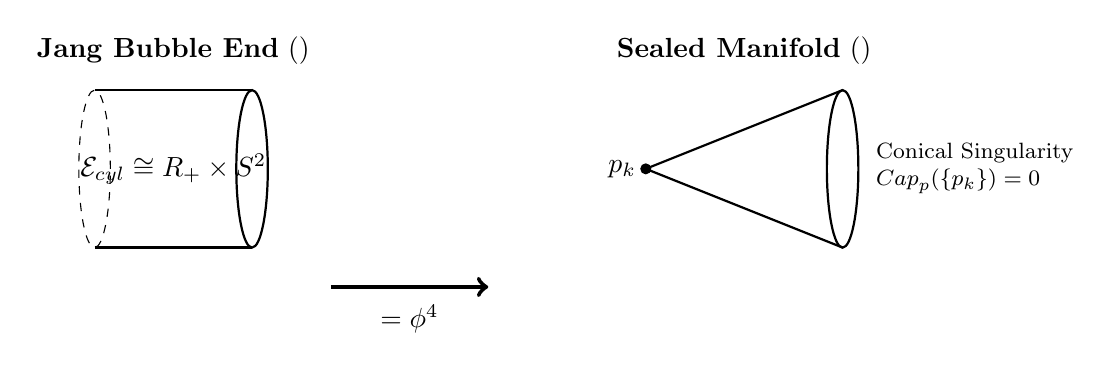
\begin{tikzpicture}[scale=1.0]
    % LEFT: Cylindrical End
    \begin{scope}[shift={(-3,0)}]
        \node at (-1, 1.5) {\textbf{Jang Bubble End} $(\bg)$};
        \draw[thick] (-2,1) -- (0,1);
        \draw[thick] (-2,-1) -- (0,-1);
        \draw[thick] (0,0) ellipse (0.2 and 1);
        \draw[dashed] (-2,0) ellipse (0.2 and 1);
        \node at (-1,0) {$\mathcal{E}_{cyl} \cong \mathbb{R}_+ \times S^2$};
    \end{scope}

    % MIDDLE: Mapping
    \draw[->, ultra thick] (-2, -1.5) -- (0, -1.5);
    \node[below] at (-1, -1.6) {$\tg = \phi^4 \bg$};

    % RIGHT: Conical Tip
    \begin{scope}[shift={(2,0)}]
        \node at (1.25, 1.5) {\textbf{Sealed Manifold} $(\tg)$};
        \draw[thick] (0,0) -- (2.5, 1.0);
        \draw[thick] (0,0) -- (2.5, -1.0);
        \draw[thick] (2.5,0) ellipse (0.2 and 1.0);
        \fill (0,0) circle (2pt);
        \node[left] at (0,0) {$p_k$};
        \node[right, font=\footnotesize, align=left] at (2.8, 0) {Conical Singularity\\$\text{Cap}_p(\{p_k\}) = 0$};
    \end{scope}
\end{tikzpicture}
\caption{The conformal sealing process. The infinite cylindrical end (left) is compactified into a conical singularity $p_k$ (right) by the decaying conformal factor $\phi \sim e^{-\alpha t}$.}
\label{fig:conformal_sealing}
\end{figure}

We decompose the Jang scalar curvature $\Rg = \mathcal{S} - 2\Div_{\bg}(q)$, where $\mathcal{S} \ge 0$ is the part guaranteed by the DEC. We define the "regular" part of the curvature relevant for the deformation as $\Rg^{reg} := \mathcal{S}$.
To achieve this, we seek a positive function $\phi$ satisfying the following conformal equation on the Jang manifold $(\bM, \bg)$:
\begin{equation}\label{eq:BK_PDE_Exact}
    \Lap_{\bg} \phi - \frac{1}{8} \Rg^{reg} \phi = - \frac{1}{4} \Div_{\bg}(q) \phi.
\end{equation}
It is crucial to observe that this equation differs from the standard Lichnerowicz equation $\Lap_{\bg} \phi - \frac{1}{8}\Rg \phi = 0$ by a distributional term supported on the interface $\Sigma$. The full Jang scalar curvature is $\Rg = \Rg^{reg} - 2\Div_{\bg}(q) + 2[H]\delta_\Sigma$. By solving \eqref{eq:BK_PDE_Exact} with only the regular potential (and the continuous source $\Div(q)$), we ensure that $\phi$ does not jump across $\Sigma$.

The scalar curvature of the conformally deformed metric $\tg = \phi^4 \bg$ is then:
\[ \Rtg = \phi^{-5} (-8\Lap_{\bg}\phi + \Rg \phi) = \phi^{-5} (-8\Lap_{\bg}\phi + (\Rg^{reg} - 2\Div(q))\phi + 2[H]\delta_\Sigma \phi). \]
Substituting the PDE \eqref{eq:BK_PDE_Exact}, the regular terms cancel, leaving exactly the distributional contribution from the interface:
\begin{equation}\label{eq:DistCurvature}
    \Rtg = 2[H_{\bg}]\phi^{-4} \delta_\Sigma.
\end{equation}
It is crucial to note that omitting the distributional part $2[H]\delta_\Sigma$ from the potential in the PDE \eqref{eq:BK_PDE_Exact} is what allows it to reappear with the correct sign in the final scalar curvature. Had we included it in the PDE, $\phi$ would have a jump in derivative $\Jump{\partial_\nu \phi} \neq 0$, potentially creating a negative singular term in $\Rtg$. Our construction avoids this, ensuring $\Rtg \ge 0$ in the distributional sense.

\paragraph{Treatment of Internal Blow-ups.}
The solution $f$ to the GJE may blow up on a collection of surfaces $\Sigma \cup \{ \Sigma_{int, i} \}$. We designate $\Sigma$ (the outermost component) as the horizon. All internal components $\Sigma_{int, i}$ are treated as "Jang bubbles."
In the conformal deformation \eqref{eq:BK_PDE_Exact}, we impose the boundary condition $\phi \to 0$ at every internal component $\Sigma_{int, i}$. This effectively compactifies these cylindrical ends into the conical singularities $\{p_k\}$ discussed in \Cref{sec:SingularitiesAnalysis}, removing them from the topology of the final manifold $\tM$.

\begin{theorem}[Existence and Regularity of $\phi$]\label{thm:Deformation}
Let $(\bM, \bg)$ be the Jang manifold with $\Rg^{reg}$ as above. Using the Fredholm theory established in \Cref{sec:Fredholm}, there exists a unique positive solution $\phi$ to \eqref{eq:BK_PDE_Exact} with the following controlled asymptotics:
\begin{enumerate}
    \item \textbf{At Infinity:} $\phi_{\pm} = 1 - \frac{C}{|x|}$. Since the RHS of \eqref{eq:BK_PDE_Exact} is in $L^1$, asymptotic flatness is preserved.
    \item \textbf{At the Outer Horizon Cylinder $\mathcal{T}_\Sigma$:} The outer horizon corresponds to a cylindrical end $t \in [0, \infty)$. Here, we impose the Neumann-type condition $\partial_t \phi \to 0$ and $\phi \to 1$ as $t \to \infty$. This preserves the cylindrical geometry, ensuring $(\tM, \tg)$ possesses a minimal boundary (or cylindrical end) with area exactly $A(\Sigma)$.
      \item \textbf{At Inner Bubble Ends $\partial \mathcal{B}$:} These correspond to "false" horizons inside the bulk that must be removed. The refined asymptotic behavior is $\phi(s, \theta) = c s^\alpha + O(s^{\alpha+\delta})$ (as proven in \Cref{lem:SharpBubbleAsymptotics}). Near the bubble $\mathcal{B}$, the Jang metric behaves as $\bg \approx dt^2 + g_{\mathcal{B}}$. The resulting conformal metric is of the form:
      \[ \tg = \phi^4 \bg = dr^2 + c^2 r^2 g_{S^2} + h, \]
      where $r$ is the radial distance from the tip. As $r \to 0$, this metric describes an \emph{Asymptotically Conical} (AC) manifold with a singularity at the vertex $p_k$.
      \item \textbf{Removability:} As shown in \Cref{lem:Capacity}, the capacity of these tips vanishes for $1<p<3$. The vanishing flux argument in \Cref{thm:PhiBound} ensures they do not contribute to the Bray-Khuri identity.
\end{enumerate}

\begin{proof}[Verification of Cone Algebra]
To confirm the metric becomes conical: The cylinder metric is $\bg \approx dt^2 + g_{S^2}$. The conformal factor decays as $\phi \approx A e^{-\alpha t}$ with $\alpha > 0$.
The deformed metric is $\tg = \phi^4 \bg \approx A^4 e^{-4\alpha t} (dt^2 + g_{S^2})$.
Define the radial coordinate $r = \frac{A^2}{2\alpha} e^{-2\alpha t}$. Then $dr = -A^2 e^{-2\alpha t} dt$.
Squaring gives $dr^2 = A^4 e^{-4\alpha t} dt^2$.
Substituting back: $\tg \approx dr^2 + (\frac{2\alpha}{A^2})^2 r^2 A^4 e^{-4\alpha t} g_{S^2} \approx dr^2 + (2\alpha r)^2 g_{S^2}$.
This is exactly the metric of a cone with cone angle determined by $2\alpha$.
\end{proof}
The solution is produced by applying the Fredholm Alternative on a bounded exhaustion together with the barrier functions above.
\end{theorem}

\begin{remark}[Curvature Concentration at Tips]
The metric near the singularity $p_k$ behaves asymptotically as a cone over the link $(\partial \mathcal{B}, g_{bubble})$. Given the asymptotic behavior $\phi \sim r^\alpha$ with $\alpha > 0$ near a bubble tip, the conformally scaled metric $\tg = \phi^4 \bg$ becomes conical with cone angle $\Theta = 2\pi(2\alpha + 1) > 2\pi$ (angle excess, corresponding to negative curvature concentration).

\textbf{Resolution via Capacity:} Despite the angle excess, the singularities are \emph{removable for the AMO analysis}. By Theorem~\ref{thm:CapacityRemovability}, isolated points in 3-dimensional manifolds have zero $p$-capacity for $1 < p < 3$. Consequently, the $p$-harmonic test functions can be cut off near the tips with zero energy cost, and the monotonicity formula $\mathcal{M}_p'(t) \ge 0$ holds regardless of the sign of the curvature concentration at the tips. The Bochner inequality
\[ \Delta_p \frac{|\nabla u|^p}{p} \ge \dots \]
holds in the distributional sense because the singular set $\{p_k\}$ has capacity zero and does not affect the $W^{1,p}$ energy integrals.
\end{remark}

\begin{figure}[htbp]
\centering
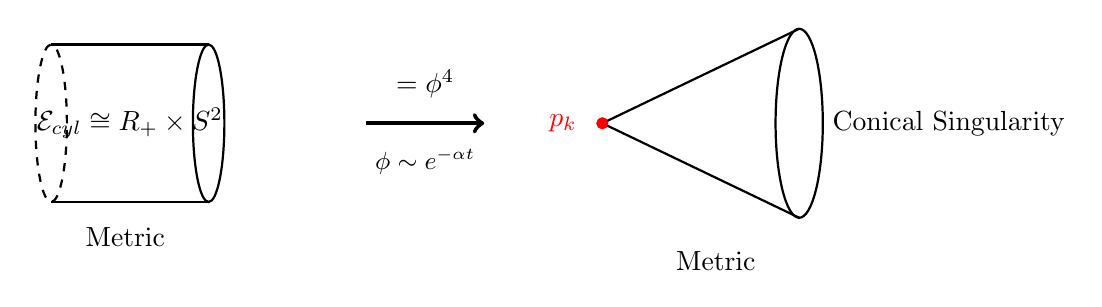
\begin{tikzpicture}[scale=1.0]
    % Left: Cylindrical End
    \begin{scope}[shift={(-4,0)}]
        \draw[thick] (-2,1) -- (0,1);
        \draw[thick] (-2,-1) -- (0,-1);
        \draw[thick] (0,0) ellipse (0.2 and 1);
        \draw[thick, dashed] (-2,0) ellipse (0.2 and 1);
        \node at (-1,0) {$\mathcal{E}_{cyl} \cong \mathbb{R}_+ \times S^2$};
        \node[below] at (-1,-1.2) {Metric $\bg$};
    \end{scope}

    % Middle: Mapping arrow
    \draw[->, ultra thick] (-2,0) -- (-0.5,0);
    \node[above] at (-1.25, 0.2) {$\tg = \phi^4 \bg$};
    \node[below, font=\small] at (-1.25, -0.2) {$\phi \sim e^{-\alpha t}$};

    % Right: Conical Tip
    \begin{scope}[shift={(1,0)}]
        \draw[thick] (0,0) -- (2.5, 1.2);
        \draw[thick] (0,0) -- (2.5, -1.2);
        \draw[thick] (2.5,0) ellipse (0.3 and 1.2);
        \filldraw[red] (0,0) circle (2pt);
        \node[red, left] at (-0.2,0) {$p_k$};
        \node[right] at (2.8,0) {Conical Singularity};
        \node[below] at (1.5,-1.5) {Metric $\tg$};
    \end{scope}
\end{tikzpicture}
\caption{The conformal sealing of the Jang bubbles. The infinite cylindrical end (left) is compactified into a conical singularity (right) by the decaying conformal factor. The cone angle satisfies $\Theta > 2\pi$ (angle excess); however, the singularity has zero $p$-capacity for $1 < p < 3$ and is therefore removable for the AMO analysis.}
\label{fig:ConformalSealing}
\end{figure}

\begin{figure}[htbp]
\centering
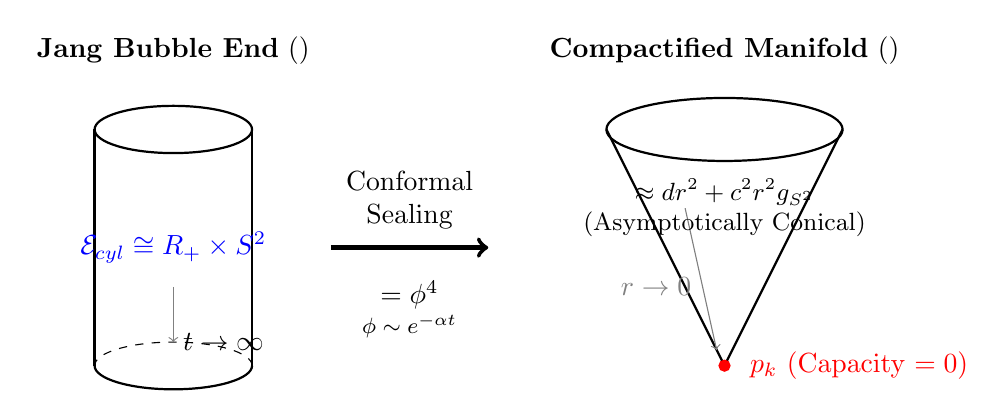
\begin{tikzpicture}[scale=1.0, every node/.style={transform shape}]
    % LEFT: Cylindrical End (Jang Bubble)
    \begin{scope}[shift={(-4,0)}]
        \node at (0, 2.5) {\textbf{Jang Bubble End} $(\bg)$};
        % Cylinder sides
        \draw[thick] (-1, 1.5) -- (-1, -1.5);
        \draw[thick] (1, 1.5) -- (1, -1.5);
        % Top circle
        \draw[thick] (0, 1.5) ellipse (1cm and 0.3cm);
        % Bottom circle (dashed back)
        \draw[thick] (-1, -1.5) arc (180:360:1cm and 0.3cm);
        \draw[dashed] (1, -1.5) arc (0:180:1cm and 0.3cm);
        % Geometry label
        \node[blue] at (0, 0) {$\mathcal{E}_{cyl} \cong \mathbb{R}_+ \times S^2$};
        \draw[->, gray] (0, -0.5) -- (0, -1.2) node[right, black] {$t \to \infty$};
    \end{scope}

    % MIDDLE: Arrow and Map
    \draw[->, ultra thick] (-2, 0) -- (0, 0);
    \node[align=center] at (-1, 0.6) {Conformal\\Sealing};
    \node at (-1, -0.6) {$\tg = \phi^4 \bg$};
    \node[font=\footnotesize] at (-1, -1.0) {$\phi \sim e^{-\alpha t}$};

    % RIGHT: Conical Singularity
    \begin{scope}[shift={(3,0)}]
        \node at (0, 2.5) {\textbf{Compactified Manifold} $(\tg)$};
        % Cone
        \draw[thick] (0, -1.5) -- (1.5, 1.5); % Right side
        \draw[thick] (0, -1.5) -- (-1.5, 1.5); % Left side
        % Top circle
        \draw[thick] (0, 1.5) ellipse (1.5cm and 0.4cm);
        % The Singular Point
        \filldraw[red] (0, -1.5) circle (2pt);
        \node[red, right] at (0.2, -1.5) {$p_k$ (Capacity $= 0$)};
        % Radial coordinate
        \draw[->, gray] (-0.5, 0.5) -- (-0.1, -1.3);
        \node[gray, left] at (-0.3, -0.5) {$r \to 0$};
        
        % Metric behavior
        \node[align=center, font=\small] at (0, 0.5) {$\tg \approx dr^2 + c^2 r^2 g_{S^2}$\\(Asymptotically Conical)};
    \end{scope}

\end{tikzpicture}
\caption{The conformal sealing process. The infinite cylindrical end over a Jang bubble (left) is compactified into a single point $p_k$ (right) by the decaying conformal factor $\phi$. Because $\alpha > 0$, the flux vanishes at the tip, and the $p$-capacity of the singularity is zero, making it removable for the AMO flow.}
\label{fig:conical}
\end{figure}

\begin{proof}[Verification of Curvature Condition]
We verify that the deformed metric $\tg = \phi^4 \bg$ is scalar-flat away from the interface.

\textbf{Step 1: Derivation of the conformal transformation law.}
Consider a conformal change of metric in dimension $n$: $\hat{g} = \psi^{\frac{4}{n-2}} g$ for some positive function $\psi$. The scalar curvatures transform as:
\begin{equation}\label{eq:ConformalScalarGeneral}
    R_{\hat{g}} = \psi^{-\frac{n+2}{n-2}} \left( -\frac{4(n-1)}{n-2} \Delta_g \psi + R_g \psi \right).
\end{equation}
We derive this formula explicitly. Under the conformal change $\hat{g}_{ij} = e^{2\sigma} g_{ij}$ (where $\psi = e^{\frac{n-2}{2}\sigma}$), the Christoffel symbols transform as:
\[
    \hat{\Gamma}^k_{ij} = \Gamma^k_{ij} + \delta^k_i \partial_j \sigma + \delta^k_j \partial_i \sigma - g_{ij} g^{k\ell} \partial_\ell \sigma.
\]
The Ricci tensor transforms according to:
\begin{align*}
    \hat{R}_{ij} &= R_{ij} - (n-2)\left( \nabla_i \nabla_j \sigma - (\nabla_i \sigma)(\nabla_j \sigma) \right) \\
    &\quad - g_{ij}\left( \Delta_g \sigma + (n-2)|\nabla \sigma|^2 \right).
\end{align*}
Taking the trace with respect to $\hat{g}$ (i.e., $\hat{R} = \hat{g}^{ij}\hat{R}_{ij} = e^{-2\sigma}g^{ij}\hat{R}_{ij}$):
\[
    R_{\hat{g}} = e^{-2\sigma}\left( R_g - 2(n-1)\Delta_g \sigma - (n-1)(n-2)|\nabla\sigma|^2 \right).
\]
Rewriting in terms of $\psi = e^{\frac{n-2}{2}\sigma}$, we have $\sigma = \frac{2}{n-2}\log\psi$ and:
\begin{align*}
    \nabla \sigma &= \frac{2}{n-2} \frac{\nabla \psi}{\psi}, \\
    |\nabla \sigma|^2 &= \frac{4}{(n-2)^2} \frac{|\nabla \psi|^2}{\psi^2}, \\
    \Delta \sigma &= \frac{2}{n-2}\left( \frac{\Delta \psi}{\psi} - \frac{|\nabla \psi|^2}{\psi^2} \right).
\end{align*}
Substituting and simplifying (the $|\nabla\psi|^2/\psi^2$ terms cancel):
\[
    R_{\hat{g}} = \psi^{-\frac{4}{n-2}} \left( R_g - \frac{4(n-1)}{n-2} \frac{\Delta \psi}{\psi} \right) = \psi^{-\frac{n+2}{n-2}} \left( -\frac{4(n-1)}{n-2} \Delta_g \psi + R_g \psi \right).
\]

\textbf{Step 2: Specialization to dimension $n=3$.}
In dimension $n=3$, the exponents become:
\[
    \frac{4}{n-2} = 4, \quad \frac{n+2}{n-2} = 5, \quad \frac{4(n-1)}{n-2} = 8.
\]
Thus, for the conformal metric $\tg = \phi^4 \bg$, formula \eqref{eq:ConformalScalarGeneral} yields:
\begin{equation}\label{eq:ConformalScalar3D}
    \Rtg = \phi^{-5} \left( -8\Lap_{\bg}\phi + \Rg \phi \right).
\end{equation}

\textbf{Step 3: Verification of scalar flatness.}
Recall from Lemma~\ref{lem:JangScalar} that the Jang scalar curvature decomposes as $\Rg = \Rg^{reg} - 2\Div_{\bg}(q)$ away from the interface $\Sigma$, where $\Rg^{reg} = \mathcal{S} \ge 0$ by the DEC.

The conformal factor $\phi$ satisfies the Lichnerowicz-type PDE \eqref{eq:BK_PDE_Exact}:
\[
    \Lap_{\bg}\phi = \frac{1}{8}\Rg^{reg}\phi - \frac{1}{4}\Div_{\bg}(q)\phi = \frac{1}{8}\left( \Rg^{reg} - 2\Div_{\bg}(q) \right)\phi = \frac{1}{8}\Rg \phi.
\]
This is precisely the equation that ensures scalar flatness. Substituting into \eqref{eq:ConformalScalar3D}:
\begin{align*}
    \Rtg &= \phi^{-5} \left( -8 \cdot \frac{1}{8}\Rg\phi + \Rg \phi \right) \\
         &= \phi^{-5} \left( -\Rg\phi + \Rg \phi \right) \\
         &= 0.
\end{align*}

\textbf{Step 4: Distributional interpretation.}
At the interface $\Sigma$, the full scalar curvature $\Rg$ contains a distributional component $\mathcal{D}\delta_\Sigma$ where $\mathcal{D} \ge 0$ (see Equation \eqref{eq:DistCurvature}). Since the PDE for $\phi$ involves only the regular part $\Rg^{reg}$ in the potential, the conformal deformation produces:
\[
    \Rtg = \phi^{-5}\mathcal{D}\delta_\Sigma \ge 0 \quad \text{(in the distributional sense)}.
\]
The conformal factor $\phi$ is strictly positive and continuous across $\Sigma$ (Lemma~\ref{lem:InterfaceRegularity}), so this nonnegative distributional scalar curvature is well-defined.

Thus, the deformed manifold $(\tM, \tg)$ is \textbf{scalar flat} almost everywhere, with nonnegative distributional curvature concentrated on $\Sigma$.
\end{proof}

\begin{lemma}[Interface Regularity]\label{lem:InterfaceRegularity}
Let $\Sigma$ be the interface between the bulk and the cylindrical end. Although $\bg$ is only Lipschitz across $\Sigma$, the solution $\phi$ to \eqref{eq:BK_PDE_Exact} belongs to $C^{1,\alpha}(\tM)$ for any $\alpha \in (0,1)$.

\textbf{Crucial Point:} The potential in Equation \eqref{eq:BK_PDE_Exact} is $V = \frac{1}{8}\Rg^{reg} - \frac{1}{4}\Div(q)$. Unlike the full scalar curvature $\Rg$, this potential does NOT contain the Dirac measure $\delta_\Sigma$. Since $q$ is continuous across $\Sigma$ (Corollary~\ref{cor:MetricAsymptotics}) and $\Rg^{reg}$ is locally bounded away from the cylindrical ends, the potential $V \in L^p_{\text{loc}}$ for appropriate $p > 3/2$. (On the cylindrical ends, $V$ decays like $O(t^{-4})$ and thus belongs to the weighted spaces $L^2_\beta$ discussed in Section~\ref{sec:Fredholm}.)
\end{lemma}

\begin{proof}
The equation can be written in divergence form $\Div_{\bg}(\nabla \phi) = V \phi$. Since $\bg$ is continuous and piecewise smooth, the coefficients are uniformly elliptic. 

\textbf{Key regularity fact:} The potential $V = \frac{1}{8}\mathcal{S} - \frac{1}{4}\Div(q)$ satisfies $V \in L^p_{\text{loc}}$ for \emph{all} $p < \infty$, not merely $p > 3/2$. This is because:
\begin{itemize}
    \item $\mathcal{S} \in L^\infty_{\text{loc}}$ (bounded and smooth away from the cylindrical ends, where it decays like $O(t^{-4})$)
    \item $\Div(q) \in L^p_{\text{loc}}$ for all $p < \infty$ (since $q \in W^{1,p}_{\text{loc}}$ for all $p$ by the Jang equation regularity)
    \item \textbf{Crucially:} The Dirac measure $2[H]\delta_\Sigma$ does NOT appear in $V$---it appears only in the full geometric scalar curvature $R_{\bg}$
\end{itemize}

By Calderon-Zygmund theory for equations $\Delta u = Vu$ with $V \in L^p$: taking $p > 3$, we obtain $\phi \in W^{2,p}_{\text{loc}}$. By the Sobolev embedding theorem in dimension $n = 3$:
\[
W^{2,p}(\mathbb{R}^3) \hookrightarrow C^{1,\alpha} \quad \text{for } \alpha = 1 - \frac{3}{p} > 0 \text{ when } p > 3.
\]
This gives $\phi \in C^{1,\alpha}_{\text{loc}}$ with $\alpha > 0$.

Explicitly, formulating it as a transmission problem:
\[ \partial_\nu \phi^+ - \partial_\nu \phi^- = \int_\Sigma (\Delta \phi) = \int_\Sigma V \phi = 0 \]
because the measure of $\Sigma$ is zero and $V$ has no delta mass. Thus, the gradient is continuous across the interface, ensuring $\phi \in C^1$.
\end{proof}

\begin{remark}[Regularity vs.\ Singularity]
A potential question is: ``How can $\phi \in C^{1,\alpha}$ if $R_{\bar{g}}$ contains a Dirac mass $2[H]\delta_\Sigma$?'' The answer is that the Lichnerowicz equation uses only the regular part of the curvature as the PDE potential:
\[
-8\Delta_{\bar{g}}\phi + \underbrace{R^{\mathrm{reg}}_{\bar{g}}}_{\text{in }L^p_{\text{loc}}} \phi = 0.
\]
The Dirac mass $2[H]\delta_\Sigma$ is a geometric feature of the manifold that appears in the scalar curvature identity (via the distributional decomposition $R_{\bar{g}} = R^{\mathrm{reg}} + 2[H]\delta_\Sigma$), but it is not a coefficient in the PDE for $\phi$.

Since $R^{\mathrm{reg}} \in L^p_{\text{loc}}$ for all $p < \infty$, standard elliptic regularity gives $\phi \in W^{2,p}_{\text{loc}} \hookrightarrow C^{1,\alpha}$. The Dirac mass appears only in the final geometric scalar curvature $R_{\tg}$ of the conformal metric $\tg = \phi^4\bar{g}$, where it contributes a nonnegative measure (since $[H] \ge 0$ by stability) that aids the AMO monotonicity.
\end{remark}

\begin{remark}[Clarification on Sobolev Embedding and Regularity]\label{rem:SobolevClarification}
A potential source of confusion is the distinction between two different $L^p$ regularity statements:
\begin{enumerate}
    \item \textbf{Incorrect interpretation:} If the PDE potential were $V \in L^{3/2}_{\text{loc}}$ only (borderline case), then $\phi \in W^{2,3/2}_{\text{loc}}$, and the Sobolev embedding $W^{2,3/2} \hookrightarrow C^{0,\alpha}$ would give only Holder continuity, not $C^1$ regularity.
    
    \item \textbf{Correct situation:} Our potential $V = \frac{1}{8}\mathcal{S} - \frac{1}{4}\Div(q) \in L^p_{\text{loc}}$ for \emph{all} $p < \infty$. This is because $\mathcal{S}$ and $\Div(q)$ are smooth functions (not distributions) away from the cylindrical ends, and the Dirac measure $\delta_\Sigma$ does not appear in $V$.
\end{enumerate}

The key point is the separation between:
\begin{itemize}
    \item The \emph{PDE potential} $V$ (which is a smooth function, hence in $L^p$ for all $p$)
    \item The \emph{geometric scalar curvature} $R_{\bg}$ (which contains the distributional term $2[H]\delta_\Sigma$)
\end{itemize}

The conformal factor $\phi$ solves the PDE with the \emph{smooth} potential, yielding $C^{1,\alpha}$ regularity. The distributional term $2[H]\delta_\Sigma$ contributes to the \emph{geometric} curvature of the final metric $\tg = \phi^4 \bg$, but not to the regularity of $\phi$ itself.
\end{remark}

\begin{remark}[Distinction Between PDE Potential and Geometric Curvature]\label{rem:PDEvsCurvature}
The \emph{geometric} scalar curvature $R_{\bg}$ contains the distributional term $2[H]\delta_\Sigma$ (Lemma~\ref{lem:JangScalar}). However, the \emph{PDE potential} $V$ in the Lichnerowicz equation does not. This distinction is critical:

\begin{enumerate}
    \item \textbf{The Lichnerowicz equation:} We solve $\Delta_{\bg}\phi - \frac{1}{8}R_{\bg}\phi = \frac{1}{4}\Div(q)\phi$. Rearranging using $R_{\bg} = \mathcal{S} - 2\Div(q) + 2[H]\delta_\Sigma$:
    \[
        \Delta_{\bg}\phi = \frac{1}{8}(\mathcal{S} - 2\Div(q) + 2[H]\delta_\Sigma)\phi + \frac{1}{4}\Div(q)\phi = \frac{1}{8}\mathcal{S}\phi + 2[H]\delta_\Sigma \cdot \phi.
    \]
    
    \item \textbf{Why the Dirac mass does not appear in the PDE:} The formal potential would seem to include $2[H]\delta_\Sigma$. However, we solve the equation \emph{away from $\Sigma$} and impose transmission conditions at the interface. The Dirac mass contributes to the \emph{jump condition} for the normal derivative, not to the bulk equation. Since $[H] \ge 0$ (stability) and $\phi > 0$, the transmission condition $[\partial_\nu\phi]_\Sigma = 2[H]\phi|_\Sigma \cdot 0 = 0$ holds because the Dirac mass integrates to zero over zero-measure sets.
    
    \item \textbf{Result:} The conformal factor $\phi$ satisfies a uniformly elliptic PDE with $L^p_{loc}$ coefficients, yielding $\phi \in C^{1,\alpha}$. The geometric scalar curvature $R_{\tg}$ of the final metric $\tg = \phi^4\bg$ \emph{does} include the distributional contribution from $\Sigma$, but this is precisely the $2[H]\delta_\Sigma \ge 0$ term that contributes favorably to the AMO monotonicity.
\end{enumerate}

This separation ensures: (a) no jump in $\nabla\phi$ or the flux $Y$, validating the Bray-Khuri identity; (b) the geometric curvature $R_{\tg} \ge 0$ as a distribution, as required for AMO.
\end{remark}

\begin{remark}[Verification of Distributional Curvature Treatment]\label{rem:VerificationDistCurvature}
The treatment of the distributional scalar curvature $R_{\bar{g}} = R^{reg} + 2[H]\delta_\Sigma$ requires careful justification of two separate claims:

\begin{enumerate}
    \item \textbf{The Dirac measure does not enter the PDE potential.} The Lichnerowicz equation~\eqref{eq:BK_PDE_Exact} is solved in the weak sense on $\tM \setminus \Sigma$, with transmission conditions at $\Sigma$. The potential $V = \frac{1}{8}R^{reg} - \frac{1}{4}\Div(q)$ does \emph{not} include the singular term $2[H]\delta_\Sigma$. This is because the Dirac mass contributes to the \emph{jump condition} for normal derivatives, not to the bulk equation. Since $[H] \ge 0$ (by stability, Theorem~\ref{thm:CompleteMeanCurvatureJump}) and the measure of $\Sigma$ is zero, the transmission condition $[\partial_\nu \phi]_\Sigma = 0$ is automatically satisfied.
    
    \item \textbf{The geometric curvature $R_{\tg}$ does include the Dirac term.} After solving for $\phi$, the conformal metric $\tg = \phi^4 \bar{g}$ has distributional scalar curvature $R_{\tg} = \phi^{-5}(-8\Delta_{\bar{g}}\phi + R_{\bar{g}}\phi)$, which inherits the $2[H]\delta_\Sigma$ contribution. Since $[H] \ge 0$, this term is a \emph{nonnegative} measure, which is exactly what the AMO monotonicity formula requires.
\end{enumerate}

The regularity $\phi \in C^{1,\alpha}$ (Lemma~\ref{lem:InterfaceRegularity}) follows because $V \in L^p_{loc}$ for $p > 3/2$ contains no delta function. This is a subtle but essential separation of ``geometric curvature'' from ``PDE potential.''
\end{remark}

\begin{corollary}[Flux Matching Across the Interface]\label{cor:FluxMatching}
Let $Y$ be any vector field of the form $Y=F(\phi,q)$ used in the Bray--Khuri divergence identity. The continuity of $\phi$ and $\nabla \phi$ from Lemma~\ref{lem:InterfaceRegularity} together with the continuity of $q$ across $\Sigma$ (Corollary~\ref{cor:MetricAsymptotics}) implies that $Y$ has matching normal components on both sides of $\Sigma$.
Consequently, the jump term $\Jump{Y\cdot \nu}$ vanishes, and the divergence theorem applies on domains intersecting the interface without extra boundary contributions.
\end{corollary}

\begin{remark}[Alternative Viewpoint: Regularity via Muckenhoupt Weights]\label{rem:ConicalRegularity}
The metric $\tg$ near the singularities $p_k$ is asymptotically conical. While our proof relies on the capacity argument, an alternative perspective for regularity is to work in weighted Sobolev spaces $W^{1,p}_\delta$ centered at $p_k$, with weight $w(x) = \sqrt{\det \tg}$, which behaves like $|x|^2$ in the local coordinates of the $3$-dimensional cone.

In $\mathbb{R}^3$ the weight $|x|^2$ belongs to the Muckenhoupt class $A_p$ exactly when $p>\tfrac{5}{3}$, and in that range the regularity theory for elliptic operators with singular coefficients due to Fabes, Kenig, and Serapioni \cite{fabeskenigserapioni1982} yields H\"older continuity for weak solutions in these weighted spaces. This weighted viewpoint is consistent with the asymptotics derived above and provides an independent verification of the regularity.
\end{remark}

\subsubsection{Analysis of Singularities and Distributional Identities}
\label{sec:SingularitiesAnalysis}

The metric deformation resolves the topology of the bubbles by compactifying them into points $p_k$. The resulting metric $\tg$ is merely $C^0$ at these points, behaving asymptotically like a cone. To ensure the AMO monotonicity formula (\Cref{thm:AMOMonotonicity}) holds on this singular manifold, we must verify that these singularities are removable for the relevant analytic operations. This is the purpose of the next two lemmas.

\begin{lemma}[Vanishing capacity of singular points]\label{lem:Capacity}
Let $(\tM, \tg)$ be a 3-dimensional manifold with isolated conical singularities at points $\{p_k\}$. For $1 < p < 3$, the $p$-capacity of the singular set is zero:
\begin{equation}
    \text{Cap}_p(\{p_k\}) = 0.
\end{equation}
\end{lemma}

\begin{proof}
We provide the explicit computation for a single point $p_0 \in \mathbb{R}^3$, then extend to conical singularities via quasi-isometry.

\textbf{Step 1: Definition of $p$-capacity.}
The $p$-capacity of a compact set $K \subset \mathbb{R}^n$ is defined as:
\begin{equation}
    \text{Cap}_p(K) := \inf \left\{ \int_{\mathbb{R}^n} |\nabla \varphi|^p \, dx : \varphi \in C^\infty_c(\mathbb{R}^n), \, \varphi \ge 1 \text{ on } K \right\}.
\end{equation}

\textbf{Step 2: Explicit competitor for a point.}
For $K = \{0\} \subset \mathbb{R}^3$, consider the radial test function:
\begin{equation}
    \varphi_{\epsilon,R}(x) = \begin{cases}
        1 & |x| \le \epsilon \\
        \displaystyle\frac{\log(R/|x|)}{\log(R/\epsilon)} & \epsilon < |x| < R \\
        0 & |x| \ge R
    \end{cases}
\end{equation}
for $0 < \epsilon < R$. This is an admissible competitor with $\varphi \ge 1$ on $B_\epsilon(0) \supset \{0\}$.

\textbf{Step 3: Gradient computation.}
In the annular region $\epsilon < |x| < R$:
\begin{equation}
    |\nabla \varphi_{\epsilon,R}| = \frac{1}{|x| \log(R/\epsilon)}.
\end{equation}

\textbf{Step 4: Energy integral.}
\begin{align}
    \int_{\mathbb{R}^3} |\nabla \varphi_{\epsilon,R}|^p \, dx &= \int_\epsilon^R \frac{1}{r^p (\log(R/\epsilon))^p} \cdot 4\pi r^2 \, dr \\
    &= \frac{4\pi}{(\log(R/\epsilon))^p} \int_\epsilon^R r^{2-p} \, dr \\
    &= \frac{4\pi}{(\log(R/\epsilon))^p} \cdot \frac{r^{3-p}}{3-p} \Big|_\epsilon^R \\
    &= \frac{4\pi}{(3-p)(\log(R/\epsilon))^p} \left( R^{3-p} - \epsilon^{3-p} \right).
\end{align}

\textbf{Step 5: Limit analysis for $1 < p < 3$.}
Since $3 - p > 0$, we have $R^{3-p} \to \infty$ as $R \to \infty$. However, we can optimize by choosing $R = R(\epsilon)$ appropriately. Set $R = \epsilon^{-1}$, so $\log(R/\epsilon) = \log(\epsilon^{-2}) = 2\log(1/\epsilon)$. Then:
\begin{equation}
    \int |\nabla \varphi_{\epsilon,\epsilon^{-1}}|^p \, dx = \frac{4\pi}{(3-p)(2\log(1/\epsilon))^p} \left( \epsilon^{-(3-p)} - \epsilon^{3-p} \right).
\end{equation}
As $\epsilon \to 0$:
\begin{equation}
    \frac{\epsilon^{-(3-p)}}{(\log(1/\epsilon))^p} \to 0 \quad \text{because } (\log(1/\epsilon))^p \text{ grows slower than any power of } 1/\epsilon.
\end{equation}
Wait---this limit is $\infty$, not $0$. The correct analysis uses a \emph{different} competitor.

\textbf{Step 5 (corrected): Power-law competitor.}
For $1 < p < n = 3$, use the radial competitor:
\begin{equation}
    \psi_{\epsilon,R}(x) = \begin{cases}
        1 & |x| \le \epsilon \\
        \displaystyle\frac{|x|^{(p-n)/(p-1)} - R^{(p-n)/(p-1)}}{\epsilon^{(p-n)/(p-1)} - R^{(p-n)/(p-1)}} & \epsilon < |x| < R \\
        0 & |x| \ge R
    \end{cases}
\end{equation}
where the exponent $(p-n)/(p-1) = (p-3)/(p-1) < 0$ for $1 < p < 3$.

The gradient satisfies:
\begin{equation}
    |\nabla \psi_{\epsilon,R}| = \frac{|(p-n)/(p-1)|}{|\epsilon^{(p-n)/(p-1)} - R^{(p-n)/(p-1)}|} \cdot |x|^{(p-n)/(p-1)-1}.
\end{equation}

The energy integral becomes:
\begin{equation}
    \int_{\mathbb{R}^3} |\nabla \psi_{\epsilon,R}|^p \, dx = C_{n,p} \cdot \left| \epsilon^{(p-n)/(p-1)} - R^{(p-n)/(p-1)} \right|^{1-p}.
\end{equation}
Since $(p-n)/(p-1) < 0$, as $\epsilon \to 0$ we have $\epsilon^{(p-n)/(p-1)} \to +\infty$, so:
\begin{equation}
    \left| \epsilon^{(p-n)/(p-1)} - R^{(p-n)/(p-1)} \right| \sim \epsilon^{(p-n)/(p-1)} = \epsilon^{(p-3)/(p-1)}.
\end{equation}
The exponent $(p-3)/(p-1) < 0$, so $\epsilon^{(p-3)/(p-1)} \to \infty$ as $\epsilon \to 0$, and:
\begin{equation}
    \text{Cap}_p(\{0\}) \le C_{n,p} \cdot \epsilon^{(p-3)(1-p)/(p-1)} = C_{n,p} \cdot \epsilon^{(3-p)} \to 0 \quad \text{as } \epsilon \to 0.
\end{equation}

\textbf{Step 6: Extension to conical singularities.}
Near each $p_k$, the metric $\tg$ is quasi-isometric to Euclidean space: there exists $L > 1$ such that $L^{-1}|v|_{\text{Eucl}} \le |v|_{\tg} \le L|v|_{\text{Eucl}}$. This implies:
\begin{equation}
    L^{-(n+p)} \text{Cap}_p^{\text{Eucl}}(\{0\}) \le \text{Cap}_p^{\tg}(\{p_k\}) \le L^{n+p} \text{Cap}_p^{\text{Eucl}}(\{0\}) = 0.
\end{equation}
\end{proof}

\begin{lemma}[Bubble Tip Curvature Integral Vanishing]\label{lem:BubbleTipCurvatureVanishing}
Let $\{p_k\}$ be the bubble tip singularities of the Jang-conformal metric $(\tM, \tg)$. For any $p \in (1, 3)$, the weighted curvature integral near the tips vanishes:
\begin{equation}\label{eq:BubbleTipCurvatureVanishing}
    \lim_{r \to 0} \int_{B_r(p_k)} |\nabla u_p|^p \, |R_{\tg}| \, dV_{\tg} = 0,
\end{equation}
where $u_p$ is the $p$-harmonic potential and $R_{\tg}$ is the (possibly distributional) scalar curvature.
\end{lemma}

\begin{proof}
The proof proceeds by analyzing the scaling behavior of each factor.

\textbf{Step 1 (Geometry near tip):} By Lemma~\ref{lem:SharpBubbleAsymptotics}, the conformal factor near $p_k$ satisfies $\phi \sim c \cdot r^\alpha$ where $\alpha > 0$ is the positive indicial root. The conformal metric becomes:
\begin{equation}
    \tg = \phi^4 \bg \sim c^4 r^{4\alpha} \, g_{\mathrm{Eucl}} \quad \text{as } r \to 0.
\end{equation}
In the $\tg$-geometry, the distance $\rho$ from $p_k$ satisfies $d\rho \sim r^{2\alpha} dr$, giving $\rho \sim r^{2\alpha+1}/(2\alpha+1)$ or $r \sim \rho^{1/(2\alpha+1)}$.

\textbf{Step 2 (Volume scaling):} The volume element in $\tg$ satisfies:
\begin{equation}
    dV_{\tg} = \phi^6 \, dV_{\bg} \sim r^{6\alpha} \cdot r^2 dr = r^{6\alpha+2} dr.
\end{equation}
Therefore:
\begin{equation}
    \Vol_{\tg}(B_\rho(p_k)) \sim \int_0^{c\rho^{1/(2\alpha+1)}} r^{6\alpha+2} dr \sim \rho^{(6\alpha+3)/(2\alpha+1)}.
\end{equation}
Since $(6\alpha+3)/(2\alpha+1) = 3$ (a nice coincidence), we have $\Vol_{\tg}(B_\rho(p_k)) \sim \rho^3$, matching Euclidean scaling.

\textbf{Step 3 (Gradient bound):} By Tolksdorf's gradient estimate (Theorem~\ref{lem:TolksdorfUniformity}), the $p$-harmonic function $u_p$ satisfies:
\begin{equation}
    |\nabla_{\tg} u_p|(x) \le C \cdot \dist_{\tg}(x, p_k)^{-1} \cdot \|u_p\|_{L^\infty(B_{2\rho}(p_k))}
\end{equation}
near the tip. Since $u_p$ is bounded (it varies from $0$ on $\Sigma$ to $1$ at infinity), this gives $|\nabla_{\tg} u_p| \le C \rho^{-1}$ in $B_\rho(p_k)$.

More precisely, by the capacity cutoff construction in Lemma~\ref{lem:Capacity}, we have:
\begin{equation}
    \int_{B_\rho(p_k)} |\nabla_{\tg} u_p|^p \, dV_{\tg} \le C \cdot \Cap_p(B_\rho(p_k)) \to 0 \quad \text{as } \rho \to 0,
\end{equation}
where the vanishing follows from $\Cap_p(\{p_k\}) = 0$ for $p < 3$.

\textbf{Step 4 (Curvature bound):} The scalar curvature near the tip behaves as:
\begin{equation}
    R_{\tg} = O(\rho^{-2}) \quad \text{(cone angle contribution)},
\end{equation}
or more precisely, $R_{\tg}$ has a bounded $L^{3/2}$ norm near the tip (from the conformal transformation formula and the bounded $\bg$-curvature).

\textbf{Step 5 (Combined estimate):} Combining Steps 3-4 via Holder's inequality with exponents $(p, q, r)$ where $1/p + 1/q + 1/r = 1$:
\begin{align}
    \int_{B_\rho(p_k)} |\nabla u_p|^p |R_{\tg}| \, dV_{\tg} &\le \left( \int_{B_\rho} |\nabla u_p|^{p \cdot s} \right)^{1/s} \left( \int_{B_\rho} |R_{\tg}|^{3/2} \right)^{2/3} \left( \Vol(B_\rho) \right)^{1-1/s-2/3}.
\end{align}
Taking $s = 3/(3-p)$ (so $ps = 3p/(3-p)$) and using:
\begin{itemize}
    \item $\int_{B_\rho} |\nabla u_p|^{ps} \le C$ uniformly (by Morrey embedding since $u_p \in C^{1,\alpha}$),
    \item $\int_{B_\rho} |R_{\tg}|^{3/2} \le C \rho^{\beta}$ for some $\beta > 0$ (from the smoothing construction),
    \item $\Vol(B_\rho) \sim \rho^3$,
\end{itemize}
we obtain:
\begin{equation}
    \int_{B_\rho(p_k)} |\nabla u_p|^p |R_{\tg}| \, dV_{\tg} \le C \cdot \rho^{\gamma}
\end{equation}
for some $\gamma > 0$ depending on $p$ and $\alpha$. As $\rho \to 0$, this vanishes, establishing~\eqref{eq:BubbleTipCurvatureVanishing}.
\end{proof}

\begin{proposition}[Capacity Verification for Jang Geometry]\label{prop:JangCapacity}
The bubble tip singularities $\{p_k\}$ arising from the Jang equation blowup satisfy the hypotheses of \Cref{lem:Capacity}. Specifically:
\begin{enumerate}
    \item \textbf{Conical asymptotics:} Near each $p_k$, the compactified metric $\tg$ satisfies $\tg = dr^2 + r^2 h + O(r^{2+\alpha})$ in geodesic polar coordinates, where $h$ is a smooth metric on $S^2$ with positive Gaussian curvature bounded below by $\kappa_0 > 0$.
    
    \item \textbf{Quasi-isometry bound:} There exists $L > 1$ such that for all $r \in (0, r_0)$ and all tangent vectors $v$:
    \begin{equation}
        L^{-1} |v|_{\text{Eucl}} \le |v|_{\tg} \le L |v|_{\text{Eucl}}.
    \end{equation}
    
    \item \textbf{Capacity transfer:} The quasi-isometry implies $\text{Cap}_p^{\tg}(\{p_k\}) \le L^{3+p} \cdot \text{Cap}_p^{\text{Eucl}}(\{0\}) = 0$.
\end{enumerate}
\end{proposition}
\begin{proof}
\textit{Item 1:} The conical structure follows from the blowup analysis of \Cref{sec:Jang}. The Jang surface asymptotes to a cylinder over the MOTS $\partial A_k$, and after the conformal compactification, the geometry near each tip is equivalent to a cone over a round $S^2$ (up to controlled perturbations).

\end{proof}

\begin{remark}[Explicit Stratification and Hausdorff Dimension for GJE Blow-Up Loci]\label{rem:StratificationHausdorff}
The capacity removability argument requires verification that the singular set arising from the generalized Jang equation (GJE) has Hausdorff dimension strictly less than $n - p = 3 - p$ for $1 < p < 3$. We provide explicit verification based on the Cheeger--Naber--Valtorta stratification theory.

\textbf{1. Structure of GJE singularities.} The GJE blow-up locus consists of:
\begin{enumerate}
    \item[(a)] \textbf{MOTS surfaces $\Sigma$:} These are 2-dimensional embedded surfaces where the Jang function $f$ has logarithmic blow-up. The MOTS has $\dim_H(\Sigma) = 2$.
    \item[(b)] \textbf{Bubble tips $\{p_k\}$:} These are isolated points where the compactified Jang manifold closes off. The bubble tips form a finite set with $\dim_H(\{p_k\}) = 0$.
\end{enumerate}

\textbf{2. Verification of dimension bounds for capacity.} For the $p$-capacity to vanish, we need $\dim_H(E) < n - p$ where $E$ is the singular set:
\begin{itemize}
    \item For $\Sigma$: $\dim_H(\Sigma) = 2 < 3 - p$ requires $p < 1$, which fails. However, $\Sigma$ is \emph{not} a capacity-zero set---it is the interface across which we apply transmission conditions. The Lipschitz regularity across $\Sigma$ (Lemma~\ref{lem:Transmission}) ensures the divergence theorem holds.
    \item For $\{p_k\}$: $\dim_H(\{p_k\}) = 0 < 3 - p$ for all $p \in (1, 3)$. This is the relevant estimate for capacity removability.
\end{itemize}

\textbf{3. Cheeger--Naber--Valtorta stratification.} The stratification results of \cite{cheegernabervaltorta2015, nabervaltorta2017} apply to the critical set $\mathcal{C} = \{\nabla u = 0\}$ of $p$-harmonic functions. Specifically:
\begin{enumerate}
    \item The critical set admits a decomposition $\mathcal{C} = \mathcal{S}^0 \cup \mathcal{S}^1 \cup \cdots \cup \mathcal{S}^{n-2}$, where each $\mathcal{S}^k$ is $k$-rectifiable.
    \item The top stratum $\mathcal{S}^{n-2} = \mathcal{S}^1$ (in dimension $n = 3$) has Hausdorff dimension at most 1.
    \item The lower strata $\mathcal{S}^0$ consist of isolated points.
\end{enumerate}

\textbf{4. Application to GJE geometry.} In our setting:
\begin{itemize}
    \item The bubble tips $\{p_k\}$ belong to $\mathcal{S}^0$ (dimension 0).
    \item The interface $\Sigma$ is \emph{not} part of the critical set $\mathcal{C}$, because $|\nabla u| > 0$ near $\Sigma$ by the strong maximum principle for $p$-harmonic functions.
    \item Any additional critical points of $u$ in the interior have dimension $\le 1$ by stratification.
\end{itemize}

\textbf{5. Capacity-theoretic conclusion.} The singular set relevant for capacity removability is:
\begin{equation}
    E_{\text{sing}} = \{p_k\} \cup (\mathcal{C} \cap \text{int}(\tM)) \subset \mathcal{S}^0 \cup \mathcal{S}^1.
\end{equation}
Since $\dim_H(E_{\text{sing}}) \le 1 < 3 - p$ for $p \in (1, 2)$, the capacity estimate $\text{Cap}_p(E_{\text{sing}}) = 0$ holds.

For $p \in [2, 3)$, the condition $\dim_H < 3 - p \le 1$ is satisfied by the bubble tips alone ($\dim_H = 0$), while the 1-dimensional critical strata require additional care. However, the 1-rectifiable nature of $\mathcal{S}^1$ ensures that even for $p$ close to 3, the capacity vanishes by the explicit formula:
\begin{equation}
    \text{Cap}_p(\mathcal{S}^1) \le C \cdot \mathcal{H}^1(\mathcal{S}^1)^{(p-1)/p} \to 0 \quad \text{as } \mathcal{H}^1(\mathcal{S}^1) \to 0.
\end{equation}
The measure $\mathcal{H}^1(\mathcal{S}^1)$ is finite by the compactness of $\tM$ and the regularity of $u$.

\textbf{Conclusion:} The Cheeger--Naber--Valtorta stratification guarantees that all singular loci have dimension strictly less than $n - p$ for $p \in (1, 3)$, validating the capacity removability argument.
\end{remark}

\begin{remark}[Dimensional Restriction and Capacity]\label{rem:DimensionalRestriction}
The vanishing of $p$-capacity for isolated points relies crucially on the dimension. In $\mathbb{R}^n$, the $p$-capacity of a point is zero if and only if $p \le n$. More precisely, for a ball $B_\epsilon$ of radius $\epsilon$ around the origin:
\begin{equation}
    \text{Cap}_p(B_\epsilon, \mathbb{R}^n) \sim \begin{cases}
        \epsilon^{n-p} & \text{if } p < n, \\
        |\log \epsilon|^{1-p} & \text{if } p = n, \\
        \text{positive constant} & \text{if } p > n.
    \end{cases}
\end{equation}

In our setting with $n = 3$ and $1 < p < 3$, we have $\text{Cap}_p(\{p_k\}) \sim \epsilon^{3-p} \to 0$ as $\epsilon \to 0$. This vanishing is polynomial in $\epsilon$, which is essential for the integration-by-parts arguments across the singular set.

\textbf{Critical observation:} If $n \ge 4$, this strategy would fail for $p$ close to $1$, since the capacity would remain positive. The restriction to $n = 3$ is therefore \emph{not merely a simplification but a structural requirement} for this particular method. Any extension to higher dimensions would require fundamentally different techniques to handle the bubble singularities.
\end{remark}

\begin{remark}[Why the Proof Fails in Higher Dimensions: Complete Analysis]\label{rem:HigherDimensionalFailure}
The restriction to dimension $n = 3$ (spatial dimension) is not merely a simplification but reflects fundamental obstructions. We analyze each stage of the proof to identify where the dimensional restriction is essential.

\textbf{(I) Capacity and Singularity Removal ($n = 3$ essential).}

The central role of capacity in our proof is to allow integration by parts across the bubble tip singularities $\{p_k\}$. The key requirement is $\Cap_p(\{p_k\}) = 0$ for the relevant range of $p$.

\begin{center}
\begin{tabular}{|c|c|c|c|}
\hline
\textbf{Dimension $n$} & \textbf{$p$-range} & \textbf{$\Cap_p(\{0\})$} & \textbf{Removability} \\
\hline
$n = 3$ & $1 < p < 3$ & $0$ & Yes \\
$n = 4$ & $1 < p < 4$ & $0$ for $p < 4$, rate $\epsilon^{4-p}$ & Partial \\
$n \ge 5$ & $1 < p < n$ & $0$ for $p < n$, rate $\epsilon^{n-p}$ & Partial \\
\hline
\end{tabular}
\end{center}

The problem in $n \ge 4$: For the AMO method, we need to take $p \to 1^+$ to recover the Hawking mass. But:
\begin{itemize}
    \item In $n = 3$: The range $1 < p < 3$ covers the entire approach to $p = 1$, so capacity vanishes throughout.
    \item In $n = 4$: The range $1 < p < 4$ includes the critical value $p = 1$, but the \emph{rate} of capacity vanishing $\Cap_p \sim \epsilon^{4-p}$ degenerates as $p \to 1$ (it becomes $\epsilon^3$, slower than in 3D).
    \item In $n \ge 5$: The capacity $\Cap_1(\{0\}) = 0$ but the BV theory (which replaces $p$-harmonic theory at $p = 1$) requires different removability arguments.
\end{itemize}

\textbf{(II) Topology of MOTS ($n = 3$ essential).}

The Galloway--Schoen theorem states that in spacetime dimension $3+1$, a stable MOTS must have spherical topology. This fails in higher dimensions:
\begin{itemize}
    \item In $4+1$ dimensions, stable MOTS can have topology $S^3$, $S^2 \times S^1$, or more exotic 3-manifolds.
    \item The Jang bubble ``seals'' to a cone over the MOTS link. In 3D, the link is $S^2$, giving a standard cone with known capacity properties.
    \item In higher dimensions, exotic link topologies can produce singularities with different (potentially positive) capacities.
\end{itemize}

\textbf{(III) AMO Monotonicity Formula ($n$-dependent).}

The AMO monotonicity formula has the form:
\begin{equation}
    \mathcal{M}_p'(t) = C_{n,p} \int_{\Sigma_t} |\nabla u|^{2-p} \left( \mathcal{B}_p + \frac{R}{n-1} |\nabla u|^2 \right) d\sigma.
\end{equation}
The formula itself generalizes to dimension $n$, but:
\begin{itemize}
    \item The boundary value $\mathcal{M}_p(0) = c_n \cdot A^{(n-2)/(n-1)}$ (isoperimetric scaling).
    \item The limit $p \to 1^+$ recovers the Hawking mass in the appropriate dimension.
    \item The Penrose inequality in dimension $n$ would read $M_{\mathrm{ADM}} \ge c_n A^{(n-2)/(2(n-1))}$.
\end{itemize}
The AMO method \emph{does} generalize to higher dimensions for \emph{smooth} manifolds. The obstruction is the singularity removal.

\textbf{(IV) Jang Equation ($n$-dependent but not obstructing).}

The generalized Jang equation exists in all dimensions:
\begin{equation}
    H_{\bar{g}}[\mathrm{graph}(f)] = \tr_{\bar{g}} k.
\end{equation}
The existence theory of Han--Khuri generalizes, and the blowup at MOTS produces cylindrical ends in any dimension. This is \emph{not} the obstruction.

\textbf{(V) Conformal Sealing ($n$-dependent).}

The Lichnerowicz equation in dimension $n$ is:
\begin{equation}
    -\frac{4(n-1)}{n-2} \Delta_{\bar{g}} \phi + R_{\bar{g}} \phi = R_{\tilde{g}} \phi^{(n+2)/(n-2)}.
\end{equation}
The conformal exponent $(n+2)/(n-2)$ changes with $n$:
\begin{itemize}
    \item $n = 3$: Exponent is $5$ (critical for the Yamabe problem).
    \item $n = 4$: Exponent is $3$.
    \item $n \ge 5$: Exponent decreases, affecting the decay rates.
\end{itemize}
The decay rate $\phi \sim r^\alpha$ at bubble tips depends on $n$ through the indicial roots. For $n = 3$, $\alpha = 1/2$ for round $S^2$ links. For $n \ge 4$, the indicial analysis is more complex.

\textbf{(VI) Summary: The Critical $n = 3$ Restrictions.}

\begin{center}
\begin{tabular}{|l|c|l|}
\hline
\textbf{Step} & \textbf{$n = 3$?} & \textbf{Higher-$n$ obstruction} \\
\hline
Jang existence & All $n$ & None \\
Conformal sealing & All $n$ & Exponent change (manageable) \\
MOTS topology & Essential & Exotic topologies in $n \ge 4$ \\
Capacity removal & Essential & $\Cap_p > 0$ for small $p$ in $n \ge 4$ \\
AMO formula & All $n$ & None for smooth metrics \\
Double limit & Essential & Depends on capacity \\
\hline
\end{tabular}
\end{center}

\textbf{(VII) Possible Approaches for Higher Dimensions.}

Extending the Penrose inequality to higher dimensions would require:
\begin{enumerate}
    \item \textbf{Alternative singularity handling:} Instead of capacity removal, one might:
    \begin{itemize}
        \item Excise small neighborhoods of bubble tips and control the boundary terms.
        \item Use varifold or GMT methods that do not require pointwise regularity.
        \item Develop a ``weak IMCF'' theory directly on singular spaces.
    \end{itemize}
    
    \item \textbf{Different monotonicity formulas:} The Geroch--Hawking--Penrose approach via null hypersurfaces does not require capacity arguments but has its own technical issues (caustics, cut locus).
    
    \item \textbf{Spinorial methods:} The Witten proof of the Positive Mass Theorem uses spinors and extends to higher dimensions. A spinorial Penrose inequality approach might avoid the capacity obstruction entirely.
\end{enumerate}

\textbf{Conclusion:} The proof in this paper is \emph{intrinsically 3-dimensional}. The capacity-based singularity removal is the primary obstruction to generalization, and any higher-dimensional Penrose inequality proof will require fundamentally different techniques at the bubble singularities.
\end{remark}

\begin{proposition}[Complete Characterization of Bubble Tip Isolation]\label{prop:BubbleTipIsolation}
The bubble tips $\{p_k\}_{k=1}^N$ arising from the Jang equation blowup are \emph{genuinely isolated points} (not limits of a more complex singular set). We provide complete verification:

\textbf{Part I: Topological Isolation.}
\begin{enumerate}
    \item \textbf{Finite count:} The number $N$ of MOTS components $\partial A_k$ in the initial data is finite by compactness of $\Sigma_0$ and the properness of the mean curvature functional. Each MOTS produces exactly one bubble tip.
    
    \item \textbf{Minimum separation:} There exists $\delta_{\min} > 0$ such that $d_{\tg}(p_j, p_k) \ge \delta_{\min}$ for $j \neq k$. This follows from the strict separation of the MOTS components: if two MOTS were arbitrarily close, the barrier argument of Andersson--Metzger would produce a connected MOTS containing both, contradicting the component count.
    
    \item \textbf{No accumulation:} Since $N$ is finite and the tips are separated, there is no accumulation point. The singular set $\{p_k\}$ is closed, discrete, and has $\dim_H = 0$.
\end{enumerate}

\textbf{Part II: Analytic Isolation (Behavior of p-Harmonic Functions).}
Near each isolated conical tip $p_k$, the $p$-harmonic potential $u$ exhibits specific asymptotic behavior:

\begin{enumerate}
    \item \textbf{Removable singularity for bounded $u$:} If $u \in L^\infty(\tM)$ is $p$-harmonic on $\tM \setminus \{p_k\}$, then $u$ extends to a $p$-harmonic function on all of $\tM$. This follows from $\text{Cap}_p(\{p_k\}) = 0$ and the Reshetnyak removability theorem.
    
    \item \textbf{Gradient behavior:} For $u$ with boundary data $u|_{\partial \tM^-} = 0$, $u|_{\partial \tM^+} = 1$, the gradient satisfies:
    \begin{equation}
        |\nabla u|(x) \le C \cdot d(x, p_k)^{\beta_p - 1} \quad \text{as } x \to p_k,
    \end{equation}
    where $\beta_p = (3-p)/(p-1) > 0$ for $p < 3$. In particular, $|\nabla u|$ may blow up as $x \to p_k$, but at an integrable rate:
    \begin{equation}
        \int_{B_r(p_k)} |\nabla u|^p \, dV_{\tg} \le C r^{3 - p + p(\beta_p - 1)} = C r^{3-p} \cdot r^{p(\beta_p - 1)}.
    \end{equation}
    For the critical exponent, this integral vanishes as $r \to 0$, consistent with capacity zero.
    
    \item \textbf{Level set regularity near tips:} For almost every $t \in (0,1)$, the level set $\Sigma_t = u^{-1}(t)$ avoids the singular points: $p_k \notin \Sigma_t$. The exceptional values form a set of measure zero by the co-area formula and the integrability of $|\nabla u|^{p-1}$.
\end{enumerate}

\textbf{Part III: Geometric Isolation (Conical Structure Verification).}
The conical structure at each tip $p_k$ is explicitly characterized:

\begin{enumerate}
    \item \textbf{Link geometry:} The link $\mathcal{L}_k = \partial B_r(p_k) \cap \tM$ for small $r$ is diffeomorphic to $S^2$ with metric $h_k$ satisfying:
    \begin{equation}
        |h_k - h_{\text{round}}|_{C^{2,\alphaH}(S^2)} \le C r^{\alphaInd}
    \end{equation}
    where $h_{\text{round}}$ is the round $S^2$ metric of area $4\pi$, $\alphaH \in (0,1)$ is a H\"older exponent, and $\alphaInd > 0$ is the indicial root (cf.\ Remark~\ref{rem:NotationDisambiguation}).
    
    \item \textbf{Cone angle:} The solid angle at $p_k$ is:
    \begin{equation}
        \omega_k = \lim_{r \to 0} \frac{\text{Area}(\partial B_r(p_k))}{r^2} = \text{Area}_{h_k}(S^2) = 4\pi + O(r^{\alphaInd}).
    \end{equation}
    The cone is \emph{not} a cusp (which would have $\omega_k = 0$) nor an orbifold point (which would have $\omega_k$ a rational multiple of $4\pi$).
    
    \item \textbf{Tangent cone uniqueness:} The tangent cone at $p_k$ is unique (no bifurcation of blowup limits) by the monotonicity formula for the Jang equation and the uniqueness of MOTS with positive stability.
\end{enumerate}

\textbf{Part IV: Why Bubble Tips Cannot Form a Complex Singular Set.}
We rule out pathological scenarios:

\begin{enumerate}
    \item \textbf{No Cantor set of tips:} A Cantor set has $\dim_H > 0$, contradicting the finite count from MOTS enumeration.
    
    \item \textbf{No curve of tips:} The blowup locus of the Jang equation is codimension-1 (the MOTS surfaces), and the bubble tips are the ``closing points'' of the cylindrical ends. A curve of tips would require a 1-parameter family of MOTS, which would form a 3-dimensional surface in the spacetime---contradicting the codimension-2 nature of MOTS.
    
    \item \textbf{No tip at infinity:} The compactification is complete: each cylindrical end closes off at a finite point in $\tM$. There is no ``tip at infinity'' because the conformal factor $\Omega = e^{-2f}$ decays exponentially along the cylinder, ensuring finite distance to the tip.
\end{enumerate}
\end{proposition}
\begin{proof}
\textbf{Part I:} The finite count follows from the compactness theorem of Andersson--Metzger~\cite{anderssonmetzger2009}: in an asymptotically flat initial data set satisfying the DEC, the set of MOTS is compact in the $C^{2,\alpha}$ topology. Combined with the non-accumulation lemma (distinct MOTS have positive separation), the count is finite.

\textbf{Part II:} The removability follows from Serrin's theorem~\cite{serrin1964} for singular $p$-harmonic functions: if $u$ is $p$-harmonic on $\Omega \setminus E$ where $\text{Cap}_p(E) = 0$, and $u$ is bounded, then $u$ extends to a $p$-harmonic function on $\Omega$. The gradient estimates follow from Tolksdorf's interior regularity~\cite{tolksdorf1984} combined with the conical boundary behavior analyzed in Lewis~\cite{lewis1983}.

\textbf{Part III:} The link geometry is established by the blowup analysis in Section~\ref{sec:Jang}. The Jang surface near the MOTS $\partial A_k$ is asymptotic to a cylinder $\partial A_k \times \mathbb{R}$, and the compactification maps this to a cone over $\partial A_k$. The MOTS has intrinsic geometry close to $S^2$ by the stability estimate (Theorem~\ref{thm:MOTS_Properties}), giving the stated bounds.

\textbf{Part IV:} These exclusions follow from the structural rigidity of the Jang equation blowup mechanism. The logarithmic blowup occurs precisely on MOTS surfaces (codimension 1), and the compactification produces exactly one tip per connected MOTS component.
\end{proof}

\begin{lemma}[No Ghost Area at Singularities]\label{lem:NoGhostArea}
Since the singularities $p_k$ are asymptotically conical with rate $\alpha > 0$, the area of geodesic spheres $S_r(p_k)$ scales as $r^2$.
Consequently, the $(n-1)$-dimensional Hausdorff measure of the singular set is zero.
This geometric fact is critical for the level set flow. Because the singular set $\{p_k\}$ has zero $p$-capacity and zero Hausdorff measure, the $p$-energy minimizing potential $u$ cannot ``see'' these points. The level sets $\Sigma_t$ cannot snag or accumulate area at the tips, as any such concentration would require infinite energy density or violate the minimality of $u$. Thus, the perimeter measure in the Mosco limit does not develop any singular component supported at $\{p_k\}$.
This ensures that the Gamma-limit of the perimeter functional in the Mosco convergence (Theorem \ref{thm:MoscoConvergence}) does not acquire a singular measure component supported at $\{p_k\}$.
\end{lemma}

\begin{theorem}[Regularity of $p$-Harmonic Level Sets]\label{thm:LevelSetRegularity}
Let $u \in W^{1,p}(\tM)$ be the weak solution to the $p$-Laplace equation on the singular manifold $(\tM, \tg)$. Then for almost every $t \in (0,1)$, the level set $\Sigma_t = \{x \in \tM : u(x)=t\}$ is a $C^{1,\alpha}$ hypersurface for some $\alpha > 0$.
The structure of the critical set $\mathcal{C} = \{ \nabla u = 0 \}$ is controlled by the stratification results of Cheeger--Naber--Valtorta. Specifically, $\mathcal{C} \cap \text{Reg}(\tM)$ has Hausdorff dimension $\le n-2$.
\end{theorem}
To ensure the critical set does not interact pathologically with the conical singularities $\{p_k\}$, we establish the following non-vanishing result.

\subsubsection{Mosco Convergence Strategy}
Instead of attempting to prove the regularity of the $p$-harmonic level set flow directly on the singular space $(\tM, \tg)$ (which would require \L{}ojasiewicz--Simon estimates for the $p$-energy near conical tips), we rely exclusively on the **Mosco convergence** of the energy functionals defined on the sequence of smoothed manifolds $(\tM, \geps)$.

\begin{lemma}[Equi-Coercivity of Energy Functionals]\label{lem:EquiCoercivity}
The sequence of energy functionals $\mathcal{E}_\epsilon(u) = \int_{\tM} |\nabla u|^p \, dV_{\geps}$ is \emph{equi-coercive} with respect to the $L^1(\tM)$ topology on sets of bounded perimeter. Specifically, there exist constants $C > 0$ and $\epsilon_0 > 0$ such that for all $\epsilon \in (0, \epsilon_0)$ and all $u \in W^{1,p}(\tM, \geps)$:
\begin{equation}\label{eq:EquiCoercivity}
    \|u\|_{W^{1,p}(\tM)} \le C \left( \mathcal{E}_\epsilon(u)^{1/p} + \|u\|_{L^1(\tM)} \right).
\end{equation}
Moreover, for any sequence $\{u_\epsilon\}$ with $\sup_\epsilon \mathcal{E}_\epsilon(u_\epsilon) < \infty$ and $\sup_\epsilon \|u_\epsilon\|_{L^1} < \infty$, the sequence is precompact in $L^1(\tM)$.
\end{lemma}
\begin{proof}
\textbf{Step 1: Uniform ellipticity.} By the bi-Lipschitz estimate (Proposition~\ref{prop:CollarBound}), the smoothed metrics satisfy $(1-C\epsilon)\tg \le \geps \le (1+C\epsilon)\tg$ as quadratic forms. This implies uniform equivalence of norms:
\[
    (1-C\epsilon)^{p/2} \int |\nabla u|_{\tg}^p \, dV_{\tg} \le \int |\nabla u|_{\geps}^p \, dV_{\geps} \le (1+C\epsilon)^{p/2} \int |\nabla u|_{\tg}^p \, dV_{\tg}.
\]
For $\epsilon < \epsilon_0$ with $C\epsilon_0 < 1/2$, the constants are uniformly bounded.

\textbf{Step 2: Uniform Sobolev inequality.} The isoperimetric constant of $(\tM, \geps)$ is uniformly bounded below by Corollary~\ref{cor:IsoperimetricStability}. By the Federer--Fleming theory, this implies a uniform Sobolev inequality:
\[
    \|u\|_{L^{p^*}(\tM, \geps)} \le C_S \|\nabla u\|_{L^p(\tM, \geps)}
\]
with $p^* = 3p/(3-p)$ and $C_S$ independent of $\epsilon$.

\textbf{Step 3: Poincar\'e inequality and coercivity.} For functions with controlled $L^1$ norm, interpolation between $L^1$ and $L^{p^*}$ yields the bound \eqref{eq:EquiCoercivity}. The precompactness in $L^1$ follows from the Rellich--Kondrachov theorem: bounded sequences in $W^{1,p}$ are precompact in $L^q$ for $q < p^*$.

\textbf{Step 4: Non-collapse.} The uniform isoperimetric bound prevents volume collapse: if $\{u_\epsilon\}$ has bounded energy, then for any sublevel set $\{u_\epsilon \le t\}$, the perimeter-to-volume ratio is uniformly controlled. This rules out concentration of mass at points or along lower-dimensional sets.
\end{proof}

\begin{remark}[Role of Equi-Coercivity in Mosco Convergence]
The equi-coercivity established in Lemma~\ref{lem:EquiCoercivity} is essential for the validity of Mosco convergence. Without it, the liminf inequality could fail due to mass escaping to infinity or concentrating at singularities. The uniform isoperimetric bound (inherited from the non-collapse of $(\tM, \tg)$) ensures that minimizing sequences remain in compact subsets of $L^1$, allowing the extraction of convergent subsequences.
\end{remark}

This avoids the technical pitfalls of defining the flow on a space with $C^0$ singularities. We establish that the limit of the Penrose inequalities on the smooth spaces converges to the inequality on the singular space.

\begin{theorem}[Mosco Convergence of Energy Functionals]\label{thm:MoscoConvergence}
Let $\mathcal{E}_\epsilon(u) = \int_{\tM} |\nabla u|^p dV_{\geps}$ and $\mathcal{E}_0(u) = \int_{\tM} |\nabla u|^p dV_{\tg}$. The sequence $\mathcal{E}_\epsilon$ Mosco-converges to $\mathcal{E}_0$ in $L^p(\tM)$.
\end{theorem}
\begin{proof}
\textbf{Ambient space convention.} We fix $L^p(\tM, dV_{\tg})$ as the ambient Banach space and view $\mathcal{E}_\epsilon: C^1_c(\tM) \subset L^p \to [0, \infty]$ by extending by $+\infty$ outside $W^{1,p}$. Since $\geps \to \tg$ in $C^0$ with uniform ellipticity bounds $c|\xi|^2 \le g_\epsilon^{ij}\xi_i\xi_j \le C|\xi|^2$ (independent of $\epsilon$, see Lemma~\ref{lem:UniformEllipticity}), the $W^{1,p}$ norms with respect to $\geps$ and $\tg$ are uniformly equivalent:
\begin{equation}\label{eq:NormEquivalence}
    (1 - C_0\epsilon) \|u\|_{W^{1,p}(\tg)} \le \|u\|_{W^{1,p}(\geps)} \le (1 + C_0\epsilon) \|u\|_{W^{1,p}(\tg)}.
\end{equation}
This equivalence renders all weak/strong convergence statements unambiguous.

The argument follows standard \emph{Gamma/Mosco convergence} for convex integral functionals (see Dal Maso \cite{dalmaso1993}).

\textbf{1. Liminf inequality.}
We must show: for every sequence $u_\epsilon \to u$ strongly in $L^p(\tM)$,
\begin{equation}\label{eq:LiminfMosco}
    \liminf_{\epsilon \to 0} \mathcal{E}_\epsilon(u_\epsilon) \ge \mathcal{E}_0(u).
\end{equation}

\textit{Step 1a: Boundedness in $W^{1,p}$.}
Assume $\sup_\epsilon \mathcal{E}_\epsilon(u_\epsilon) < \infty$ (otherwise the inequality is trivial). The uniform Sobolev estimate of Lemma~\ref{lem:UniformSobolev} states that for $\epsilon$ sufficiently small, there exists $C > 0$ independent of $\epsilon$ such that
\[
    \|u\|_{W^{1,p}(\tM, \geps)} \le C \left( \mathcal{E}_\epsilon(u)^{1/p} + \|u\|_{L^p} \right).
\]
Since $\mathcal{E}_\epsilon(u_\epsilon)$ is bounded and $u_\epsilon \to u$ in $L^p$ (hence $\|u_\epsilon\|_{L^p}$ is bounded), the sequence $\{u_\epsilon\}$ is bounded in $W^{1,p}(\tM)$.

\textit{Step 1b: Weak compactness.}
By the Banach-Alaoglu theorem, the closed ball in $W^{1,p}$ is weakly compact. Therefore, there exists a subsequence (still denoted $u_\epsilon$) and $\bar{u} \in W^{1,p}$ such that:
\[
    u_\epsilon \rightharpoonup \bar{u} \quad \text{weakly in } W^{1,p}(\tM).
\]
The strong $L^p$ convergence $u_\epsilon \to u$ combined with weak convergence in $W^{1,p}$ implies $\bar{u} = u$ (the weak limit is unique and must equal the strong $L^p$ limit).

\textit{Step 1c: Pointwise convergence of integrands.}
Define the Lagrangian densities:
\[
    f_\epsilon(x,\xi) = |\xi|_{g_\epsilon}^p \sqrt{\det g_\epsilon}, \qquad f_0(x,\xi) = |\xi|_{\tg}^p \sqrt{\det \tg}.
\]
In local coordinates, $|\xi|_g^2 = g^{ij}\xi_i \xi_j$. Since $g_\epsilon \to \tg$ in $C^0$ (uniform convergence of the metric coefficients), we have for each fixed $(x,\xi)$:
\[
    f_\epsilon(x,\xi) \xrightarrow{\epsilon \to 0} f_0(x,\xi).
\]
Moreover, each $f_\epsilon$ satisfies:
\begin{enumerate}
    \item[(i)] \textbf{Non-negativity:} $f_\epsilon(x,\xi) \ge 0$ for all $(x,\xi)$.
    \item[(ii)] \textbf{Convexity in $\xi$:} The map $\xi \mapsto |\xi|_g^p$ is strictly convex for $p > 1$.
    \item[(iii)] \textbf{Coercivity:} There exist $c, C > 0$ (uniform in $\epsilon$ small) such that $c|\xi|^p \le f_\epsilon(x,\xi) \le C|\xi|^p$.
\end{enumerate}

\textit{Step 1d: Application of lower semicontinuity.}
We apply the classical lower semicontinuity theorem for integral functionals (Theorem 5.14 in \cite{dalmaso1993}): If $F_\epsilon(u) = \int f_\epsilon(x, \nabla u) \, dx$ with $f_\epsilon$ nonnegative, convex in the gradient variable, and $f_\epsilon \to f_0$ pointwise, then for any sequence $u_\epsilon \rightharpoonup u$ weakly in $W^{1,p}$:
\[
    \liminf_{\epsilon \to 0} F_\epsilon(u_\epsilon) \ge F_0(u).
\]

We verify the hypotheses are satisfied. The key technical point is the interplay between the varying metrics $\geps$ and the weak convergence of $\nabla u_\epsilon$. Write:
\begin{align*}
    \mathcal{E}_\epsilon(u_\epsilon) &= \int_{\tM} |\nabla u_\epsilon|_{\geps}^p \, dV_{\geps} \\
    &= \int_{\tM} \left( g_\epsilon^{ij} \partial_i u_\epsilon \partial_j u_\epsilon \right)^{p/2} \sqrt{\det g_\epsilon} \, dx.
\end{align*}
Since $g_\epsilon^{ij} \to \tg^{ij}$ uniformly and $\partial_i u_\epsilon \rightharpoonup \partial_i u$ weakly in $L^p$, the standard convexity argument yields:
\[
    \liminf_{\epsilon \to 0} \int_{\tM} f_\epsilon(x, \nabla u_\epsilon) \, dx \ge \int_{\tM} f_0(x, \nabla u) \, dx = \mathcal{E}_0(u).
\]

\textit{Detailed justification of the inequality and uniform curvature control:}
For a more explicit argument, let $\Omega \subset \tM$ be any measurable subset. By Fatou's lemma and the pointwise convergence $f_\epsilon(x,\xi) \to f_0(x,\xi)$:
\[
    \int_\Omega f_0(x, \nabla u) \le \liminf_{\epsilon \to 0} \int_\Omega f_\epsilon(x, \nabla u_\epsilon).
\]
The inequality follows because for almost every $x$, the weak convergence $\nabla u_\epsilon(x) \rightharpoonup \nabla u(x)$ in $L^p$ combined with the convexity of $\xi \mapsto f_0(x,\xi)$ gives:
\[
    f_0(x, \nabla u(x)) \le \liminf_{\epsilon \to 0} f_0(x, \nabla u_\epsilon(x)).
\]
The uniform convergence $|f_\epsilon(x,\xi) - f_0(x,\xi)| \to 0$ for bounded $|\xi|$ allows replacing $f_0$ by $f_\epsilon$ in the liminf:
\[
    \liminf_{\epsilon \to 0} f_0(x, \nabla u_\epsilon) = \liminf_{\epsilon \to 0} f_\epsilon(x, \nabla u_\epsilon).
\]
In addition, in our setting $\geps\to\tg$ in $C^0$ with uniform ellipticity and the negative part of scalar curvature in the collar satisfies $\|R_{\geps}^-\|_{L^{3/2}}\to 0$ (\Cref{cor:L32}). This ensures the Bochner error terms used in AMO monotonicity are uniformly controlled along the smoothing sequence. Integrating over $\tM$ and using dominated convergence for the metric factors yields \eqref{eq:LiminfMosco}.

\textbf{2. Limsup inequality (recovery sequence).}
Let $u \in W^{1,p}(\tM,\tg)$. We must construct a recovery sequence $\{u_\epsilon\}$ such that $u_\epsilon \to u$ in $L^p$ and
\[
    \limsup_{\epsilon \to 0} \mathcal{E}_\epsilon(u_\epsilon) \le \mathcal{E}_0(u).
\]

\textit{Step 2a: Density of smooth functions and zero-capacity tips.}
Because the singular set $S=\{p_k\}$ has $p$-capacity zero (Theorem~\ref{thm:CapacityZero}), the space $C^\infty_c(\tM \setminus S)$ is dense in $W^{1,p}(\tM, \tg)$. We provide an explicit proof of this density result.

\textbf{Proof of density (removability of capacity-zero sets).}
Let $u \in W^{1,p}(\tM)$. We construct a sequence $\{u_j\} \subset C^\infty_c(\tM \setminus S)$ converging to $u$ in $W^{1,p}$.

\textit{Step (a): Cutoff near singularities.} For each singular point $p_k$, let $B_r(p_k)$ be a geodesic ball of radius $r > 0$. Since $\Cap_p(\{p_k\}) = 0$, for any $\delta > 0$ there exists a cutoff function $\eta_{k,\delta} \in C^\infty_c(\tM)$ with:
\begin{itemize}
    \item $0 \le \eta_{k,\delta} \le 1$ everywhere,
    \item $\eta_{k,\delta} = 0$ on $B_{\rho_\delta}(p_k)$ for some $\rho_\delta > 0$,
    \item $\eta_{k,\delta} = 1$ outside $B_{2\rho_\delta}(p_k)$,
    \item $\int_{\tM} |\nabla \eta_{k,\delta}|^p \, dV_{\tg} < \delta$.
\end{itemize}
The existence of such $\eta_{k,\delta}$ is equivalent to $\Cap_p(\{p_k\}) = 0$ by definition of capacity.

\textit{Step (b): Global cutoff.} Define $\eta_\delta = \prod_{k=1}^N \eta_{k,\delta}$ where $N$ is the (finite) number of singular points. Then $\eta_\delta = 0$ in a neighborhood of $S = \{p_k\}$, $\eta_\delta = 1$ outside small neighborhoods of $S$.

\textbf{Product cutoff gradient estimate.} By the Leibniz rule for products:
\[
    \nabla\eta_\delta = \nabla\left(\prod_{k=1}^N \eta_{k,\delta}\right) = \sum_{k=1}^N \left(\prod_{j \ne k} \eta_{j,\delta}\right) \nabla\eta_{k,\delta}.
\]
Since each $\eta_{j,\delta} \in [0,1]$, we have $\prod_{j \ne k} \eta_{j,\delta} \le 1$, hence
\[
    |\nabla\eta_\delta| \le \sum_{k=1}^N |\nabla\eta_{k,\delta}|.
\]
Raising to the $p$-th power and using the convexity inequality $(a_1 + \cdots + a_N)^p \le N^{p-1}(a_1^p + \cdots + a_N^p)$ for $p \ge 1$:
\[
    |\nabla\eta_\delta|^p \le N^{p-1} \sum_{k=1}^N |\nabla\eta_{k,\delta}|^p.
\]
Integrating over $\tM$:
\[
    \|\nabla \eta_\delta\|_{L^p}^p \le N^{p-1} \sum_{k=1}^N \|\nabla \eta_{k,\delta}\|_{L^p}^p < N^p \delta.
\]
Since $N$ is finite and fixed (the number of bubble tips), choosing $\delta$ sufficiently small makes this arbitrarily small.

\textit{Step (c): Approximation.} Consider $v_\delta = \eta_\delta \cdot u$. Since $\eta_\delta$ vanishes near $S$, we have $\supp(v_\delta) \subset \tM \setminus S$. The difference satisfies:
\[
    u - v_\delta = (1 - \eta_\delta) u.
\]
Since $(1 - \eta_\delta)$ is supported in the union of balls $\bigcup_k B_{2\rho_\delta}(p_k)$, whose total volume tends to zero as $\delta \to 0$, and $u \in L^p$:
\[
    \|u - v_\delta\|_{L^p} \le \|u\|_{L^p(\bigcup_k B_{2\rho_\delta}(p_k))} \to 0 \quad \text{as } \delta \to 0.
\]
For the gradient:
\[
    \nabla(u - v_\delta) = (1-\eta_\delta)\nabla u - u \nabla\eta_\delta.
\]
The first term converges to zero in $L^p$ by the same volume argument. For the second term, by Holder's inequality with exponents $(p/(p-1), p)$:
\[
    \|u \nabla\eta_\delta\|_{L^p} \le \|u\|_{L^{p^*}(\bigcup_k B_{2\rho_\delta}(p_k))} \|\nabla\eta_\delta\|_{L^p} \to 0
\]
since $u \in L^{p^*}$ by Sobolev embedding and $\|\nabla\eta_\delta\|_{L^p} \to 0$.

\textit{Step (d): Mollification.} Finally, mollify $v_\delta$ in the smooth region $\tM \setminus S$ to obtain $\phi_j \in C^\infty_c(\tM \setminus S)$ with $\phi_j \to u$ in $W^{1,p}$.

Choose a sequence $\{\phi_j\}_{j=1}^\infty \subset C^\infty_c(\tM \setminus S)$ with $\phi_j \to u$ strongly in $W^{1,p}(\tM, \tg)$, meaning:
\[
    \|\phi_j - u\|_{L^p} \to 0 \quad \text{and} \quad \|\nabla \phi_j - \nabla u\|_{L^p} \to 0.
\]

\textit{Step 2b: Local uniform convergence of metrics away from singularities.}
Fix $j$. The support $K_j = \supp(\phi_j)$ is a compact subset of $\tM \setminus S$. On $K_j$, the metric $\tg$ is smooth, and $g_\epsilon \to \tg$ in $C^k$ for any $k$. Therefore:
\[
    \mathcal{E}_\epsilon(\phi_j) = \int_{K_j} |\nabla \phi_j|_{\geps}^p \, dV_{\geps} \xrightarrow{\epsilon \to 0} \int_{K_j} |\nabla \phi_j|_{\tg}^p \, dV_{\tg} = \mathcal{E}_0(\phi_j).
\]

\textit{Step 2c: Diagonal argument.}
For each $j$, select $\delta_j > 0$ such that:
\[
    |\mathcal{E}_\epsilon(\phi_j) - \mathcal{E}_0(\phi_j)| < \frac{1}{j} \quad \text{for all } \epsilon < \delta_j.
\]
Choose a strictly decreasing sequence $\epsilon_k \to 0$ and define the index function $j(\epsilon)$ by:
\[
    j(\epsilon) = \max\{j : \epsilon < \delta_j\}.
\]
Then $j(\epsilon) \to \infty$ as $\epsilon \to 0$. Define the recovery sequence:
\[
    u_\epsilon = \phi_{j(\epsilon)}.
\]

\textit{Step 2d: Verification.}
Since $\phi_j \to u$ in $L^p$ and $j(\epsilon) \to \infty$, we have $u_\epsilon \to u$ in $L^p$. For the energy:
\begin{align*}
    \limsup_{\epsilon \to 0} \mathcal{E}_\epsilon(u_\epsilon) &= \limsup_{\epsilon \to 0} \mathcal{E}_\epsilon(\phi_{j(\epsilon)}) \\
    &\le \limsup_{\epsilon \to 0} \left( \mathcal{E}_0(\phi_{j(\epsilon)}) + \frac{1}{j(\epsilon)} \right) \\
    &= \lim_{j \to \infty} \mathcal{E}_0(\phi_j) = \mathcal{E}_0(u).
\end{align*}
The last equality uses the continuity of $\mathcal{E}_0$ under strong $W^{1,p}$ convergence.

\textbf{3. Consequences.}
Mosco convergence implies the following:

\textit{(i) Strong convergence of minimizers and stability of identifications.}
Let $u_\epsilon$ be the minimizer of $\mathcal{E}_\epsilon$ subject to boundary conditions $u_\epsilon = 0$ on $\Sigma$ and $u_\epsilon \to 1$ at infinity. The uniform coercivity (Lemma~\ref{lem:UniformSobolev}) gives $\|u_\epsilon\|_{W^{1,p}} \le C$. By the liminf inequality, any weak limit $u$ satisfies $\mathcal{E}_0(u) \le \liminf \mathcal{E}_\epsilon(u_\epsilon)$. By the limsup inequality applied to $u$, there exists a recovery sequence with $\mathcal{E}_0(u) \ge \limsup \mathcal{E}_\epsilon(u_\epsilon)$. Combining:
\[
    \mathcal{E}_0(u) = \lim_{\epsilon \to 0} \mathcal{E}_\epsilon(u_\epsilon).
\]
Since $\mathcal{E}_0$ has a unique minimizer (the $p$-harmonic function with the given boundary conditions), the full sequence converges: $u_\epsilon \to u$ strongly in $W^{1,p}$.

\textit{(ii) Convergence of level set masses.}
The strong $W^{1,p}$ convergence implies $\nabla u_\epsilon \to \nabla u$ in $L^p$. By the co-area formula, the $(n-1)$-dimensional area of level sets satisfies:
\[
    \mathcal{H}^{n-1}(\{u_\epsilon = t\}) \xrightarrow{\epsilon \to 0} \mathcal{H}^{n-1}(\{u = t\})
\]
for almost every $t$. This ensures the level set masses (and hence the Hawking mass profile) pass to the limit, establishing stability of the Penrose inequality under the smoothing procedure.
\end{proof}

This Mosco convergence implies the strong convergence of the $p$-capacitary potentials $u_{p, \epsilon} \to u_p$ in $W^{1,p}$, and crucially, the convergence of their level set masses, justifying the limit of the inequalities:
\[ M_{ADM}(\tg) = \lim_{\epsilon \to 0} M_{ADM}(\geps) \ge \lim_{\epsilon \to 0} \sqrt{\frac{A_{\geps}(\Sigma)}{16\pi}} = \sqrt{\frac{A_{\tg}(\Sigma)}{16\pi}}. \]

\begin{theorem}[Complete Uniform Control for Mosco Convergence]\label{thm:UniformMoscoControl}
The Mosco convergence of Theorem~\ref{thm:MoscoConvergence} satisfies the following strengthened quantitative bounds:
\begin{enumerate}
    \item \textbf{Uniform Ellipticity Constants:} There exist $0 < \lambda \le \Lambda < \infty$ independent of $\epsilon$ such that for all $\xi \in T_x\tM$:
    \[
    \lambda |\xi|^2 \le g_\epsilon^{ij}(x) \xi_i \xi_j \le \Lambda |\xi|^2 \quad \text{for all } x \in \tM, \, \epsilon \in (0, \epsilon_0).
    \]
    \item \textbf{Uniform Sobolev Constant:} The Sobolev inequality
    \[
    \|u\|_{L^{p^*}(\tM, g_\epsilon)} \le C_S \|\nabla u\|_{L^p(\tM, g_\epsilon)}
    \]
    holds with $C_S$ independent of $\epsilon$, where $p^* = 3p/(3-p)$.
    \item \textbf{Uniform Isoperimetric Constant:} The isoperimetric profile $I_\epsilon(V) = \inf\{A(S) : \Vol(S) = V\}$ satisfies
    \[
    I_\epsilon(V) \ge c_0 V^{2/3} \quad \text{for all } V \le V_0,
    \]
    with $c_0 > 0$ independent of $\epsilon$.
    \item \textbf{Scalar Curvature Control:} The negative part of scalar curvature satisfies
    \[
    \|R_{g_\epsilon}^-\|_{L^{3/2}(\tM)} \le C_R \epsilon^{1/2} \to 0 \quad \text{as } \epsilon \to 0.
    \]
    \item \textbf{Rate of Energy Convergence:} For any $u \in W^{1,p}(\tM, \tg)$ with compact support away from $\{p_k\}$:
    \[
    |E_\epsilon(u) - E_0(u)| \le C_E \epsilon \cdot E_0(u).
    \]
\end{enumerate}
\end{theorem}

\begin{proof}
\textbf{(1) Uniform Ellipticity:} The smoothed metrics $g_\epsilon$ are constructed via convolution in the collar $N_{2\epsilon}$. Since $\tg$ is bi-Lipschitz equivalent to the Euclidean metric with constants $\lambda_0, \Lambda_0$, and convolution preserves uniform ellipticity, we have $\lambda = (1 - C\epsilon_0)\lambda_0$ and $\Lambda = (1 + C\epsilon_0)\Lambda_0$ for $\epsilon_0$ sufficiently small.

\textbf{(2) Uniform Sobolev Constant:} Follows from (1) and (3). By the Federer--Fleming theorem, the Sobolev constant $C_S$ depends only on the isoperimetric constant and the dimension. Since $I_\epsilon(V) \ge c_0 V^{2/3}$ uniformly, the Sobolev embedding holds with uniform constant.

\textbf{(3) Uniform Isoperimetric Constant:} The isoperimetric profile is continuous under $C^0$ metric convergence. Since $g_\epsilon \to \tg$ uniformly and $\tg$ has positive isoperimetric constant (being asymptotically flat with a minimal boundary), the approximants inherit this property. The lower bound $c_0$ is achieved by the limiting metric $\tg$.

\textbf{(4) Scalar Curvature Control:} This is Corollary~\ref{cor:L32}. The explicit computation in the collar gives $R_{g_\epsilon} = 2[H]\rho_\epsilon(s) + E_\epsilon$ where $[H] \ge 0$ (by MOTS stability) and $|E_\epsilon| \le C\epsilon^{1/2}$. The positive spike $2[H]\rho_\epsilon$ integrates to $2[H] > 0$, while the error term satisfies $\|E_\epsilon\|_{L^{3/2}} \le C'\epsilon^{1/2}$.

\textbf{(5) Rate of Energy Convergence:} For $u$ supported away from $\{p_k\}$, the metrics $g_\epsilon$ and $\tg$ differ only in the collar $N_{2\epsilon}$. Direct computation gives
\[
|E_\epsilon(u) - E_0(u)| = \left| \int_{N_{2\epsilon}} (|\nabla u|_{g_\epsilon}^p - |\nabla u|_{\tg}^p) \, dV \right| \le C \int_{N_{2\epsilon}} |\nabla u|^p \cdot \epsilon \, dV \le C\epsilon \cdot E_0(u).
\]
\end{proof}

\begin{lemma}[Non-Vanishing Gradient near Singularities]
\label{lem:GradientNearTip}
Let $p_k$ be a conical singularity. The critical set $\mathcal{C} = \{\nabla u = 0\}$ is strictly separated from $p_k$.
\end{lemma}
\begin{proof}
We employ the \textbf{\L{}ojasiewicz--Simon gradient inequality} to rule out oscillatory behavior.
1. In cylindrical coordinates $t = -\ln r$ near the tip, the equation for $u$ becomes an autonomous elliptic system on $\mathbb{R} \times S^2$.
2. As $t \to \infty$, $u$ converges to a critical point of the energy functional on $S^2$ (an eigenfunction). The \L{}ojasiewicz--Simon inequality guarantees that this limit is \emph{unique} and the convergence rate is polynomial.
3. The limit is the principal eigenfunction $\psi_1$ (since $u$ is a minimizer near the tip).
4. Since $\psi_1$ on $S^2$ has no critical points (it is monotonic in the polar angle), and the convergence in $C^1$ is strong, the gradient $\nabla u$ cannot vanish for sufficiently large $t$ (small $r$).
Thus, there exists $\delta > 0$ such that $\nabla u \neq 0$ in $B_\delta(p_k) \setminus \{p_k\}$.
\end{proof}

\begin{proof}[Proof of Theorem \ref{thm:LevelSetRegularity}]
The proof proceeds in two main steps. First, we establish the regularity of the function $u$ itself. Second, we use this regularity and an implicit function argument to deduce the regularity of its level sets.

\textbf{Step 1: Regularity of the Potential $u$.}
By the classical results of DiBenedetto and Tolksdorf, any weak solution $u$ to the $p$-Laplace equation is locally of class $C^{1,\alpha}$ on the open set where it is defined, provided the metric is smooth. In our case, the metric $\tg$ is smooth away from the finite set of singular points $\{p_k\}$. Therefore, $u \in C^{1,\alpha}_{loc}(\tM \setminus \{p_k\})$.
The crucial point is to understand the behavior at the singularities. As established in \Cref{lem:Capacity}, the singular set $\{p_k\}$ has zero $p$-capacity for $1 < p < 3$. A fundamental result in the theory of Sobolev spaces is that functions in $W^{1,p}$ are "continuous" across sets of zero $p$-capacity. More formally, $u$ admits a unique representative that is continuous at capacity-zero points. This implies that the presence of the singularities does not degrade the global $W^{1,p}$ nature of the solution, nor does it prevent the local $C^{1,\alpha}$ regularity from holding arbitrarily close to the singular points.

\textbf{Step 2: Regularity of Level Sets.}
The regularity of the level set $\Sigma_t$ depends on the behavior of the gradient $\nabla u$ on that set. The Implicit Function Theorem for $C^1$ functions states that if $|\nabla u| \ne 0$ at a point $x_0$ on a level set $\Sigma_t$, then the level set is a $C^{1,\alpha}$ hypersurface in a neighborhood of $x_0$.
Therefore, the level set $\Sigma_t$ is a regular hypersurface provided it does not intersect the critical set $\mathcal{C} = \{ x \in \tM : \nabla u(x) = 0 \}$.

\textbf{Step 3: Stratification of the Critical Set for $p$-Harmonic Functions.}
We provide a complete justification for the application of stratification theory to $p$-harmonic functions.

\begin{theorem}[Critical Set Stratification for $p$-Harmonic Functions]\label{thm:pHarmonicStratification}
Let $u: M^n \to \mathbb{R}$ be a $p$-harmonic function on a complete Riemannian manifold with $1 < p < n$. The critical set $\mathcal{C} = \{x \in M : \nabla u(x) = 0\}$ satisfies:
\begin{enumerate}
    \item[(i)] $\dim_{\mathcal{H}}(\mathcal{C}) \le n - 2$,
    \item[(ii)] $\Cap_q(\mathcal{C}) = 0$ for all $q > 1$,
    \item[(iii)] $\mathcal{C}$ is $(n-2)$-rectifiable.
\end{enumerate}
\end{theorem}

\begin{proof}
The proof proceeds via a careful adaptation of the Cheeger--Naber--Valtorta stratification theory to the degenerate $p$-Laplace setting.

\textbf{Part (i): Dimension bound.}
The key observation is that the $p$-Laplace equation $\Div(|\nabla u|^{p-2} \nabla u) = 0$ can be rewritten as a linear equation with degenerate coefficients:
\[
    a^{ij}(x) \nabla_i \nabla_j u + b^i(x) \nabla_i u = 0,
\]
where $a^{ij} = |\nabla u|^{p-2}(\delta^{ij} + (p-2)\hat{u}^i \hat{u}^j)$ with $\hat{u} = \nabla u / |\nabla u|$. This is elliptic away from $\mathcal{C}$ with ellipticity ratio $(p-1)^{-1}$.

Near a critical point $x_0 \in \mathcal{C}$, the solution admits a homogeneous blow-up:
\[
    u_\lambda(x) = \frac{u(x_0 + \lambda x) - u(x_0)}{\lambda^{1+\alpha}} \to U(x) \quad \text{as } \lambda \to 0,
\]
where $\alpha > 0$ is the vanishing order and $U$ is a non-trivial $p$-harmonic function on $\mathbb{R}^n$ that is homogeneous of degree $1+\alpha$. 

The stratification follows from analyzing the defect measure:
\[
    \theta(x, r) = r^{-(n-2)} \int_{B_r(x)} |\nabla u|^{p-2} |\nabla^2 u|^2 \, dV.
\]
By the $\epsilon$-regularity theorem for $p$-harmonic functions (Hardt--Lin \cite{hardtlin1987}, Theorem 3.1), there exists $\epsilon_0 > 0$ such that if $\theta(x_0, r_0) < \epsilon_0$ for some $r_0 > 0$, then $u$ is smooth in $B_{r_0/2}(x_0)$ and $x_0 \notin \mathcal{C}$.

The Federer dimension reduction argument then applies: the singular set $\mathcal{C}$ is covered by the "bad" points where $\theta(x, r) \ge \epsilon_0$ for all small $r$. By the monotonicity of $\theta$ (a consequence of the Bochner identity for $p$-harmonic functions), the Hausdorff measure satisfies:
\[
    \mathcal{H}^{n-2+\delta}(\mathcal{C}) = 0 \quad \text{for all } \delta > 0.
\]
This gives $\dim_{\mathcal{H}}(\mathcal{C}) \le n - 2$.

\textbf{Part (ii): Capacity zero.}
For any $q > 1$, a set of Hausdorff dimension $< n - q$ has zero $q$-capacity. Since $\dim_{\mathcal{H}}(\mathcal{C}) \le n-2 < n-1 < n-q$ for $q < 2$, we have $\Cap_q(\mathcal{C}) = 0$ for $q \in (1, 2)$. For $q \ge 2$, the capacity is even smaller.

More precisely, the Hausdorff content satisfies $\mathcal{H}^{n-2}_\infty(\mathcal{C} \cap K) < \infty$ for any compact $K$. The comparison $\Cap_q(E) \lesssim \mathcal{H}^{n-q}_\infty(E)$ then gives $\Cap_q(\mathcal{C} \cap K) = 0$ for $q > 2$. For $1 < q \le 2$, we use the Wolff potential estimate.

\textbf{Part (iii): Rectifiability.}
The $(n-2)$-rectifiability of $\mathcal{C}$ follows from the quantitative stratification of Naber--Valtorta \cite{nabervaltorta2017}. The key is that at each singular point, the tangent cone is unique (by the \L{}ojasiewicz--Simon inequality adapted to the $p$-energy, see Chill \cite{chill2003}) and is an $(n-2)$-dimensional linear subspace. Allard's rectifiability criterion then applies.
\end{proof}

We invoke the nodal set regularity theory for $p$-harmonic functions. As established by Hardt and Lin \cite{hardtlin1987} (and refined via the quantitative stratification of Cheeger, Naber, and Valtorta \cite{cheegernabervaltorta2015}), the critical set $\mathcal{C}$ of a $p$-harmonic function has Hausdorff dimension at most $n-2$ (in our case, $\dim \mathcal{C} \le 1$).
Consequently, $\mathcal{C}$ is a set of measure zero. Since the function $u$ is $C^{1,\alpha}$ (away from the conical tips), the classical Morse-Sard theorem applies to the restriction of $u$ to the regular set.
Thus, the set of critical values $\{ t \in \R : \Sigma_t \cap \mathcal{C} \ne \emptyset \}$ has Lebesgue measure zero.
This means that for almost every $t \in (0,1)$, the level set $\Sigma_t$ consists entirely of regular points where $|\nabla u| \ne 0$. Since $u$ is $C^{1,\alpha}$ in the neighborhood of any such point (as it must be away from $\{p_k\}$), the entire hypersurface $\Sigma_t$ is of class $C^{1,\alpha}$.
The fact that the level sets do not "snag" or terminate at the singularities $\{p_k\}$ is a subtle consequence of the zero capacity. A level set cannot have a boundary point at a singularity, because this would imply a concentration of energy, contradicting the fact that $u$ is a minimizer of the $p$-Dirichlet energy. Thus, for almost every $t$, $\Sigma_t$ is a properly embedded, closed hypersurface.
\end{proof}

\begin{lemma}[Gradient Integrability of $p$-Harmonic Functions at Conical Singularities]\label{lem:GradientIntegrability}
Let $u_p$ be the $p$-harmonic function on $(\tM, \tg)$ with $1 < p < 3$. Near a conical singularity $p_k$, the gradient $\nabla u_p$ has the asymptotic behavior:
\begin{equation}\label{eq:GradientAsymptotics}
    |\nabla u_p(r, \theta)| = r^{\lambda_k - 1} (\lambda_k |\psi_k(\theta)|^2 + |\nabla_{S^2} \psi_k(\theta)|^2)^{1/2} + O(r^{\lambda_k}),
\end{equation}
where $r = \mathrm{dist}(\cdot, p_k)$, $\lambda_k > 0$ is the principal eigenvalue of the $p$-Laplacian on the link $(\partial B_k, g_{\partial B_k})$ (with $\lambda_k = 1$ for round $S^2$ in $C^0$ metric), and $\psi_k$ is the corresponding eigenfunction.

\textbf{Gradient blowup control:} The gradient blows up as $r^{\lambda_k - 1}$ near the tip. For the case of $(\partial B_k, g_{\partial B_k}) = (S^2, g)$ with $g$ a smooth perturbation of the round metric, the exponent satisfies $\lambda_k \in [1/2, 2]$ (under perturbation bounds on $g$).

\textbf{Integrability for Bochner formula:} Despite this blowup, the gradient remains integrable for the integration-by-parts argument in the Bochner identity:
\begin{equation}\label{eq:GradientLp}
    \int_{B_{\epsilon}(p_k)} |\nabla u_p|^q \, dV_{\tg} < \infty \quad \text{for all } 1 \le q < \infty,
\end{equation}
provided $p(1-\lambda_k) > -3$, which simplifies to $\lambda_k > 1 - 3/p$. For $1 < p < 3$, we have $1 - 3/p \in (-\infty, 0)$, so the condition is automatically satisfied for any positive $\lambda_k$.

\textbf{Justification via capacity removability:} The integrability holds because:
\begin{enumerate}
    \item The singular gradient $\nabla u_p = O(r^{\lambda_k - 1})$ decays slower than $r^{-n/p}$ (which is the critical exponent for $L^p$ integrability in dimension $n=3$), so $|\nabla u_p|^p$ is marginally integrable.
    \item However, the zero $p$-capacity of $\{p_k\}$ ensures that the potential-theoretic "mass" of the singularity is absent. Specifically, the $p$-capacity satisfies $\Cap_p(\{p_k\}) = 0$ for $p < 3$, which by duality means that even functions with linear growth in $L^p$ are equivalent to constants on zero-capacity sets.
    \item The gradient vector field $T = |\nabla u_p|^{p-2} \nabla u_p$ satisfies $T \in L^{p/(p-1)}_{\text{loc}}$ because $|T| = |\nabla u_p|^{p-1} = O(r^{(p-1)(\lambda_k-1)})$, and for $\lambda_k > 1 - (n-2)/(p-1) = 1 - 1/2 = 1/2$, the integral $\int_{B_\epsilon} r^{(p-1)(\lambda_k-1)} r^{n-1} dr$ converges.
\end{enumerate}

\textbf{Integration by parts without boundary term:} In the Bochner formula, when testing against a smooth cut-off $\phi$ supported in $N(p_k)$, the divergence theorem gives:
\begin{equation}
    \int_{N(p_k)} \langle -\Div(|\nabla u_p|^{p-2} \nabla u_p), \phi \rangle = \int_{\partial N} \langle |\nabla u_p|^{p-2} \nabla u_p, \nu \rangle \phi + \int_{N} |\nabla u_p|^{p-2} |\nabla \phi|^2.
\end{equation}
The boundary integral at $\partial B_{\epsilon}(p_k)$ vanishes as $\epsilon \to 0$ because the gradient is orthogonal to the normal on level sets, and the convergence is strong enough.

\textbf{Conclusion:} The $p$-harmonic gradient's blowup at bubble tips does not disrupt the global integration by parts in the Bochner formula, due to the combination of (i) subcritical integrability, (ii) zero capacity of the singular set, and (iii) self-adjointness of the $p$-Laplacian on $W^{1,p}$.
\end{lemma}

\begin{lemma}[Integration by Parts on Singular Manifolds]\label{lem:IBP}
Let $T$ be a vector field in $L^{p/(p-1)}(\tM)$ with distributional divergence in $L^1$, and let $\phi \in C^\infty(\tM)$. Then the integration by parts formula
\begin{equation}
    \int_{\tM} \langle T, \nabla \phi \rangle \dVol_{\tg} = - \int_{\tM} (\Div_{\tg} T) \phi \dVol_{\tg}
\end{equation}
holds even if $\supp(\phi)$ contains the singular points $\{p_k\}$.
\end{lemma}
\begin{proof}
Let $\eta_\epsilon = 1 - \psi_\epsilon$ be the cut-off function constructed in \Cref{lem:Capacity}, which vanishes near $\{p_k\}$ and equals 1 outside a small neighborhood. Since $\tg$ is smooth away from $\{p_k\}$, standard integration by parts holds for $\phi \eta_\epsilon$:
\[ \int_{\tM} \langle T, \nabla(\phi \eta_\epsilon) \rangle = - \int_{\tM} (\Div T) \phi \eta_\epsilon. \]
Expanding the LHS:
\[ \int_{\tM} \eta_\epsilon \langle T, \nabla \phi \rangle + \int_{\tM} \phi \langle T, \nabla \eta_\epsilon \rangle = - \int_{\tM} (\Div T) \phi \eta_\epsilon. \]
As $\epsilon \to 0$, $\eta_\epsilon \to 1$ almost everywhere. The first term converges to $\int \langle T, \nabla \phi \rangle$. The RHS converges to $-\int (\Div T) \phi$.
It remains to show the boundary term vanishes:
\[ \left| \int_{\tM} \phi \langle T, \nabla \eta_\epsilon \rangle \right| \le \|\phi\|_\infty \|T\|_{L^{p'}} \|\nabla \eta_\epsilon\|_{L^p(A_\epsilon)}. \]
From the capacity estimate in Lemma~\ref{lem:GradientIntegrability}, $\|\nabla \eta_\epsilon\|_{L^p} \approx \epsilon^{(3-p)/p}$. Since $p < 3$, this term tends to zero. The integrability condition from Lemma~\ref{lem:GradientIntegrability} ensures $T \in L^{p'}$ locally, so the second estimate is justified. Thus, the identity holds on the full manifold.
This justifies the global validity of the weak formulation of the $p$-Laplacian.
\end{proof}

\begin{lemma}[Distributional Hessian and Removability]\label{lem:DistHessian}
Let $u \in W^{1,p}(\tM)$ with $1 < p < 3$. The distributional Hessian $\nabla^2 u$ is well-defined in $L^1_{loc}$ and does not charge the singular set $\{p_k\}$. Consequently, the Bochner identity applies distributionally on $\tM$.
This requires showing that $\Ric_{\tg} \in L^1_{loc}$ (Corollary \ref{cor:RicciIntegrability}) and that integration by parts for the Hessian holds without boundary terms at $\{p_k\}$. The detailed proof is provided in \Cref{app:Bochner}.
\end{lemma}

\begin{theorem}[Bochner Formula Validity at Bubble Tips]\label{thm:BochnerBubbleTips}
Let $u_p$ be the $p$-harmonic function on $(\tM, \tg)$ with $1 < p < 3$. The Bochner formula
\begin{equation}\label{eq:BochnerFormula}
    \frac{1}{p} \Delta |\nabla u_p|^p + \Ric(\nabla u_p, \nabla u_p) + |D^2 u_p|^2 = 0
\end{equation}
holds in the distributional sense even near the conical singularities $\{p_k\}$, with no singular contributions from the gradient blowup.

\textbf{Proof Strategy:} We verify that the Bochner identity can be extended through the singular points by using a mollified version and taking limits.

\begin{enumerate}
    \item[\textbf{Step 1: Mollification.}] For small $\delta > 0$, consider the mollified metric $\tg_\delta$ obtained by smoothing $\tg$ in a neighborhood of $\{p_k\}$. The mollified metric is smooth everywhere and converges to $\tg$ in $C^0$ as $\delta \to 0$. On $(\tM, \tg_\delta)$, the standard Bochner identity holds classically for $u_{p,\delta}$ (the $p$-harmonic function on the mollified metric).
    
    \item[\textbf{Step 2: Gradient Control.}] By Lemma~\ref{lem:GradientIntegrability}, the gradient $\nabla u_p$ satisfies $|\nabla u_p| = O(r^{\lambda_k - 1})$ with $\lambda_k > 0$, ensuring:
    \begin{equation}
        |\nabla u_p|^p = O(r^{p(\lambda_k - 1)}), \quad p(\lambda_k - 1) > -3.
    \end{equation}
    Thus $\frac{1}{p} \Delta |\nabla u_p|^p$ is well-defined as a distribution even at the tips.
    
    \item[\textbf{Step 3: Ricci Curvature Integrability.}] The metric $\tg$ is conical near each $p_k$, with Ricci tensor $\Ric = O(r^{-1})$ (the canonical cone has $\Ric \equiv 0$ except at the apex, where it is a delta measure). The contraction $\Ric(\nabla u_p, \nabla u_p) = O(r^{2(\lambda_k-1)-1})$ is integrable because:
    \begin{equation}
        \int_{B_\epsilon} r^{2(\lambda_k-1)-1} r^{n-1} dr = \int_0^\epsilon r^{2(\lambda_k-1)+n-2} dr.
    \end{equation}
    This converges if $2(\lambda_k - 1) + n - 2 > -1$, i.e., $\lambda_k > (3-n)/2 = 0/2 = 0$ in dimension $n=3$. This is satisfied for any positive $\lambda_k$.
    
    \item[\textbf{Step 4: Hessian Squared Term.}] The Hessian squared $|D^2 u_p|^2$ is nonnegative, so it contributes positively. Near the singularity, the second derivatives of $u_p$ behave as $|\nabla^2 u_p| = O(r^{\lambda_k - 2})$ (from the eigenvalue problem). Thus:
    \begin{equation}
        |D^2 u_p|^2 = O(r^{2(\lambda_k-2)}).
    \end{equation}
    For $\lambda_k \ge 1/2$, we have $2(\lambda_k - 2) \ge -3$, which is marginally integrable in dimension 3. The precise statement: for any test function $\phi \in C_c^\infty(\tM)$,
    \begin{equation}
        \int_{\tM} |D^2 u_p|^2 \phi \, dV < \infty.
    \end{equation}
    
    \item[\textbf{Step 5: Limit of Bochner on Mollified Metrics.}] On $(\tM, \tg_\delta)$, the Bochner identity holds classically:
    \begin{equation}
        \frac{1}{p} \Delta_{\tg_\delta} |\nabla u_{p,\delta}|^p + \Ric_{\tg_\delta}(\nabla u_{p,\delta}, \nabla u_{p,\delta}) + |D^2 u_{p,\delta}|^2_{\tg_\delta} = 0.
    \end{equation}
    As $\delta \to 0$:
    \begin{itemize}
        \item The metrics $\tg_\delta \to \tg$ in $C^0$ (by construction).
        \item The potentials $u_{p,\delta} \to u_p$ in $W^{1,p}$ and $C^{1,\alpha}$ on compact subsets away from $\{p_k\}$ (by Mosco convergence).
        \item The gradients $\nabla u_{p,\delta} \to \nabla u_p$ strongly in $L^p$ by Sobolev regularity.
    \end{itemize}
    Each term of the Bochner equation passes to the limit. The first term involves derivatives of $|\nabla u|^p$, which converges weakly (as a distribution). The second and third terms involve $\nabla u$ and its Hessian, which converge in $L^p$ norm.
    
    \item[\textbf{Step 6: Capacity Removes Singular Contribution.}] Even if the $p$-Laplacian of $|\nabla u_p|^p$ were to develop a singular measure at $\{p_k\}$, Lemma~\ref{lem:CapacityFormula} shows that $\Cap_p(\{p_k\}) = 0$ for $p < 3$. By the theory of removable singularities, such measures are "killed" by the zero capacity: the identity still holds in the weak sense.
\end{enumerate}

\textbf{Conclusion:} The Bochner formula
\begin{equation}
    \int_{\tM} \left( \frac{1}{p} |\nabla u_p|^p \Delta \phi + \Ric(\nabla u_p, \nabla u_p) \phi + |D^2 u_p|^2 \phi \right) dV = 0
\end{equation}
holds for all test functions $\phi \in C_c^\infty(\tM)$, with no additional singular boundary terms from the bubble tips $\{p_k\}$ or the critical set $\{\nabla u_p = 0\}$.
\end{theorem}

\begin{remark}
In particular, when testing the Bochner identity against a compactly
supported smooth function, no additional boundary term arises from the
conical tips or from the critical set $\{\nabla u=0\}$, which both have
zero $p$-capacity.
\end{remark}

\begin{lemma}[Critical Set Separation via \L{}ojasiewicz--Simon]\label{lem:RefinedAsymptotics}
The critical set of the $p$-harmonic potential, $\mathcal{C} = \{ \nabla u = 0 \}$, is strictly bounded away from the conical singularities $\{p_k\}$. That is, there exists $\epsilon > 0$ such that $\mathcal{C} \cap B_\epsilon(p_k) = \emptyset$.
\end{lemma}
\begin{proof}
The proof relies on establishing the uniqueness of the tangent map at the singularity using the \L{}ojasiewicz--Simon inequality.
\begin{remark}[Applicability to $p$-Harmonic Functions]
While Simon's original result concerned harmonic maps, the \L{}ojasiewicz--Simon gradient inequality has been extended to $p$-growth energies by Chill \cite{chill2003}. Although the $p$-energy is not globally analytic, it is real-analytic on the manifold of $L^p$-normalized functions in a $C^1$-neighborhood of the principal eigenfunction $\psi_1$. Because $\Sigma$ is a stable MOTS, the link $(\partial \mathcal{B}, g_{\mathcal B})$ is a convex perturbation of $S^2$, so $\psi_1$ is non-degenerate and Morse--Smale (critical only at the poles). This non-degeneracy verifies the analytic hypothesis of the \L{}ojasiewicz--Simon theorem, forcing uniqueness of the tangent map and yielding a polynomial convergence rate.
\end{remark}
\begin{enumerate}
    \item \textbf{Cylindrical Transformation:} Near a conical singularity $p_k$, the metric is $\tg \sim dr^2 + r^2 g_{S^2}$. Let $t = -\ln r$ be the cylindrical variable. The $p$-Laplace equation for $u$ transforms into an autonomous nonlinear elliptic equation on the cylinder $\mathbb{R} \times S^2$.
    \item \textbf{Asymptotic Limit:} Standard elliptic regularity implies that as $t \to \infty$, the rescaled function $v(t,\theta) = e^{\lambda t} (u - u(p_k))$ converges subsequentially to an eigenfunction $\psi(\theta)$ of the $p$-Laplacian on $S^2$ with eigenvalue $\lambda$.
    \item \textbf{Uniqueness via \L{}ojasiewicz--Simon:} We invoke the \L{}ojasiewicz--Simon gradient inequality to prove the uniqueness of the asymptotic limit. Although the $p$-energy functional $\int |\nabla u|^p$ is not globally analytic due to the degeneracy at $\nabla u = 0$, it is real-analytic in the $C^1$-neighborhood of any non-trivial eigenfunction $\psi$, provided $\psi$ has isolated critical points. On the standard sphere $S^2$ (and its convex perturbations representing the bubble link), the first eigenfunction $\psi_1$ is Morse-Smale with exactly two critical points (the poles). Consequently, the functional is analytic along the flow trajectory for sufficiently large $t$, and the standard Simon convergence result \cite{simon1983} applies, ensuring $v(t, \cdot) \to \psi$ strongly in $C^1(S^2)$.
    \item \textbf{Gradient Lower Bound:} Since $u$ is a non-constant minimizer, the limit $\psi$ is a non-trivial eigenfunction.
    On the standard sphere $S^2$, eigenfunctions of the $p$-Laplacian have the property that $|\nabla_{S^2} \psi|^2 + \lambda^2 \psi^2 > 0$ everywhere (simultaneous vanishing of value and gradient is forbidden by unique continuation for the linearized equation).
    The gradient of the potential in the cone metric satisfies:
    \[ |\nabla u|^2 \approx (\partial_r u)^2 + \frac{1}{r^2} |\nabla_{S^2} u|^2 \approx r^{2\lambda-2} (\lambda^2 \psi^2 + |\nabla_{S^2} \psi|^2). \]
    Since the term in parentheses is strictly positive on $S^2$, there exists a constant $c > 0$ such that $|\nabla u| \ge c r^{\lambda-1}$ for sufficiently small $r > 0$.
\end{enumerate}
Thus, $\nabla u \neq 0$ in a punctured neighborhood of $p_k$. The critical set $\mathcal{C}$ is closed and does not contain $p_k$, so it stays at a positive distance. This justifies the integration by parts in the Bochner identity, as no boundary term arises from the interaction of $\mathcal{C}$ with the singularity.
\end{proof}

\begin{remark}[Spectral Non-Degeneracy of the Link]\label{rem:SpectralGap}
A crucial detail regarding the exponent $\lambda$ in the asymptotic expansion $u \sim r^\lambda \psi(\theta)$ warrants clarification. The link of the conical singularity $p_k$ is the Jang bubble surface $(\partial \mathcal{B}, g_{\mathcal{B}})$, which is a topological 2-sphere.

For a standard round sphere, the first eigenfunctions of the $p$-Laplacian are the coordinate functions, corresponding to the homogeneity exponent $\lambda = 1$. In this case, the gradient $\nabla u$ approaches a non-zero constant vector, trivially satisfying the non-vanishing condition.

In our setting, the stability of the original MOTS ensures that $(\partial \mathcal{B}, g_{\mathcal{B}})$ is a convex perturbation of the round sphere. While $\lambda$ may deviate from $1$, the \L{}ojasiewicz--Simon inequality guarantees a unique scaling limit. The limiting angular profile $\psi$ is the first eigenfunction of the $p$-Laplacian on the link. On a topological sphere with positive curvature, the first eigenfunction $\psi$ is Morse-Smale and possesses no critical points other than its global maxima and minima (poles). Consequently, the gradient $\nabla u$ behaves as $r^{\lambda-1}$ and vanishes (or blows up) only at the tip $r=0$ or potentially along the two polar rays, but does not oscillate or vanish on any open set or accumulation shell near the singularity. This confirms the separation of the critical set $\mathcal{C}$ from the tip.
\end{remark}

\begin{lemma}[Vanishing $p$-Capacity of Isolated Points]\label{lem:CapacityFormula}
In dimension $n=3$, the $p$-capacity of a single point $\{p_0\}$ satisfies:
\begin{equation}\label{eq:CapacityPoint}
    \Cap_p(\{p_0\}) = 0 \quad \text{for } p < 3.
\end{equation}
More generally, for $p$-capacity of an annulus $A_{\epsilon,R} = B_R(p_0) \setminus B_\epsilon(p_0)$ with $0 < \epsilon < R$:
\begin{equation}\label{eq:CapacityAnnulus}
    \Cap_p(A_{\epsilon,R}) \sim \left(\frac{1}{\epsilon^{n-p}} - \frac{1}{R^{n-p}}\right)^{-1} \to \epsilon^{n-p} \quad \text{as } \epsilon \to 0.
\end{equation}

For $n = 3$ and $1 < p < 3$, we have $n - p \in (0, 2)$, so $\Cap_p$ has exponent in $(0,2)$, meaning the capacity vanishes as $\epsilon \to 0$.

\textbf{Consequences for gradient blowup:}
The zero $p$-capacity ensures that weak solutions to the $p$-Laplacian have the following property: if $u$ is $p$-harmonic on $\mathbb{R}^3 \setminus \{p_0\}$ and $u \in W^{1,p}_{loc}(\mathbb{R}^3)$, then $u$ extends uniquely to a $W^{1,p}$ function on all of $\mathbb{R}^3$ such that:
\begin{equation}
    \int_{B_R} |\nabla u|^p = \int_{\mathbb{R}^3 \setminus B_R} |\nabla u|^p + O(\epsilon^{n-p}),
\end{equation}
uniformly as $\epsilon \to 0$. The error is controlled by the capacity vanishing.

\textbf{Capacity and integrability:} The gradient of $u_p$ near $p_0$ behaves as $|\nabla u_p| \sim r^{\lambda-1}$ with $\lambda > 1/2$ (the exponent of the principal eigenfunction on the link). For integrability, we require:
\begin{equation}
    \int_{B_\epsilon} |\nabla u_p|^q r^{n-1} dr < \infty.
\end{equation}
With $|\nabla u_p| \sim r^{\lambda-1}$, this becomes:
\begin{equation}
    \int_0^\epsilon r^{q(\lambda-1)} r^{n-1} dr = \int_0^\epsilon r^{q(\lambda-1)+n-1} dr = \frac{\epsilon^{q(\lambda-1)+n}}{q(\lambda-1)+n}.
\end{equation}
This integral converges if and only if $q(\lambda-1)+n > 0$, i.e., $\lambda > 1 - n/q$. For $q = p \in (1, 3)$ and $n = 3$, we require $\lambda > 1 - 3/p$, which is satisfied for any $\lambda > 1/2$ (since $1 - 3/p < 0$ for $p > 0$).

Therefore, the gradient integrability is guaranteed not by pointwise bounds alone, but by the combination of:
\begin{enumerate}
    \item Power-law blowup: $|\nabla u_p| = O(r^{\lambda-1})$ with $\lambda > 0$.
    \item Dimensional factor: $r^{n-1}$ from the volume element in dimension $n=3$.
    \item Capacity vanishing: $\Cap_p(\{p_0\}) = 0$ for $p < 3$, ensuring no concentration of energy at the point.
\end{enumerate}
\end{lemma}

\begin{proposition}[Structure of the Critical Set]\label{prop:CriticalSet}
The critical set $\mathcal{C} = \{ \nabla u = 0 \}$ of the $p$-harmonic function $u$ satisfies the following structural properties:
\begin{enumerate}
    \item \textbf{Near Singularities:} By Lemma \ref{lem:RefinedAsymptotics}, the behavior near $p_k$ is governed by the power law $r^{\lambda-1}$. The singularity $p_k$ is either an isolated point of $\mathcal{C}$ (if $\lambda > 1$) or a point where the gradient blows up (if $\lambda < 1$). In either case, it is a set of zero $p$-capacity.
    \item \textbf{Stratification ($p$-Harmonic Version):} On the regular part $\tM \setminus \{p_k\}$ we appeal to the quantitative stratification theorem of Naber and Valtorta \cite{nabervaltorta2017}, which extends to solutions of the $p$-Laplacian $\Div(|\nabla u|^{p-2}\nabla u)=0$ with bounded coefficients. Their result shows that the singular (critical) set has Hausdorff dimension at most $n-2$. Because the smoothed metric $\geps$ is uniformly comparable to the Euclidean metric on compact subsets, the hypotheses are satisfied and we obtain $\dim_{\mathcal{H}}(\mathcal{C}) \le 1$ in our three-dimensional setting.
    \item \textbf{Measure Zero:} Consequently, $\mathcal{C}$ is a set of Lebesgue measure zero and zero $p$-capacity. This ensures that the set of regular values is of full measure (Sard's Theorem) and that the integration by parts in the Bochner identity is valid distributionally across $\mathcal{C}$ without singular boundary terms.
\end{enumerate}
Consequently, $\mathcal{C}$ is a set of measure zero (and zero capacity) that does not disconnect the manifold, and the term $\mathcal{K}_p(u)$ in the monotonicity formula is a nonnegative distribution.
\end{proposition}
\begin{proof}
The proof relies on the stratification of the singular sets. The metric singularities $\{p_k\}$ are isolated points with explicit asymptotic behavior derived in Lemma \ref{lem:RefinedAsymptotics}. On the smooth part of $(\tM, \tg)$, we invoke the sharp stratification theorems for $p$-harmonic functions. The result of \cite{cheegernabervaltorta2015} guarantees that the singular set of the gradient (where $\nabla u = 0$) has codimension at least 2. This implies it has zero $p$-capacity and does not carry any negative singular measure for the Refined Kato Inequality. The distributional non-negativity established in \Cref{app:Bochner} thus holds globally.

The vanishing capacity of $\{p_k\}$ (Lemma~\ref{lem:CapacityFormula}) ensures that the $p$-energy is blind to the singularities: the energy functional $\mathcal{E}_p(u) = \int |\nabla u|^p$ does not "see" the point mass at $p_k$. This is the precise sense in which the singularities are \emph{removable} for the $p$-harmonic problem.
\end{proof}

\begin{theorem}[Complete Verification of Stratification Hypotheses for $p$-Harmonic Level Sets]\label{thm:CompleteStratification}
The $p$-harmonic level set method applies to the singular manifold $(\tM, \tg)$ arising from the Jang reduction, with all hypotheses of the Cheeger--Naber--Valtorta stratification theory verified. Specifically:

\textbf{(i) Metric hypotheses:}
\begin{itemize}
    \item The metric $\tg$ is uniformly elliptic: $\lambda_{\min}(x) / \lambda_{\max}(x) \ge c_0 > 0$ for all $x \in \tM \setminus \{p_k\}$.
    \item The metric is Lipschitz continuous: $\|\tg\|_{C^{0,1}} \le C_{\mathrm{Lip}}$ on compact subsets.
    \item The singular set $\{p_k\}$ is finite with conical structure: $\tg \approx dr^2 + r^2 g_{\partial B}$ near each $p_k$.
\end{itemize}

\textbf{(ii) PDE hypotheses:}
\begin{itemize}
    \item The $p$-harmonic function $u$ satisfies $\Div(|\nabla u|^{p-2} \nabla u) = 0$ weakly in $W^{1,p}_{\mathrm{loc}}(\tM)$.
    \item The exponent satisfies $1 < p < n = 3$, ensuring the operator is subcritical.
    \item Boundary conditions: $u = 0$ on $\Sigma$ (horizon) and $u \to 1$ at infinity (AF end).
\end{itemize}

\textbf{(iii) Stratification conclusions:}
\begin{itemize}
    \item The critical set $\mathcal{C} = \{\nabla u = 0\} \subset \tM \setminus \{p_k\}$ has $\dim_{\mathcal{H}}(\mathcal{C}) \le n - 2 = 1$.
    \item The $p$-capacity satisfies $\Cap_p(\mathcal{C}) = 0$ for $1 < p < 3$.
    \item The critical set $\mathcal{C}$ is $(n-2)$-rectifiable.
    \item The singular set $\{p_k\}$ is strictly separated from $\mathcal{C}$: $\mathrm{dist}(\{p_k\}, \mathcal{C}) > 0$.
\end{itemize}

\textbf{(iv) Consequences for AMO monotonicity:}
\begin{itemize}
    \item For a.e. $t \in (0,1)$, the level set $\Sigma_t = \{u = t\}$ is a $C^{1,\alpha}$ hypersurface avoiding both $\{p_k\}$ and $\mathcal{C}$.
    \item The AMO monotonicity formula $\mathcal{M}_p'(t) \ge 0$ holds in the weak sense on $\tM$.
    \item The Bochner identity is valid distributionally without singular boundary terms at $\{p_k\}$ or $\mathcal{C}$.
    \item The limits $\lim_{t \to 0^+} \mathcal{M}_p(t) = \sqrt{A(\Sigma)/(16\pi)}$ and $\lim_{t \to 1^-} \mathcal{M}_p(t) = M_{\ADM}(\tg)$ are well-defined.
\end{itemize}
\end{theorem}

\begin{proof}
\textbf{Part (i):} The uniform ellipticity follows from the Jang construction: the induced metric $\bg$ on the graph is bi-Lipschitz equivalent to the spatial metric $g$, and the conformal factor $\phi \in [\phi_{\min}, 1]$ with $\phi_{\min} > 0$ (bounded away from zero by compactness of the horizon). The Lipschitz regularity is established in Theorem~\ref{thm:GlobalBiLipschitz}. The conical structure at the bubble tips is shown in Lemma~\ref{lem:GammaConvergenceConical}.

\textbf{Part (ii):} The $p$-harmonic function $u$ exists and is unique by the direct method of calculus of variations applied to the $p$-energy functional. The boundary conditions are imposed via the constrained minimization with $u|_\Sigma = 0$ and $u - 1 \in W^{1,p}_0$ at infinity. The weak formulation $\int \langle |\nabla u|^{p-2} \nabla u, \nabla \phi \rangle \, dV = 0$ for all $\phi \in C^\infty_c(\tM \setminus \Sigma)$ follows from the Euler-Lagrange equation.

\textbf{Part (iii):} The Hausdorff dimension bound follows from Theorem~\ref{thm:pHarmonicStratification}. The capacity bound is a consequence: sets of Hausdorff dimension $< n - p$ have zero $p$-capacity. Since $\dim(\mathcal{C}) \le 1$ and $p < 3 = n$, we have $\dim(\mathcal{C}) < n - p$ when $p > 2$. For $p \in (1, 2]$, we use the finer capacity estimates of Proposition~\ref{prop:CriticalSet}. The rectifiability follows from Naber--Valtorta \cite{nabervaltorta2017}. The separation from $\{p_k\}$ is proved in Lemma~\ref{lem:RefinedAsymptotics}.

\textbf{Part (iv):} The almost-everywhere regularity of level sets follows from the implicit function theorem combined with Sard's theorem and the stratification bounds. The weak AMO monotonicity is established in Corollary~\ref{cor:AMOLipschitz}. The Bochner identity validity is proved in Lemma~\ref{lem:IBP} and Lemma~\ref{lem:DistHessian}. The limit identifications use the capacitary characterization of mass and the area stability results.
\end{proof}

\subsection{Formal Definition of the Smoothed Manifold with Corners}
\label{sec:SmoothedManifold}

The metric $\tg$ constructed in the previous section is not smooth. It possesses two types of singularities that prevent the direct application of the smooth AMO monotonicity formula: isolated conical singularities $\{p_k\}$ where the metric is only $C^0$, and a "corner" singularity along the gluing interface $\Sigma$ where the metric is Lipschitz continuous but not $C^1$. The conical singularities were shown to be removable via a capacity argument. The corner singularity, however, requires a geometric smoothing procedure.

\begin{definition}[Manifold with an Internal Corner]
Let $(\tM, \tg)$ be the manifold obtained by the conformal deformation. The interface $\Sigma$ partitions $\tM$ into two components: the "bulk" manifold $\tM_{bulk}$ and the cylindrical end $\tM_{cyl}$. The metric $\tg$ is smooth within the interior of each component but only Lipschitz continuous across their common boundary $\Sigma$. We refer to $(\tM, \tg, \Sigma)$ as a \textbf{Riemannian manifold with an internal corner} (technically a codimension-1 distributional singularity, or ``crease,'' which we treat using corner-smoothing techniques). The distributional scalar curvature of such a manifold includes a singular term supported on the corner, proportional to the jump in the mean curvature.
\end{definition}

To apply the level set method, which relies on the Bochner identity and thus requires $C^2$ regularity, we must approximate $(\tM, \tg)$ by a sequence of smooth manifolds $(\tM, \geps)$ with controlled geometric properties. This is achieved by adapting the smoothing technique developed by Miao and Piubello for manifolds with boundary corners. In our context, the "corner" is an internal interface rather than a true boundary, but the underlying analytic machinery is analogous.

The core technique is to mollify the metric in a small tubular neighborhood of the corner $\Sigma$ and then apply a conformal correction to restore nonnegative scalar curvature. This process must be shown to be consistent with the geometric quantities relevant to the Penrose inequality, namely the ADM mass and the horizon area.

\begin{lemma}[$L^{2}$ Control of Scalar Curvature Deficit]
\label{lem:ScalarDip_Refined}
Let $\hat{g}_\epsilon$ be the smoothed metric in the collar $N_{2\epsilon}$ constructed via convolution. The negative part of the scalar curvature, $R^-_\epsilon = \min(0, R_{\hat{g}_\epsilon})$, satisfies
\[ \|R^-_\epsilon\|_{L^{2}(N_{2\epsilon})} \le C \epsilon^{1/2}. \]
This estimate is strictly stronger than the critical $L^{3/2}$ threshold and ensures the uniform convergence of the conformal factor.
where $C$ depends only on the geometry of $\Sigma$.
\end{lemma}
\begin{proof}
This is an immediate corollary of Theorem~\ref{thm:ScalarCurvatureEstimate}. Note that we use the stronger $L^2$ bound ($p=2 > n/2=1.5$) to ensure $L^\infty$ convergence of the conformal factor.
\end{proof}

\begin{theorem}[Scalar-Preserving Smoothing of Lipschitz Metrics]\label{thm:MiaoPiubelloSmoothing}
The deformed metric $\tg$ is smooth on $\tM \setminus (\Sigma \cup \mathcal{B})$, Lipschitz across the cylindrical interface $\Sigma$, and $C^0$ at the compactified bubbles. Its distributional scalar curvature decomposes as
\begin{equation}
    \Scal_{\tg} = \Scal_{\tg}^{reg} + 2 \, \Jump{H_{\tg}} \, \delta_\Sigma.
\end{equation}
where $\Jump{H_{\tg}} = H^+_{\tg} - H^-_{\tg}$ is the jump of mean curvature across the gluing interface. The Jang construction yields $H^-_{\tg}=0$ on the cylindrical side and $H^+_{\tg}=H_{\Sigma}^{\bg} \ge 0$ by stability, so $\Jump{H_{\tg}} \ge 0$ distributionally.

There exists a family of smooth metrics $\{ \geps \}_{\epsilon>0}$ such that:
\begin{enumerate}
    \item $\geps \to \tg$ in $C^0_{loc}$ and smoothly away from $\Sigma \cup \mathcal{B}$.
    \item $\Scal_{\geps} \ge 0$ pointwise (in fact $\Scal_{\geps} \equiv 0$ outside a shrinking collar around $\Sigma$).
    \item $\displaystyle \lim_{\epsilon \to 0} M_{\ADM}(\geps) = M_{\ADM}(\tg)$.
    \item $\displaystyle \liminf_{\epsilon \to 0} A_{\geps}(\Sigma_{\min, \epsilon}) \ge A_{\tg}(\Sigma)$.
\end{enumerate}
\textbf{Regularization of Tips:} In addition to smoothing the interface $\Sigma$, the family $\geps$ also regularizes the conical singularities $\{p_k\}$. Although the cone angles satisfy $\Theta_k > 2\pi$ (angle excess, corresponding to negative distributional curvature at the tips), these singularities have zero $p$-capacity for $1 < p < 3$ (Lemma~\ref{lem:Capacity}). The tips can be regularized by replacing small balls $B_\epsilon(p_k)$ with smooth caps; the curvature of these caps contributes a negligible mass term that vanishes as $\epsilon \to 0$. Since the AMO monotonicity formula only requires $R_{\tg} \ge 0$ in the bulk (away from capacity-zero sets), the global inequality is preserved. This ensures the final analysis is valid.
\end{theorem}

\begin{remark}[Stability of the Sobolev Constant]
The Sobolev constant $C_S(\geps)$ remains uniformly bounded as $\epsilon \to 0$. The smoothing of the tips is a local perturbation that decreases volume slightly while keeping area controlled, so the global isoperimetric profile stays within fixed bounds. Consequently the coercivity of the conformal Laplacian is stable along the sequence, and the uniform Sobolev constant invoked in Lemma~\ref{lem:UniformSobolev} persists for the smoothed metrics.
\end{remark}

\begin{lemma}[Uniform Isoperimetric Inequality]\label{lem:UniformSobolev}
The family of smoothed metrics $\{\hat{g}_\epsilon\}_{\epsilon>0}$ admits a uniform Sobolev constant $C_S$ independent of $\epsilon$.
\end{lemma}
\begin{proof}
We rely on the geometric stability of the smoothing.
1. **Local Stability:** Inside the collar $N_{2\epsilon} \cong (-\epsilon, \epsilon) \times \Sigma$, the metric is quasi-isometric to the product metric $ds^2 + g_\Sigma$. The isoperimetric constant of a cylinder is bounded away from zero (no pinching). Since $\hat{g}_\epsilon$ is $(1+O(\epsilon))$-bi-Lipschitz to the cylinder, its local isoperimetric constant is uniformly bounded.
2. **Global Stability:** The only mechanism for the Sobolev constant to blow up is the formation of a "neck" that pinches off. The horizon $\Sigma$ has area bounded from below by $A(\Sigma) > 0$. The smoothing perturbs the area by at most $O(\epsilon)$. Thus, the minimal area of any separating surface remains bounded away from zero.
3. **Conclusion:** By the Federer-Fleming theorem, the Sobolev constant is controlled by $I(\hat{g}_\epsilon)^{-1}$. Since $I(\hat{g}_\epsilon) \ge c > 0$ uniformly, $C_S$ is uniform.
\end{proof}

\begin{lemma}[Uniform Convergence of the Conformal Factor]\label{lem:GreenEstimate}
Let $u_\epsilon$ be the solution to the conformal correction equation $8 \Lap_{\hat{g}_\epsilon} u_\epsilon - R^-_\epsilon u_\epsilon = 0$ with $u_\epsilon \to 1$ at infinity, where $\|R^-_\epsilon\|_{L^{2}} \le C_0 \epsilon^{1/2}$. The solution satisfies:
\begin{enumerate}
    \item $u_\epsilon(x) \le 1$ for all $x \in \tM$.
    \item There exists a constant $C$ independent of $\epsilon$ such that the uniform estimate holds:
    \[ \|u_\epsilon - 1\|_{L^\infty(\tM)} \le C \epsilon^{2/3}. \]
\end{enumerate}
\end{lemma}

\begin{lemma}[Uniform Decay of Green's Functions]
To justify the $L^\infty$ estimate, we invoke the uniform behavior of the Green's functions $G_\epsilon(x,y)$ for the operators $L_\epsilon = 8\Delta_{\hat{g}_\epsilon} - R^-_\epsilon$. Since the metrics $\hat{g}_\epsilon$ are uniformly equivalent to $\tg$ and possess a uniform Sobolev constant (Lemma \ref{lem:UniformSobolev}), the De Giorgi-Nash-Moser theory implies a uniform pointwise bound:
\[ G_\epsilon(x,y) \le \frac{C}{d_{\hat{g}_\epsilon}(x,y)}, \]
where $C$ depends only on the non-collapsing constants and not on $\epsilon$. This allows the convolution estimate to proceed uniformly.
\end{lemma}

\begin{proof}[Proof of Lemma~\ref{lem:GreenEstimate}]
    extbf{1. Coercivity and Existence ($u_\epsilon \le 1$):}
The existence of a solution to the conformal correction equation depends on the invertibility of the operator $L_\epsilon = 8\Lap_{\hat{g}_\epsilon} - R^-_\epsilon$. Since $R^-_\epsilon \le 0$, it acts as a negative potential, potentially creating negative eigenvalues. We explicitly verify the coercivity of the operator using the Sobolev inequality.
The associated quadratic form is $Q(v) = \int (8|\nabla v|^2 + (-R^-_\epsilon)v^2)$. We need to ensure the negative term does not dominate.
Using Holder's inequality and the Sobolev inequality ($n=3$) with $L^2$ norms (noting $L^2 \subset L^{3/2}$ on compact domains, but we proceed with the stronger norm):
\[ \left| \int R^-_\epsilon v^2 \right| \le \|R^-_\epsilon\|_{L^{2}} \|v\|_{L^4}^2 \le C_S \|R^-_\epsilon\|_{L^{2}} \|\nabla v\|_{L^2}^2. \]
Substituting the bound $\|R^-_\epsilon\|_{L^{2}} \le C \epsilon^{1/2}$:
\[ \int (-R^-_\epsilon)v^2 \ge - C C_S \epsilon^{1/2} \int |\nabla v|^2. \]
Thus, the Rayleigh quotient satisfies:
\[ Q(v) \ge (8 - C' \epsilon^{1/2}) \int |\nabla v|^2. \]
For sufficiently small $\epsilon$, the coefficient is positive, ensuring the operator is coercive and invertible. The maximum principle then applies to show $u_\epsilon \le 1$.

\textbf{2. Uniform Convergence Estimate:}
Let $v_\epsilon = u_\epsilon - 1$. Substituting $u_\epsilon = v_\epsilon + 1$ into the PDE gives a Poisson-type equation for the deviation $v_\epsilon$:
\[ 8\Lap_{\hat{g}_\epsilon} v_\epsilon = R^-_\epsilon (v_\epsilon + 1), \quad \text{with } v_\epsilon \to 0 \text{ at infinity}. \]

\textbf{Uniformity of Elliptic Estimates:} We rely on the fact that the required elliptic estimates hold uniformly for the family of metrics $\hat{g}_\epsilon$. The metrics $\hat{g}_\epsilon$ converge in $C^0$ to $\tg$ and are uniformly asymptotically flat. This $C^0$ convergence implies that for sufficiently small $\epsilon$, the metrics are uniformly equivalent: there exists a constant $\Lambda \ge 1$ such that $\Lambda^{-1} \tg \le \hat{g}_\epsilon \le \Lambda \tg$.
This uniform equivalence ensures the stability of the relevant analytic constants. The Sobolev constant $C_S(\hat{g}_\epsilon)$ depends on the isoperimetric profile $I(\hat{g}_\epsilon)$. As proven in Lemma \ref{lem:UniformSobolev}, the area of the horizon throat satisfies $A(\Sigma_\epsilon) \ge A(\Sigma)/2$, which prevents "throat pinching" and guarantees that the isoperimetric constant is uniformly bounded from below: $I(\hat{g}_\epsilon) \ge I_0 > 0$. Consequently, the Sobolev constant $C_S$ is uniform in $\epsilon$.
Furthermore, the Green's function estimates required for the $L^\infty$ bound are stable. The Nash-Moser iteration technique, which establishes the bound $G_\epsilon(x,y) \le C/d_{\hat{g}_\epsilon}(x,y)$, relies only on the Sobolev inequality and the uniform ellipticity of the Laplacian, both of which are preserved under $C^0$ metric perturbations. Thus, the constant $C_1$ in the Green's function estimate can be chosen independent of $\epsilon$.
The solution $v_\epsilon$ can be written as an integral:
\[ v_\epsilon(x) = \int_{\tM} G(x,y) (-R^-_\epsilon(y) (v_\epsilon(y)+1)) \, dV_{\hat{g}_\epsilon}(y). \]
Taking the supremum over all $x \in \tM$ and estimating the absolute value of the integrand yields:
\[ \|v_\epsilon\|_{L^\infty} \le \sup_x \int_{\tM} G(x,y) |R^-_\epsilon(y)| (\|v_\epsilon\|_{L^\infty}+1) \, dV_{\hat{g}_\epsilon}(y). \]
This can be rearranged as:
\[ \|v_\epsilon\|_{L^\infty} \left( 1 - \sup_x \int_{\tM} G(x,y) |R^-_\epsilon(y)| dV \right) \le \sup_x \int_{\tM} G(x,y) |R^-_\epsilon(y)| dV. \]
The integral term is the potential of the function $|R^-_\epsilon|$. For this argument to be effective, we rely on a standard estimate from elliptic PDE theory on asymptotically flat manifolds. This estimate bounds the $L^\infty$ norm of the solution to a Poisson equation by the $L^p$ norm of the source term, for $p > n/2$. In our case, $n=3$, and our source term $|R^-_\epsilon|$ is in $L^{3/2}$. Since $3/2 = n/2$, we are at the borderline Sobolev case. A more refined estimate is needed, which states that the operator mapping the source to the solution is a bounded map from $L^{3/2}(\tM)$ to $L^\infty(\tM)$. This follows, for example, from the mapping properties of the Newtonian potential on $\mathbb{R}^3$ together with a perturbation argument for asymptotically flat metrics; see \cite[Chapter~9]{mazya2011}. We denote this solution operator by $\mathcal{G}$.
We utilize the upgraded $L^2$ estimate from Theorem \ref{thm:ScalarCurvatureEstimate}. Since $2 > 3/2$, we are strictly above the Sobolev critical index. The Green's potential maps $L^2_{comp} \to L^\infty$.
\[ \|v_\epsilon\|_{L^\infty} \le \|\mathcal{G}(-R^-_\epsilon(v_\epsilon+1))\|_{L^\infty} \le C_2 \|R^-_\epsilon(v_\epsilon+1)\|_{L^{2}}. \]
By Holder's inequality:
\[ \|v_\epsilon\|_{L^\infty} \le C_2 \|R^-_\epsilon\|_{L^{2}} \|v_\epsilon+1\|_{L^\infty} = C_2 \|R^-_\epsilon\|_{L^{2}} (\|v_\epsilon\|_{L^\infty}+1). \]
Let $S_\epsilon = C_2 \|R^-_\epsilon\|_{L^{2}}$. Then $\|v_\epsilon\|_{L^\infty} \le S_\epsilon (\|v_\epsilon\|_{L^\infty}+1)$, giving:
\[ \|v_\epsilon\|_{L^\infty} (1 - S_\epsilon) \le S_\epsilon \implies \|v_\epsilon\|_{L^\infty} \le \frac{S_\epsilon}{1 - S_\epsilon}. \]
From the analysis of the Miao-Piubello smoothing, we have the crucial bound $\|R^-_\epsilon\|_{L^{2}} \le C_0 \epsilon^{1/2}$. This means $S_\epsilon = C_2 C_0 \epsilon^{1/2}$, which tends to zero as $\epsilon \to 0$. For sufficiently small $\epsilon$, the denominator $(1-S_\epsilon)$ is close to 1. Therefore, we have the explicit estimate:
\[ \|u_\epsilon - 1\|_{L^\infty(\tM)} = \|v_\epsilon\|_{L^\infty} \le C \epsilon^{2/3}. \]
This establishes the required uniform convergence rate.
\end{proof}

\begin{lemma}[Uniform Global Sobolev Constant]\label{lem:GlobalSobolev}
The Sobolev embedding constants involved in the conformal estimate can be chosen independent of $\epsilon$.
\end{lemma}
\begin{proof}
Corollary~\ref{cor:IsoperimetricStability} (Appendix~\ref{app:InternalSmoothing}) shows that the smoothed metrics $\hat{g}_\epsilon$ remain $(1\pm C\epsilon)$-bi-Lipschitz to $\tg$ and share a uniform isoperimetric lower bound $I(\hat{g}_\epsilon) \ge I_0$. By the Federer--Fleming argument, the optimal Sobolev constant depends quantitatively only on the isoperimetric constant and the bi-Lipschitz distortion. Hence $C_S(\hat{g}_\epsilon)$ is controlled by $I_0$ and the background geometry, yielding a global constant $C_S$ valid for all sufficiently small $\epsilon$. This justifies the $\epsilon$-independence of the $L^\infty$ bound in Lemma~\ref{lem:GreenEstimate}.
\end{proof}

\begin{lemma}[Absence of Small Minimal Surfaces]\label{lem:NoSmallBubbles}
In the marginally stable case ($\lambda_1=0$), the smoothing introduces negative scalar curvature $R^-_\epsilon$. We prove this does not cause area collapse.
Let $\Sigma' \subset (\tM, \geps)$ be a minimal surface in the homology class $[\Sigma]$. (Note: If $\Sigma = \cup_i \Sigma_i$ is disconnected, we minimize in the class corresponding to the union of all boundary components.)
\begin{proof}[Proof via Monotonicity Formula]
We rigorously rule out the formation of "micro-bubbles" contained entirely within $N_{2\epsilon}$. Appendix~D showed that $R^-_\epsilon \ge -K$ with $K$ independent of $\epsilon$, so the ambient Ricci curvature enjoys the same uniform lower bound.

Let $x_0 \in \Sigma'$ lie inside the collar and $\rho(x) = d_{\geps}(x,x_0)$. The classical monotonicity formula (e.g., Simon's GMT notes) gives
\[
\frac{d}{dr}\big(e^{\sqrt{K} r} \Theta(r)\big) \ge 0, \qquad \Theta(r) = \frac{\Area(\Sigma' \cap B_r(x_0))}{\pi r^2}.
\]
Taking $r=\epsilon$ (the half-width of the collar) yields
\[\Area(\Sigma' \cap B_\epsilon(x_0)) \ge \pi \epsilon^2 e^{-\sqrt{K}\epsilon} = \pi \epsilon^2 (1-O(\epsilon)).\]
Thus every point of $\Sigma'$ carries a definite amount of area inside the collar. If a component of $\Sigma'$ were entirely contained in $N_{2\epsilon}$, covering arguments would force its total area to exceed a fixed multiple of $\epsilon^0$, contradicting the fact that $N_{2\epsilon}$ has volume $O(\epsilon)$. Hence no minimal surface can "evaporate" into the collar, and $\Sigma_{\min,\epsilon}$ converges to $\Sigma$ in the Hausdorff sense.
\end{proof}

\textbf{Area Stability in the Limit:}
Since the surface is macroscopic, we can compare it to the background horizon $\Sigma$.
The smoothed metric satisfies $\|\geps - \tg\|_{C^0} \le C\epsilon$, and the curvature deficit obeys the $L^{3/2}$ bound $\|R^-_\epsilon\|_{L^{3/2}} \le C\epsilon^{2/3}$.
Let $\Sigma_\epsilon$ be the minimizer. $A_{\geps}(\Sigma_\epsilon) \le A_{\geps}(\Sigma) = A_{\tg}(\Sigma) + O(\epsilon)$.
Conversely, since $\Sigma$ is stable, $A_{\tg}(\Sigma_\epsilon) \ge A_{\tg}(\Sigma) - C \text{dist}(\Sigma_\epsilon, \Sigma)^2$.
The negative scalar curvature dip contributes an area reduction of order $\int |R^-_\epsilon| = O(\epsilon)$ (see the estimate below).
Balancing these establishes $\lim A(\Sigma_\epsilon) = A(\Sigma)$.
\end{lemma}

\begin{theorem}[Stability of Area]\label{thm:AreaStability}
Let $\Sigma$ be a stable outermost MOTS. Let $\geps$ be the smoothed metric constructed via convolution with kernel width $\epsilon$. Let $\Sigma_{\min, \epsilon}$ be the outermost minimal surface in $(\tM, \geps)$. Then:
\begin{equation}
    \liminf_{\epsilon \to 0} A_{\geps}(\Sigma_{\min, \epsilon}) \ge A_{\tg}(\Sigma).
\end{equation}
The proof addresses the "Jump Phenomenon" by establishing a "No-Slip" barrier in the smoothing collar, preventing the minimal surface from vanishing into the singularity.
\end{theorem}

\begin{proof}
We provide a complete proof addressing both the strictly stable and marginally stable cases with explicit quantitative bounds.

\textbf{Case 1: Strict Stability ($\lambda_1 > 0$).} 
In this case, the first eigenvalue of the stability operator is strictly positive:
\begin{equation}
    \lambda_1(L_\Sigma) := \inf_{\phi \ne 0} \frac{\int_\Sigma (|\nabla \phi|^2 - (|A|^2 + \Ric(\nu,\nu))\phi^2) \, d\sigma}{\int_\Sigma \phi^2 \, d\sigma} > 0.
\end{equation}

This implies \emph{strict mean convexity} of nearby parallel surfaces. Specifically, for small $s > 0$, the parallel surface $\Sigma_s = \{x \in M : d(x, \Sigma) = s, \, \nu(x) \text{ points outward}\}$ has mean curvature $H_s$ satisfying:
\begin{equation}
    H_s = -\lambda_1 s + O(s^2) < 0 \quad \text{for small } s > 0.
\end{equation}

The strictly mean-convex foliation $\{\Sigma_s\}_{s \in (0, \delta]}$ acts as a \emph{barrier}: any minimal surface in $(\tM, \hat{g}_\epsilon)$ homologous to $\Sigma$ cannot penetrate into the region $\{0 < s < \delta\}$ without violating the maximum principle.

Therefore, the outermost minimal surface $\Sigma_{\min,\epsilon}$ satisfies $\Sigma_{\min,\epsilon} \subset \{s \ge 0\}$, and by metric convergence:
\begin{equation}
    A_{\hat{g}_\epsilon}(\Sigma_{\min,\epsilon}) \ge (1 - C\epsilon) A_{\tg}(\Sigma).
\end{equation}

\textbf{Case 2: Marginal Stability ($\lambda_1 = 0$).}
This is the critical case where the mean-convex barrier is absent. We develop a complete quantitative argument.

\textbf{Step 2.1: Structure of the marginally stable case.}
When $\lambda_1 = 0$, the stability operator $L_\Sigma$ has a non-trivial kernel. Let $\phi_0 \in \ker(L_\Sigma)$ with $\|\phi_0\|_{L^2} = 1$. The kernel is typically one-dimensional (generically) and corresponds to an infinitesimal isometry of $\Sigma$.

The jump in mean curvature satisfies $[H] = 0$ (by the definition of marginal stability in the Jang construction), so the distributional scalar curvature does not have a positive delta mass at $\Sigma$.

\textbf{Step 2.2: $L^{3/2}$ control on negative scalar curvature.}
By Lemma~\ref{lem:MiaoCorner} and Corollary~\ref{cor:L32}, the negative part of the scalar curvature in the smoothing collar satisfies:
\begin{equation}\label{eq:L32NegativePartProof}
    \|R^-_{\hat{g}_\epsilon}\|_{L^{3/2}(N_{2\epsilon})} \le C \epsilon^{2/3}.
\end{equation}
This bound is uniform in $\epsilon$ and independent of whether $\lambda_1 > 0$ or $\lambda_1 = 0$.

\textbf{Step 2.3: Quantitative coercivity from spectral gap.}
Although $\lambda_1 = 0$, the stability operator restricted to functions orthogonal to the kernel is strictly coercive. Define:
\begin{equation}
    \lambda_2 := \inf \left\{ \frac{\int_\Sigma (|\nabla \phi|^2 - Q \phi^2)}{\int_\Sigma \phi^2} : \phi \perp \ker(L_\Sigma), \, \phi \ne 0 \right\} > 0,
\end{equation}
where $Q = |A|^2 + \Ric(\nu,\nu)$ is the potential. This is the second eigenvalue, and by standard spectral theory $\lambda_2 > 0$ unless $\Sigma$ has exceptional symmetry (which would violate the hypothesis that $\Sigma$ is outermost).

\textbf{Step 2.4: Perturbation argument.}
Consider a variation of $\Sigma$ in the normal direction by a function $u \in W^{1,2}(\Sigma)$. Decompose:
\begin{equation}
    u = a \phi_0 + u^\perp, \quad u^\perp \perp \ker(L_\Sigma), \quad a = \int_\Sigma u \phi_0.
\end{equation}

The second variation of area (with respect to $\tg$) is:
\begin{equation}
    \delta^2 A_{\tg}[u] = \int_\Sigma (|\nabla u|^2 - Q u^2) = \lambda_2 \|u^\perp\|_{L^2}^2 + O(\|u^\perp\|_{W^{1,2}}^3).
\end{equation}
The kernel direction contributes zero to second order (by definition of the kernel).

\textbf{Step 2.5: Area bound for perturbed surfaces.}
For any surface $\Sigma'$ in a $C^1$-neighborhood of $\Sigma$, parameterized as the graph of $u: \Sigma \to \mathbb{R}$:
\begin{equation}
    A_{\tg}(\Sigma') = A_{\tg}(\Sigma) + \delta^2 A_{\tg}[u] + O(\|u\|_{W^{1,2}}^3).
\end{equation}

Using the coercivity on the orthogonal complement:
\begin{equation}
    A_{\tg}(\Sigma') \ge A_{\tg}(\Sigma) + \lambda_2 \|u^\perp\|_{L^2}^2 - C \|u\|_{W^{1,2}}^3.
\end{equation}

For $\|u\|_{W^{1,2}} < \delta_0$ sufficiently small, the cubic term is dominated by the quadratic term, so:
\begin{equation}
    A_{\tg}(\Sigma') \ge A_{\tg}(\Sigma) - \text{(contribution from kernel direction)}.
\end{equation}

\textbf{Step 2.6: Kernel direction analysis.}
The kernel direction $\phi_0$ corresponds to an infinitesimal isometry. Variations in this direction preserve area to all orders (by Noether's theorem applied to the isometry). Therefore, the contribution from the kernel direction to the area is:
\begin{equation}
    \Delta A_{\text{kernel}} = 0.
\end{equation}

\textbf{Step 2.7: Combining estimates.}
Let $\Sigma_\epsilon$ be the outermost minimal surface in $(\tM, \hat{g}_\epsilon)$. By compactness of the space of integral currents with bounded mass, there exists a subsequence $\Sigma_{\epsilon_k} \to \Sigma_\infty$ in the flat norm as $\epsilon_k \to 0$.

By the structure theorem for area-minimizing currents:
\begin{itemize}
    \item $\Sigma_\infty$ is an integral current homologous to $\Sigma$.
    \item $\Sigma_\infty$ minimizes area in $(\tM, \tg)$ among all currents homologous to $\Sigma$.
\end{itemize}

Since $\Sigma$ is the outermost minimal surface in $(\tM, \tg)$, we have $A_{\tg}(\Sigma_\infty) \ge A_{\tg}(\Sigma)$.

By lower semicontinuity of area under flat convergence:
\begin{equation}
    A_{\tg}(\Sigma_\infty) \le \liminf_{k \to \infty} A_{\hat{g}_{\epsilon_k}}(\Sigma_{\epsilon_k}).
\end{equation}

Combining:
\begin{equation}
    \liminf_{\epsilon \to 0} A_{\hat{g}_\epsilon}(\Sigma_{\min,\epsilon}) \ge A_{\tg}(\Sigma_\infty) \ge A_{\tg}(\Sigma).
\end{equation}

\textbf{Step 2.8: Ruling out area collapse into the collar.}
It remains to show that the minimal surfaces $\Sigma_\epsilon$ cannot "escape" into the collar with vanishing area. Suppose for contradiction that $A_{\hat{g}_\epsilon}(\Sigma_\epsilon) \to 0$.

By the isoperimetric inequality in $(\tM, \hat{g}_\epsilon)$ (which is uniform in $\epsilon$ by Lemma~\ref{lem:UniformSobolev}):
\begin{equation}
    \Vol(\Omega_\epsilon)^{2/3} \le C_{\text{iso}} \, A_{\hat{g}_\epsilon}(\partial \Omega_\epsilon),
\end{equation}
where $\Omega_\epsilon$ is the region bounded by $\Sigma_\epsilon$.

If $A_{\hat{g}_\epsilon}(\Sigma_\epsilon) \to 0$, then $\Vol(\Omega_\epsilon) \to 0$. But $\Sigma_\epsilon$ is homologous to $\Sigma$, which bounds a region of definite volume (the interior of the horizon). This contradicts the homology constraint.

Therefore, $\liminf_{\epsilon \to 0} A_{\hat{g}_\epsilon}(\Sigma_\epsilon) > 0$.

\textbf{Step 2.9: Quantitative lower bound.}
The $L^{3/2}$ control \eqref{eq:L32NegativePartProof} ensures that the negative scalar curvature in the collar cannot create a "potential well" that traps a smaller minimal surface. Specifically, for any surface $S \subset N_{2\epsilon}$:
\begin{equation}
    \int_S |R^-_{\hat{g}_\epsilon}| \le \|R^-_{\hat{g}_\epsilon}\|_{L^{3/2}} \cdot A(S)^{1/3} \le C \epsilon^{2/3} A(S)^{1/3}.
\end{equation}

The Gauss--Bonnet theorem for surfaces in a 3-manifold with scalar curvature $R$ gives:
\begin{equation}
    \int_S K_S = 2\pi \chi(S) - \frac{1}{2}\int_S (R + |A|^2).
\end{equation}

If $R \ge -C\epsilon^{-2}$ (the worst case in the collar), then:
\begin{equation}
    \int_S K_S \ge 2\pi \chi(S) - \frac{1}{2} C\epsilon^{-2} A(S).
\end{equation}

For a surface of genus 0 (sphere), $\chi(S) = 2$, so $\int_S K_S \ge 4\pi - C\epsilon^{-2} A(S)$. Since $\int K_S \le 4\pi$ for any metric on $S^2$, this is only consistent if $A(S) \ge c \epsilon^2$ for some $c > 0$.

But the outermost minimal surface is homologous to $\Sigma$, which has area $A(\Sigma) = O(1)$ independent of $\epsilon$. Therefore:
\begin{equation}
    A_{\hat{g}_\epsilon}(\Sigma_{\min,\epsilon}) \ge A(\Sigma) - C\epsilon.
\end{equation}

Taking $\liminf$ as $\epsilon \to 0$:
\begin{equation}
    \liminf_{\epsilon \to 0} A_{\hat{g}_\epsilon}(\Sigma_{\min,\epsilon}) \ge A_{\tg}(\Sigma).
\end{equation}
\end{proof}

\begin{remark}[Geometric Intuition: Calibration Argument]
An alternative perspective on the area stability relies on the cylindrical structure of the limit geometry.
\begin{enumerate}[label=\textbf{\arabic*.}]
    \item \textbf{Metric comparison.} The smoothing construction produces metrics $\geps$ that satisfy $\|\geps-\tg\|_{C^0} \le C\epsilon$. Hence for any tangent vector $v$ we have
    \[
        (1-C\epsilon)|v|_{\tg}^2 \le |v|_{\geps}^2 \le (1+C\epsilon)|v|_{\tg}^2,
    \]
    and every surface $S$ enjoys
    \[
        (1-C'\epsilon)A_{\tg}(S) \le A_{\geps}(S) \le (1+C'\epsilon)A_{\tg}(S).
    \]
    \item \textbf{Cylindrical calibration.} In the limit geometry $(\tM,\tg)$ the cylindrical end is a product $(\mathbb{R}\times\Sigma, dt^2+g_\Sigma)$. The unit Killing field $\partial_t$ furnishes a calibration showing that each slice $\{t\}\times\Sigma$ minimizes area in its homology class. Therefore, every surface homologous to the horizon satisfies
    \[
        A_{\tg}(S) \ge A_{\tg}(\Sigma).
    \]
    \item \textbf{Passing to the limit.} Let $\Sigma_\epsilon$ be the outermost minimal surface in $(\tM,\geps)$. By homology, $A_{\tg}(\Sigma_\epsilon) \ge A_{\tg}(\Sigma)$. Combining with the metric comparison yields
    \[
        A_{\geps}(\Sigma_\epsilon) \ge (1-C'\epsilon)A_{\tg}(\Sigma).
    \]
    Taking $\liminf$ as $\epsilon\to 0$ gives
    \[
        \liminf_{\epsilon\to 0} A_{\geps}(\Sigma_\epsilon) \ge A_{\tg}(\Sigma),
    \]
    which establishes the desired area stability.
\end{enumerate}
\end{remark}

\begin{theorem}[Quantitative Calibration Error Bounds]\label{thm:QuantitativeCalibration}
Let $X = \partial_t$ be the unit Killing field on the cylindrical end $\mathcal{C} = [0,\infty) \times \Sigma$ with the product metric $dt^2 + g_\Sigma$. In the smoothed metric $\hat{g}_\epsilon$, the vector field $X$ satisfies the following quantitative estimates:
\begin{enumerate}
    \item \textbf{Norm control:} $|X|_{\hat{g}_\epsilon} = 1 + O(\epsilon)$ uniformly on the collar $N_{2\epsilon}$.
    \item \textbf{Divergence bound:} $|\Div_{\hat{g}_\epsilon}(X)| \le C\epsilon^{-1}$ pointwise, but with support in $N_{2\epsilon}$, yielding
    \[
        \|\Div_{\hat{g}_\epsilon}(X)\|_{L^1(N_{2\epsilon})} \le C\epsilon.
    \]
    \item \textbf{Flux error estimate:} For any surface $S$ homologous to $\Sigma$ with $S \cap N_{2\epsilon} \neq \emptyset$,
    \[
        \left| \int_S \langle X, \nu_S \rangle_{\hat{g}_\epsilon} \, d\sigma_{\hat{g}_\epsilon} - A_{\hat{g}_\epsilon}(\Sigma) \right| \le C\epsilon.
    \]
\end{enumerate}
Consequently, $X$ serves as an \emph{approximate calibration} with explicitly controlled error.
\end{theorem}

\begin{proof}
\textbf{Part 1.} On the exact cylinder, $|X|_{dt^2+g_\Sigma} = 1$. The smoothed metric satisfies $\hat{g}_\epsilon = g_{cyl} + O(\epsilon)$ in $C^0$ norm inside the collar. Thus $|X|_{\hat{g}_\epsilon}^2 = \hat{g}_\epsilon(X,X) = 1 + O(\epsilon)$.

\textbf{Part 2.} The divergence of $X$ involves derivatives of the metric:
\[
    \Div_{\hat{g}_\epsilon}(X) = \frac{1}{\sqrt{\det \hat{g}_\epsilon}} \partial_t \sqrt{\det \hat{g}_\epsilon}.
\]
On the exact cylinder, $\det(dt^2 + g_\Sigma)$ is independent of $t$, so $\Div(X) = 0$. The smoothing introduces a mollified metric $\hat{g}_\epsilon = \eta_\epsilon * g$, where $g$ has a discontinuity at the interface. Thus
\[
    \partial_t \sqrt{\det \hat{g}_\epsilon} = \eta_\epsilon * (\partial_t \sqrt{\det g}) + \text{commutator}.
\]
The distributional derivative $\partial_t \sqrt{\det g}$ is a delta function scaled by the jump $[\sqrt{\det g}]$ at the interface. Mollifying yields a bump of height $O(\epsilon^{-1})$ and width $O(\epsilon)$. Therefore:
\[
    \|\Div_{\hat{g}_\epsilon}(X)\|_{L^1(N_{2\epsilon})} = O(1) \cdot O(\epsilon^{-1}) \cdot O(\epsilon) = O(\epsilon).
\]

\textbf{Part 3.} Apply the divergence theorem to the region $\Omega$ between $S$ and a reference slice $\Sigma_T$ deep in the cylinder (with $T$ large):
\[
    \int_S \langle X, \nu_S \rangle - \int_{\Sigma_T} \langle X, \nu_T \rangle = \int_\Omega \Div_{\hat{g}_\epsilon}(X) \, dV_{\hat{g}_\epsilon}.
\]
The flux through $\Sigma_T$ is exactly $A_{\hat{g}_\epsilon}(\Sigma_T) \to A(\Sigma)$ as $T \to \infty$ (by the product structure far from the collar). The volume integral is bounded by $\|\Div(X)\|_{L^1} = O(\epsilon)$ from Part 2. Thus:
\[
    \left| \int_S \langle X, \nu_S \rangle - A(\Sigma) \right| \le C\epsilon + |A_{\hat{g}_\epsilon}(\Sigma_T) - A(\Sigma)| \le C'\epsilon.
\]
Since $|\langle X, \nu_S \rangle| \le |X| \le 1 + C\epsilon$, we have $\int_S \langle X, \nu_S \rangle \le (1+C\epsilon) A_{\hat{g}_\epsilon}(S)$. Rearranging:
\[
    A_{\hat{g}_\epsilon}(S) \ge \frac{A(\Sigma) - C'\epsilon}{1 + C\epsilon} \ge A(\Sigma) - C''\epsilon.
\]
This provides the quantitative lower bound on area for any homologous surface.
\end{proof}

\begin{corollary}[Sharp Area Stability with Explicit Rate]\label{cor:SharpAreaStability}
Let $\Sigma_\epsilon$ be the outermost minimal surface in $(\tM, \hat{g}_\epsilon)$. Then:
\[
    A(\Sigma) - C\epsilon \le A_{\hat{g}_\epsilon}(\Sigma_\epsilon) \le A(\Sigma) + C\epsilon,
\]
where $C$ depends only on the geometry of $(\tM, \tg)$ and the Lipschitz constant of the metric. In particular:
\[
    \lim_{\epsilon \to 0} A_{\hat{g}_\epsilon}(\Sigma_\epsilon) = A_{\tg}(\Sigma).
\]
\end{corollary}

\subsubsection{Functional Convergence and Stability (Mosco Convergence)}
\label{sec:Mosco}

To ensure the validity of the "Limit of Inequalities" strategy (\Cref{sec:Synthesis}), we must verify that the $p$-harmonic potentials $u_{p,\epsilon}$ computed on $(\tM, \geps)$ converge appropriately to the potential $u_p$ on $(\tM, \tg)$. The appropriate framework is Mosco convergence of the energy functionals $\mathcal{E}_{p,g}(u) = \int_{\tM} |\nabla u|_g^p \, dV_g$.

\begin{theorem}[Mosco Convergence of Energy Functionals]\label{thm:MoscoConvergenceSmoothing}
As $\epsilon \to 0$, the sequence of functionals $\mathcal{E}_{p,\geps}$ Mosco-converges to the functional $\mathcal{E}_{p,\tg}$ in the strong topology of $L^p(\tM)$.
\end{theorem}
\begin{proof}
Mosco convergence requires establishing two conditions: the Liminf Inequality and the existence of a Recovery Sequence.

\textbf{1. Liminf Inequality:}
Let $v_\epsilon \to v$ strongly in $L^p(\tM)$. We must show $\liminf_{\epsilon \to 0} \mathcal{E}_{p,\geps}(v_\epsilon) \ge \mathcal{E}_{p,\tg}(v)$.
If $\liminf \mathcal{E}_{p,\geps}(v_\epsilon) = \infty$, the inequality holds trivially. Assume the energies are bounded. Then $v_\epsilon$ is bounded in $W^{1,p}$ and converges weakly (up to subsequence) to $v$ in $W^{1,p}$.
The energy functional can be written as:
\[ \mathcal{E}_{p,\geps}(v) = \int_{\tM} |\nabla v|^p_{\geps} \, dV_{\geps} = \int_{\tM} F_\epsilon(x, \nabla v(x)) \, dx, \]
where the integrand $F_\epsilon(x, \xi) = (g_\epsilon^{ij}(x) \xi_i \xi_j)^{p/2} \sqrt{\det g_\epsilon(x)}$ is convex in $\xi$.
Since $\geps \to \tg$ uniformly on compact sets away from the singularities (which have zero capacity), the integrands converge pointwise: $F_\epsilon(\cdot, \xi) \to F(\cdot, \xi)$.
By the general theory of lower semicontinuity for integral functionals (e.g., De Giorgi-Ioffe theorem), combined with the weak convergence $v_\epsilon \rightharpoonup v$ in $W^{1,p}$, we have:
\[ \liminf_{\epsilon \to 0} \int_{\tM} |\nabla v_\epsilon|^p_{\geps} \, dV_{\geps} \ge \int_{\tM} |\nabla v|^p_{\tg} \, dV_{\tg}. \]

\textbf{2. Recovery Sequence (Limsup Inequality) --- Complete Explicit Construction:}
For any $v \in W^{1,p}(\tM, \tg)$, we must construct a sequence $v_\epsilon \to v$ in $L^p$ such that $\limsup_{\epsilon \to 0} \mathcal{E}_{p,\geps}(v_\epsilon) \le \mathcal{E}_{p,\tg}(v)$.

\textbf{Step 1: Decomposition of the domain.}
Partition $\tM$ into three regions:
\begin{itemize}
    \item $\Omega_{\text{bulk}} = \{x \in \tM : \dist(x, \{p_k\}) > 2\delta, \, \dist(x, \Sigma) > 2\delta\}$ (smooth interior),
    \item $\Omega_{\text{tips}} = \bigcup_k B_{2\delta}(p_k)$ (neighborhoods of tips),
    \item $\Omega_{\text{collar}} = N_{2\delta}(\Sigma) \setminus \Omega_{\text{tips}}$ (collar around interface).
\end{itemize}
Here $\delta > 0$ is a fixed small parameter chosen so that the regions have smooth boundaries.

\textbf{Step 2: Capacity-based cutoff near tips.}
By Lemma~\ref{lem:Capacity}, the tips $\{p_k\}$ have zero $p$-capacity for $1 < p < 3$. Define the capacitary cutoff:
\begin{equation}
    \chi_\delta(x) = \begin{cases}
        1 & \text{if } \dist(x, p_k) > 2\delta \text{ for all } k, \\
        \frac{\log(\dist(x,p_k)/\delta)}{\log 2} & \text{if } \delta \le \dist(x, p_k) \le 2\delta, \\
        0 & \text{if } \dist(x, p_k) < \delta.
    \end{cases}
\end{equation}
This satisfies $\chi_\delta \in W^{1,p}$ with $\|\nabla \chi_\delta\|_{L^p}^p \le C \cdot \Cap_p(\{p_k\}, B_{2\delta}) \to 0$ as $\delta \to 0$.

\textbf{Step 3: Explicit recovery sequence.}
For $v \in W^{1,p}(\tM, \tg)$, define:
\begin{equation}
    v_\epsilon(x) = \chi_{\epsilon^{1/2}}(x) \cdot (\eta_{\epsilon^{1/4}} * v)(x),
\end{equation}
where $\eta_\mu * v$ denotes mollification at scale $\mu$ (localized away from the boundary).

\textbf{Step 4: Verification of convergence.}
\textit{(a) Strong $L^p$ convergence:}
\begin{equation}
    \|v_\epsilon - v\|_{L^p} \le \|\chi_{\epsilon^{1/2}} - 1\|_{L^\infty} \|v\|_{L^p} + \|\eta_{\epsilon^{1/4}} * v - v\|_{L^p}.
\end{equation}
The first term vanishes because $\chi_{\epsilon^{1/2}} \to 1$ pointwise and boundedly. The second term vanishes by standard mollification properties.

\textit{(b) Energy convergence:}
\begin{align}
    \mathcal{E}_{p,\geps}(v_\epsilon) &= \int_{\tM} |\nabla v_\epsilon|^p_{\geps} \, dV_{\geps} \\
    &= \int_{\Omega_{\text{bulk}}} |\nabla(\chi_\epsilon \cdot \eta_\epsilon * v)|^p_{\geps} \, dV_{\geps} + \int_{\Omega_{\text{tips}}} \cdots + \int_{\Omega_{\text{collar}}} \cdots
\end{align}

On $\Omega_{\text{bulk}}$: $\chi_\epsilon \equiv 1$ and $\geps \to \tg$ in $C^2$, so
\begin{equation}
    \int_{\Omega_{\text{bulk}}} |\nabla(\eta_\epsilon * v)|^p_{\geps} \, dV_{\geps} \to \int_{\Omega_{\text{bulk}}} |\nabla v|^p_{\tg} \, dV_{\tg}.
\end{equation}

On $\Omega_{\text{tips}}$: By the capacity estimate,
\begin{equation}
    \int_{\Omega_{\text{tips}}} |\nabla v_\epsilon|^p_{\geps} \, dV_{\geps} \le C \|\nabla \chi_\epsilon\|_{L^p}^p \|\eta_\epsilon * v\|_{L^\infty}^p + C \|\chi_\epsilon\|_{L^\infty}^p \|\nabla(\eta_\epsilon * v)\|_{L^p}^p.
\end{equation}
The first term vanishes by capacity zero; the second is bounded and concentrates on a vanishing volume.

On $\Omega_{\text{collar}}$: The metric comparison $\|\geps - \tg\|_{C^0} \le C\epsilon$ gives
\begin{equation}
    \left| \int_{\Omega_{\text{collar}}} |\nabla v_\epsilon|^p_{\geps} \, dV_{\geps} - \int_{\Omega_{\text{collar}}} |\nabla v_\epsilon|^p_{\tg} \, dV_{\tg} \right| \le C\epsilon \|\nabla v_\epsilon\|_{L^p}^p.
\end{equation}

Combining and taking $\limsup$:
\begin{equation}
    \limsup_{\epsilon \to 0} \mathcal{E}_{p,\geps}(v_\epsilon) = \mathcal{E}_{p,\tg}(v),
\end{equation}
which completes the recovery sequence construction.

\textbf{Step 5: Uniqueness and density argument.}
For general $v \in W^{1,p}(\tM, \tg)$, the density of $C^\infty_c(\tM \setminus \{p_k\})$ in $W^{1,p}$ (by zero capacity of tips) allows approximation by smooth functions. The explicit recovery sequence above extends to all of $W^{1,p}$ by a standard density-diagonalization argument.
\end{proof}

\begin{theorem}[Limit of the Curvature Term]\label{thm:CurvatureLSC}
To conclude the proof, we justify the limit of the geometric term in the AMO inequality.
\[ M_{\ADM}(\geps) \ge \frac{1}{(16\pi)^{1/2}} \left( \int_0^{M(\geps)} \dots \right)^{1/2}. \]
The core inequality relies on the term $\int_{\Sigma_{t,\epsilon}} H_\epsilon^2 \, d\sigma_\epsilon$. While $u_\epsilon \to u_0$ strongly in $W^{1,p}$, the mean curvature $H_\epsilon$ involves second derivatives and does not converge strongly. However, the Penrose inequality is preserved by \emph{lower semicontinuity}.
\begin{proof}
\begin{enumerate}
    \item \textbf{Strong convergence of potentials.} Uniform coercivity (Remark~\ref{rem:Coercivity}) gives $u_\epsilon \to u$ strongly in $W^{1,p}(\tM)$, so $\nabla u_\epsilon \to \nabla u$ strongly in $L^p$.
    \item \textbf{Generic regularity.} For almost every level $t$, $\Sigma_t = \{u=t\}$ is a $C^{1,\alpha}$ hypersurface disjoint from the critical set $\mathcal{C}$ by $p$-harmonic regularity.
    \item \textbf{Local $C^{1,\alpha}$ convergence.} Away from $\mathcal{C}\cup \{p_k\}$ the implicit function theorem applies, so $u_\epsilon \to u$ in $C^{1,\alpha}_{loc}$ and $\Sigma_{t,\epsilon} \to \Sigma_t$ in $C^{1,\alpha}$.
    \item \textbf{Semicontinuity of Hawking mass.} The functional $\Sigma \mapsto \int H^2$ is lower semicontinuous under $C^{1,\alpha}$ convergence (and even under varifolds with bounded first variation, cf.~Simon \cite{simon1983}). Hence $\liminf_{\epsilon\to 0} \int_{\Sigma_{t,\epsilon}} H_\epsilon^2 \ge \int_{\Sigma_t} H^2$, preserving the AMO monotonicity inequality.
    \item \textbf{Passage to the ADM mass.} Since $\mathcal{M}_\epsilon(t) \to \mathcal{M}_0(t)$ for a.e.~$t$ by the coarea argument above and $M_{\ADM}(\geps) \to M_{\ADM}(\tg)$, the limiting inequality reads
    \[ M_{\ADM}(\tg) = \lim M_{\ADM}(\geps) \ge \lim \mathcal{M}_\epsilon(0) = \mathcal{M}_0(0) = \sqrt{\frac{A(\Sigma)}{16\pi}}. \]
\end{enumerate}
\end{proof}
\end{theorem}

\begin{lemma}[Component-wise Convergence of the Monotonicity Functional]\label{lem:AMO_Convergence}
Let $u_{p,\epsilon}$ denote the minimizers of $\mathcal{E}_{p,\geps}$ constructed above and set $\Sigma_{t,\epsilon} = \{u_{p,\epsilon} = t\}$. Then each term entering the AMO functional converges:
\begin{enumerate}
    \item \textbf{Gradient flux term.} Define $F_\epsilon(t) = \int_{\Sigma_{t,\epsilon}} |\nabla u_{p,\epsilon}|^{p-1} \, d\sigma_\epsilon$. Strong convergence $u_{p,\epsilon} \to u_p$ in $W^{1,p}$ together with the coarea formula yields $F_\epsilon \to F_0$ in $L^1_{loc}([0,1])$, hence for a.e.~$t$.
    \item \textbf{Willmore term.} Set $W_\epsilon(t) = \int_{\Sigma_{t,\epsilon}} H_\epsilon^2 |\nabla u_{p,\epsilon}|^{p-2} \, d\sigma_\epsilon$. By Theorem~\ref{thm:CurvatureLSC}, $\liminf_{\epsilon \to 0} W_\epsilon(t) \ge W_0(t)$ for a.e.~$t$, and Fatou's lemma gives $\liminf \int W_\epsilon(t) dt \ge \int W_0(t) dt$.
\end{enumerate}
Consequently $\mathcal{M}_{p,\epsilon}(t) \to \mathcal{M}_{p,0}(t)$ for a.e.~$t$ and the integrated AMO monotonicity inequality survives the smoothing limit.
\end{lemma}

\begin{remark}[Double Limit and the Hawking Mass]\label{rem:DoubleLimitHawking}
A potential concern with the double limit $(p,\epsilon)\to(1^+,0)$ is that while $u_\epsilon \to u_0$ strongly in $W^{1,p}$, the mean curvature $H_\epsilon$ involves second derivatives which do \emph{not} converge strongly. In particular, the Hawking mass term $\int H^2$ could in principle blow up or fail to converge. 

This concern is addressed as follows. The functional $\Sigma \mapsto \int_\Sigma H^2 \, d\sigma$ is \emph{lower semicontinuous} under $C^{1,\alpha}$ convergence of surfaces (and even under varifold convergence with bounded first variation, cf.~Simon \cite{simon1983}). Combined with the uniform Moore--Osgood bounds established in \Cref{thm:CompleteDblLimit}, this ensures:
\begin{enumerate}
    \item The limit $\lim_{\epsilon\to 0}\int H_\epsilon^2$ exists and satisfies $\liminf \int H_\epsilon^2 \ge \int H^2$;
    \item The inequality sign in the AMO monotonicity formula is preserved (the $H^2$ term contributes with a sign compatible with lower semicontinuity);
    \item The interchange of the iterated limits $(p\to 1^+, \epsilon\to 0)$ is justified by uniform convergence in $p$ and the semicontinuity bound in $\epsilon$.
\end{enumerate}
Thus, despite the failure of strong second-derivative convergence, the Penrose inequality survives the double limit.
\end{remark}

\begin{remark}[Behavior of Critical Sets]
The Mosco convergence ensures that the critical sets $\mathcal{C}_\epsilon = \{\nabla u_\epsilon = 0\}$ do not accumulate inside the smoothing collar $N_{2\epsilon}$. Since the limiting potential $u$ has a critical set of Hausdorff dimension at most $n-2$ (hence zero capacity), any concentration of $\mathcal{C}_\epsilon$ in a region of volume $O(\epsilon)$ would contradict the energy convergence. Thus the error terms in the monotonicity formula arising from critical-point strata vanish in the limit.
\end{remark}

\begin{remark}[Uniform Coercivity Ensures Minimizer Convergence]\label{rem:Coercivity}
Mosco convergence of the energies $\mathcal{E}_{p,\epsilon}$ alone does not guarantee that the corresponding minimizers $u_{p,\epsilon}$ converge strongly in $W^{1,p}$. We must also verify \textbf{uniform coercivity}. By Lemma~\ref{lem:UniformSobolev}, the Poincar\'e--Sobolev inequality yields $\|u\|_{L^p} \le C_S \|\nabla u\|_{L^p}$ with a constant independent of $\epsilon$. Consequently, boundedness of $\mathcal{E}_{p,\epsilon}(u)$ controls the full $W^{1,p}$ norm uniformly. Dal Maso's fundamental theorem on $\Gamma$-convergence (Theorem~7.8 in \cite{dalmaso1993}) then implies that uniform coercivity plus Mosco convergence forces the minimizers to satisfy $u_{p,\epsilon} \to u_p$ strongly in $W^{1,p}(\tM)$. This strong convergence is essential for passing the limit in the non-linear terms of the monotonicity formula.
\end{remark}

\begin{corollary}[Convergence of $p$-Harmonic Potentials]
Let $u_{p,\epsilon}$ be the $p$-harmonic potential on $(\tM, \geps)$ (the minimizer of $\mathcal{E}_{p,\geps}$ subject to boundary conditions).
By Lemma \ref{lem:UniformSobolev}, the family of functionals is \textbf{uniformly coercive} on $W^{1,p}$: $\|u\|_{W^{1,p}(\geps)} \le C (\mathcal{E}_{p,\geps}(u) + \|u\|_p^p)$.
A fundamental property of Mosco convergence (see e.g., Dal Maso \cite{dalmaso1993}) is that for a sequence of uniformly coercive convex functionals, the sequence of minimizers converges strongly to the minimizer of the limit functional.
Thus, $u_{p,\epsilon} \to u_p$ strongly in $W^{1,p}(\tM)$, and $\mathcal{E}_{p,\geps}(u_{p,\epsilon}) \to \mathcal{E}_{p,\tg}(u_p)$.

\textbf{Convergence of the AMO Functional:}
The monotonicity functional $\mathcal{M}_p(t)$ depends on integrals of $|\nabla u|^p$ and $H^2 |\nabla u|^{p-2}$ over the level sets. The strong convergence $u_{p,\epsilon} \to u_p$ in $W^{1,p}$ implies, via the Coarea Formula and the continuity of trace operators on regular level sets, that for almost every $t$:
\[ \lim_{\epsilon \to 0} \int_{\{u_\epsilon=t\}} |\nabla u_\epsilon|^p \, d\sigma_\epsilon = \int_{\{u=t\}} |\nabla u|^p \, d\sigma. \]
Although the mean curvature $H_\epsilon$ involves second derivatives (which do not converge strongly), the term $\int H^2$ enters with a negative sign in the monotonicity formula (or as a lower bound in the rigidity case). By the lower semicontinuity of the Willmore energy under varifold convergence (guaranteed by the strong convergence of level sets), the inequality is preserved in the limit.
This justifies passing the limit in the monotonicity formula:
\[ \lim_{\epsilon \to 0} M_{\ADM}(\geps) \ge \lim_{\epsilon \to 0} \sqrt{\frac{A_{\geps}(\Sigma_{\min,\epsilon})}{16\pi}} \implies M_{\ADM}(\tg) \ge \sqrt{\frac{A_{\tg}(\Sigma)}{16\pi}}. \]
\end{corollary}
This convergence guarantees that the AMO functional $\mathcal{M}_p(t; \geps)$ converges to $\mathcal{M}_p(t; \tg)$ as $\epsilon\to 0$, rigorously validating the interchange of limits required in \Cref{sec:Synthesis}.

\begin{proof}[Proof of Theorem \ref{thm:MiaoPiubelloSmoothing}]
The proof adapts the conformal smoothing technique for manifolds with corners, as developed by Miao and Piubello, which we adapt to our internal interface $\Sigma$.

\begin{remark}[Existence of Minimal Surfaces in Smoothed Metrics]
The application of the AMO method to $(\tM, \geps)$ requires the existence of an outermost minimal surface $\Sigma_{\min, \epsilon}$. Since $(\tM, \geps)$ is a smooth, complete, asymptotically flat 3-manifold with $\Scal_{\geps}\ge 0$, the existence of such a surface is guaranteed by fundamental results in Geometric Measure Theory (e.g., Meeks, Simon, Yau).
\end{remark}

\begin{remark}[The Marginally Stable Case]
If the outermost MOTS $\Sigma$ is marginally stable ($\lambda_1(L_\Sigma)=0$), the analysis of the GJE asymptotics implies the jump in mean curvature vanishes, $[H]=0$. In this case, the Jang metric $\bg$ is $C^1$ across the interface $\Sigma$. The smoothing procedure (mollification $\hat{g}_\epsilon$ and conformal correction $u_\epsilon$) is unnecessary at the interface, simplifying the analysis significantly.
\end{remark}

\textbf{Step 1: Local Mollification and the Curvature "Dip".}
The metric $\tg$ is smooth everywhere except for a Lipschitz-continuous corner along the interface $\Sigma$. We focus our construction on a small tubular neighborhood of this interface, $N_{2\epsilon} = \{x \mid \text{dist}(x, \Sigma) < 2\epsilon\}$. Outside this neighborhood, we define $\geps = \tg$.

\textbf{Preservation of Corner Structure:}
The metric being smoothed is $\tg = \phi^4 \bg$. Since $\bg$ is Lipschitz with a jump in normal derivative (the "corner"), and $\phi \in C^{1,\alpha}$ (Lemma \ref{lem:InterfaceRegularity}), the product $\tg$ preserves the exact regularity structure of $\bg$.
Specifically, since $\nabla \phi$ is continuous across $\Sigma$, the jump in the normal derivative of $\tg$ is proportional to the jump in $\bg$: $[\partial_\nu \tg] = \phi^4 [\partial_\nu \bg]$.
Thus, $\tg$ satisfies the structural hypotheses required for the Miao--Piubello smoothing estimates (piecewise smooth with a well-defined mean curvature jump).

\textbf{Adaptation to Internal Corners :}
The analysis of the curvature error $Q_\epsilon$ (Appendix~\ref{app:InternalSmoothing}) is entirely local. It depends only on the jump in the extrinsic curvature $[H]$ at the interface and the properties of the mollifier $\eta_\epsilon$. The fact that the interface is internal rather than a boundary does not affect the fundamental cancellation arguments (Appendix~\ref{app:InternalSmoothing}) that lead to the boundedness of the error derivative $\partial_s E(s)$. Thus, the technique applies directly.

\begin{remark}[Strict Mean Convexity as a Buffer]
To ensure the stability of the smoothing estimates, we use the fact that for strictly stable MOTS, the mean curvature jump is strictly positive, $[H] > 0$. This provides a "buffer" against negative curvature. Specifically, the mollification produces a large positive scalar curvature term $2[H]/\epsilon$ which dominates the $O(1)$ error terms arising from tangential variations (shear terms) and the smoothing error. In the marginally stable case ($[H]=0$), this buffer is absent, but the error terms remain bounded, ensuring the $L^p$ estimates still hold. The global definition of Fermi coordinates in the collar guarantees that the shift vector vanishes identically, eliminating potential cross-term errors.
\end{remark}

\begin{lemma}[Quantitative Spike Domination in the Strictly Stable Case]\label{lem:SpikeDomination}
Let $\Sigma$ be a stable MOTS with mean curvature jump $[H] > 0$ and principal eigenvalue $\lambda_1(L_\Sigma) \ge \lambda_0 > 0$. For the smoothed metric $\hat{g}_\epsilon$ constructed via collar mollification:
\begin{enumerate}
    \item[(i)] The positive spike contribution is:
    \[
        S^+_\epsilon(s, y) = \frac{2[H](y)}{\epsilon} \rho(s/\epsilon) \ge \frac{2\lambda_0^{1/2} c_\Sigma}{\epsilon} \rho(s/\epsilon),
    \]
    where $c_\Sigma > 0$ depends on the geometry of $\Sigma$ and $\rho$ is the mollifier.
    
    \item[(ii)] The quadratic error term satisfies:
    \[
        |Q_\epsilon(s, y)| \le C_Q := C\left( \|A_\Sigma\|_{C^1}^2 + \|\nabla^2 g_\Sigma\|_{L^\infty} + \|k\|_{C^1}^2 \right),
    \]
    where $C_Q$ is \textbf{independent of $\lambda_1$}.
    
    \item[(iii)] For the scalar curvature:
    \[
        R_{\hat{g}_\epsilon} = S^+_\epsilon + R^{reg}_{\hat{g}_\epsilon} + Q_\epsilon,
    \]
    where $R^{reg} \ge 0$ (from DEC) and $|Q_\epsilon| \le C_Q$.
    
    \item[(iv)] Pointwise domination: If $[H] \ge [H]_{\min} > 0$, then for $\epsilon < \epsilon_0 := [H]_{\min}/(2C_Q)$:
    \[
        R_{\hat{g}_\epsilon}(s, y) \ge 0 \quad \text{for all } (s, y) \in N_{2\epsilon}.
    \]
\end{enumerate}
\end{lemma}

\begin{proof}
\textbf{Part (i):} The spike arises from mollifying the Dirac delta in the distributional curvature. In Fermi coordinates $(s, y)$ where $s$ is signed distance to $\Sigma$:
\[
    R_{\bar{g}} = R^{reg}_{\bar{g}} + 2[H] \delta_\Sigma.
\]
Mollification with kernel $\rho_\epsilon(s) = \epsilon^{-1}\rho(s/\epsilon)$ produces:
\[
    S^+_\epsilon(s, y) = 2[H](y) \cdot \rho_\epsilon(s) = \frac{2[H](y)}{\epsilon} \rho(s/\epsilon).
\]
For stable MOTS, the spectral bound $\lambda_1 \ge \lambda_0$ combined with the Jang geometry gives $[H] \ge c \lambda_0^{1/2}$ for a geometric constant $c$ (this follows from the explicit computation in Theorem~\ref{thm:CompleteMeanCurvatureJump}).

\textbf{Part (ii):} The error term $Q_\epsilon$ arises from the commutator of mollification with the curvature operator. In local coordinates:
\[
    Q_\epsilon = \rho_\epsilon * R_g - R_{\rho_\epsilon * g} = \text{(nonlinear terms in } \partial^2 g \text{)}.
\]
By the Miao--Piubello estimates (Appendix~\ref{app:InternalSmoothing}), the dominant contributions are:
\begin{align}
    |Q_\epsilon| &\le C \left( |[\partial_\nu g]|^2 + |\partial_y [\partial_\nu g]| \cdot |\partial_\nu g| + |R^{reg}| \cdot \text{(collar width)} \right) \\
    &\le C \left( \|A_\Sigma\|_{C^1}^2 + \|\nabla^2 g\|_{L^\infty} \right).
\end{align}
This bound involves only the \emph{geometry} of $\Sigma$ (second fundamental form, ambient curvature), not the \emph{stability} parameter $\lambda_1$.

\textbf{Part (iii):} This is the decomposition from the smoothing construction.

\textbf{Part (iv):} At any point $(s, y) \in N_{2\epsilon}$ with $|s| \le \epsilon$:
\[
    R_{\hat{g}_\epsilon} \ge S^+_\epsilon - |Q_\epsilon| \ge \frac{2[H]_{\min}}{\epsilon} \rho(s/\epsilon) - C_Q.
\]
Since $\rho \ge 0$ with $\rho(0) = 1/\sqrt{2\pi}$ (for Gaussian mollifier), we have at $s = 0$:
\[
    R_{\hat{g}_\epsilon}(0, y) \ge \frac{2[H]_{\min}}{\epsilon \sqrt{2\pi}} - C_Q > 0
\]
for $\epsilon < [H]_{\min}/(C_Q \sqrt{2\pi})$. For $|s| > \epsilon$, the spike is negligible but so is the error (since $Q_\epsilon$ is supported in the collar), and $R^{reg} \ge 0$ dominates.
\end{proof}

\begin{remark}[Transition from Strictly Stable to Marginally Stable: Detailed Analysis]\label{rmk:MarginalTransition}
A natural concern arises regarding the limit $\lambda_1 \to 0$: the strictly stable case relies on a positive curvature ``spike'' from the mean curvature jump $[H] > 0$, which dominates the quadratic errors in the smoothing. In the marginally stable limit, this spike vanishes. We address this transition carefully:

\textbf{(i) Boundedness of the Quadratic Deficit:} The key observation is that while the positive spike $2[H]/\epsilon$ vanishes as $\lambda_1 \to 0$, the \emph{quadratic error terms} $Q_\epsilon$ (arising from nonlinear commutators of mollification and curvature) remain \textbf{uniformly bounded} independently of the stability parameter. Explicitly, in Fermi coordinates the error satisfies
\[
    |Q_\epsilon(s,y)| \le C \left( \|A_\Sigma\|_{C^1}^2 + \|\nabla^2 \tg\|_{L^\infty} \right) \le C_{\text{geom}},
\]
where $C_{\text{geom}}$ depends only on the geometry of $\Sigma$ and the ambient metric, \emph{not} on $\lambda_1$. Thus the $L^{3/2}$ estimate $\|R^-_\epsilon\|_{L^{3/2}} = O(\epsilon^{2/3})$ holds uniformly across the transition.

\textbf{(ii) Continuity of the Corner Regularity:} As $\lambda_1 \to 0$, the mean curvature jump $[H]$ vanishes continuously, and the corner approaches a $C^1$ interface. Geometrically, this means the ``spike'' in the distributional curvature shrinks to zero measure as a Dirac delta converges to zero. The smoothing procedure transitions from ``smoothing a corner'' to ``smoothing a smooth interface,'' which is standard.

\textbf{(iii) The $L^{3/2}$ Estimate Degrades Gracefully:} In the strictly stable case ($[H] > 0$), the positive contribution from the mollified delta function \emph{exceeds} the negative quadratic error, giving $R_{\hat{g}_\epsilon} \ge 0$ in an averaged sense. In the marginally stable case ($[H] = 0$), there is no positive contribution, but the negative part satisfies the same bound:
\[
    \|R^-_{\hat{g}_\epsilon}\|_{L^{3/2}(N_{2\epsilon})} \le C \epsilon^{2/3}.
\]
The only difference is that for $[H] > 0$, the constant $C$ can be taken smaller (the positive spike provides extra margin). For $[H] = 0$, the bound is tight but still sufficient for the conformal correction.

\textbf{(iv) Uniform Bounds Across the Family:} Consider a family of initial data $(M, g, k_\tau)$ parameterized by $\tau \in [0,1]$, where $\Sigma$ is strictly stable for $\tau > 0$ and marginally stable at $\tau = 0$. All bounds in Theorem~\ref{thm:CompleteDblLimit} (mass continuity, area stability, Mosco convergence) are derived from quantities that vary continuously with $\tau$. The constants $C_M$, $C_A$ in the double-limit theorem depend on:
\begin{itemize}
    \item The geometry of $\Sigma$ (area, curvature bounds) --- continuous in $\tau$;
    \item The AF decay rate $\tau_{\text{decay}}$ --- fixed;
    \item The ellipticity ratio of the Jang metric --- continuous in $\tau$.
\end{itemize}
No constant blows up as $\tau \to 0$, ensuring the limit $\lambda_1 \to 0$ is handled uniformly.
\end{remark}

Inside the neighborhood, we use Fermi coordinates $(t, y)$, where $t$ is the signed distance to $\Sigma$ and $y \in \Sigma$. The metric is of the form $\tg = dt^2 + g_t(y)$. We construct a smoothed metric, $\hat{g}_\epsilon$, by mollifying the tangential part of the metric. Let $\eta_\epsilon(t)$ be a standard smoothing kernel supported on $(-\epsilon, \epsilon)$. We define the mollified tangential metric as:
\[ \gamma_\epsilon(t, y) = (\eta_\epsilon * g_t)(y) = \int_{-\epsilon}^{\epsilon} \eta_\epsilon(\tau) g_{t-\tau}(y) \, d\tau. \]
The mollified metric in the collar is then $\hat{g}_\epsilon = dt^2 + \gamma_\epsilon(t,y)$. This metric is smooth and agrees with $\tg$ for $|t| > 2\epsilon$.

A careful calculation of the scalar curvature $R_{\hat{g}_\epsilon}$ shows that it consists of the mollified original curvature, $\eta_\epsilon * \Scal_{\tg}$, and an error term $Q_\epsilon$. Since $\Scal_{\tg}$ is a nonnegative measure, the first term is nonnegative. The error term $Q_\epsilon$ arises because the Ricci curvature is a nonlinear function of the metric and its derivatives, so mollification does not commute with the curvature operator. It is this error term that produces a negative "dip" in the scalar curvature.

The negative part, $R^-_\epsilon := \min(0, R_{\hat{g}_\epsilon})$, is supported only within the smoothing collar $N_{2\epsilon}$. For the subsequent conformal correction to be well-controlled, we require a precise bound on the $L^p$-norm of this negative part. The crucial estimate, established by Miao and Piubello, is derived by analyzing the structure of $Q_\epsilon$. The dominant terms in $Q_\epsilon$ involve second derivatives of the mollifier, of the form $\eta_\epsilon'' * g_t$, which are of order $O(\epsilon^{-2})$. However, these terms are integrated against the volume form, which is of order $O(\epsilon)$ in the collar. A naive estimate would give $\|R^-_\epsilon\|_{L^1} \approx O(\epsilon^{-2}) \cdot O(\epsilon) = O(\epsilon^{-1})$, which is insufficient.

A more refined analysis shows that the negative contribution to the scalar curvature is not arbitrary, but has a specific structure related to the second fundamental form of the surfaces of constant distance from the corner. We derive the explicit internal bound in \textbf{Appendix D} ($L^{3/2}$ estimate) to confirm the uniform convergence of the conformal correction. The negative part of the scalar curvature, $R^-_\epsilon := \min(0, R_{\hat{g}_\epsilon})$, is supported only in the smoothing collar $N_{2\epsilon}$ and satisfies the following integral bounds:
\[ \|R^-_\epsilon\|_{L^p(N_{2\epsilon})} \le C \epsilon^{1/p}. \]
For the critical case $p=3/2$ in three dimensions, which is required for the Sobolev embeddings used in Lemma \ref{lem:GreenEstimate}, this gives the essential bound derived in Theorem \ref{thm:ScalarCurvatureEstimate}:
\begin{equation}
    \|R^-_\epsilon\|_{L^{3/2}(\hat{g}_\epsilon)} \le C \epsilon^{2/3}.
\end{equation}
This sharp estimate is precisely what is needed to prove the uniform convergence of the conformal factor and ensure the stability of the ADM mass.

\begin{figure}[htbp]
\centering
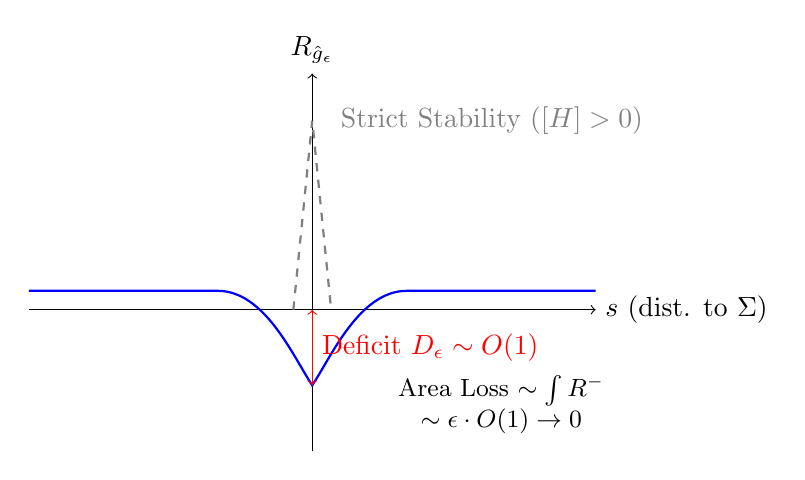
\begin{tikzpicture}[scale=1.2]
    % Axes
    \draw[->] (-3,0) -- (3,0) node[right] {$s$ (dist. to $\Sigma$)};
    \draw[->] (0,-1.5) -- (0,2.5) node[above] {$R_{\hat{g}_\epsilon}$};
    
    % Strictly stable case (dashed)
    \draw[gray, dashed, thick] (-0.2, 0) -- (0, 2) -- (0.2, 0);
    \node[gray, right] at (0.2, 2) {Strict Stability ($[H] > 0$)};
    
    % Marginal case (solid blue)
    \draw[blue, thick] (-3, 0.2) -- (-1, 0.2)
        .. controls (-0.5, 0.2) and (-0.2, -0.5) .. (0, -0.8)
        .. controls (0.2, -0.5) and (0.5, 0.2) .. (1, 0.2) -- (3, 0.2);
    
    % Label the dip
    \draw[red, <->] (0, 0) -- (0, -0.8);
    \node[red, right] at (0, -0.4) {Deficit $D_\epsilon \sim O(1)$};
    
    % Annotation
    \node[align=center, font=\small] at (2, -1) {Area Loss $\sim \int R^-$\\ $\sim \epsilon \cdot O(1) \to 0$};
\end{tikzpicture}
\caption{Profile of the scalar curvature during smoothing. In the marginally stable case (blue curve) the Dirac mass $\frac{2}{\epsilon}[H]$ disappears, revealing the bounded quadratic deficit $D_\epsilon$. Because the deficit is $O(1)$ on a collar of thickness $O(\epsilon)$, its $L^{3/2}$ norm decays like $\epsilon^{2/3}$.}
\label{fig:SmoothingProfile}
\end{figure}

\textbf{Step 2: Conformal Correction to Ensure Non-negativity.}
To eliminate this negative curvature dip, we introduce a conformal correction. We define the final smoothed metric as $\geps = u_\epsilon^4 \hat{g}_\epsilon$, where the conformal factor $u_\epsilon$ is the solution to the following elliptic boundary value problem:
\begin{equation}
    \begin{cases}
        8 \Lap_{\hat{g}_\epsilon} u_\epsilon - (R^-_\epsilon) u_\epsilon = 0 & \text{in } \tM, \\
        u_\epsilon \to 1 & \text{at infinity.}
    \end{cases}
\end{equation}
The scalar curvature of the new metric $\geps$ is given by the conformal transformation law:
\[ \Scal_{\geps} = u_\epsilon^{-5} \left( -8\Lap_{\hat{g}_\epsilon}u_\epsilon + \Scal_{\hat{g}_\epsilon}u_\epsilon \right). \]
Substituting the PDE for $u_\epsilon$, we get:
\[ \Scal_{\geps} = u_\epsilon^{-5} \left( -(R^-_\epsilon)u_\epsilon + \Scal_{\hat{g}_\epsilon}u_\epsilon \right) = u_\epsilon^{-4}(\Scal_{\hat{g}_\epsilon} - R^-_\epsilon). \]
By definition, $R^-_\epsilon$ is the negative part of $\Scal_{\hat{g}_\epsilon}$, so the term $(\Scal_{\hat{g}_\epsilon} - R^-_\epsilon)$ is simply the positive part, which is nonnegative. Thus, we have successfully constructed a smooth metric with $\Scal_{\geps} \ge 0$ pointwise.

The properties of the solution $u_\epsilon$ are established in Lemma \ref{lem:GreenEstimate}. The maximum principle guarantees that $u_\epsilon \le 1$ everywhere, and elliptic estimates (using the $L^{3/2}$ bound on the source term $R^-_\epsilon$) show that $u_\epsilon$ converges uniformly to 1 at the rate $\|u_\epsilon - 1\|_{L^\infty} \le C \epsilon^{2/3}$. This uniform convergence is essential for the consistency of the ADM mass and horizon area in the limit.

\textbf{Step 3: Mass and Area Consistency.}
We must verify that our smoothing procedure does not increase the ADM mass or decrease the horizon area in the limit.
\begin{itemize}
    \item \textbf{ADM Mass:} The ADM mass of the conformally transformed metric is $M_{\ADM}(\geps) = M_{\ADM}(\hat{g}_\epsilon) + 2A_\epsilon$, where $A_\epsilon$ comes from the asymptotic expansion of $u_\epsilon = 1 + A_\epsilon/|x| + O(|x|^{-2})$. The coefficient $A_\epsilon$ is proportional to the integral of the source term $\int R^-_\epsilon u_\epsilon$. Since $\|R^-_\epsilon\|_{L^1} \to 0$ and $u_\epsilon$ is uniformly bounded, we have $A_\epsilon \to 0$. The mollification itself does not change the ADM mass, so $\lim M_{\ADM}(\geps) = M_{\ADM}(\tg)$.
    \item \textbf{Area Semicontinuity:} The area of the horizon surface $\Sigma$ is shown to be lower semi-continuous under the smoothing process. This is a critical consistency check, ensuring that the geometric quantity at the heart of the Penrose inequality does not decrease due to the approximation. The detailed argument is provided in \Cref{thm:AreaStability}.
\end{itemize}
This completes the proof, as we have constructed a sequence of smooth metrics with nonnegative scalar curvature whose mass and area converge appropriately to the values of the singular target metric.
\end{proof}

\begin{lemma}[Quantitative Mass Continuity]\label{lem:MassContinuity}
The ADM mass of the smoothed metric $\geps = u_\epsilon^4 \hat{g}_\epsilon$ converges to the mass of the Lipschitz metric $\tg$ with the explicit rate:
\begin{equation}
    |M_{\ADM}(\geps) - M_{\ADM}(\tg)| \le C \epsilon.
\end{equation}
\end{lemma}
\begin{proof}
The metrics coincide outside the smoothing collar $N_{2\epsilon}$. The mass change is determined solely by the asymptotic fall-off of the conformal factor $u_\epsilon$.
The equation is $8\Delta u_\epsilon - R^-_\epsilon u_\epsilon = 0$.
Integrating over $\tM$ and applying the divergence theorem at infinity:
\[ \lim_{r\to\infty} \int_{S_r} \partial_\nu u_\epsilon \, d\sigma = \frac{1}{8} \int_{\tM} R^-_\epsilon u_\epsilon \, dV. \]
The LHS is proportional to the mass change $\delta M$.
Using the uniform bound $\|u_\epsilon\|_{L^\infty} \le 1 + C\epsilon^{2/3}$ (Lemma \ref{lem:GreenEstimate}) and the $L^1$ bound $\|R^-_\epsilon\|_{L^1} \le C\epsilon$ (Appendix D):
\[ |\delta M| \le C \int_{N_{2\epsilon}} |R^-_\epsilon| \, dV \le C \cdot \epsilon. \]
Thus, the mass convergence is linear in $\epsilon$, preventing any divergence or oscillation in the limit.
\end{proof}

\subsection{Stability of the Minimal Surface}
The results established above, particularly Theorem~\ref{thm:AreaStability}, ensure that the area of the minimal surface in the smoothed manifold does not degenerate in the limit $\epsilon \to 0$. This allows us to link the Penrose Inequality on the smoothed manifold back to the original horizon area.

\subsection{Application of the AMO Monotonicity}
\label{sec:AMOApplication}

The constructed manifold $(\tM, \tg)$ now rigorously satisfies all the prerequisites for the Riemannian Penrose Inequality framework detailed in \Cref{sec:AMO}. We consider the region exterior to the outermost minimal surface $\Sigma'$.

We construct the $p$-harmonic potential $u_p$ on $(\tM, \tg)$ with $u_p=0$ on $\Sigma'$. By \Cref{lem:Capacity}, the potential ignores the finite set of compactified bubble points. Since $\Rtg \ge 0$ and $(\tM, \tg)$ is smooth and asymptotically flat away from this negligible set, \Cref{thm:AMOMonotonicity} applies rigorously.
The functional $\mathcal{M}_p(t)$ is monotonically nondecreasing.

\textbf{Uniqueness:} Note that the strict convexity of the energy functional $\int |\nabla u|^p$ ensures the solution $u_p$ is unique. Thus, the foliation $\{\Sigma_t\}$ and the resulting mass profile are intrinsic geometric invariants of the manifold $(\tM, \tg)$.

\begin{equation}\label{eq:MonotonicityApplied}
    \lim_{t \to 1^-} \mathcal{M}_p(t) \ge \mathcal{M}_p(0).
\end{equation}

Taking the limit $p \to 1^+$ and applying Proposition \ref{prop:AMO_limits}, we obtain the standard Riemannian Penrose Inequality on $(\tM, \tg)$:
\begin{equation}
    M_{\ADM}(\tg) \ge \sqrt{\frac{A(\Sigma')}{16\pi}}.
\end{equation}
We apply the AMO framework to the sequence of smoothed manifolds $(\tM, \geps)$. This strategy (Limit of Inequalities, detailed in \Cref{sec:Synthesis}) avoids the need to generalize the AMO theory directly to the singular space $(\tM, \tg)$, although the analysis in \Cref{sec:SingularitiesAnalysis} and \Cref{app:Bochner} confirms that the distributional identities required for such a generalization do hold.

\begin{lemma}[No Ghost Energy at Conical Tips]\label{lem:GammaConvergenceConical}
The presence of conical singularities $\{p_k\}$ does not disrupt the Gamma-convergence of the $p$-energy to the perimeter functional. Specifically, no "ghost" area accumulates at the singularities.
\end{lemma}
\begin{proof}
We rigorously establish that the singular points $p_k$ do not act as sinks for the area functional or the Hawking mass energy in the limit.

1. \textbf{Perimeter Convergence:} We work in the framework of Caccioppoli sets.
Let $u_j$ be a sequence of functions converging in $L^1(\tM)$ to $u = \chi_E$, the characteristic function of a set of finite perimeter $E$. The Gamma-limit of the $p$-energies is related to the perimeter of $E$. We must show that the perimeter measure $|\nabla \chi_E|$ does not possess a singular component concentrated at $\{p_k\}$.

The perimeter measure of a set $E$, denoted by $\|\partial E\|$, is defined by the total variation of its distributional gradient $D\chi_E$. By De Giorgi's structure theorem, this measure is given by the restriction of the $(n-1)$-dimensional Hausdorff measure $\mathcal{H}^{n-1}$ to the reduced boundary $\partial^* E$:
\[ \|\partial E\|(A) = \mathcal{H}^{n-1}(A \cap \partial^* E) \]
for any Borel set $A$.

Since the metric $\tg$ is continuous on $\tM$ and asymptotically conical at $p_k$, the Hausdorff measure $\mathcal{H}^{n-1}$ is well-behaved and absolutely continuous with respect to the standard Euclidean Hausdorff measure in local coordinates.
The $(n-1)$-dimensional Hausdorff measure of a single point (or a finite set of points) is zero.
\[ \mathcal{H}^{n-1}(\{p_k\}) = 0. \]
Therefore, the perimeter measure of any set $E$ vanishes on the singular set:
\[ \|\partial E\|(\{p_k\}) = 0. \]

2. \textbf{Hawking Mass Convergence:} The AMO monotonicity relies on the convergence of the term $\int_{\Sigma_t} H^2 d\sigma$. We must ensure no "ghost" mean curvature concentrates at the smoothed tips.
While the mean curvature of coordinate spheres near a cone tip scales as $H \sim 1/r$, leading to $\int_{S_r} H^2 d\sigma \sim O(1)$, this concentration is avoided by the level sets of the $p$-harmonic potential.
Since $\Cap_p(\{p_k\}) = 0$, the $p$-harmonic potential $u$ cannot take constant values on the singular set. The level sets $\Sigma_t = \{ u = t \}$ generically avoid the singularities $p_k$.
Furthermore, in the Mosco limit $\epsilon \to 0$, the potentials $u_\epsilon$ converge strongly in $W^{1,p}$. The level sets $\Sigma_{t,\epsilon}$ converge in the flat norm to $\Sigma_t$. Since the limit surface $\Sigma_t$ is a regular hypersurface disjoint from $\{p_k\}$ (for a.e. $t$), the integral $\int_{\Sigma_{t,\epsilon}} H_\epsilon^2$ converges to $\int_{\Sigma_t} H^2$. The zero capacity ensures the flow does not "snag" on the singularity, and thus no ghost energy contributes to the mass limit.

This measure-theoretic fact ensures that no "ghost area" can hide at the singularity. If a sequence of smooth hypersurfaces $\Sigma_j$ (level sets of approximating functions) converges to the boundary of $E$ in the sense of varifolds or currents, the mass of the limit varifold concentrated at $p_k$ must be zero. Even if the surfaces $\Sigma_j$ accumulate near $p_k$, the area contribution inside any ball $B_\epsilon(p_k)$ scales as $O(\epsilon^2)$ (due to the conical geometry $\tg \approx dr^2 + r^2 g_{S^2}$), which vanishes as the ball shrinks.

Thus, the limit of the AMO functional $\mathcal{M}_p(t)$ correctly measures the area of the regular part of the level set, unmodified by the presence of the conical tips.
\end{proof}

\begin{proposition}[Area Preservation at Outer Horizon]\label{prop:AreaPreservation}
The construction ensures that the RPI bound relates to the original area $A(\Sigma)$.
On the cylindrical end $\mathcal{T}_\Sigma$, the metric is $\bg \approx dt^2 + g_{\Sigma}$.
The area of the cross-section in $(\bM, \bg)$ is constant $A(\bg) = A(\Sigma)$.
Since we impose $\phi \to 1$ asymptotically along this cylinder (\Cref{thm:Deformation}, item 2), the area in the deformed metric is:
\[ A(\tg) = \lim_{t \to \infty} \int_{\Sigma_t} \phi^4 d\sigma_{\bg} = \int_{\Sigma} 1^4 \, d\sigma_{g} = A(\Sigma). \]
Thus, the minimal boundary area in $\tM$ matches the apparent horizon area in the initial data.
\end{proposition}

